% Options for packages loaded elsewhere
\PassOptionsToPackage{unicode}{hyperref}
\PassOptionsToPackage{hyphens}{url}
%
\documentclass[
]{book}
\usepackage{lmodern}
\usepackage{amsmath}
\usepackage{ifxetex,ifluatex}
\ifnum 0\ifxetex 1\fi\ifluatex 1\fi=0 % if pdftex
  \usepackage[T1]{fontenc}
  \usepackage[utf8]{inputenc}
  \usepackage{textcomp} % provide euro and other symbols
  \usepackage{amssymb}
\else % if luatex or xetex
  \usepackage{unicode-math}
  \defaultfontfeatures{Scale=MatchLowercase}
  \defaultfontfeatures[\rmfamily]{Ligatures=TeX,Scale=1}
\fi
% Use upquote if available, for straight quotes in verbatim environments
\IfFileExists{upquote.sty}{\usepackage{upquote}}{}
\IfFileExists{microtype.sty}{% use microtype if available
  \usepackage[]{microtype}
  \UseMicrotypeSet[protrusion]{basicmath} % disable protrusion for tt fonts
}{}
\makeatletter
\@ifundefined{KOMAClassName}{% if non-KOMA class
  \IfFileExists{parskip.sty}{%
    \usepackage{parskip}
  }{% else
    \setlength{\parindent}{0pt}
    \setlength{\parskip}{6pt plus 2pt minus 1pt}}
}{% if KOMA class
  \KOMAoptions{parskip=half}}
\makeatother
\usepackage{xcolor}
\IfFileExists{xurl.sty}{\usepackage{xurl}}{} % add URL line breaks if available
\IfFileExists{bookmark.sty}{\usepackage{bookmark}}{\usepackage{hyperref}}
\hypersetup{
  pdftitle={Proyecto LCC-2020/2021},
  pdfauthor={Guillermo Jiménez Jiménez},
  hidelinks,
  pdfcreator={LaTeX via pandoc}}
\urlstyle{same} % disable monospaced font for URLs
\usepackage{color}
\usepackage{fancyvrb}
\newcommand{\VerbBar}{|}
\newcommand{\VERB}{\Verb[commandchars=\\\{\}]}
\DefineVerbatimEnvironment{Highlighting}{Verbatim}{commandchars=\\\{\}}
% Add ',fontsize=\small' for more characters per line
\usepackage{framed}
\definecolor{shadecolor}{RGB}{248,248,248}
\newenvironment{Shaded}{\begin{snugshade}}{\end{snugshade}}
\newcommand{\AlertTok}[1]{\textcolor[rgb]{0.94,0.16,0.16}{#1}}
\newcommand{\AnnotationTok}[1]{\textcolor[rgb]{0.56,0.35,0.01}{\textbf{\textit{#1}}}}
\newcommand{\AttributeTok}[1]{\textcolor[rgb]{0.77,0.63,0.00}{#1}}
\newcommand{\BaseNTok}[1]{\textcolor[rgb]{0.00,0.00,0.81}{#1}}
\newcommand{\BuiltInTok}[1]{#1}
\newcommand{\CharTok}[1]{\textcolor[rgb]{0.31,0.60,0.02}{#1}}
\newcommand{\CommentTok}[1]{\textcolor[rgb]{0.56,0.35,0.01}{\textit{#1}}}
\newcommand{\CommentVarTok}[1]{\textcolor[rgb]{0.56,0.35,0.01}{\textbf{\textit{#1}}}}
\newcommand{\ConstantTok}[1]{\textcolor[rgb]{0.00,0.00,0.00}{#1}}
\newcommand{\ControlFlowTok}[1]{\textcolor[rgb]{0.13,0.29,0.53}{\textbf{#1}}}
\newcommand{\DataTypeTok}[1]{\textcolor[rgb]{0.13,0.29,0.53}{#1}}
\newcommand{\DecValTok}[1]{\textcolor[rgb]{0.00,0.00,0.81}{#1}}
\newcommand{\DocumentationTok}[1]{\textcolor[rgb]{0.56,0.35,0.01}{\textbf{\textit{#1}}}}
\newcommand{\ErrorTok}[1]{\textcolor[rgb]{0.64,0.00,0.00}{\textbf{#1}}}
\newcommand{\ExtensionTok}[1]{#1}
\newcommand{\FloatTok}[1]{\textcolor[rgb]{0.00,0.00,0.81}{#1}}
\newcommand{\FunctionTok}[1]{\textcolor[rgb]{0.00,0.00,0.00}{#1}}
\newcommand{\ImportTok}[1]{#1}
\newcommand{\InformationTok}[1]{\textcolor[rgb]{0.56,0.35,0.01}{\textbf{\textit{#1}}}}
\newcommand{\KeywordTok}[1]{\textcolor[rgb]{0.13,0.29,0.53}{\textbf{#1}}}
\newcommand{\NormalTok}[1]{#1}
\newcommand{\OperatorTok}[1]{\textcolor[rgb]{0.81,0.36,0.00}{\textbf{#1}}}
\newcommand{\OtherTok}[1]{\textcolor[rgb]{0.56,0.35,0.01}{#1}}
\newcommand{\PreprocessorTok}[1]{\textcolor[rgb]{0.56,0.35,0.01}{\textit{#1}}}
\newcommand{\RegionMarkerTok}[1]{#1}
\newcommand{\SpecialCharTok}[1]{\textcolor[rgb]{0.00,0.00,0.00}{#1}}
\newcommand{\SpecialStringTok}[1]{\textcolor[rgb]{0.31,0.60,0.02}{#1}}
\newcommand{\StringTok}[1]{\textcolor[rgb]{0.31,0.60,0.02}{#1}}
\newcommand{\VariableTok}[1]{\textcolor[rgb]{0.00,0.00,0.00}{#1}}
\newcommand{\VerbatimStringTok}[1]{\textcolor[rgb]{0.31,0.60,0.02}{#1}}
\newcommand{\WarningTok}[1]{\textcolor[rgb]{0.56,0.35,0.01}{\textbf{\textit{#1}}}}
\usepackage{longtable,booktabs}
\usepackage{calc} % for calculating minipage widths
% Correct order of tables after \paragraph or \subparagraph
\usepackage{etoolbox}
\makeatletter
\patchcmd\longtable{\par}{\if@noskipsec\mbox{}\fi\par}{}{}
\makeatother
% Allow footnotes in longtable head/foot
\IfFileExists{footnotehyper.sty}{\usepackage{footnotehyper}}{\usepackage{footnote}}
\makesavenoteenv{longtable}
\usepackage{graphicx}
\makeatletter
\def\maxwidth{\ifdim\Gin@nat@width>\linewidth\linewidth\else\Gin@nat@width\fi}
\def\maxheight{\ifdim\Gin@nat@height>\textheight\textheight\else\Gin@nat@height\fi}
\makeatother
% Scale images if necessary, so that they will not overflow the page
% margins by default, and it is still possible to overwrite the defaults
% using explicit options in \includegraphics[width, height, ...]{}
\setkeys{Gin}{width=\maxwidth,height=\maxheight,keepaspectratio}
% Set default figure placement to htbp
\makeatletter
\def\fps@figure{htbp}
\makeatother
\setlength{\emergencystretch}{3em} % prevent overfull lines
\providecommand{\tightlist}{%
  \setlength{\itemsep}{0pt}\setlength{\parskip}{0pt}}
\setcounter{secnumdepth}{5}
\usepackage{booktabs}
\ifluatex
  \usepackage{selnolig}  % disable illegal ligatures
\fi
\usepackage[]{natbib}
\bibliographystyle{apalike}

\title{Proyecto LCC-2020/2021}
\author{Guillermo Jiménez Jiménez}
\date{2021-05-31}

\begin{document}
\maketitle

{
\setcounter{tocdepth}{1}
\tableofcontents
}
\hypertarget{descripciuxf3n-del-proyecto}{%
\chapter{Descripción del proyecto}\label{descripciuxf3n-del-proyecto}}

En este book se encuentran los proyectos acerca de DPLYR, Reglas de asociación, Formal Concept Analysis, Regresión, Text Mining y Social Network Analysis propuestos en la asignatura de Laboratorio de Computación Científica durante el curso 2020-2021.

\hypertarget{aprendizaje-de-r---anuxe1lisis-de-datos}{%
\chapter{Aprendizaje de R - Análisis de Datos}\label{aprendizaje-de-r---anuxe1lisis-de-datos}}

\hypertarget{introducciuxf3n-a-r}{%
\section{Introducción a R}\label{introducciuxf3n-a-r}}

\begin{Shaded}
\begin{Highlighting}[]
\FunctionTok{library}\NormalTok{(tidyverse)}
\end{Highlighting}
\end{Shaded}

\begin{verbatim}
## -- Attaching packages --------------------------------------- tidyverse 1.3.1 --
\end{verbatim}

\begin{verbatim}
## v ggplot2 3.3.3     v purrr   0.3.4
## v tibble  3.1.0     v dplyr   1.0.5
## v tidyr   1.1.3     v stringr 1.4.0
## v readr   1.4.0     v forcats 0.5.1
\end{verbatim}

\begin{verbatim}
## Warning: package 'tidyr' was built under R version 4.0.5
\end{verbatim}

\begin{verbatim}
## Warning: package 'dplyr' was built under R version 4.0.5
\end{verbatim}

\begin{verbatim}
## -- Conflicts ------------------------------------------ tidyverse_conflicts() --
## x dplyr::filter() masks stats::filter()
## x dplyr::lag()    masks stats::lag()
\end{verbatim}

\begin{Shaded}
\begin{Highlighting}[]
\FunctionTok{library}\NormalTok{(readxl)}
\NormalTok{deCV }\OtherTok{\textless{}{-}} \FunctionTok{read\_excel}\NormalTok{(}\StringTok{"deCV.xlsx"}\NormalTok{)}
\end{Highlighting}
\end{Shaded}

\begin{enumerate}
\def\labelenumi{\arabic{enumi}.}
\tightlist
\item
  Eliminar columnas 1, 3, 4,5 y 6 del dataset.
\end{enumerate}

\begin{Shaded}
\begin{Highlighting}[]
\NormalTok{deCV }\OtherTok{\textless{}{-}} \FunctionTok{as.data.frame}\NormalTok{(deCV)}
\NormalTok{deCV }\OtherTok{\textless{}{-}} \FunctionTok{select}\NormalTok{(deCV,}\SpecialCharTok{{-}}\NormalTok{Respuesta,}\SpecialCharTok{{-}}\NormalTok{Institución,}\SpecialCharTok{{-}}\NormalTok{Departamento,}\SpecialCharTok{{-}}\NormalTok{Asignatura,}\SpecialCharTok{{-}}\NormalTok{Grupo)}
\end{Highlighting}
\end{Shaded}

\begin{enumerate}
\def\labelenumi{\arabic{enumi}.}
\setcounter{enumi}{1}
\tightlist
\item
  Cambiar el nombre de la información de las empresas: empresa1,empresa2,empresa3
\end{enumerate}

\begin{Shaded}
\begin{Highlighting}[]
\NormalTok{deCV }\OtherTok{\textless{}{-}} \FunctionTok{rename}\NormalTok{(deCV, }\AttributeTok{empresa1 =}\NormalTok{ Q01\_empresa1, }\AttributeTok{empresa2 =}\NormalTok{ Q02\_empresa2, }\AttributeTok{empresa3 =}\NormalTok{ Q03\_selecion3 )}
\end{Highlighting}
\end{Shaded}

\begin{enumerate}
\def\labelenumi{\arabic{enumi}.}
\setcounter{enumi}{2}
\tightlist
\item
  Cambiar el nombre de la columna con el dni: DNI
\end{enumerate}

\begin{Shaded}
\begin{Highlighting}[]
\NormalTok{deCV }\OtherTok{\textless{}{-}} \FunctionTok{rename}\NormalTok{(deCV, }\AttributeTok{DNI =}\NormalTok{ Documento\_de\_identidad)}
\end{Highlighting}
\end{Shaded}

\begin{enumerate}
\def\labelenumi{\arabic{enumi}.}
\setcounter{enumi}{3}
\tightlist
\item
  Convertir a mayúsculas los datos almacenados en DNI
\end{enumerate}

\begin{Shaded}
\begin{Highlighting}[]
\NormalTok{deCV}\SpecialCharTok{$}\NormalTok{DNI }\OtherTok{\textless{}{-}} \FunctionTok{lapply}\NormalTok{(deCV}\SpecialCharTok{$}\NormalTok{DNI,toupper)}
\end{Highlighting}
\end{Shaded}

\begin{enumerate}
\def\labelenumi{\arabic{enumi}.}
\setcounter{enumi}{4}
\tightlist
\item
  Eliminar la columna con nombre Completado pero sin usar índice la columna, usar su nombre.
\end{enumerate}

\begin{Shaded}
\begin{Highlighting}[]
\NormalTok{deCV }\OtherTok{\textless{}{-}} \FunctionTok{select}\NormalTok{(deCV,}\SpecialCharTok{{-}}\NormalTok{Completado)}
\end{Highlighting}
\end{Shaded}

\begin{enumerate}
\def\labelenumi{\arabic{enumi}.}
\setcounter{enumi}{5}
\tightlist
\item
  Hacer una función que se le pase cada columna y devuelva si contiene algún valor NA.
\end{enumerate}

\begin{Shaded}
\begin{Highlighting}[]
\NormalTok{valorNA }\OtherTok{\textless{}{-}} \ControlFlowTok{function}\NormalTok{(x)\{}
  \FunctionTok{as.logical}\NormalTok{(}\FunctionTok{sum}\NormalTok{(}\FunctionTok{is.na}\NormalTok{(x)))}
\NormalTok{\}}
\FunctionTok{valorNA}\NormalTok{(deCV}\SpecialCharTok{$}\NormalTok{empresa2)}
\end{Highlighting}
\end{Shaded}

\begin{verbatim}
## [1] TRUE
\end{verbatim}

\begin{enumerate}
\def\labelenumi{\arabic{enumi}.}
\setcounter{enumi}{6}
\tightlist
\item
  Ordenar el dataset por nombre del alumno y guardarlo en deCV
\end{enumerate}

\begin{Shaded}
\begin{Highlighting}[]
\NormalTok{deCV }\OtherTok{\textless{}{-}}\NormalTok{ deCV[}\FunctionTok{order}\NormalTok{(deCV}\SpecialCharTok{$}\StringTok{\textasciigrave{}}\AttributeTok{Nombre completo}\StringTok{\textasciigrave{}}\NormalTok{),]}
\end{Highlighting}
\end{Shaded}

\begin{enumerate}
\def\labelenumi{\arabic{enumi}.}
\setcounter{enumi}{7}
\tightlist
\item
  Seleciona de la columna del nombre los 5 primeros alumnos
\end{enumerate}

\begin{Shaded}
\begin{Highlighting}[]
\NormalTok{deCV}\SpecialCharTok{$}\StringTok{\textasciigrave{}}\AttributeTok{Nombre completo}\StringTok{\textasciigrave{}}\NormalTok{[}\DecValTok{1}\SpecialCharTok{:}\DecValTok{5}\NormalTok{]}
\end{Highlighting}
\end{Shaded}

\begin{verbatim}
## [1] "Ana López"         "Ana Rodríguez"     "Antonio Rodríguez"
## [4] "David Aranda"      "Emilio Ruiz"
\end{verbatim}

\begin{enumerate}
\def\labelenumi{\arabic{enumi}.}
\setcounter{enumi}{8}
\tightlist
\item
  Selecciona el dataset correspondiente a los 5 primeros alumnos.
\end{enumerate}

\begin{Shaded}
\begin{Highlighting}[]
\NormalTok{deCV[}\DecValTok{1}\SpecialCharTok{:}\DecValTok{5}\NormalTok{,]}
\end{Highlighting}
\end{Shaded}

\begin{verbatim}
##           Enviado el:    ID   Nombre completo       DNI
## 1 2021-02-28 17:04:37  1234         Ana López 22222222V
## 5 2021-02-28 18:42:17  1234     Ana Rodríguez 12322222V
## 7 2021-02-27 13:02:57 67443 Antonio Rodríguez 66622222V
## 6 2021-02-25 18:06:08  2345      David Aranda 22222999L
## 4 2021-02-26 14:40:50  4322       Emilio Ruiz 11122222V
##                                           empresa1
## 1            24 : 290351\tHISPASEC SISTEMAS, S.L.\t1
## 5                     12 : 290425\tDXC Technology\t2
## 7 40 : 289794\tMALAGA EXCELLENCE & TECHNOLOGY SL.\t4
## 6 42 : 292242\tMALAGA EXCELLENCE & TECHNOLOGY SL.\t3
## 4 40 : 289794\tMALAGA EXCELLENCE & TECHNOLOGY SL.\t4
##                                           empresa2
## 1            22 : 290252\tHISPASEC SISTEMAS, S.L.\t1
## 5                     15 : 290441\tDXC Technology\t2
## 7     54 : 282240\tSoderberg & Partners Spain Sl.\t1
## 6 40 : 289794\tMALAGA EXCELLENCE & TECHNOLOGY SL.\t4
## 4 39 : 289785\tMALAGA EXCELLENCE & TECHNOLOGY SL.\t4
##                                           empresa3
## 1                            33 : 293479\tINGENIA\t1
## 5                              6 : 289123\tCEMOSA\t2
## 7 41 : 289961\tMALAGA EXCELLENCE & TECHNOLOGY SL.\t4
## 6                                             <NA>
## 4                                             <NA>
\end{verbatim}

\begin{enumerate}
\def\labelenumi{\arabic{enumi}.}
\setcounter{enumi}{9}
\tightlist
\item
  Seleciona de la columna del nombre los alumnos que están en las posiciones impares.
\end{enumerate}

\begin{Shaded}
\begin{Highlighting}[]
\NormalTok{deCV}\SpecialCharTok{$}\StringTok{\textasciigrave{}}\AttributeTok{Nombre completo}\StringTok{\textasciigrave{}}\NormalTok{[}\FunctionTok{c}\NormalTok{(}\ConstantTok{TRUE}\NormalTok{,}\ConstantTok{FALSE}\NormalTok{)]}
\end{Highlighting}
\end{Shaded}

\begin{verbatim}
## [1] "Ana López"         "Antonio Rodríguez" "Emilio Ruiz"      
## [4] "Felix Nogales"     "Mercedes Laviña"
\end{verbatim}

\begin{enumerate}
\def\labelenumi{\arabic{enumi}.}
\setcounter{enumi}{10}
\tightlist
\item
  Selecciona el dataset correspondiente a los alumnos que están en las posiciones impares.
\end{enumerate}

\begin{Shaded}
\begin{Highlighting}[]
\NormalTok{deCV[}\FunctionTok{c}\NormalTok{(}\ConstantTok{TRUE}\NormalTok{,}\ConstantTok{FALSE}\NormalTok{),]}
\end{Highlighting}
\end{Shaded}

\begin{verbatim}
##            Enviado el:    ID   Nombre completo       DNI
## 1  2021-02-28 17:04:37  1234         Ana López 22222222V
## 7  2021-02-27 13:02:57 67443 Antonio Rodríguez 66622222V
## 4  2021-02-26 14:40:50  4322       Emilio Ruiz 11122222V
## 10 2021-02-25 15:45:13  3444     Felix Nogales 97652222T
## 9  2021-02-28 12:05:30 32222   Mercedes Laviña 82766666A
##                                            empresa1
## 1             24 : 290351\tHISPASEC SISTEMAS, S.L.\t1
## 7  40 : 289794\tMALAGA EXCELLENCE & TECHNOLOGY SL.\t4
## 4  40 : 289794\tMALAGA EXCELLENCE & TECHNOLOGY SL.\t4
## 10                     44 : 291702\tNEWRALERS S.L.\t3
## 9          51 : 291565\tRAVENPACK INTERNATIONAL SL\t1
##                                            empresa2
## 1             22 : 290252\tHISPASEC SISTEMAS, S.L.\t1
## 7      54 : 282240\tSoderberg & Partners Spain Sl.\t1
## 4  39 : 289785\tMALAGA EXCELLENCE & TECHNOLOGY SL.\t4
## 10         50 : 291560\tRAVENPACK INTERNATIONAL SL\t1
## 9                      44 : 291702\tNEWRALERS S.L.\t3
##                                            empresa3
## 1                             33 : 293479\tINGENIA\t1
## 7  41 : 289961\tMALAGA EXCELLENCE & TECHNOLOGY SL.\t4
## 4                                              <NA>
## 10         51 : 291565\tRAVENPACK INTERNATIONAL SL\t1
## 9                                              <NA>
\end{verbatim}

\begin{enumerate}
\def\labelenumi{\arabic{enumi}.}
\setcounter{enumi}{11}
\tightlist
\item
  Añadir una columna num\_empresas que contenga cuantas empresas ha selecionado cada alumno.
\end{enumerate}

\begin{Shaded}
\begin{Highlighting}[]
\NormalTok{numeroempresasfila }\OtherTok{\textless{}{-}} \ControlFlowTok{function}\NormalTok{(x)\{}
   \FunctionTok{sum}\NormalTok{(}\SpecialCharTok{!}\FunctionTok{is.na}\NormalTok{(deCV[x, }\FunctionTok{c}\NormalTok{(}\StringTok{"empresa1"}\NormalTok{, }\StringTok{"empresa2"}\NormalTok{, }\StringTok{"empresa3"}\NormalTok{)]))}
  
\NormalTok{\}}
\NormalTok{filas }\OtherTok{\textless{}{-}} \DecValTok{1}\SpecialCharTok{:}\FunctionTok{dim}\NormalTok{(deCV)[}\DecValTok{1}\NormalTok{]}


\CommentTok{\#deCV \textless{}{-} mutate(deCV,"num\_empresas"=numeroempresasfila(filas))   }

\NormalTok{columna }\OtherTok{\textless{}{-}} \FunctionTok{sapply}\NormalTok{(filas,numeroempresasfila)}
\NormalTok{deCV}\SpecialCharTok{$}\NormalTok{num\_empresas }\OtherTok{\textless{}{-}}\NormalTok{ columna}
\end{Highlighting}
\end{Shaded}

\begin{enumerate}
\def\labelenumi{\arabic{enumi}.}
\setcounter{enumi}{12}
\tightlist
\item
  Haz una función que devuelva los índices de la columna empresa1, empresa2, empresa3 que contienen
  valores NA.
\end{enumerate}

\begin{Shaded}
\begin{Highlighting}[]
\NormalTok{indiceNA }\OtherTok{\textless{}{-}} \ControlFlowTok{function}\NormalTok{(x)\{}
  \FunctionTok{which}\NormalTok{(}\FunctionTok{is.na}\NormalTok{(deCV[x, }\FunctionTok{c}\NormalTok{(}\StringTok{"empresa1"}\NormalTok{, }\StringTok{"empresa2"}\NormalTok{, }\StringTok{"empresa3"}\NormalTok{)]))}
\NormalTok{\}}
\NormalTok{filas }\OtherTok{\textless{}{-}} \DecValTok{1}\SpecialCharTok{:}\FunctionTok{dim}\NormalTok{(deCV)[}\DecValTok{1}\NormalTok{]}
\FunctionTok{sapply}\NormalTok{(filas,indiceNA)}
\end{Highlighting}
\end{Shaded}

\begin{verbatim}
## [[1]]
## integer(0)
## 
## [[2]]
## integer(0)
## 
## [[3]]
## integer(0)
## 
## [[4]]
## [1] 3
## 
## [[5]]
## [1] 3
## 
## [[6]]
## [1] 2 3
## 
## [[7]]
## integer(0)
## 
## [[8]]
## integer(0)
## 
## [[9]]
## [1] 3
## 
## [[10]]
## integer(0)
\end{verbatim}

\begin{enumerate}
\def\labelenumi{\arabic{enumi}.}
\setcounter{enumi}{13}
\tightlist
\item
  Calcular la media de las empresas seleccionadas por todos los alumnos a partir de la información
  recolectada en num\_empresas
\end{enumerate}

\begin{Shaded}
\begin{Highlighting}[]
\NormalTok{media }\OtherTok{\textless{}{-}} \FunctionTok{sapply}\NormalTok{(}\FunctionTok{list}\NormalTok{(deCV}\SpecialCharTok{$}\NormalTok{num\_empresas),mean)}
\NormalTok{media}
\end{Highlighting}
\end{Shaded}

\begin{verbatim}
## [1] 2.5
\end{verbatim}

\begin{enumerate}
\def\labelenumi{\arabic{enumi}.}
\setcounter{enumi}{14}
\tightlist
\item
  Calcular la media de aquellos valores de num\_empresas que estén por encima de la media e indicar los
  nombres de los alumnos que superan esa media.
\end{enumerate}

\begin{Shaded}
\begin{Highlighting}[]
\NormalTok{mayorquemedia }\OtherTok{\textless{}{-}} \FunctionTok{filter}\NormalTok{(deCV,num\_empresas}\SpecialCharTok{\textgreater{}}\NormalTok{media)[}\StringTok{"Nombre completo"}\NormalTok{]}
\NormalTok{mayorquemedia}
\end{Highlighting}
\end{Shaded}

\begin{verbatim}
##      Nombre completo
## 1          Ana López
## 2      Ana Rodríguez
## 3  Antonio Rodríguez
## 4      Felix Nogales
## 5      Lucía Mercado
## 6 Miguel Ángel Luque
\end{verbatim}

\begin{enumerate}
\def\labelenumi{\arabic{enumi}.}
\setcounter{enumi}{15}
\tightlist
\item
  Cambiar valores NA por 0 en todo el dataset
\end{enumerate}

\begin{Shaded}
\begin{Highlighting}[]
\NormalTok{cambia\_na }\OtherTok{\textless{}{-}} \ControlFlowTok{function}\NormalTok{(x)\{}
  \FunctionTok{ifelse}\NormalTok{(}\FunctionTok{is.na}\NormalTok{(x),}\DecValTok{0}\NormalTok{,x)}
\NormalTok{\}}
\NormalTok{deCV }\OtherTok{\textless{}{-}} \FunctionTok{sapply}\NormalTok{(deCV,cambia\_na)}
\end{Highlighting}
\end{Shaded}

\hypertarget{dplyr}{%
\section{DPLYR}\label{dplyr}}

\begin{Shaded}
\begin{Highlighting}[]
\FunctionTok{library}\NormalTok{(tidyverse)}
\FunctionTok{data}\NormalTok{(}\StringTok{"starwars"}\NormalTok{)}
\FunctionTok{View}\NormalTok{(starwars)}
\end{Highlighting}
\end{Shaded}

1.Obtener los 10 humanos más viejos, masculinos, con planeta natal Tatooine.

\begin{Shaded}
\begin{Highlighting}[]
\NormalTok{starwars }\SpecialCharTok{\%\textgreater{}\%}
 \FunctionTok{filter}\NormalTok{(species}\SpecialCharTok{==}\StringTok{"Human"} \SpecialCharTok{\&}\NormalTok{ gender }\SpecialCharTok{==} \StringTok{"masculine"} \SpecialCharTok{\&}\NormalTok{ homeworld }\SpecialCharTok{==} \StringTok{"Tatooine"}\NormalTok{) }\SpecialCharTok{\%\textgreater{}\%}
 \FunctionTok{arrange}\NormalTok{(birth\_year) }\SpecialCharTok{\%\textgreater{}\%}
 \FunctionTok{slice}\NormalTok{(}\DecValTok{1}\SpecialCharTok{:}\DecValTok{10}\NormalTok{)}
\end{Highlighting}
\end{Shaded}

\begin{verbatim}
## # A tibble: 6 x 14
##   name     height  mass hair_color  skin_color eye_color birth_year sex   gender
##   <chr>     <int> <dbl> <chr>       <chr>      <chr>          <dbl> <chr> <chr> 
## 1 Luke Sk~    172    77 blond       fair       blue            19   male  mascu~
## 2 Biggs D~    183    84 black       light      brown           24   male  mascu~
## 3 Darth V~    202   136 none        white      yellow          41.9 male  mascu~
## 4 Anakin ~    188    84 blond       fair       blue            41.9 male  mascu~
## 5 Owen La~    178   120 brown, grey light      blue            52   male  mascu~
## 6 Cliegg ~    183    NA brown       fair       blue            82   male  mascu~
## # ... with 5 more variables: homeworld <chr>, species <chr>, films <list>,
## #   vehicles <list>, starships <list>
\end{verbatim}

2.Encontrar a aquellos personajes de ojos azules y rubios/as de especie humana, procedentes de Tatooine, ordenados por edad de menor a mayor. Calcular su altura media.

\begin{Shaded}
\begin{Highlighting}[]
\NormalTok{st1 }\OtherTok{\textless{}{-}}\NormalTok{ starwars }\SpecialCharTok{\%\textgreater{}\%}
  \FunctionTok{filter}\NormalTok{(species}\SpecialCharTok{==}\StringTok{"Human"} \SpecialCharTok{\&}\NormalTok{ eye\_color}\SpecialCharTok{==}\StringTok{"blue"} \SpecialCharTok{\&}\NormalTok{ hair\_color}\SpecialCharTok{==}\StringTok{"blond"} \SpecialCharTok{|}\NormalTok{ hair\_color}\SpecialCharTok{==}\StringTok{"blonde"}\NormalTok{ , homeworld}\SpecialCharTok{==}\StringTok{"Tatooine"}\NormalTok{)}\SpecialCharTok{\%\textgreater{}\%}
  \FunctionTok{arrange}\NormalTok{(}\FunctionTok{desc}\NormalTok{(birth\_year))}
\NormalTok{st1}
\end{Highlighting}
\end{Shaded}

\begin{verbatim}
## # A tibble: 2 x 14
##   name      height  mass hair_color skin_color eye_color birth_year sex   gender
##   <chr>      <int> <dbl> <chr>      <chr>      <chr>          <dbl> <chr> <chr> 
## 1 Anakin S~    188    84 blond      fair       blue            41.9 male  mascu~
## 2 Luke Sky~    172    77 blond      fair       blue            19   male  mascu~
## # ... with 5 more variables: homeworld <chr>, species <chr>, films <list>,
## #   vehicles <list>, starships <list>
\end{verbatim}

\begin{Shaded}
\begin{Highlighting}[]
\NormalTok{st1}\SpecialCharTok{\%\textgreater{}\%}\FunctionTok{summarise}\NormalTok{(}\FunctionTok{mean}\NormalTok{(height))}
\end{Highlighting}
\end{Shaded}

\begin{verbatim}
## # A tibble: 1 x 1
##   `mean(height)`
##            <dbl>
## 1            180
\end{verbatim}

3.Encontrar aquellos personajes de especie Human o Naboo y calcular una variable con los valores pesado o ligero (si su massa es mayor que 79 es pesado). Mostrar las variables name, height mass y heavyorlight y ordenar por mass de mayor a menor.

\begin{Shaded}
\begin{Highlighting}[]
\NormalTok{HumanNaboo }\OtherTok{\textless{}{-}}\NormalTok{ starwars }\SpecialCharTok{\%\textgreater{}\%}
  \FunctionTok{filter}\NormalTok{(species}\SpecialCharTok{==}\StringTok{"Human"} \SpecialCharTok{|}\NormalTok{ species }\SpecialCharTok{==}\StringTok{"Naboo"}\NormalTok{)}
\NormalTok{HumanNaboo}
\end{Highlighting}
\end{Shaded}

\begin{verbatim}
## # A tibble: 35 x 14
##    name    height  mass hair_color  skin_color eye_color birth_year sex   gender
##    <chr>    <int> <dbl> <chr>       <chr>      <chr>          <dbl> <chr> <chr> 
##  1 Luke S~    172    77 blond       fair       blue            19   male  mascu~
##  2 Darth ~    202   136 none        white      yellow          41.9 male  mascu~
##  3 Leia O~    150    49 brown       light      brown           19   fema~ femin~
##  4 Owen L~    178   120 brown, grey light      blue            52   male  mascu~
##  5 Beru W~    165    75 brown       light      blue            47   fema~ femin~
##  6 Biggs ~    183    84 black       light      brown           24   male  mascu~
##  7 Obi-Wa~    182    77 auburn, wh~ fair       blue-gray       57   male  mascu~
##  8 Anakin~    188    84 blond       fair       blue            41.9 male  mascu~
##  9 Wilhuf~    180    NA auburn, gr~ fair       blue            64   male  mascu~
## 10 Han So~    180    80 brown       fair       brown           29   male  mascu~
## # ... with 25 more rows, and 5 more variables: homeworld <chr>, species <chr>,
## #   films <list>, vehicles <list>, starships <list>
\end{verbatim}

\begin{Shaded}
\begin{Highlighting}[]
\NormalTok{pesadoligero }\OtherTok{\textless{}{-}} \ControlFlowTok{function}\NormalTok{(x)\{}
  
  \FunctionTok{ifelse}\NormalTok{(x}\SpecialCharTok{\textgreater{}}\DecValTok{79}\NormalTok{,}\StringTok{"pesado"}\NormalTok{,}\StringTok{"ligero"}\NormalTok{)}
  
\NormalTok{\}}
\NormalTok{HumanNaboo }\OtherTok{\textless{}{-}} \FunctionTok{mutate}\NormalTok{(HumanNaboo,}\AttributeTok{heavyorlight =} \FunctionTok{pesadoligero}\NormalTok{(mass))}

\FunctionTok{select}\NormalTok{(HumanNaboo, name, height, mass, heavyorlight) }\SpecialCharTok{\%\textgreater{}\%} \FunctionTok{arrange}\NormalTok{(}\FunctionTok{desc}\NormalTok{(mass))}
\end{Highlighting}
\end{Shaded}

\begin{verbatim}
## # A tibble: 35 x 4
##    name              height  mass heavyorlight
##    <chr>              <int> <dbl> <chr>       
##  1 Darth Vader          202   136 pesado      
##  2 Owen Lars            178   120 pesado      
##  3 Jek Tono Porkins     180   110 pesado      
##  4 Qui-Gon Jinn         193    89 pesado      
##  5 Gregar Typho         185    85 pesado      
##  6 Biggs Darklighter    183    84 pesado      
##  7 Anakin Skywalker     188    84 pesado      
##  8 Mace Windu           188    84 pesado      
##  9 Han Solo             180    80 pesado      
## 10 Dooku                193    80 pesado      
## # ... with 25 more rows
\end{verbatim}

4.Calcular el indice de masa corporal de todos los personajes (eliminando los que tienen masa o altura NA). A continuación mostrar el nombre, altura, masa y IMC de cada personaje, con orden de IMC descendente.

\begin{Shaded}
\begin{Highlighting}[]
\CommentTok{\#masa/(talla\^{}2)}
\NormalTok{imc }\OtherTok{\textless{}{-}} \ControlFlowTok{function}\NormalTok{(x,y)\{}
\NormalTok{  res }\OtherTok{\textless{}{-}}\NormalTok{ (x}\SpecialCharTok{/}\NormalTok{((y)}\SpecialCharTok{/}\DecValTok{100}\NormalTok{)}\SpecialCharTok{\^{}}\DecValTok{2}\NormalTok{)}
  \FunctionTok{return}\NormalTok{(res)}
\NormalTok{\}}
\NormalTok{personajesSinMasaAlturaNA }\OtherTok{\textless{}{-}}\NormalTok{ starwars }\SpecialCharTok{\%\textgreater{}\%} \FunctionTok{filter}\NormalTok{(}\SpecialCharTok{!}\FunctionTok{is.na}\NormalTok{(mass) }\SpecialCharTok{\&} \SpecialCharTok{!}\FunctionTok{is.na}\NormalTok{(height))}
\NormalTok{personajesSinMasaAlturaNA }\OtherTok{\textless{}{-}} \FunctionTok{mutate}\NormalTok{(personajesSinMasaAlturaNA,}\AttributeTok{IMC =} \FunctionTok{imc}\NormalTok{(mass,height)) }\SpecialCharTok{\%\textgreater{}\%} \FunctionTok{arrange}\NormalTok{(}\FunctionTok{desc}\NormalTok{(IMC)) }\SpecialCharTok{\%\textgreater{}\%} \FunctionTok{select}\NormalTok{(name,height, mass, IMC)}
\NormalTok{personajesSinMasaAlturaNA}
\end{Highlighting}
\end{Shaded}

\begin{verbatim}
## # A tibble: 59 x 4
##    name                  height  mass   IMC
##    <chr>                  <int> <dbl> <dbl>
##  1 Jabba Desilijic Tiure    175  1358 443. 
##  2 Dud Bolt                  94    45  50.9
##  3 Yoda                      66    17  39.0
##  4 Owen Lars                178   120  37.9
##  5 IG-88                    200   140  35  
##  6 R2-D2                     96    32  34.7
##  7 Grievous                 216   159  34.1
##  8 R5-D4                     97    32  34.0
##  9 Jek Tono Porkins         180   110  34.0
## 10 Darth Vader              202   136  33.3
## # ... with 49 more rows
\end{verbatim}

5.Obtener los personajes cuya única nave fuese un X-wing y ordenarlos de forma descendente según su masa

\begin{Shaded}
\begin{Highlighting}[]
\NormalTok{starwars }\SpecialCharTok{\%\textgreater{}\%} \FunctionTok{filter}\NormalTok{(starships}\SpecialCharTok{==}\StringTok{"X{-}wing"}\NormalTok{) }\SpecialCharTok{\%\textgreater{}\%} \FunctionTok{arrange}\NormalTok{(}\FunctionTok{desc}\NormalTok{(mass))}
\end{Highlighting}
\end{Shaded}

\begin{verbatim}
## # A tibble: 3 x 14
##   name      height  mass hair_color skin_color eye_color birth_year sex   gender
##   <chr>      <int> <dbl> <chr>      <chr>      <chr>          <dbl> <chr> <chr> 
## 1 Jek Tono~    180   110 brown      fair       blue              NA male  mascu~
## 2 Biggs Da~    183    84 black      light      brown             24 male  mascu~
## 3 Wedge An~    170    77 brown      fair       hazel             21 male  mascu~
## # ... with 5 more variables: homeworld <chr>, species <chr>, films <list>,
## #   vehicles <list>, starships <list>
\end{verbatim}

6.Obtener los personajes de masa superior a la media de las masas, obviando valores nulos, y ordenarlos de forma decreciente.

\begin{Shaded}
\begin{Highlighting}[]
\NormalTok{sinNulos }\OtherTok{\textless{}{-}}\NormalTok{ starwars }\SpecialCharTok{\%\textgreater{}\%} \FunctionTok{filter}\NormalTok{(}\SpecialCharTok{!}\FunctionTok{is.na}\NormalTok{(mass))}
\NormalTok{sinNulos}
\end{Highlighting}
\end{Shaded}

\begin{verbatim}
## # A tibble: 59 x 14
##    name    height  mass hair_color  skin_color eye_color birth_year sex   gender
##    <chr>    <int> <dbl> <chr>       <chr>      <chr>          <dbl> <chr> <chr> 
##  1 Luke S~    172    77 blond       fair       blue            19   male  mascu~
##  2 C-3PO      167    75 <NA>        gold       yellow         112   none  mascu~
##  3 R2-D2       96    32 <NA>        white, bl~ red             33   none  mascu~
##  4 Darth ~    202   136 none        white      yellow          41.9 male  mascu~
##  5 Leia O~    150    49 brown       light      brown           19   fema~ femin~
##  6 Owen L~    178   120 brown, grey light      blue            52   male  mascu~
##  7 Beru W~    165    75 brown       light      blue            47   fema~ femin~
##  8 R5-D4       97    32 <NA>        white, red red             NA   none  mascu~
##  9 Biggs ~    183    84 black       light      brown           24   male  mascu~
## 10 Obi-Wa~    182    77 auburn, wh~ fair       blue-gray       57   male  mascu~
## # ... with 49 more rows, and 5 more variables: homeworld <chr>, species <chr>,
## #   films <list>, vehicles <list>, starships <list>
\end{verbatim}

\begin{Shaded}
\begin{Highlighting}[]
\NormalTok{media }\OtherTok{\textless{}{-}} \FunctionTok{lapply}\NormalTok{(sinNulos[}\StringTok{"mass"}\NormalTok{],mean)}
\CommentTok{\#media}
\NormalTok{sinNulos }\SpecialCharTok{\%\textgreater{}\%} \FunctionTok{filter}\NormalTok{(mass}\SpecialCharTok{\textgreater{}}\NormalTok{media) }\SpecialCharTok{\%\textgreater{}\%} \FunctionTok{arrange}\NormalTok{(}\FunctionTok{desc}\NormalTok{(mass))}
\end{Highlighting}
\end{Shaded}

\begin{verbatim}
## # A tibble: 10 x 14
##    name    height  mass hair_color  skin_color eye_color birth_year sex   gender
##    <chr>    <int> <dbl> <chr>       <chr>      <chr>          <dbl> <chr> <chr> 
##  1 Jabba ~    175  1358 <NA>        green-tan~ orange         600   herm~ mascu~
##  2 Grievo~    216   159 none        brown, wh~ green, y~       NA   male  mascu~
##  3 IG-88      200   140 none        metal      red             15   none  mascu~
##  4 Darth ~    202   136 none        white      yellow          41.9 male  mascu~
##  5 Tarfful    234   136 brown       brown      blue            NA   male  mascu~
##  6 Owen L~    178   120 brown, grey light      blue            52   male  mascu~
##  7 Bossk      190   113 none        green      red             53   male  mascu~
##  8 Chewba~    228   112 brown       unknown    blue           200   male  mascu~
##  9 Jek To~    180   110 brown       fair       blue            NA   male  mascu~
## 10 Dexter~    198   102 none        brown      yellow          NA   male  mascu~
## # ... with 5 more variables: homeworld <chr>, species <chr>, films <list>,
## #   vehicles <list>, starships <list>
\end{verbatim}

7.Obtener las alturas medias de los personajes con el campo ``gender'' igual a ``female'', ``male'' y ``hermaphrodite'', ignorando NA.

--El campo que contiene los valores ``female'',``male'' y ``hermaphroditic'' es `sex', no `gender'

\begin{Shaded}
\begin{Highlighting}[]
\NormalTok{alturasGeneroSinNA }\OtherTok{\textless{}{-}}\NormalTok{ starwars }\SpecialCharTok{\%\textgreater{}\%} \FunctionTok{filter}\NormalTok{(}\SpecialCharTok{!}\FunctionTok{is.na}\NormalTok{(height) }\SpecialCharTok{\&} \SpecialCharTok{!}\FunctionTok{is.na}\NormalTok{(gender) }\SpecialCharTok{\&}\NormalTok{ (sex}\SpecialCharTok{==}\StringTok{"female"} \SpecialCharTok{|}\NormalTok{ sex }\SpecialCharTok{==}\StringTok{"male"} \SpecialCharTok{|}\NormalTok{ sex}\SpecialCharTok{==}\StringTok{"hermaphroditic"}\NormalTok{))}
\NormalTok{alturasGeneroSinNA}
\end{Highlighting}
\end{Shaded}

\begin{verbatim}
## # A tibble: 73 x 14
##    name    height  mass hair_color  skin_color eye_color birth_year sex   gender
##    <chr>    <int> <dbl> <chr>       <chr>      <chr>          <dbl> <chr> <chr> 
##  1 Luke S~    172    77 blond       fair       blue            19   male  mascu~
##  2 Darth ~    202   136 none        white      yellow          41.9 male  mascu~
##  3 Leia O~    150    49 brown       light      brown           19   fema~ femin~
##  4 Owen L~    178   120 brown, grey light      blue            52   male  mascu~
##  5 Beru W~    165    75 brown       light      blue            47   fema~ femin~
##  6 Biggs ~    183    84 black       light      brown           24   male  mascu~
##  7 Obi-Wa~    182    77 auburn, wh~ fair       blue-gray       57   male  mascu~
##  8 Anakin~    188    84 blond       fair       blue            41.9 male  mascu~
##  9 Wilhuf~    180    NA auburn, gr~ fair       blue            64   male  mascu~
## 10 Chewba~    228   112 brown       unknown    blue           200   male  mascu~
## # ... with 63 more rows, and 5 more variables: homeworld <chr>, species <chr>,
## #   films <list>, vehicles <list>, starships <list>
\end{verbatim}

\begin{Shaded}
\begin{Highlighting}[]
\NormalTok{females }\OtherTok{\textless{}{-}}\NormalTok{ alturasGeneroSinNA }\SpecialCharTok{\%\textgreater{}\%} \FunctionTok{filter}\NormalTok{(sex}\SpecialCharTok{==}\StringTok{"female"}\NormalTok{)}
\NormalTok{males }\OtherTok{\textless{}{-}}\NormalTok{ alturasGeneroSinNA }\SpecialCharTok{\%\textgreater{}\%} \FunctionTok{filter}\NormalTok{(sex}\SpecialCharTok{==}\StringTok{"male"}\NormalTok{)}
\NormalTok{hermaphroditic }\OtherTok{\textless{}{-}}\NormalTok{ alturasGeneroSinNA }\SpecialCharTok{\%\textgreater{}\%} \FunctionTok{filter}\NormalTok{(sex}\SpecialCharTok{==}\StringTok{"hermaphroditic"}\NormalTok{)}
\NormalTok{mediaFemales }\OtherTok{\textless{}{-}} \FunctionTok{lapply}\NormalTok{(females[}\StringTok{"height"}\NormalTok{],mean)}
\NormalTok{mediaFemales}
\end{Highlighting}
\end{Shaded}

\begin{verbatim}
## $height
## [1] 169.2667
\end{verbatim}

\begin{Shaded}
\begin{Highlighting}[]
\NormalTok{mediaMales }\OtherTok{\textless{}{-}} \FunctionTok{lapply}\NormalTok{(males[}\StringTok{"height"}\NormalTok{],mean)}
\NormalTok{mediaMales}
\end{Highlighting}
\end{Shaded}

\begin{verbatim}
## $height
## [1] 179.1053
\end{verbatim}

\begin{Shaded}
\begin{Highlighting}[]
\NormalTok{mediaHermaphoditics }\OtherTok{\textless{}{-}} \FunctionTok{lapply}\NormalTok{(hermaphroditic[}\StringTok{"height"}\NormalTok{],mean)}
\NormalTok{mediaHermaphoditics}
\end{Highlighting}
\end{Shaded}

\begin{verbatim}
## $height
## [1] 175
\end{verbatim}

8.Filtrar por las especies que sean ``Droid'', ordenados por altura descendiente y masa. Reemplazar las masas y alturas con valor NA por 1 y mostrar solo la media de todas esas masas y la mediana de esas alturas.

\begin{Shaded}
\begin{Highlighting}[]
\NormalTok{droides }\OtherTok{\textless{}{-}}\NormalTok{ starwars }\SpecialCharTok{\%\textgreater{}\%} \FunctionTok{filter}\NormalTok{(species}\SpecialCharTok{==}\StringTok{"Droid"}\NormalTok{) }\SpecialCharTok{\%\textgreater{}\%} \FunctionTok{arrange}\NormalTok{(}\FunctionTok{desc}\NormalTok{(height),}\FunctionTok{desc}\NormalTok{(mass)) }\SpecialCharTok{\%\textgreater{}\%} \FunctionTok{select}\NormalTok{(name,mass,height)}
\CommentTok{\#droides}
\NormalTok{cambiarNA }\OtherTok{\textless{}{-}} \ControlFlowTok{function}\NormalTok{(x)\{}
  \FunctionTok{ifelse}\NormalTok{(}\FunctionTok{is.na}\NormalTok{(x),}\DecValTok{1}\NormalTok{,x)}
\NormalTok{\}}
\NormalTok{droides }\OtherTok{\textless{}{-}} \FunctionTok{lapply}\NormalTok{(droides,cambiarNA)}
\CommentTok{\#droides}
\NormalTok{media }\OtherTok{\textless{}{-}} \FunctionTok{sapply}\NormalTok{(droides[}\StringTok{"mass"}\NormalTok{],mean)}
\NormalTok{media}
\end{Highlighting}
\end{Shaded}

\begin{verbatim}
##     mass 
## 46.83333
\end{verbatim}

\begin{Shaded}
\begin{Highlighting}[]
\NormalTok{mediana }\OtherTok{\textless{}{-}} \FunctionTok{sapply}\NormalTok{(droides[}\StringTok{"height"}\NormalTok{],median)}
\NormalTok{mediana}
\end{Highlighting}
\end{Shaded}

\begin{verbatim}
## height 
##   96.5
\end{verbatim}

9.Sacar aquellas filas con las cadenas ``Jedi'' ó ``Clones'' en la columna films. Agrupar por homeworld y sacar la media de la columnas height y mass (por separado). Reemplazar los valores NA en la columna mass por 0.

\begin{Shaded}
\begin{Highlighting}[]
\NormalTok{cambiarNACero }\OtherTok{\textless{}{-}} \ControlFlowTok{function}\NormalTok{(x)\{}
  \FunctionTok{ifelse}\NormalTok{(}\FunctionTok{is.na}\NormalTok{(x),}\DecValTok{0}\NormalTok{,x)}
\NormalTok{\}}
\NormalTok{filmJediClones}\OtherTok{\textless{}{-}}\NormalTok{ starwars }\SpecialCharTok{\%\textgreater{}\%} \FunctionTok{filter}\NormalTok{(}\FunctionTok{grepl}\NormalTok{(}\StringTok{"Jedi"}\NormalTok{,films) }\SpecialCharTok{|} \FunctionTok{grepl}\NormalTok{(}\StringTok{"Clones"}\NormalTok{,films)) }

\NormalTok{filmJediClones}\OtherTok{\textless{}{-}}\NormalTok{ filmJediClones }\SpecialCharTok{\%\textgreater{}\%} \FunctionTok{group\_by}\NormalTok{(homeworld) }\SpecialCharTok{\%\textgreater{}\%} \FunctionTok{summarise}\NormalTok{(}\AttributeTok{Numero\_Personajes =} \FunctionTok{n}\NormalTok{(), }\AttributeTok{Media\_Altura =} \FunctionTok{mean}\NormalTok{(height), }\AttributeTok{Media\_Mass =} \FunctionTok{mean}\NormalTok{(mass))}


\NormalTok{filmJediClones[}\StringTok{"Media\_Mass"}\NormalTok{] }\OtherTok{\textless{}{-}}  \FunctionTok{sapply}\NormalTok{(filmJediClones[}\StringTok{"Media\_Mass"}\NormalTok{],cambiarNACero)}
\NormalTok{filmJediClones}
\end{Highlighting}
\end{Shaded}

\begin{verbatim}
## # A tibble: 33 x 4
##    homeworld      Numero_Personajes Media_Altura Media_Mass
##    <chr>                      <int>        <dbl>      <dbl>
##  1 Alderaan                       2         170.        0  
##  2 Cato Neimoidia                 1         191        90  
##  3 Cerea                          1         198        82  
##  4 Champala                       1         196         0  
##  5 Chandrila                      1         150         0  
##  6 Concord Dawn                   1         183        79  
##  7 Corellia                       2         175        78.5
##  8 Coruscant                      1         167         0  
##  9 Dorin                          1         188        80  
## 10 Endor                          1          88        20  
## # ... with 23 more rows
\end{verbatim}

10.Filtrar los datos de aquellos personajes que hayan aparecido solo en la película ``Return of the Jedi''y que tengan un mundo natal, ordenados por peso. Para ello transforma los valores NA en 0.

\begin{Shaded}
\begin{Highlighting}[]
\NormalTok{personajesReturnJedi }\OtherTok{\textless{}{-}}\NormalTok{ starwars }\SpecialCharTok{\%\textgreater{}\%} \FunctionTok{filter}\NormalTok{(films}\SpecialCharTok{==}\StringTok{"Return of the Jedi"} \SpecialCharTok{\&} \SpecialCharTok{!}\FunctionTok{is.na}\NormalTok{(homeworld))}
\NormalTok{personajesReturnJedi[}\StringTok{"mass"}\NormalTok{] }\OtherTok{\textless{}{-}} \FunctionTok{sapply}\NormalTok{(personajesReturnJedi[}\StringTok{"mass"}\NormalTok{], cambiarNACero)}
\NormalTok{personajesReturnJedi}\OtherTok{\textless{}{-}}\NormalTok{ personajesReturnJedi }\SpecialCharTok{\%\textgreater{}\%} \FunctionTok{arrange}\NormalTok{(mass)}
\NormalTok{personajesReturnJedi}
\end{Highlighting}
\end{Shaded}

\begin{verbatim}
## # A tibble: 4 x 14
##   name      height  mass hair_color skin_color eye_color birth_year sex   gender
##   <chr>      <int> <dbl> <chr>      <chr>      <chr>          <dbl> <chr> <chr> 
## 1 Mon Moth~    150     0 auburn     fair       blue              48 fema~ femin~
## 2 Bib Fort~    180     0 none       pale       pink              NA male  mascu~
## 3 Wicket S~     88    20 brown      brown      brown              8 male  mascu~
## 4 Nien Nunb    160    68 none       grey       black             NA male  mascu~
## # ... with 5 more variables: homeworld <chr>, species <chr>, films <list>,
## #   vehicles <list>, starships <list>
\end{verbatim}

11.Seleccionar los humanos que midan más de 170 cm y que hayan salido en Attack of the Clones, agrupandolos por homeworld obviando los NA y hallar la media de sus pesos sustituyendo los NA por la mediana y mostrarlos en orden descendiente.

\begin{Shaded}
\begin{Highlighting}[]
\NormalTok{humanosAttackClones}\OtherTok{\textless{}{-}}\NormalTok{ starwars }\SpecialCharTok{\%\textgreater{}\%} \FunctionTok{filter}\NormalTok{(species}\SpecialCharTok{==}\StringTok{"Human"} \SpecialCharTok{\&}\NormalTok{ height}\SpecialCharTok{\textgreater{}}\DecValTok{170} \SpecialCharTok{\&} \FunctionTok{grepl}\NormalTok{(}\StringTok{"Attack of the Clones"}\NormalTok{,films))}
 
\NormalTok{humanosAttackClones}\OtherTok{\textless{}{-}}\NormalTok{ humanosAttackClones }\SpecialCharTok{\%\textgreater{}\%} \FunctionTok{group\_by}\NormalTok{(homeworld) }\SpecialCharTok{\%\textgreater{}\%} \FunctionTok{summarise}\NormalTok{(}\AttributeTok{Numero\_Humanos =} \FunctionTok{n}\NormalTok{(), }\AttributeTok{Media\_Pesos =} \FunctionTok{mean}\NormalTok{(mass))}

\NormalTok{cambiarNAMediana }\OtherTok{\textless{}{-}} \ControlFlowTok{function}\NormalTok{(x)\{}
  \FunctionTok{ifelse}\NormalTok{(}\FunctionTok{is.na}\NormalTok{(x),}\FunctionTok{median}\NormalTok{(x),x)}
\NormalTok{\}}

\NormalTok{humanosAttackClones[}\StringTok{"Media\_Pesos"}\NormalTok{] }\OtherTok{\textless{}{-}} \FunctionTok{sapply}\NormalTok{(humanosAttackClones[}\StringTok{"Media\_Pesos"}\NormalTok{],cambiarNAMediana)}
\NormalTok{humanosAttackClones }\OtherTok{\textless{}{-}}\NormalTok{ humanosAttackClones }\SpecialCharTok{\%\textgreater{}\%} \FunctionTok{arrange}\NormalTok{(}\FunctionTok{desc}\NormalTok{(Media\_Pesos))}
\NormalTok{humanosAttackClones}
\end{Highlighting}
\end{Shaded}

\begin{verbatim}
## # A tibble: 8 x 3
##   homeworld    Numero_Humanos Media_Pesos
##   <chr>                 <int>       <dbl>
## 1 Naboo                     1        85  
## 2 Haruun Kal                1        84  
## 3 Serenno                   1        80  
## 4 Concord Dawn              1        79  
## 5 Kamino                    1        78.2
## 6 Stewjon                   1        77  
## 7 Alderaan                  1        NA  
## 8 Tatooine                  3        NA
\end{verbatim}

12.Encontrar para cada homeworld cuantas especies diferentes lo habitan y ordenalos de mayor a menor variedad. Controlar que no se tiene en cuenta NA como especie

\begin{Shaded}
\begin{Highlighting}[]
\NormalTok{especiesSinNA }\OtherTok{\textless{}{-}}\NormalTok{ starwars }\SpecialCharTok{\%\textgreater{}\%} \FunctionTok{filter}\NormalTok{(}\SpecialCharTok{!}\FunctionTok{is.na}\NormalTok{(species) }\SpecialCharTok{\&} \SpecialCharTok{!}\FunctionTok{is.na}\NormalTok{(homeworld) )}

\NormalTok{especiesSinNA }\OtherTok{\textless{}{-}}\NormalTok{ especiesSinNA }\SpecialCharTok{\%\textgreater{}\%} \FunctionTok{group\_by}\NormalTok{(homeworld) }\SpecialCharTok{\%\textgreater{}\%} \FunctionTok{summarise}\NormalTok{(}\AttributeTok{Numero\_Especies =} \FunctionTok{n}\NormalTok{()) }\SpecialCharTok{\%\textgreater{}\%} \FunctionTok{arrange}\NormalTok{(}\FunctionTok{desc}\NormalTok{(Numero\_Especies))}
\NormalTok{especiesSinNA}
\end{Highlighting}
\end{Shaded}

\begin{verbatim}
## # A tibble: 47 x 2
##    homeworld   Numero_Especies
##    <chr>                 <int>
##  1 Tatooine                 10
##  2 Naboo                     9
##  3 Alderaan                  3
##  4 Coruscant                 3
##  5 Kamino                    3
##  6 Corellia                  2
##  7 Kashyyyk                  2
##  8 Mirial                    2
##  9 Ryloth                    2
## 10 Aleen Minor               1
## # ... with 37 more rows
\end{verbatim}

13.Filtrar a los personajes mayores de 25, y luego ordenarlos por el número de películas en el que aparecen (dato que no viene directamente y tenemos que obtenerlo).

\begin{Shaded}
\begin{Highlighting}[]
\NormalTok{personajes25 }\OtherTok{\textless{}{-}}\NormalTok{ starwars }\SpecialCharTok{\%\textgreater{}\%} \FunctionTok{filter}\NormalTok{(birth\_year}\SpecialCharTok{\textgreater{}}\DecValTok{25}\NormalTok{)}
\NormalTok{personajes25}
\end{Highlighting}
\end{Shaded}

\begin{verbatim}
## # A tibble: 36 x 14
##    name    height  mass hair_color  skin_color eye_color birth_year sex   gender
##    <chr>    <int> <dbl> <chr>       <chr>      <chr>          <dbl> <chr> <chr> 
##  1 C-3PO      167    75 <NA>        gold       yellow         112   none  mascu~
##  2 R2-D2       96    32 <NA>        white, bl~ red             33   none  mascu~
##  3 Darth ~    202   136 none        white      yellow          41.9 male  mascu~
##  4 Owen L~    178   120 brown, grey light      blue            52   male  mascu~
##  5 Beru W~    165    75 brown       light      blue            47   fema~ femin~
##  6 Obi-Wa~    182    77 auburn, wh~ fair       blue-gray       57   male  mascu~
##  7 Anakin~    188    84 blond       fair       blue            41.9 male  mascu~
##  8 Wilhuf~    180    NA auburn, gr~ fair       blue            64   male  mascu~
##  9 Chewba~    228   112 brown       unknown    blue           200   male  mascu~
## 10 Han So~    180    80 brown       fair       brown           29   male  mascu~
## # ... with 26 more rows, and 5 more variables: homeworld <chr>, species <chr>,
## #   films <list>, vehicles <list>, starships <list>
\end{verbatim}

\begin{Shaded}
\begin{Highlighting}[]
\NormalTok{contarPeliculas }\OtherTok{\textless{}{-}} \ControlFlowTok{function}\NormalTok{(x)\{}
\NormalTok{  l }\OtherTok{\textless{}{-}} \FunctionTok{length}\NormalTok{(personajes25}\SpecialCharTok{$}\NormalTok{films[[x]])}
  \FunctionTok{return}\NormalTok{(l)}
\NormalTok{\}}
\NormalTok{filas }\OtherTok{\textless{}{-}} \DecValTok{1}\SpecialCharTok{:}\FunctionTok{dim}\NormalTok{(personajes25)[}\DecValTok{1}\NormalTok{]}

\NormalTok{listaPelis }\OtherTok{\textless{}{-}} \FunctionTok{sapply}\NormalTok{(filas,contarPeliculas)}

\NormalTok{personajes25 }\OtherTok{\textless{}{-}}  \FunctionTok{mutate}\NormalTok{(personajes25, }\AttributeTok{Numero\_Peliculas =}\NormalTok{ listaPelis)}
\NormalTok{personajes25 }\OtherTok{\textless{}{-}}\NormalTok{ personajes25 }\SpecialCharTok{\%\textgreater{}\%} \FunctionTok{arrange}\NormalTok{(Numero\_Peliculas)}

\NormalTok{personajes25}
\end{Highlighting}
\end{Shaded}

\begin{verbatim}
## # A tibble: 36 x 15
##    name    height  mass hair_color skin_color eye_color birth_year sex    gender
##    <chr>    <int> <dbl> <chr>      <chr>      <chr>          <dbl> <chr>  <chr> 
##  1 Greedo     173    74 <NA>       green      black             44 male   mascu~
##  2 Bossk      190   113 none       green      red               53 male   mascu~
##  3 Lobot      175    79 none       light      blue              37 male   mascu~
##  4 Mon Mo~    150    NA auburn     fair       blue              48 female femin~
##  5 Qui-Go~    193    89 brown      fair       blue              92 male   mascu~
##  6 Finis ~    170    NA blond      fair       blue              91 male   mascu~
##  7 Quarsh~    183    NA black      dark       brown             62 <NA>   <NA>  
##  8 Darth ~    175    80 none       red        yellow            54 male   mascu~
##  9 Cliegg~    183    NA brown      fair       blue              82 male   mascu~
## 10 Barris~    166    50 black      yellow     blue              40 female femin~
## # ... with 26 more rows, and 6 more variables: homeworld <chr>, species <chr>,
## #   films <list>, vehicles <list>, starships <list>, Numero_Peliculas <int>
\end{verbatim}

14.Encontrar cuantas especies diferentes habitan cada homeworld y ordenarlos de mayor a menor variedad, controlando que NA no es una especie.

\begin{Shaded}
\begin{Highlighting}[]
\NormalTok{especiesSinNA }\OtherTok{\textless{}{-}}\NormalTok{ starwars }\SpecialCharTok{\%\textgreater{}\%} \FunctionTok{filter}\NormalTok{(}\SpecialCharTok{!}\FunctionTok{is.na}\NormalTok{(species) }\SpecialCharTok{\&} \SpecialCharTok{!}\FunctionTok{is.na}\NormalTok{(homeworld) )}
\NormalTok{especiesSinNA }\SpecialCharTok{\%\textgreater{}\%} \FunctionTok{group\_by}\NormalTok{(homeworld) }\SpecialCharTok{\%\textgreater{}\%} \FunctionTok{summarise}\NormalTok{(}\AttributeTok{n =} \FunctionTok{n}\NormalTok{()) }\SpecialCharTok{\%\textgreater{}\%} \FunctionTok{arrange}\NormalTok{(}\FunctionTok{desc}\NormalTok{(n))}
\end{Highlighting}
\end{Shaded}

\begin{verbatim}
## # A tibble: 47 x 2
##    homeworld       n
##    <chr>       <int>
##  1 Tatooine       10
##  2 Naboo           9
##  3 Alderaan        3
##  4 Coruscant       3
##  5 Kamino          3
##  6 Corellia        2
##  7 Kashyyyk        2
##  8 Mirial          2
##  9 Ryloth          2
## 10 Aleen Minor     1
## # ... with 37 more rows
\end{verbatim}

15.De todos los personajes de Star Wars filtrar por los que tengan mass mayor o igual a 70, agruparlos por species y gender y calcular la media de height de estos (eliminando los valores NA previamente). Mostrar el resultado ordenado de mayor a menor altura

\begin{Shaded}
\begin{Highlighting}[]
\CommentTok{\#Filtrado mass\textgreater{}=70 quitando valores NA}
\NormalTok{massMayor70 }\OtherTok{\textless{}{-}}\NormalTok{ starwars }\SpecialCharTok{\%\textgreater{}\%} \FunctionTok{filter}\NormalTok{(mass}\SpecialCharTok{\textgreater{}=}\DecValTok{70} \SpecialCharTok{\&} \SpecialCharTok{!}\FunctionTok{is.na}\NormalTok{(height) }\SpecialCharTok{\&} \SpecialCharTok{!}\FunctionTok{is.na}\NormalTok{(species) }\SpecialCharTok{\&} \SpecialCharTok{!}\FunctionTok{is.na}\NormalTok{(gender))}
\NormalTok{massMayor70}
\end{Highlighting}
\end{Shaded}

\begin{verbatim}
## # A tibble: 39 x 14
##    name    height  mass hair_color  skin_color eye_color birth_year sex   gender
##    <chr>    <int> <dbl> <chr>       <chr>      <chr>          <dbl> <chr> <chr> 
##  1 Luke S~    172    77 blond       fair       blue            19   male  mascu~
##  2 C-3PO      167    75 <NA>        gold       yellow         112   none  mascu~
##  3 Darth ~    202   136 none        white      yellow          41.9 male  mascu~
##  4 Owen L~    178   120 brown, grey light      blue            52   male  mascu~
##  5 Beru W~    165    75 brown       light      blue            47   fema~ femin~
##  6 Biggs ~    183    84 black       light      brown           24   male  mascu~
##  7 Obi-Wa~    182    77 auburn, wh~ fair       blue-gray       57   male  mascu~
##  8 Anakin~    188    84 blond       fair       blue            41.9 male  mascu~
##  9 Chewba~    228   112 brown       unknown    blue           200   male  mascu~
## 10 Han So~    180    80 brown       fair       brown           29   male  mascu~
## # ... with 29 more rows, and 5 more variables: homeworld <chr>, species <chr>,
## #   films <list>, vehicles <list>, starships <list>
\end{verbatim}

\begin{Shaded}
\begin{Highlighting}[]
\CommentTok{\#Agrupados por especies}
\NormalTok{massMayor70Species }\OtherTok{\textless{}{-}}\NormalTok{ starwars }\SpecialCharTok{\%\textgreater{}\%} \FunctionTok{filter}\NormalTok{(mass}\SpecialCharTok{\textgreater{}=}\DecValTok{70} \SpecialCharTok{\&} \SpecialCharTok{!}\FunctionTok{is.na}\NormalTok{(height) }\SpecialCharTok{\&} \SpecialCharTok{!}\FunctionTok{is.na}\NormalTok{(species) }\SpecialCharTok{\&} \SpecialCharTok{!}\FunctionTok{is.na}\NormalTok{(gender)) }\SpecialCharTok{\%\textgreater{}\%} \FunctionTok{group\_by}\NormalTok{(species) }\SpecialCharTok{\%\textgreater{}\%} \FunctionTok{summarise}\NormalTok{(}\AttributeTok{n =} \FunctionTok{n}\NormalTok{()) }
\NormalTok{massMayor70Species}
\end{Highlighting}
\end{Shaded}

\begin{verbatim}
## # A tibble: 18 x 2
##    species          n
##    <chr>        <int>
##  1 Besalisk         1
##  2 Cerean           1
##  3 Droid            2
##  4 Geonosian        1
##  5 Gungan           1
##  6 Human           20
##  7 Hutt             1
##  8 Kaleesh          1
##  9 Kaminoan         1
## 10 Kel Dor          1
## 11 Mon Calamari     1
## 12 Nautolan         1
## 13 Neimodian        1
## 14 Pau'an           1
## 15 Rodian           1
## 16 Trandoshan       1
## 17 Wookiee          2
## 18 Zabrak           1
\end{verbatim}

\begin{Shaded}
\begin{Highlighting}[]
\CommentTok{\#Agrupados por gender}
\NormalTok{massMayor70Gender }\OtherTok{\textless{}{-}}\NormalTok{ starwars }\SpecialCharTok{\%\textgreater{}\%} \FunctionTok{filter}\NormalTok{(mass}\SpecialCharTok{\textgreater{}=}\DecValTok{70} \SpecialCharTok{\&} \SpecialCharTok{!}\FunctionTok{is.na}\NormalTok{(height) }\SpecialCharTok{\&} \SpecialCharTok{!}\FunctionTok{is.na}\NormalTok{(species) }\SpecialCharTok{\&} \SpecialCharTok{!}\FunctionTok{is.na}\NormalTok{(gender)) }\SpecialCharTok{\%\textgreater{}\%} \FunctionTok{group\_by}\NormalTok{(gender) }\SpecialCharTok{\%\textgreater{}\%} \FunctionTok{summarise}\NormalTok{(}\AttributeTok{n =} \FunctionTok{n}\NormalTok{()) }
\NormalTok{massMayor70Gender}
\end{Highlighting}
\end{Shaded}

\begin{verbatim}
## # A tibble: 2 x 2
##   gender        n
##   <chr>     <int>
## 1 feminine      1
## 2 masculine    38
\end{verbatim}

\begin{Shaded}
\begin{Highlighting}[]
\CommentTok{\#Altura media}
\NormalTok{mediaAltura }\OtherTok{\textless{}{-}} \FunctionTok{sapply}\NormalTok{(massMayor70[}\StringTok{"height"}\NormalTok{],mean)}
\NormalTok{mediaAltura}
\end{Highlighting}
\end{Shaded}

\begin{verbatim}
##   height 
## 189.3846
\end{verbatim}

16.Filtrar por aquellos personajes que tienen los ojos azules y un homeworld y birth\_year asignados (diferentes de NA)

\begin{Shaded}
\begin{Highlighting}[]
\NormalTok{personajesFiltrados }\OtherTok{\textless{}{-}}\NormalTok{ starwars }\SpecialCharTok{\%\textgreater{}\%} \FunctionTok{filter}\NormalTok{(eye\_color}\SpecialCharTok{==}\StringTok{"blue"} \SpecialCharTok{\&} \SpecialCharTok{!}\FunctionTok{is.na}\NormalTok{(homeworld) }\SpecialCharTok{\&} \SpecialCharTok{!}\FunctionTok{is.na}\NormalTok{(birth\_year))}
\NormalTok{personajesFiltrados}
\end{Highlighting}
\end{Shaded}

\begin{verbatim}
## # A tibble: 12 x 14
##    name     height  mass hair_color skin_color eye_color birth_year sex   gender
##    <chr>     <int> <dbl> <chr>      <chr>      <chr>          <dbl> <chr> <chr> 
##  1 Luke Sk~    172  77   blond      fair       blue            19   male  mascu~
##  2 Owen La~    178 120   brown, gr~ light      blue            52   male  mascu~
##  3 Beru Wh~    165  75   brown      light      blue            47   fema~ femin~
##  4 Anakin ~    188  84   blond      fair       blue            41.9 male  mascu~
##  5 Wilhuff~    180  NA   auburn, g~ fair       blue            64   male  mascu~
##  6 Chewbac~    228 112   brown      unknown    blue           200   male  mascu~
##  7 Lobot       175  79   none       light      blue            37   male  mascu~
##  8 Mon Mot~    150  NA   auburn     fair       blue            48   fema~ femin~
##  9 Finis V~    170  NA   blond      fair       blue            91   male  mascu~
## 10 Cliegg ~    183  NA   brown      fair       blue            82   male  mascu~
## 11 Luminar~    170  56.2 black      yellow     blue            58   fema~ femin~
## 12 Barriss~    166  50   black      yellow     blue            40   fema~ femin~
## # ... with 5 more variables: homeworld <chr>, species <chr>, films <list>,
## #   vehicles <list>, starships <list>
\end{verbatim}

-Añadir una columna ficticia en la que se indica la edad que tendrían si no hubiesen muerto y actualmente -estemos en 2019, es decir, restar a 2019 su año de nacimiento

\begin{Shaded}
\begin{Highlighting}[]
\NormalTok{personajesFiltrados }\OtherTok{\textless{}{-}}  \FunctionTok{mutate}\NormalTok{(personajesFiltrados, }\AttributeTok{edad\_Actual =}\NormalTok{ (}\DecValTok{2019}\SpecialCharTok{{-}}\NormalTok{personajesFiltrados}\SpecialCharTok{$}\NormalTok{birth\_year))}
\end{Highlighting}
\end{Shaded}

-Agrupar según el país dónde viven

\begin{Shaded}
\begin{Highlighting}[]
\NormalTok{personajesFiltrados }\SpecialCharTok{\%\textgreater{}\%} \FunctionTok{group\_by}\NormalTok{(homeworld) }\SpecialCharTok{\%\textgreater{}\%} \FunctionTok{summarise}\NormalTok{(}\AttributeTok{n =} \FunctionTok{n}\NormalTok{())}
\end{Highlighting}
\end{Shaded}

\begin{verbatim}
## # A tibble: 7 x 2
##   homeworld     n
##   <chr>     <int>
## 1 Bespin        1
## 2 Chandrila     1
## 3 Coruscant     1
## 4 Eriadu        1
## 5 Kashyyyk      1
## 6 Mirial        2
## 7 Tatooine      5
\end{verbatim}

-Obtener como resultado la media de los valores height, mass y la columna edad previamente calculada

\begin{Shaded}
\begin{Highlighting}[]
\NormalTok{mediaHeight }\OtherTok{\textless{}{-}} \FunctionTok{sapply}\NormalTok{(personajesFiltrados[}\StringTok{"height"}\NormalTok{],mean)}
\NormalTok{mediaHeight}
\end{Highlighting}
\end{Shaded}

\begin{verbatim}
##   height 
## 177.0833
\end{verbatim}

\begin{Shaded}
\begin{Highlighting}[]
\NormalTok{mediaMass }\OtherTok{\textless{}{-}} \FunctionTok{sapply}\NormalTok{(}\FunctionTok{na.omit}\NormalTok{(personajesFiltrados[}\StringTok{"mass"}\NormalTok{]),mean)}
\NormalTok{mediaMass}
\end{Highlighting}
\end{Shaded}

\begin{verbatim}
##  mass 
## 81.65
\end{verbatim}

\begin{Shaded}
\begin{Highlighting}[]
\NormalTok{mediaEdadActual }\OtherTok{\textless{}{-}} \FunctionTok{sapply}\NormalTok{(personajesFiltrados[}\StringTok{"edad\_Actual"}\NormalTok{],mean)}
\NormalTok{mediaEdadActual}
\end{Highlighting}
\end{Shaded}

\begin{verbatim}
## edad_Actual 
##    1954.008
\end{verbatim}

-Ordenar por la columna mass de forma descendentemente

\begin{Shaded}
\begin{Highlighting}[]
\NormalTok{personajesFiltrados }\SpecialCharTok{\%\textgreater{}\%} \FunctionTok{arrange}\NormalTok{(}\FunctionTok{desc}\NormalTok{(mass))}
\end{Highlighting}
\end{Shaded}

\begin{verbatim}
## # A tibble: 12 x 15
##    name     height  mass hair_color skin_color eye_color birth_year sex   gender
##    <chr>     <int> <dbl> <chr>      <chr>      <chr>          <dbl> <chr> <chr> 
##  1 Owen La~    178 120   brown, gr~ light      blue            52   male  mascu~
##  2 Chewbac~    228 112   brown      unknown    blue           200   male  mascu~
##  3 Anakin ~    188  84   blond      fair       blue            41.9 male  mascu~
##  4 Lobot       175  79   none       light      blue            37   male  mascu~
##  5 Luke Sk~    172  77   blond      fair       blue            19   male  mascu~
##  6 Beru Wh~    165  75   brown      light      blue            47   fema~ femin~
##  7 Luminar~    170  56.2 black      yellow     blue            58   fema~ femin~
##  8 Barriss~    166  50   black      yellow     blue            40   fema~ femin~
##  9 Wilhuff~    180  NA   auburn, g~ fair       blue            64   male  mascu~
## 10 Mon Mot~    150  NA   auburn     fair       blue            48   fema~ femin~
## 11 Finis V~    170  NA   blond      fair       blue            91   male  mascu~
## 12 Cliegg ~    183  NA   brown      fair       blue            82   male  mascu~
## # ... with 6 more variables: homeworld <chr>, species <chr>, films <list>,
## #   vehicles <list>, starships <list>, edad_Actual <dbl>
\end{verbatim}

17.Sustituir los valores NA del peso y la altura por la media de todos los pesos y alturas respectivamente.

\begin{Shaded}
\begin{Highlighting}[]
\NormalTok{starwars2}\OtherTok{=}\NormalTok{starwars}
\NormalTok{mediaPesos }\OtherTok{\textless{}{-}} \FunctionTok{sapply}\NormalTok{(}\FunctionTok{na.omit}\NormalTok{(starwars2[}\StringTok{"mass"}\NormalTok{]),mean)}
\NormalTok{mediaAlturas }\OtherTok{\textless{}{-}} \FunctionTok{sapply}\NormalTok{(}\FunctionTok{na.omit}\NormalTok{(starwars2[}\StringTok{"height"}\NormalTok{]),mean)}

\NormalTok{cambiarNAPeso }\OtherTok{\textless{}{-}} \ControlFlowTok{function}\NormalTok{(x)\{}
  \FunctionTok{ifelse}\NormalTok{(}\FunctionTok{is.na}\NormalTok{(x),mediaPesos,x)}
\NormalTok{\}}

\NormalTok{cambiarNAAltura }\OtherTok{\textless{}{-}} \ControlFlowTok{function}\NormalTok{(x)\{}
  \FunctionTok{ifelse}\NormalTok{(}\FunctionTok{is.na}\NormalTok{(x),mediaAlturas,x)}
\NormalTok{\}}

\NormalTok{starwars2[}\StringTok{"mass"}\NormalTok{] }\OtherTok{\textless{}{-}} \FunctionTok{sapply}\NormalTok{(starwars[}\StringTok{"mass"}\NormalTok{],cambiarNAPeso)}
\NormalTok{starwars2[}\StringTok{"height"}\NormalTok{] }\OtherTok{\textless{}{-}} \FunctionTok{sapply}\NormalTok{(starwars[}\StringTok{"height"}\NormalTok{],cambiarNAAltura)}
\end{Highlighting}
\end{Shaded}

Filtrar los humanos cuyo peso sea mayor o igual a 70, agrupados por homeworld,

\begin{Shaded}
\begin{Highlighting}[]
\NormalTok{humanosFiltrados }\OtherTok{\textless{}{-}}\NormalTok{ starwars2 }\SpecialCharTok{\%\textgreater{}\%} \FunctionTok{filter}\NormalTok{(species}\SpecialCharTok{==}\StringTok{"Human"} \SpecialCharTok{\&}\NormalTok{ mass}\SpecialCharTok{\textgreater{}=}\DecValTok{70} \SpecialCharTok{\&} \SpecialCharTok{!}\FunctionTok{is.na}\NormalTok{(homeworld)) }\SpecialCharTok{\%\textgreater{}\%} \FunctionTok{group\_by}\NormalTok{(homeworld) }\SpecialCharTok{\%\textgreater{}\%} \FunctionTok{arrange}\NormalTok{(homeworld)}
\NormalTok{humanosFiltrados}
\end{Highlighting}
\end{Shaded}

\begin{verbatim}
## # A tibble: 28 x 14
## # Groups:   homeworld [15]
##    name     height  mass hair_color skin_color eye_color birth_year sex   gender
##    <chr>     <dbl> <dbl> <chr>      <chr>      <chr>          <dbl> <chr> <chr> 
##  1 Bail Pr~    191  97.3 black      tan        brown             67 male  mascu~
##  2 Raymus ~    188  79   brown      light      brown             NA male  mascu~
##  3 Lobot       175  79   none       light      blue              37 male  mascu~
##  4 Jek Ton~    180 110   brown      fair       blue              NA male  mascu~
##  5 Mon Mot~    150  97.3 auburn     fair       blue              48 fema~ femin~
##  6 Jango F~    183  79   black      tan        brown             66 male  mascu~
##  7 Han Solo    180  80   brown      fair       brown             29 male  mascu~
##  8 Wedge A~    170  77   brown      fair       hazel             21 male  mascu~
##  9 Finis V~    170  97.3 blond      fair       blue              91 male  mascu~
## 10 Jocasta~    167  97.3 white      fair       blue              NA fema~ femin~
## # ... with 18 more rows, and 5 more variables: homeworld <chr>, species <chr>,
## #   films <list>, vehicles <list>, starships <list>
\end{verbatim}

calcular la mediana de la altura y el número de humanos de cada homeworld.

\begin{Shaded}
\begin{Highlighting}[]
\NormalTok{humanosFiltradosMediana }\OtherTok{\textless{}{-}}\NormalTok{  starwars2 }\SpecialCharTok{\%\textgreater{}\%} \FunctionTok{filter}\NormalTok{(species}\SpecialCharTok{==}\StringTok{"Human"} \SpecialCharTok{\&}\NormalTok{ mass}\SpecialCharTok{\textgreater{}=}\DecValTok{70} \SpecialCharTok{\&} \SpecialCharTok{!}\FunctionTok{is.na}\NormalTok{(homeworld)) }\SpecialCharTok{\%\textgreater{}\%} \FunctionTok{group\_by}\NormalTok{(homeworld) }\SpecialCharTok{\%\textgreater{}\%} \FunctionTok{summarise}\NormalTok{(}\AttributeTok{medianaAltura =} \FunctionTok{median}\NormalTok{(height),número}\AttributeTok{\_Humanos =} \FunctionTok{n}\NormalTok{())}
\NormalTok{humanosFiltradosMediana}
\end{Highlighting}
\end{Shaded}

\begin{verbatim}
## # A tibble: 15 x 3
##    homeworld    medianaAltura número_Humanos
##    <chr>                <dbl>          <int>
##  1 Alderaan              190.              2
##  2 Bespin                175               1
##  3 Bestine IV            180               1
##  4 Chandrila             150               1
##  5 Concord Dawn          183               1
##  6 Corellia              175               2
##  7 Coruscant             168.              2
##  8 Eriadu                180               1
##  9 Haruun Kal            188               1
## 10 Kamino                183               1
## 11 Naboo                 168.              4
## 12 Serenno               193               1
## 13 Socorro               177               1
## 14 Stewjon               182               1
## 15 Tatooine              180.              8
\end{verbatim}

Ordenar por número de humanos que hay en cada homeworld.

\begin{Shaded}
\begin{Highlighting}[]
\NormalTok{humanosFiltradosMediana }\SpecialCharTok{\%\textgreater{}\%} \FunctionTok{arrange}\NormalTok{(número\_Humanos)}
\end{Highlighting}
\end{Shaded}

\begin{verbatim}
## # A tibble: 15 x 3
##    homeworld    medianaAltura número_Humanos
##    <chr>                <dbl>          <int>
##  1 Bespin                175               1
##  2 Bestine IV            180               1
##  3 Chandrila             150               1
##  4 Concord Dawn          183               1
##  5 Eriadu                180               1
##  6 Haruun Kal            188               1
##  7 Kamino                183               1
##  8 Serenno               193               1
##  9 Socorro               177               1
## 10 Stewjon               182               1
## 11 Alderaan              190.              2
## 12 Corellia              175               2
## 13 Coruscant             168.              2
## 14 Naboo                 168.              4
## 15 Tatooine              180.              8
\end{verbatim}

18.Obtener todos los humanos, quitando los que su altura es NA

\begin{Shaded}
\begin{Highlighting}[]
\NormalTok{humanos }\OtherTok{\textless{}{-}}\NormalTok{ starwars }\SpecialCharTok{\%\textgreater{}\%} \FunctionTok{filter}\NormalTok{(}\SpecialCharTok{!}\FunctionTok{is.na}\NormalTok{(height) }\SpecialCharTok{\&}\NormalTok{ species}\SpecialCharTok{==}\StringTok{"Human"} \SpecialCharTok{\&} \SpecialCharTok{!}\FunctionTok{is.na}\NormalTok{(homeworld))}
\NormalTok{humanos}
\end{Highlighting}
\end{Shaded}

\begin{verbatim}
## # A tibble: 30 x 14
##    name    height  mass hair_color  skin_color eye_color birth_year sex   gender
##    <chr>    <int> <dbl> <chr>       <chr>      <chr>          <dbl> <chr> <chr> 
##  1 Luke S~    172    77 blond       fair       blue            19   male  mascu~
##  2 Darth ~    202   136 none        white      yellow          41.9 male  mascu~
##  3 Leia O~    150    49 brown       light      brown           19   fema~ femin~
##  4 Owen L~    178   120 brown, grey light      blue            52   male  mascu~
##  5 Beru W~    165    75 brown       light      blue            47   fema~ femin~
##  6 Biggs ~    183    84 black       light      brown           24   male  mascu~
##  7 Obi-Wa~    182    77 auburn, wh~ fair       blue-gray       57   male  mascu~
##  8 Anakin~    188    84 blond       fair       blue            41.9 male  mascu~
##  9 Wilhuf~    180    NA auburn, gr~ fair       blue            64   male  mascu~
## 10 Han So~    180    80 brown       fair       brown           29   male  mascu~
## # ... with 20 more rows, and 5 more variables: homeworld <chr>, species <chr>,
## #   films <list>, vehicles <list>, starships <list>
\end{verbatim}

Añadir una columna con la diferencia entre su altura y la altura media de los humanos

\begin{Shaded}
\begin{Highlighting}[]
\NormalTok{alturaMediaHumanos }\OtherTok{\textless{}{-}} \FunctionTok{sapply}\NormalTok{(humanos[}\StringTok{"height"}\NormalTok{],mean)}
\NormalTok{alturaMediaHumanos}
\end{Highlighting}
\end{Shaded}

\begin{verbatim}
## height 
##  176.1
\end{verbatim}

\begin{Shaded}
\begin{Highlighting}[]
\NormalTok{humanos }\OtherTok{\textless{}{-}}\NormalTok{ humanos }\SpecialCharTok{\%\textgreater{}\%} \FunctionTok{mutate}\NormalTok{(}\AttributeTok{Diferencia\_Altura\_Media =} \FunctionTok{abs}\NormalTok{(humanos}\SpecialCharTok{$}\NormalTok{height}\SpecialCharTok{{-}}\NormalTok{alturaMediaHumanos))}
\NormalTok{humanos}
\end{Highlighting}
\end{Shaded}

\begin{verbatim}
## # A tibble: 30 x 15
##    name    height  mass hair_color  skin_color eye_color birth_year sex   gender
##    <chr>    <int> <dbl> <chr>       <chr>      <chr>          <dbl> <chr> <chr> 
##  1 Luke S~    172    77 blond       fair       blue            19   male  mascu~
##  2 Darth ~    202   136 none        white      yellow          41.9 male  mascu~
##  3 Leia O~    150    49 brown       light      brown           19   fema~ femin~
##  4 Owen L~    178   120 brown, grey light      blue            52   male  mascu~
##  5 Beru W~    165    75 brown       light      blue            47   fema~ femin~
##  6 Biggs ~    183    84 black       light      brown           24   male  mascu~
##  7 Obi-Wa~    182    77 auburn, wh~ fair       blue-gray       57   male  mascu~
##  8 Anakin~    188    84 blond       fair       blue            41.9 male  mascu~
##  9 Wilhuf~    180    NA auburn, gr~ fair       blue            64   male  mascu~
## 10 Han So~    180    80 brown       fair       brown           29   male  mascu~
## # ... with 20 more rows, and 6 more variables: homeworld <chr>, species <chr>,
## #   films <list>, vehicles <list>, starships <list>,
## #   Diferencia_Altura_Media <dbl>
\end{verbatim}

Agrupémoslos por su homeworld y la columna nueva pasa a ser la media

\begin{Shaded}
\begin{Highlighting}[]
\NormalTok{humanos }\OtherTok{\textless{}{-}}\NormalTok{ humanos }\SpecialCharTok{\%\textgreater{}\%} \FunctionTok{group\_by}\NormalTok{(homeworld) }\SpecialCharTok{\%\textgreater{}\%} \FunctionTok{summarise}\NormalTok{(}\AttributeTok{num =} \FunctionTok{n}\NormalTok{(), }
                                              \AttributeTok{Altura\_media =} \FunctionTok{mean}\NormalTok{(height))}
\NormalTok{humanos}
\end{Highlighting}
\end{Shaded}

\begin{verbatim}
## # A tibble: 15 x 3
##    homeworld      num Altura_media
##    <chr>        <int>        <dbl>
##  1 Alderaan         3         176.
##  2 Bespin           1         175 
##  3 Bestine IV       1         180 
##  4 Chandrila        1         150 
##  5 Concord Dawn     1         183 
##  6 Corellia         2         175 
##  7 Coruscant        2         168.
##  8 Eriadu           1         180 
##  9 Haruun Kal       1         188 
## 10 Kamino           1         183 
## 11 Naboo            5         168.
## 12 Serenno          1         193 
## 13 Socorro          1         177 
## 14 Stewjon          1         182 
## 15 Tatooine         8         179.
\end{verbatim}

Obten las 3 homeworld que están más por debajo de la media

\begin{Shaded}
\begin{Highlighting}[]
\NormalTok{humanos }\SpecialCharTok{\%\textgreater{}\%} \FunctionTok{filter}\NormalTok{(Altura\_media}\SpecialCharTok{\textless{}}\NormalTok{alturaMediaHumanos)}\SpecialCharTok{\%\textgreater{}\%} \FunctionTok{slice\_min}\NormalTok{(Altura\_media,}\AttributeTok{n=}\DecValTok{3}\NormalTok{)}
\end{Highlighting}
\end{Shaded}

\begin{verbatim}
## # A tibble: 3 x 3
##   homeworld   num Altura_media
##   <chr>     <int>        <dbl>
## 1 Chandrila     1         150 
## 2 Naboo         5         168.
## 3 Coruscant     2         168.
\end{verbatim}

\hypertarget{visualizaciuxf3n---covid-19}{%
\section{VISUALIZACIÓN - COVID-19}\label{visualizaciuxf3n---covid-19}}

\begin{Shaded}
\begin{Highlighting}[]
 \FunctionTok{library}\NormalTok{(readr)}
 \FunctionTok{library}\NormalTok{(tidyverse)}
 \FunctionTok{library}\NormalTok{(lubridate)}
\end{Highlighting}
\end{Shaded}

\begin{verbatim}
## 
## Attaching package: 'lubridate'
\end{verbatim}

\begin{verbatim}
## The following objects are masked from 'package:base':
## 
##     date, intersect, setdiff, union
\end{verbatim}

\begin{Shaded}
\begin{Highlighting}[]
\NormalTok{ covid\_19\_data }\OtherTok{\textless{}{-}} \FunctionTok{read\_csv}\NormalTok{(}\StringTok{"covid\_19\_data.csv"}\NormalTok{)}
\end{Highlighting}
\end{Shaded}

\begin{verbatim}
## 
## -- Column specification --------------------------------------------------------
## cols(
##   SNo = col_double(),
##   ObservationDate = col_character(),
##   `Province/State` = col_character(),
##   `Country/Region` = col_character(),
##   `Last Update` = col_character(),
##   Confirmed = col_double(),
##   Deaths = col_double(),
##   Recovered = col_double()
## )
\end{verbatim}

Muestra las 5 primeras filas y quédate con las columnas `ObservationDate', `Country/Region', `Confirmed', `Deaths', `Recovered'.

\begin{Shaded}
\begin{Highlighting}[]
\NormalTok{covid\_19\_data\_5\_filas}\OtherTok{\textless{}{-}}\NormalTok{ covid\_19\_data[}\DecValTok{1}\SpecialCharTok{:}\DecValTok{5}\NormalTok{,]}
\NormalTok{covid\_19\_data\_5\_filas}\OtherTok{\textless{}{-}}\NormalTok{ covid\_19\_data\_5\_filas }\SpecialCharTok{\%\textgreater{}\%} \FunctionTok{select}\NormalTok{(ObservationDate,}\StringTok{\textquotesingle{}Country/Region\textquotesingle{}}\NormalTok{,Confirmed,Deaths,Recovered)}

\NormalTok{covid\_19\_data\_5\_filas}
\end{Highlighting}
\end{Shaded}

\begin{verbatim}
## # A tibble: 5 x 5
##   ObservationDate `Country/Region` Confirmed Deaths Recovered
##   <chr>           <chr>                <dbl>  <dbl>     <dbl>
## 1 01/22/2020      Mainland China           1      0         0
## 2 01/22/2020      Mainland China          14      0         0
## 3 01/22/2020      Mainland China           6      0         0
## 4 01/22/2020      Mainland China           1      0         0
## 5 01/22/2020      Mainland China           0      0         0
\end{verbatim}

Transforma los valores de la columna Pais-Region: Mainland China transforma a China, y occupied Palestinian territory a Palestina.

\begin{Shaded}
\begin{Highlighting}[]
\NormalTok{covid\_19\_data\_columnas }\OtherTok{\textless{}{-}}\NormalTok{ covid\_19\_data }\SpecialCharTok{\%\textgreater{}\%} \FunctionTok{select}\NormalTok{(ObservationDate,}\StringTok{\textquotesingle{}Country/Region\textquotesingle{}}\NormalTok{,Confirmed,Deaths,Recovered)}

\NormalTok{China\_function }\OtherTok{\textless{}{-}} \ControlFlowTok{function}\NormalTok{(x)\{}
        \FunctionTok{ifelse}\NormalTok{(covid\_19\_data\_columnas}\SpecialCharTok{$}\StringTok{\textasciigrave{}}\AttributeTok{Country/Region}\StringTok{\textasciigrave{}}\SpecialCharTok{==}\StringTok{"Mainland China"}\NormalTok{,}\StringTok{"China"}\NormalTok{,x)}
\NormalTok{\}}
\NormalTok{covid\_19\_data\_columnas[}\StringTok{\textquotesingle{}Country/Region\textquotesingle{}}\NormalTok{]}\OtherTok{\textless{}{-}} \FunctionTok{sapply}\NormalTok{(covid\_19\_data\_columnas[}\StringTok{\textquotesingle{}Country/Region\textquotesingle{}}\NormalTok{], China\_function)}

\NormalTok{Palestina\_function }\OtherTok{\textless{}{-}} \ControlFlowTok{function}\NormalTok{(x)\{}
        \FunctionTok{ifelse}\NormalTok{(covid\_19\_data\_columnas}\SpecialCharTok{$}\StringTok{\textasciigrave{}}\AttributeTok{Country/Region}\StringTok{\textasciigrave{}}\SpecialCharTok{==}\StringTok{"occupied Palestinian territory"}\NormalTok{,}\StringTok{"Palestina"}\NormalTok{,x)}
\NormalTok{\}}

\NormalTok{covid\_19\_data\_columnas[}\StringTok{\textquotesingle{}Country/Region\textquotesingle{}}\NormalTok{]}\OtherTok{\textless{}{-}} \FunctionTok{sapply}\NormalTok{(covid\_19\_data\_columnas[}\StringTok{\textquotesingle{}Country/Region\textquotesingle{}}\NormalTok{], Palestina\_function)}

\NormalTok{covid\_19\_data\_columnas}
\end{Highlighting}
\end{Shaded}

\begin{verbatim}
## # A tibble: 236,017 x 5
##    ObservationDate `Country/Region` Confirmed Deaths Recovered
##    <chr>           <chr>                <dbl>  <dbl>     <dbl>
##  1 01/22/2020      China                    1      0         0
##  2 01/22/2020      China                   14      0         0
##  3 01/22/2020      China                    6      0         0
##  4 01/22/2020      China                    1      0         0
##  5 01/22/2020      China                    0      0         0
##  6 01/22/2020      China                   26      0         0
##  7 01/22/2020      China                    2      0         0
##  8 01/22/2020      China                    1      0         0
##  9 01/22/2020      China                    4      0         0
## 10 01/22/2020      China                    1      0         0
## # ... with 236,007 more rows
\end{verbatim}

Agrupar por pais-región y calcular la cuenta

\begin{Shaded}
\begin{Highlighting}[]
\NormalTok{datacovid\_por\_dia}\OtherTok{\textless{}{-}}\NormalTok{ covid\_19\_data\_columnas }\SpecialCharTok{\%\textgreater{}\%} \FunctionTok{group\_by}\NormalTok{(}\StringTok{\textasciigrave{}}\AttributeTok{Country/Region}\StringTok{\textasciigrave{}}\NormalTok{,ObservationDate) }\SpecialCharTok{\%\textgreater{}\%} \FunctionTok{arrange}\NormalTok{(}\StringTok{\textasciigrave{}}\AttributeTok{Country/Region}\StringTok{\textasciigrave{}}\NormalTok{, ObservationDate)  }\SpecialCharTok{\%\textgreater{}\%} \FunctionTok{summarise}\NormalTok{(   }\AttributeTok{Confirmed=}\FunctionTok{sum}\NormalTok{(Confirmed),}\AttributeTok{Deaths=}\FunctionTok{sum}\NormalTok{(Deaths), }\AttributeTok{Recovered =} \FunctionTok{sum}\NormalTok{(Recovered))}
\end{Highlighting}
\end{Shaded}

\begin{verbatim}
## `summarise()` has grouped output by 'Country/Region'. You can override using the `.groups` argument.
\end{verbatim}

\begin{Shaded}
\begin{Highlighting}[]
\NormalTok{datacovid\_por\_dia}\SpecialCharTok{$}\NormalTok{ObservationDate }\OtherTok{\textless{}{-}} \FunctionTok{as.Date}\NormalTok{(datacovid\_por\_dia}\SpecialCharTok{$}\NormalTok{ObservationDate,}\AttributeTok{format=}\StringTok{"\%m/\%d/\%Y"}\NormalTok{)}

\NormalTok{datacovid\_por\_dia}
\end{Highlighting}
\end{Shaded}

\begin{verbatim}
## # A tibble: 69,085 x 5
## # Groups:   Country/Region [226]
##    `Country/Region` ObservationDate Confirmed Deaths Recovered
##    <chr>            <date>              <dbl>  <dbl>     <dbl>
##  1 ('St. Martin',)  2020-03-10              2      0         0
##  2 Afghanistan      2021-01-01          51526   2191     41727
##  3 Afghanistan      2021-01-02          51526   2191     41727
##  4 Afghanistan      2021-01-03          51526   2191     41727
##  5 Afghanistan      2021-01-04          53011   2237     42530
##  6 Afghanistan      2021-01-05          53105   2244     42666
##  7 Afghanistan      2021-01-06          53105   2244     42666
##  8 Afghanistan      2021-01-07          53207   2253     43291
##  9 Afghanistan      2021-01-08          53332   2257     43440
## 10 Afghanistan      2021-01-09          53400   2264     43740
## # ... with 69,075 more rows
\end{verbatim}

Gráficos de fallecimientos, casos confirmados y recuperados acumulados en España

Problema con las fechas. Añadir tres columnas - año, mes, día y convertir ObservationDate en columna llamada Fecha (de tipo fecha)

\begin{Shaded}
\begin{Highlighting}[]
\NormalTok{datacovid\_por\_dia\_Spain }\OtherTok{\textless{}{-}}\NormalTok{ covid\_19\_data }\SpecialCharTok{\%\textgreater{}\%}          \FunctionTok{filter}\NormalTok{(covid\_19\_data[}\StringTok{\textquotesingle{}Country/Region\textquotesingle{}}\NormalTok{]}\SpecialCharTok{==}\StringTok{"Spain"}\NormalTok{) }\SpecialCharTok{\%\textgreater{}\%} \FunctionTok{select}\NormalTok{(ObservationDate,Confirmed,Deaths,Recovered) }

\NormalTok{datacovid\_por\_dia\_Spain}\SpecialCharTok{$}\NormalTok{ObservationDate}\OtherTok{\textless{}{-}} \FunctionTok{as.Date}\NormalTok{(datacovid\_por\_dia\_Spain}\SpecialCharTok{$}\NormalTok{ObservationDate,}\AttributeTok{format=}\StringTok{"\%m/\%d/\%Y"}\NormalTok{)}

\NormalTok{datacovid\_por\_dia\_Spain}\OtherTok{\textless{}{-}}\NormalTok{ datacovid\_por\_dia\_Spain }\SpecialCharTok{\%\textgreater{}\%} \FunctionTok{group\_by}\NormalTok{(ObservationDate) }\SpecialCharTok{\%\textgreater{}\%} \FunctionTok{summarise}\NormalTok{(}\AttributeTok{Confirmed=}\FunctionTok{sum}\NormalTok{(Confirmed), }\AttributeTok{Deaths=}\FunctionTok{sum}\NormalTok{(Deaths), }\AttributeTok{Recovered=}\FunctionTok{sum}\NormalTok{(Recovered))}

\NormalTok{g1 }\OtherTok{\textless{}{-}}\NormalTok{ datacovid\_por\_dia\_Spain }\SpecialCharTok{\%\textgreater{}\%}
    \FunctionTok{ggplot}\NormalTok{(}\FunctionTok{aes}\NormalTok{(}\AttributeTok{x=}\NormalTok{ObservationDate, }\AttributeTok{y=}\NormalTok{Deaths)) }\SpecialCharTok{+}  \FunctionTok{geom\_line}\NormalTok{(}\AttributeTok{color =} \StringTok{"red"}\NormalTok{) }\SpecialCharTok{+}\FunctionTok{ggtitle}\NormalTok{(}\StringTok{"COVID{-}19 en España"}\NormalTok{, }\AttributeTok{subtitle =} \StringTok{"Fallecimientos acumulados"}\NormalTok{)}\SpecialCharTok{+}\FunctionTok{theme}\NormalTok{(}\AttributeTok{plot.title =} \FunctionTok{element\_text}\NormalTok{(}\AttributeTok{face=}\StringTok{"bold"}\NormalTok{))}\SpecialCharTok{+}\FunctionTok{labs}\NormalTok{(}\AttributeTok{x=}\StringTok{"Fecha"}\NormalTok{, }\AttributeTok{y =}\StringTok{"Fallecimientos"}\NormalTok{)}\SpecialCharTok{+}\FunctionTok{theme}\NormalTok{(}\AttributeTok{axis.line.x =} \FunctionTok{element\_line}\NormalTok{(}\AttributeTok{color =} \StringTok{"black"}\NormalTok{))}\SpecialCharTok{+}\FunctionTok{theme}\NormalTok{(}\AttributeTok{axis.line.y =} \FunctionTok{element\_line}\NormalTok{(}\AttributeTok{color =} \StringTok{"black"}\NormalTok{))}\SpecialCharTok{+}\FunctionTok{theme}\NormalTok{(}\AttributeTok{panel.grid.major.y =} \FunctionTok{element\_line}\NormalTok{(}\AttributeTok{linetype =} \StringTok{"dotted"}\NormalTok{,}\AttributeTok{colour =} \StringTok{"grey"}\NormalTok{))}\SpecialCharTok{+}\FunctionTok{theme}\NormalTok{(}\AttributeTok{panel.background =} \FunctionTok{element\_rect}\NormalTok{(}\StringTok{"white"}\NormalTok{))}
\NormalTok{g1}
\end{Highlighting}
\end{Shaded}

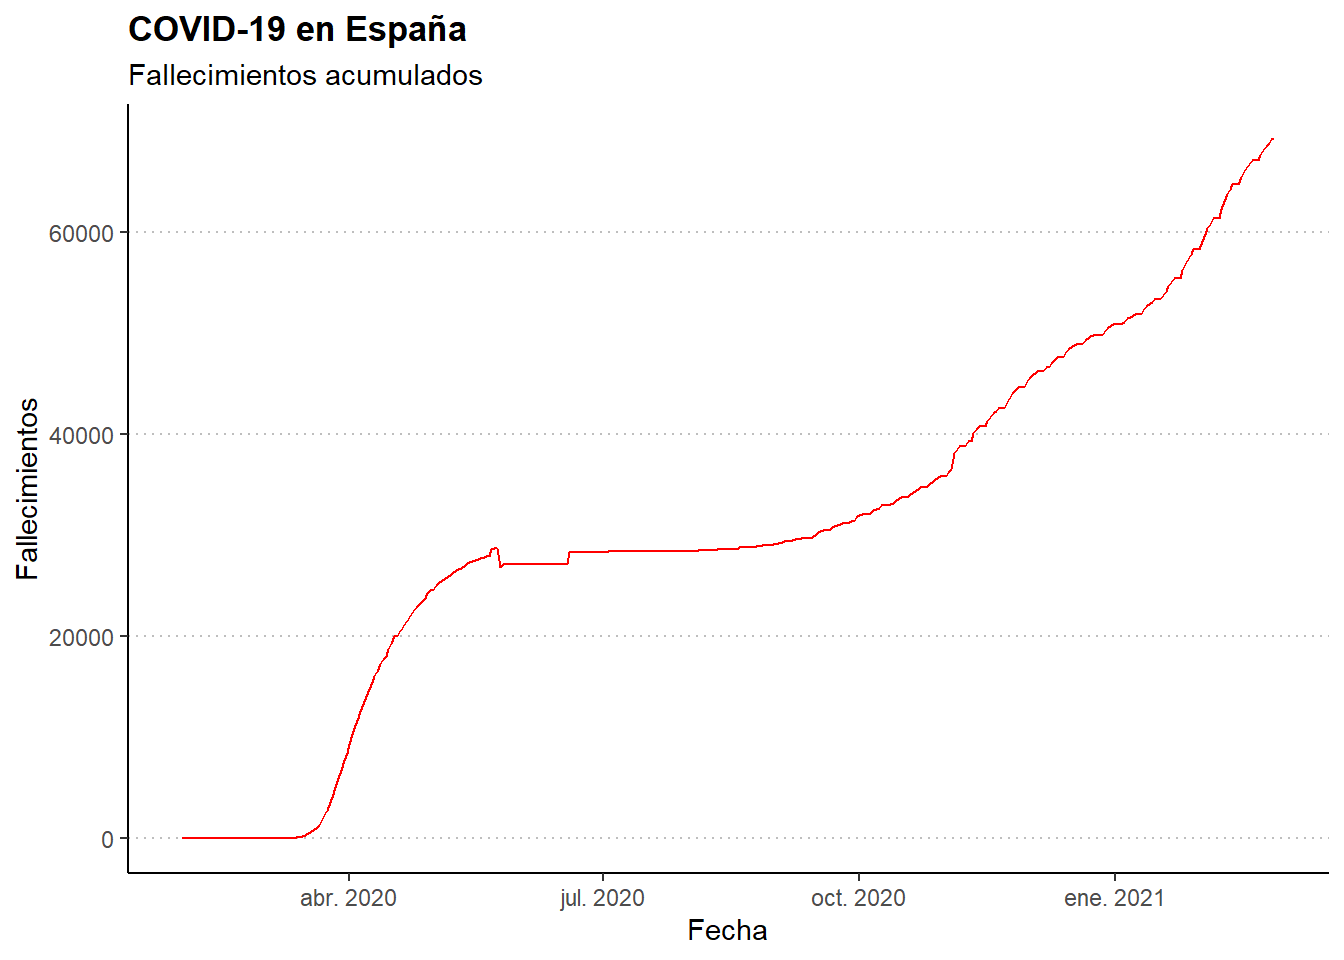
\includegraphics{book_LCC_files/figure-latex/unnamed-chunk-51-1.pdf}

\begin{Shaded}
\begin{Highlighting}[]
\NormalTok{g2 }\OtherTok{\textless{}{-}}\NormalTok{ datacovid\_por\_dia\_Spain }\SpecialCharTok{\%\textgreater{}\%}
    \FunctionTok{ggplot}\NormalTok{(}\FunctionTok{aes}\NormalTok{(}\AttributeTok{x=}\NormalTok{ObservationDate, }\AttributeTok{y=}\NormalTok{Confirmed)) }\SpecialCharTok{+}  \FunctionTok{geom\_line}\NormalTok{(}\AttributeTok{color =} \StringTok{"blue"}\NormalTok{) }\SpecialCharTok{+}\FunctionTok{ggtitle}\NormalTok{(}\StringTok{"COVID{-}19 en España"}\NormalTok{, }\AttributeTok{subtitle =} \StringTok{"Casos confirmados acumulados"}\NormalTok{)}\SpecialCharTok{+}\FunctionTok{theme}\NormalTok{(}\AttributeTok{plot.title =} \FunctionTok{element\_text}\NormalTok{(}\AttributeTok{face=}\StringTok{"bold"}\NormalTok{))}\SpecialCharTok{+}\FunctionTok{labs}\NormalTok{(}\AttributeTok{x=}\StringTok{"Fecha"}\NormalTok{, }\AttributeTok{y =}\StringTok{"Confirmados"}\NormalTok{)}\SpecialCharTok{+}\FunctionTok{theme}\NormalTok{(}\AttributeTok{axis.line.x =} \FunctionTok{element\_line}\NormalTok{(}\AttributeTok{color =} \StringTok{"black"}\NormalTok{))}\SpecialCharTok{+}\FunctionTok{theme}\NormalTok{(}\AttributeTok{axis.line.y =} \FunctionTok{element\_line}\NormalTok{(}\AttributeTok{color =} \StringTok{"black"}\NormalTok{))}\SpecialCharTok{+}\FunctionTok{theme}\NormalTok{(}\AttributeTok{panel.grid.major.y =} \FunctionTok{element\_line}\NormalTok{(}\AttributeTok{linetype =} \StringTok{"dotted"}\NormalTok{,}\AttributeTok{colour =} \StringTok{"grey"}\NormalTok{))}\SpecialCharTok{+}\FunctionTok{theme}\NormalTok{(}\AttributeTok{panel.background =} \FunctionTok{element\_rect}\NormalTok{(}\StringTok{"white"}\NormalTok{))}
\NormalTok{g2}
\end{Highlighting}
\end{Shaded}

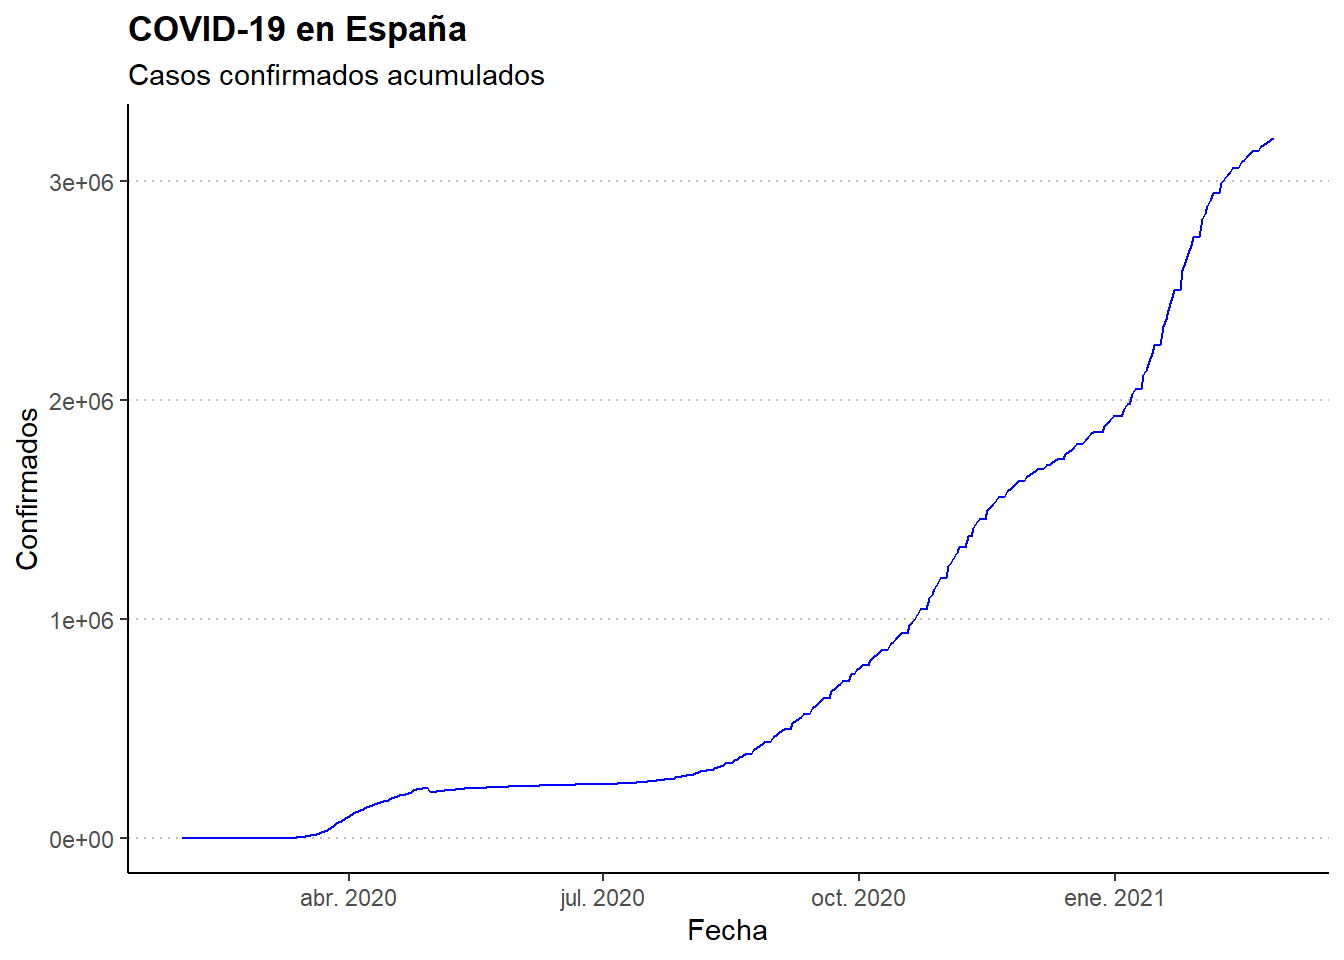
\includegraphics{book_LCC_files/figure-latex/unnamed-chunk-52-1.pdf}

\begin{Shaded}
\begin{Highlighting}[]
\NormalTok{g3 }\OtherTok{\textless{}{-}}\NormalTok{ datacovid\_por\_dia\_Spain }\SpecialCharTok{\%\textgreater{}\%}
    \FunctionTok{ggplot}\NormalTok{(}\FunctionTok{aes}\NormalTok{(}\AttributeTok{x=}\NormalTok{ObservationDate, }\AttributeTok{y=}\NormalTok{Recovered)) }\SpecialCharTok{+}  \FunctionTok{geom\_line}\NormalTok{(}\AttributeTok{color =} \StringTok{"green"}\NormalTok{) }\SpecialCharTok{+}\FunctionTok{ggtitle}\NormalTok{(}\StringTok{"COVID{-}19 en España"}\NormalTok{, }\AttributeTok{subtitle =} \StringTok{"Recuperados acumulados"}\NormalTok{)}\SpecialCharTok{+}\FunctionTok{theme}\NormalTok{(}\AttributeTok{plot.title =} \FunctionTok{element\_text}\NormalTok{(}\AttributeTok{face=}\StringTok{"bold"}\NormalTok{))}\SpecialCharTok{+}\FunctionTok{labs}\NormalTok{(}\AttributeTok{x=}\StringTok{"Fecha"}\NormalTok{, }\AttributeTok{y =}\StringTok{"Recuperados"}\NormalTok{)}\SpecialCharTok{+}\FunctionTok{theme}\NormalTok{(}\AttributeTok{axis.line.x =} \FunctionTok{element\_line}\NormalTok{(}\AttributeTok{color =} \StringTok{"black"}\NormalTok{))}\SpecialCharTok{+}\FunctionTok{theme}\NormalTok{(}\AttributeTok{axis.line.y =} \FunctionTok{element\_line}\NormalTok{(}\AttributeTok{color =} \StringTok{"black"}\NormalTok{))}\SpecialCharTok{+}\FunctionTok{theme}\NormalTok{(}\AttributeTok{panel.grid.major.y =} \FunctionTok{element\_line}\NormalTok{(}\AttributeTok{linetype =} \StringTok{"dotted"}\NormalTok{,}\AttributeTok{colour =} \StringTok{"grey"}\NormalTok{))}\SpecialCharTok{+}\FunctionTok{theme}\NormalTok{(}\AttributeTok{panel.background =} \FunctionTok{element\_rect}\NormalTok{(}\StringTok{"white"}\NormalTok{))}
\NormalTok{g3}
\end{Highlighting}
\end{Shaded}

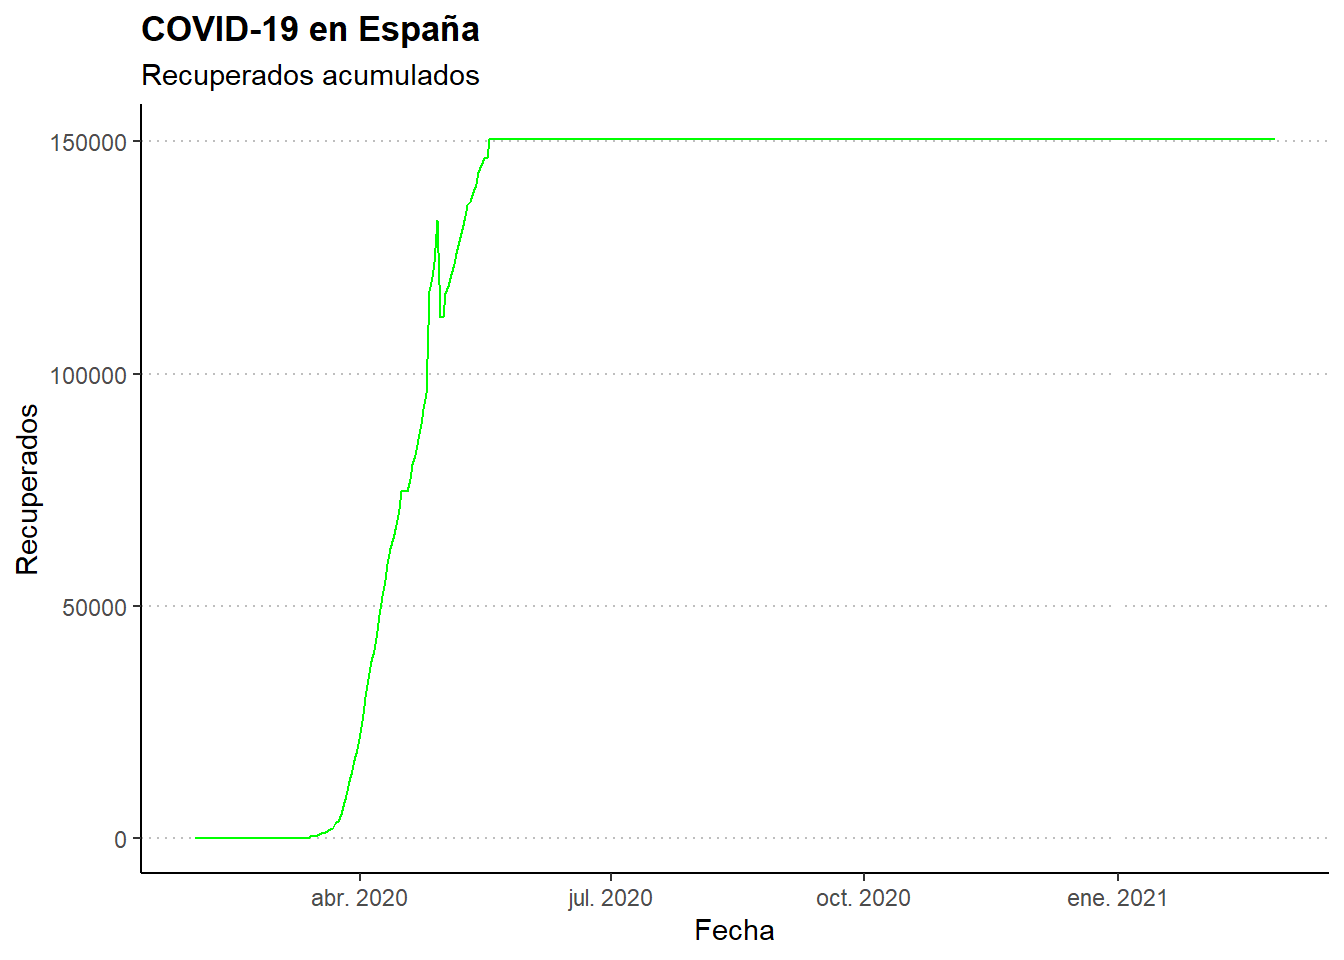
\includegraphics{book_LCC_files/figure-latex/unnamed-chunk-53-1.pdf}

Visualizar los casos acumulados en cada mes desde que comenzó la pandemia en China.

\begin{Shaded}
\begin{Highlighting}[]
\NormalTok{meses }\OtherTok{\textless{}{-}} \FunctionTok{month}\NormalTok{(}\FunctionTok{ymd}\NormalTok{(datacovid\_por\_dia\_Spain}\SpecialCharTok{$}\NormalTok{ObservationDate))}
\NormalTok{años }\OtherTok{\textless{}{-}} \FunctionTok{year}\NormalTok{(}\FunctionTok{ymd}\NormalTok{(datacovid\_por\_dia\_Spain}\SpecialCharTok{$}\NormalTok{ObservationDate))}
\NormalTok{ datacovid\_Spain\_fecha }\OtherTok{=}\NormalTok{ datacovid\_por\_dia\_Spain}
\NormalTok{ datacovid\_Spain\_fecha }\OtherTok{\textless{}{-}} \FunctionTok{mutate}\NormalTok{(datacovid\_Spain\_fecha, }\AttributeTok{Mes=}\NormalTok{meses, Año }\OtherTok{=}\NormalTok{ años)}
\NormalTok{ datacovid\_Spain\_fecha }\OtherTok{\textless{}{-}} \FunctionTok{unite}\NormalTok{(datacovid\_Spain\_fecha,Mes\_Año,}\FunctionTok{c}\NormalTok{(}\DecValTok{5}\SpecialCharTok{:}\DecValTok{6}\NormalTok{))}

\NormalTok{ datacovid\_Spain\_fecha }\OtherTok{\textless{}{-}}\NormalTok{ datacovid\_Spain\_fecha }\SpecialCharTok{\%\textgreater{}\%} \FunctionTok{group\_by}\NormalTok{(Mes\_Año) }\SpecialCharTok{\%\textgreater{}\%} \FunctionTok{summarise}\NormalTok{(}\AttributeTok{Confirmados=}\FunctionTok{max}\NormalTok{(Confirmed)) }\SpecialCharTok{\%\textgreater{}\%} \FunctionTok{arrange}\NormalTok{(Mes\_Año, Confirmados)}
 
\NormalTok{ g4 }\OtherTok{\textless{}{-}}\NormalTok{ datacovid\_Spain\_fecha }\SpecialCharTok{\%\textgreater{}\%}
     \FunctionTok{ggplot}\NormalTok{(}\FunctionTok{aes}\NormalTok{(}\AttributeTok{x=}\FunctionTok{reorder}\NormalTok{(Mes\_Año,Confirmados),}\AttributeTok{y=}\NormalTok{Confirmados,}\AttributeTok{fill=}\NormalTok{Confirmados)) }\SpecialCharTok{+}  \FunctionTok{geom\_bar}\NormalTok{(}\AttributeTok{stat =} \StringTok{"identity"}\NormalTok{) }\SpecialCharTok{+}\FunctionTok{ggtitle}\NormalTok{(}\StringTok{"COVID{-}19 en España"}\NormalTok{, }\AttributeTok{subtitle =} \StringTok{"Confirmados acumulados"}\NormalTok{)}\SpecialCharTok{+}\FunctionTok{theme}\NormalTok{(}\AttributeTok{plot.title =} \FunctionTok{element\_text}\NormalTok{(}\AttributeTok{face=}\StringTok{"bold"}\NormalTok{))}\SpecialCharTok{+}\FunctionTok{labs}\NormalTok{(}\AttributeTok{x=}\StringTok{"Mes\_Año"}\NormalTok{, }\AttributeTok{y =}\StringTok{"Confirmados"}\NormalTok{)}\SpecialCharTok{+}\FunctionTok{theme}\NormalTok{(}\AttributeTok{axis.line.x =} \FunctionTok{element\_line}\NormalTok{(}\AttributeTok{color =} \StringTok{"black"}\NormalTok{))}\SpecialCharTok{+}\FunctionTok{theme}\NormalTok{(}\AttributeTok{axis.line.y =} \FunctionTok{element\_line}\NormalTok{(}\AttributeTok{color =} \StringTok{"black"}\NormalTok{))}\SpecialCharTok{+}\FunctionTok{theme}\NormalTok{(}\AttributeTok{panel.grid.major.y =} \FunctionTok{element\_line}\NormalTok{(}\AttributeTok{linetype =} \StringTok{"dotted"}\NormalTok{,}\AttributeTok{colour =} \StringTok{"grey"}\NormalTok{))}\SpecialCharTok{+}\FunctionTok{theme}\NormalTok{(}\AttributeTok{panel.background =} \FunctionTok{element\_rect}\NormalTok{(}\StringTok{"white"}\NormalTok{))}\SpecialCharTok{+}\FunctionTok{scale\_fill\_gradient}\NormalTok{(}\AttributeTok{low =} \StringTok{"dark red"}\NormalTok{,}\AttributeTok{high =} \StringTok{"red"}\NormalTok{)}\SpecialCharTok{+}\FunctionTok{theme}\NormalTok{(}\AttributeTok{axis.text.x =} \FunctionTok{element\_text}\NormalTok{(}\AttributeTok{size =} \DecValTok{7}\NormalTok{,}\AttributeTok{hjust =} \FloatTok{0.6}\NormalTok{))}
\NormalTok{g4}
\end{Highlighting}
\end{Shaded}

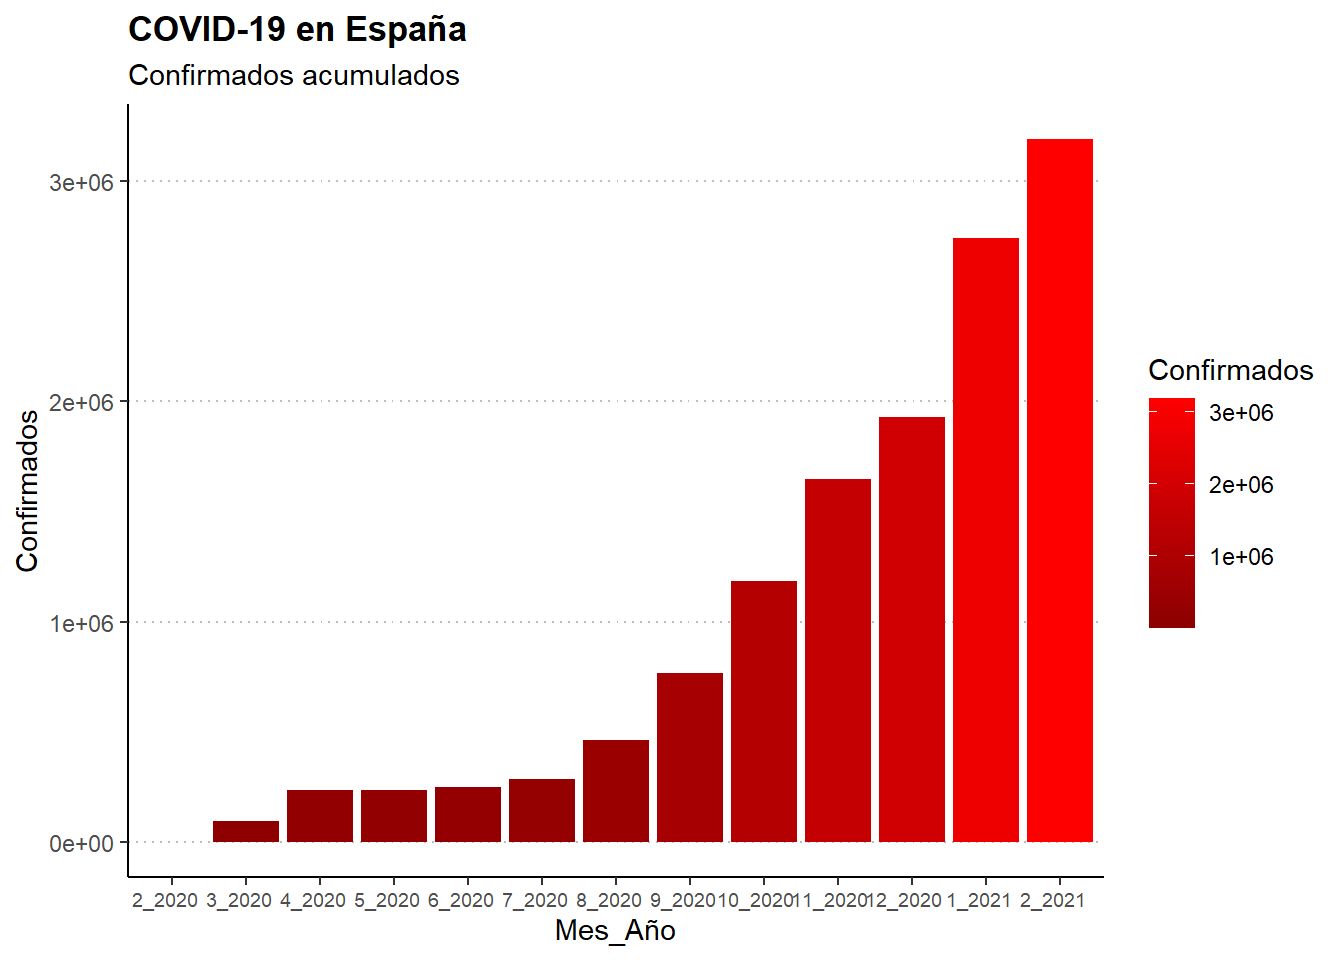
\includegraphics{book_LCC_files/figure-latex/unnamed-chunk-54-1.pdf}

Obtener una tabla con los los 20 paises con más fallecimientos y visualizar:

\begin{itemize}
\tightlist
\item
  Los fallecimientos acumulados, contagios acumulados y recuperaciones acumuladas para estos 20 paises
\item
  La evolución para estos 20 paises de los fallecimientos en la misma gráfica
\item
  La evolución para estos 20 paises de los contagios en la misma gráfica
\end{itemize}

\begin{Shaded}
\begin{Highlighting}[]
\NormalTok{paises\_mas\_fallecidos }\OtherTok{\textless{}{-}}\NormalTok{ datacovid\_por\_dia }\SpecialCharTok{\%\textgreater{}\%} \FunctionTok{group\_by}\NormalTok{(}\StringTok{\textasciigrave{}}\AttributeTok{Country/Region}\StringTok{\textasciigrave{}}\NormalTok{) }\SpecialCharTok{\%\textgreater{}\%}\FunctionTok{summarise}\NormalTok{(}\AttributeTok{Total\_Fallecidos=}\FunctionTok{max}\NormalTok{(Deaths), }\AttributeTok{Total\_Contagios=}\FunctionTok{max}\NormalTok{(Confirmed), }\AttributeTok{Total\_Recuperados=}\FunctionTok{max}\NormalTok{(Recovered)) }\SpecialCharTok{\%\textgreater{}\%} \FunctionTok{arrange}\NormalTok{(}\FunctionTok{desc}\NormalTok{(Total\_Fallecidos))}

\NormalTok{paises\_mas\_fallecidos }\OtherTok{\textless{}{-}}\NormalTok{ paises\_mas\_fallecidos[}\DecValTok{1}\SpecialCharTok{:}\DecValTok{20}\NormalTok{,]}

\NormalTok{paises\_mas\_fallecidos}
\end{Highlighting}
\end{Shaded}

\begin{verbatim}
## # A tibble: 20 x 4
##    `Country/Region` Total_Fallecidos Total_Contagios Total_Recuperados
##    <chr>                       <dbl>           <dbl>             <dbl>
##  1 US                         511994        28554465           6399531
##  2 Brazil                     254221        10517232           9371448
##  3 Mexico                     185257         2084128           1630002
##  4 India                      157051        11096731          10775169
##  5 UK                         122939         4182772             11602
##  6 Italy                       97507         2907825           2398352
##  7 France                      85741         3747263            261649
##  8 Russia                      84330         4187166           3756808
##  9 Germany                     70092         2444177           2252970
## 10 Spain                       69142         3188553            150376
## 11 Iran                        59980         1623159           1386534
## 12 Colombia                    59660         2248135           2145450
## 13 Argentina                   51946         2104197           1899087
## 14 South Africa                49941         1512225           1429047
## 15 Peru                        46299         1323863           1225995
## 16 Poland                      43656         1696885           1414461
## 17 Indonesia                   35981         1329074           1136054
## 18 Turkey                      28503         2693164           2565723
## 19 Ukraine                     27306         1389570           1210919
## 20 Belgium                     22052          769414             31130
\end{verbatim}

\begin{Shaded}
\begin{Highlighting}[]
\NormalTok{g5 }\OtherTok{\textless{}{-}}\NormalTok{ paises\_mas\_fallecidos }\SpecialCharTok{\%\textgreater{}\%}
    \FunctionTok{ggplot}\NormalTok{(}\FunctionTok{aes}\NormalTok{(}\AttributeTok{x=}\FunctionTok{reorder}\NormalTok{(}\StringTok{\textasciigrave{}}\AttributeTok{Country/Region}\StringTok{\textasciigrave{}}\NormalTok{,}\SpecialCharTok{{-}}\NormalTok{Total\_Fallecidos),}\AttributeTok{y=}\NormalTok{Total\_Fallecidos, }\AttributeTok{fill=}\NormalTok{Total\_Fallecidos)) }\SpecialCharTok{+}  \FunctionTok{geom\_bar}\NormalTok{(}\AttributeTok{stat =} \StringTok{"identity"}\NormalTok{) }\SpecialCharTok{+}\FunctionTok{ggtitle}\NormalTok{(}\StringTok{"COVID{-}19 en el Mundo"}\NormalTok{, }\AttributeTok{subtitle =} \StringTok{"Fallecidos acumulados"}\NormalTok{)}\SpecialCharTok{+}\FunctionTok{theme}\NormalTok{(}\AttributeTok{plot.title =} \FunctionTok{element\_text}\NormalTok{(}\AttributeTok{face=}\StringTok{"bold"}\NormalTok{))}\SpecialCharTok{+}\FunctionTok{labs}\NormalTok{(}\AttributeTok{x=}\StringTok{"Países"}\NormalTok{, }\AttributeTok{y =}\StringTok{"Fallecidos"}\NormalTok{)}\SpecialCharTok{+}\FunctionTok{theme}\NormalTok{(}\AttributeTok{axis.line.x =} \FunctionTok{element\_line}\NormalTok{(}\AttributeTok{color =} \StringTok{"black"}\NormalTok{))}\SpecialCharTok{+}\FunctionTok{theme}\NormalTok{(}\AttributeTok{axis.line.y =} \FunctionTok{element\_line}\NormalTok{(}\AttributeTok{color =} \StringTok{"black"}\NormalTok{))}\SpecialCharTok{+}\FunctionTok{theme}\NormalTok{(}\AttributeTok{panel.grid.major.y =} \FunctionTok{element\_line}\NormalTok{(}\AttributeTok{linetype =} \StringTok{"dotted"}\NormalTok{,}\AttributeTok{colour =} \StringTok{"grey"}\NormalTok{))}\SpecialCharTok{+}\FunctionTok{theme}\NormalTok{(}\AttributeTok{panel.background =} \FunctionTok{element\_rect}\NormalTok{(}\StringTok{"white"}\NormalTok{))}\SpecialCharTok{+}\FunctionTok{theme}\NormalTok{(}\AttributeTok{axis.text.x =} \FunctionTok{element\_text}\NormalTok{(}\AttributeTok{angle =} \DecValTok{90}\NormalTok{))}\SpecialCharTok{+}\FunctionTok{scale\_fill\_gradient}\NormalTok{(}\AttributeTok{low =} \StringTok{"orange"}\NormalTok{,}\AttributeTok{high =} \StringTok{"red"}\NormalTok{)}
\NormalTok{g5}
\end{Highlighting}
\end{Shaded}

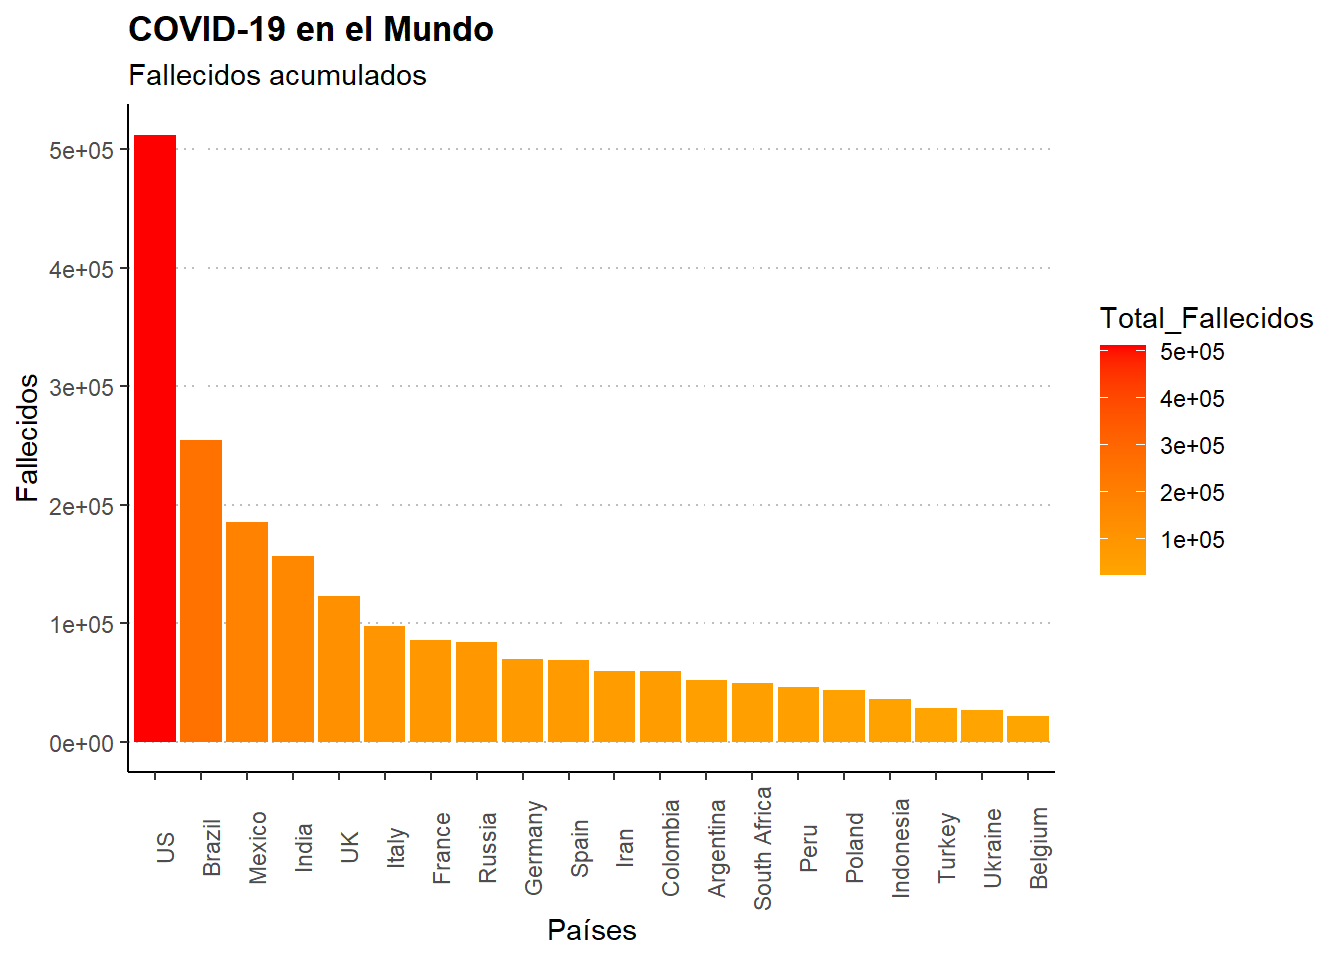
\includegraphics{book_LCC_files/figure-latex/unnamed-chunk-55-1.pdf}

\begin{Shaded}
\begin{Highlighting}[]
\NormalTok{g6 }\OtherTok{\textless{}{-}}\NormalTok{ paises\_mas\_fallecidos }\SpecialCharTok{\%\textgreater{}\%}
    \FunctionTok{ggplot}\NormalTok{(}\FunctionTok{aes}\NormalTok{(}\AttributeTok{x=}\FunctionTok{reorder}\NormalTok{(}\StringTok{\textasciigrave{}}\AttributeTok{Country/Region}\StringTok{\textasciigrave{}}\NormalTok{,}\SpecialCharTok{{-}}\NormalTok{Total\_Contagios),}\AttributeTok{y=}\NormalTok{Total\_Contagios, }\AttributeTok{fill=}\NormalTok{Total\_Contagios)) }\SpecialCharTok{+}  \FunctionTok{geom\_bar}\NormalTok{(}\AttributeTok{stat =} \StringTok{"identity"}\NormalTok{) }\SpecialCharTok{+}\FunctionTok{ggtitle}\NormalTok{(}\StringTok{"COVID{-}19 en el Mundo"}\NormalTok{, }\AttributeTok{subtitle =} \StringTok{"Contagios acumulados"}\NormalTok{)}\SpecialCharTok{+}\FunctionTok{theme}\NormalTok{(}\AttributeTok{plot.title =} \FunctionTok{element\_text}\NormalTok{(}\AttributeTok{face=}\StringTok{"bold"}\NormalTok{))}\SpecialCharTok{+}\FunctionTok{labs}\NormalTok{(}\AttributeTok{x=}\StringTok{"Países"}\NormalTok{, }\AttributeTok{y =}\StringTok{"Contagios"}\NormalTok{)}\SpecialCharTok{+}\FunctionTok{theme}\NormalTok{(}\AttributeTok{axis.line.x =} \FunctionTok{element\_line}\NormalTok{(}\AttributeTok{color =} \StringTok{"black"}\NormalTok{))}\SpecialCharTok{+}\FunctionTok{theme}\NormalTok{(}\AttributeTok{axis.line.y =} \FunctionTok{element\_line}\NormalTok{(}\AttributeTok{color =} \StringTok{"black"}\NormalTok{))}\SpecialCharTok{+}\FunctionTok{theme}\NormalTok{(}\AttributeTok{panel.grid.major.y =} \FunctionTok{element\_line}\NormalTok{(}\AttributeTok{linetype =} \StringTok{"dotted"}\NormalTok{,}\AttributeTok{colour =} \StringTok{"grey"}\NormalTok{))}\SpecialCharTok{+}\FunctionTok{theme}\NormalTok{(}\AttributeTok{panel.background =} \FunctionTok{element\_rect}\NormalTok{(}\StringTok{"white"}\NormalTok{))}\SpecialCharTok{+}\FunctionTok{theme}\NormalTok{(}\AttributeTok{axis.text.x =} \FunctionTok{element\_text}\NormalTok{(}\AttributeTok{angle =} \DecValTok{90}\NormalTok{))}
\NormalTok{g6}
\end{Highlighting}
\end{Shaded}

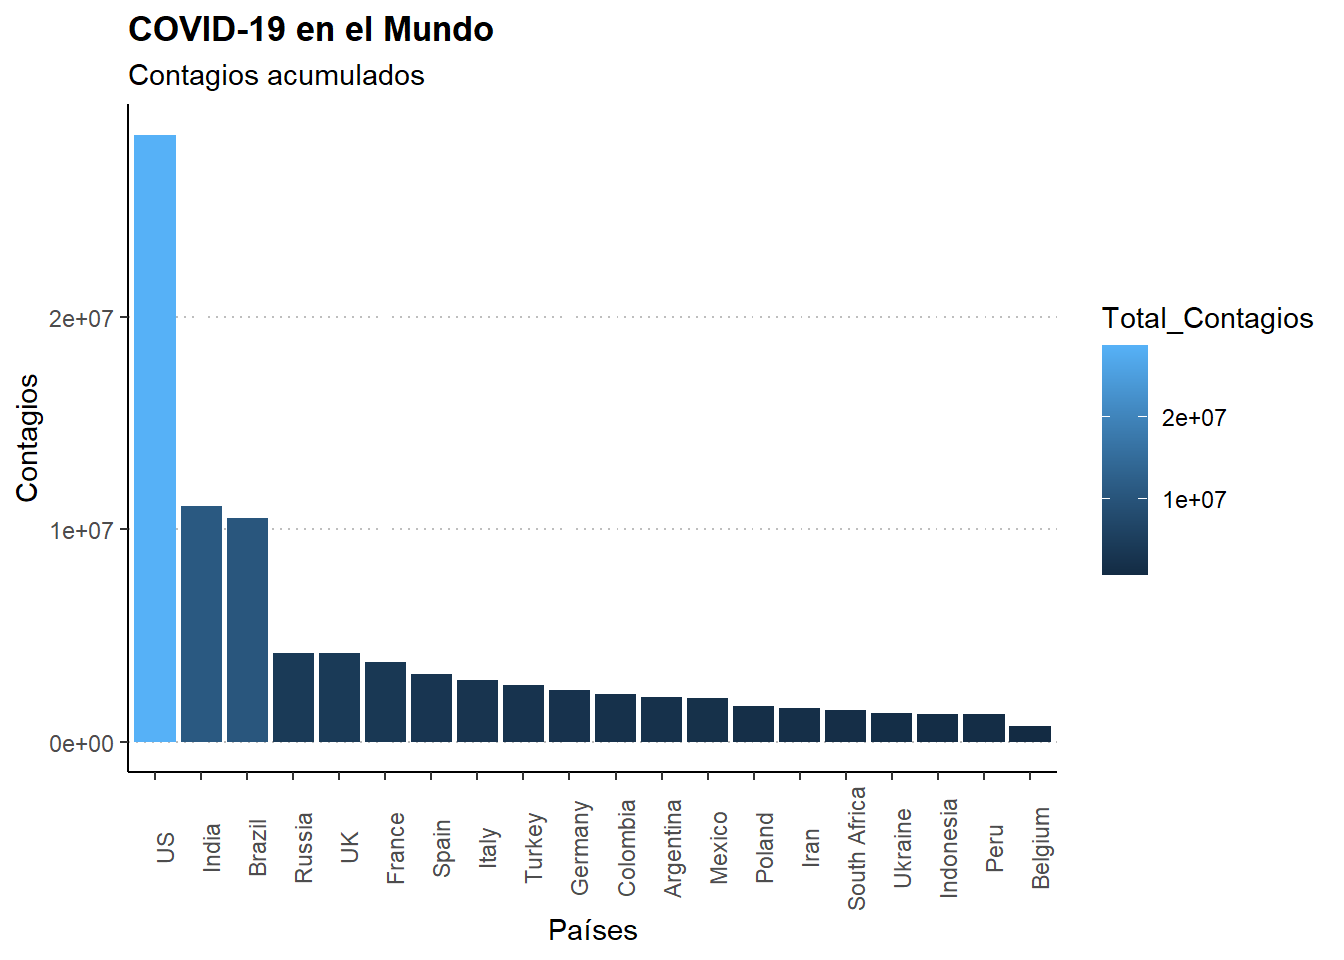
\includegraphics{book_LCC_files/figure-latex/unnamed-chunk-56-1.pdf}

\begin{Shaded}
\begin{Highlighting}[]
\NormalTok{g7 }\OtherTok{\textless{}{-}}\NormalTok{ paises\_mas\_fallecidos }\SpecialCharTok{\%\textgreater{}\%}
    \FunctionTok{ggplot}\NormalTok{(}\FunctionTok{aes}\NormalTok{(}\AttributeTok{x=}\FunctionTok{reorder}\NormalTok{(}\StringTok{\textasciigrave{}}\AttributeTok{Country/Region}\StringTok{\textasciigrave{}}\NormalTok{,}\SpecialCharTok{{-}}\NormalTok{Total\_Recuperados),}\AttributeTok{y=}\NormalTok{Total\_Recuperados, }\AttributeTok{fill=}\NormalTok{Total\_Recuperados)) }\SpecialCharTok{+}  \FunctionTok{geom\_bar}\NormalTok{(}\AttributeTok{stat =} \StringTok{"identity"}\NormalTok{) }\SpecialCharTok{+}\FunctionTok{ggtitle}\NormalTok{(}\StringTok{"COVID{-}19 en el Mundo"}\NormalTok{, }\AttributeTok{subtitle =} \StringTok{"Recuperados acumulados"}\NormalTok{)}\SpecialCharTok{+}\FunctionTok{theme}\NormalTok{(}\AttributeTok{plot.title =} \FunctionTok{element\_text}\NormalTok{(}\AttributeTok{face=}\StringTok{"bold"}\NormalTok{))}\SpecialCharTok{+}\FunctionTok{labs}\NormalTok{(}\AttributeTok{x=}\StringTok{"Países"}\NormalTok{, }\AttributeTok{y =}\StringTok{"Recuperados"}\NormalTok{)}\SpecialCharTok{+}\FunctionTok{theme}\NormalTok{(}\AttributeTok{axis.line.x =} \FunctionTok{element\_line}\NormalTok{(}\AttributeTok{color =} \StringTok{"black"}\NormalTok{))}\SpecialCharTok{+}\FunctionTok{theme}\NormalTok{(}\AttributeTok{axis.line.y =} \FunctionTok{element\_line}\NormalTok{(}\AttributeTok{color =} \StringTok{"black"}\NormalTok{))}\SpecialCharTok{+}\FunctionTok{theme}\NormalTok{(}\AttributeTok{panel.grid.major.y =} \FunctionTok{element\_line}\NormalTok{(}\AttributeTok{linetype =} \StringTok{"dotted"}\NormalTok{,}\AttributeTok{colour =} \StringTok{"grey"}\NormalTok{))}\SpecialCharTok{+}\FunctionTok{theme}\NormalTok{(}\AttributeTok{panel.background =} \FunctionTok{element\_rect}\NormalTok{(}\StringTok{"white"}\NormalTok{))}\SpecialCharTok{+}\FunctionTok{theme}\NormalTok{(}\AttributeTok{axis.text.x =} \FunctionTok{element\_text}\NormalTok{(}\AttributeTok{angle =} \DecValTok{90}\NormalTok{))}\SpecialCharTok{+}\FunctionTok{scale\_fill\_gradient}\NormalTok{(}\AttributeTok{low =} \StringTok{"dark green"}\NormalTok{,}\AttributeTok{high =} \StringTok{"light green"}\NormalTok{)}
\NormalTok{g7}
\end{Highlighting}
\end{Shaded}

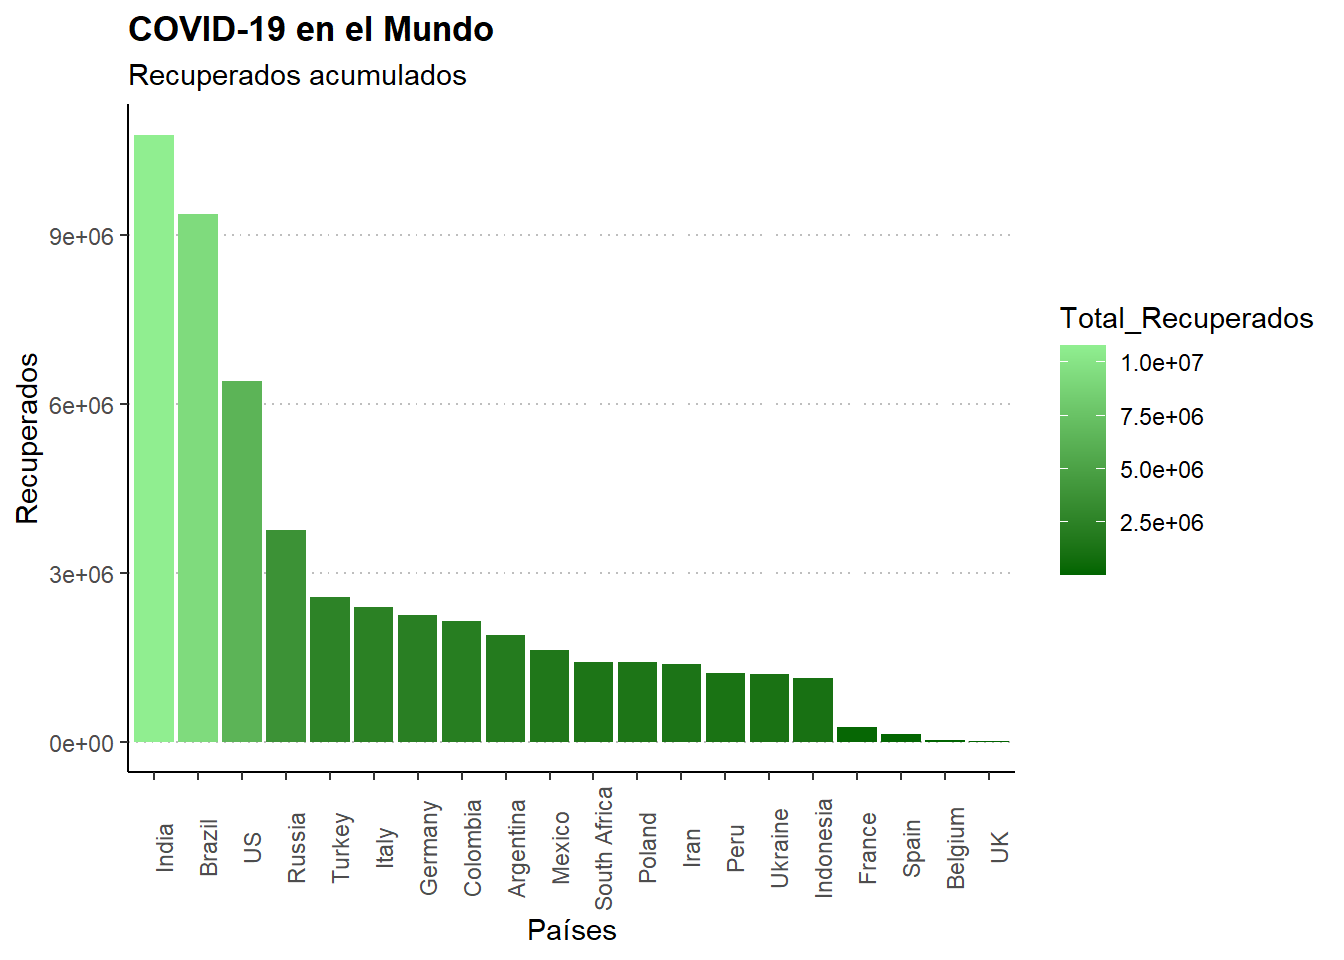
\includegraphics{book_LCC_files/figure-latex/unnamed-chunk-57-1.pdf}

\begin{Shaded}
\begin{Highlighting}[]
\NormalTok{covid\_top20 }\OtherTok{\textless{}{-}}\NormalTok{ covid\_19\_data }\SpecialCharTok{\%\textgreater{}\%}\FunctionTok{filter}\NormalTok{(}\StringTok{\textasciigrave{}}\AttributeTok{Country/Region}\StringTok{\textasciigrave{}}\SpecialCharTok{==}\NormalTok{paises\_mas\_fallecidos}\SpecialCharTok{$}\StringTok{\textasciigrave{}}\AttributeTok{Country/Region}\StringTok{\textasciigrave{}}\NormalTok{) }\SpecialCharTok{\%\textgreater{}\%} \FunctionTok{group\_by}\NormalTok{(}\StringTok{\textasciigrave{}}\AttributeTok{Country/Region}\StringTok{\textasciigrave{}}\NormalTok{,ObservationDate) }\SpecialCharTok{\%\textgreater{}\%} \FunctionTok{summarise}\NormalTok{(}\AttributeTok{Confirmed=}\FunctionTok{sum}\NormalTok{(Confirmed),}\AttributeTok{Deaths=}\FunctionTok{sum}\NormalTok{(Deaths), }\AttributeTok{Recovered =} \FunctionTok{sum}\NormalTok{(Recovered))}
\end{Highlighting}
\end{Shaded}

\begin{verbatim}
## `summarise()` has grouped output by 'Country/Region'. You can override using the `.groups` argument.
\end{verbatim}

\begin{Shaded}
\begin{Highlighting}[]
\NormalTok{covid\_top20}\SpecialCharTok{$}\NormalTok{ObservationDate}\OtherTok{\textless{}{-}} \FunctionTok{as.Date}\NormalTok{(covid\_top20}\SpecialCharTok{$}\NormalTok{ObservationDate,}\AttributeTok{format=}\StringTok{"\%m/\%d/\%Y"}\NormalTok{)}

\NormalTok{g8 }\OtherTok{\textless{}{-}}\NormalTok{ covid\_top20 }\SpecialCharTok{\%\textgreater{}\%}
    \FunctionTok{ggplot}\NormalTok{(}\FunctionTok{aes}\NormalTok{(}\AttributeTok{x=}\NormalTok{ObservationDate, }\AttributeTok{y=}\NormalTok{Deaths,}\AttributeTok{group=}\StringTok{\textasciigrave{}}\AttributeTok{Country/Region}\StringTok{\textasciigrave{}}\NormalTok{)) }\SpecialCharTok{+}  \FunctionTok{geom\_line}\NormalTok{() }\SpecialCharTok{+}\FunctionTok{ggtitle}\NormalTok{(}\StringTok{"COVID{-}19 en el Mundo"}\NormalTok{, }\AttributeTok{subtitle =} \StringTok{"Evolución de fallecimientos por país"}\NormalTok{)}\SpecialCharTok{+}\FunctionTok{theme}\NormalTok{(}\AttributeTok{plot.title =} \FunctionTok{element\_text}\NormalTok{(}\AttributeTok{face=}\StringTok{"bold"}\NormalTok{))}\SpecialCharTok{+}\FunctionTok{labs}\NormalTok{(}\AttributeTok{x=}\StringTok{"Fecha"}\NormalTok{, }\AttributeTok{y =}\StringTok{"Fallecimientos"}\NormalTok{)}\SpecialCharTok{+}\FunctionTok{theme}\NormalTok{(}\AttributeTok{axis.line.x =} \FunctionTok{element\_line}\NormalTok{(}\AttributeTok{color =} \StringTok{"black"}\NormalTok{))}\SpecialCharTok{+}\FunctionTok{theme}\NormalTok{(}\AttributeTok{axis.line.y =} \FunctionTok{element\_line}\NormalTok{(}\AttributeTok{color =} \StringTok{"black"}\NormalTok{))}\SpecialCharTok{+}\FunctionTok{theme}\NormalTok{(}\AttributeTok{panel.grid.major.y =} \FunctionTok{element\_line}\NormalTok{(}\AttributeTok{linetype =} \StringTok{"dotted"}\NormalTok{,}\AttributeTok{colour =} \StringTok{"grey"}\NormalTok{))}\SpecialCharTok{+}\FunctionTok{theme}\NormalTok{(}\AttributeTok{panel.background =} \FunctionTok{element\_rect}\NormalTok{(}\StringTok{"white"}\NormalTok{))}\SpecialCharTok{+}\FunctionTok{theme}\NormalTok{(}\AttributeTok{axis.text.x =} \FunctionTok{element\_text}\NormalTok{(}\AttributeTok{angle =} \DecValTok{90}\NormalTok{))}

\NormalTok{g8 }\OtherTok{\textless{}{-}}\NormalTok{ g8 }\SpecialCharTok{+} \FunctionTok{geom\_line}\NormalTok{(}\AttributeTok{color=}\StringTok{"red"}\NormalTok{) }\SpecialCharTok{+} \FunctionTok{facet\_wrap}\NormalTok{(}\SpecialCharTok{\textasciitilde{}}\StringTok{\textasciigrave{}}\AttributeTok{Country/Region}\StringTok{\textasciigrave{}}\NormalTok{, }\AttributeTok{ncol =} \DecValTok{5}\NormalTok{)}
\NormalTok{g8}
\end{Highlighting}
\end{Shaded}

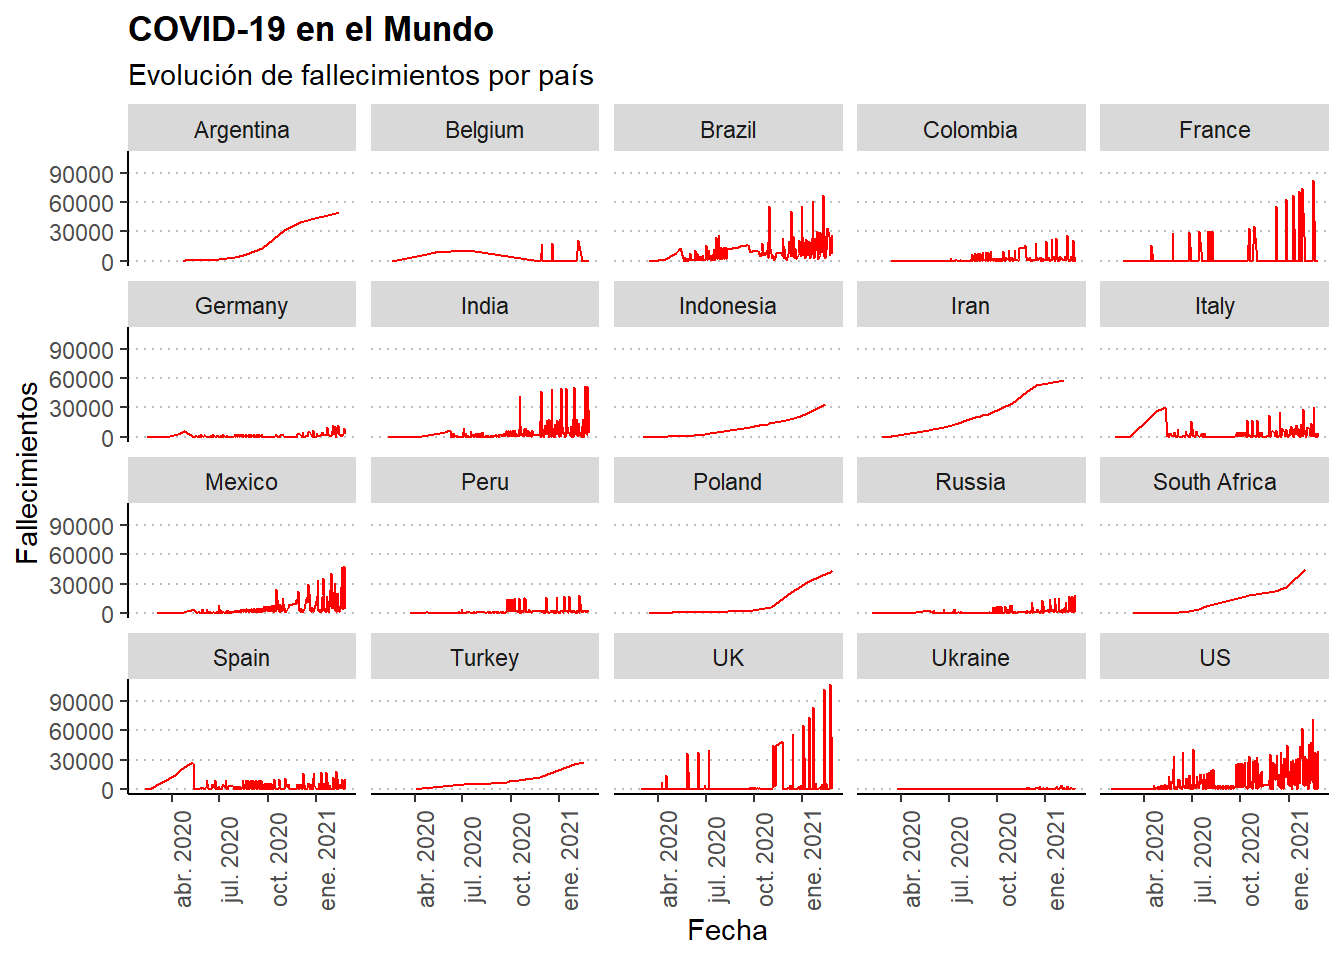
\includegraphics{book_LCC_files/figure-latex/unnamed-chunk-58-1.pdf}

\begin{Shaded}
\begin{Highlighting}[]
\NormalTok{g9 }\OtherTok{\textless{}{-}}\NormalTok{ covid\_top20 }\SpecialCharTok{\%\textgreater{}\%}
    \FunctionTok{ggplot}\NormalTok{(}\FunctionTok{aes}\NormalTok{(}\AttributeTok{x=}\NormalTok{ObservationDate, }\AttributeTok{y=}\NormalTok{Confirmed,}\AttributeTok{group=}\StringTok{\textasciigrave{}}\AttributeTok{Country/Region}\StringTok{\textasciigrave{}}\NormalTok{)) }\SpecialCharTok{+}  \FunctionTok{geom\_line}\NormalTok{() }\SpecialCharTok{+}\FunctionTok{ggtitle}\NormalTok{(}\StringTok{"COVID{-}19 en el Mundo"}\NormalTok{, }\AttributeTok{subtitle =} \StringTok{"Evolución de contagios por país"}\NormalTok{)}\SpecialCharTok{+}\FunctionTok{theme}\NormalTok{(}\AttributeTok{plot.title =} \FunctionTok{element\_text}\NormalTok{(}\AttributeTok{face=}\StringTok{"bold"}\NormalTok{))}\SpecialCharTok{+}\FunctionTok{labs}\NormalTok{(}\AttributeTok{x=}\StringTok{"Fecha"}\NormalTok{, }\AttributeTok{y =}\StringTok{"Contagios"}\NormalTok{)}\SpecialCharTok{+}\FunctionTok{theme}\NormalTok{(}\AttributeTok{axis.line.x =} \FunctionTok{element\_line}\NormalTok{(}\AttributeTok{color =} \StringTok{"black"}\NormalTok{))}\SpecialCharTok{+}\FunctionTok{theme}\NormalTok{(}\AttributeTok{axis.line.y =} \FunctionTok{element\_line}\NormalTok{(}\AttributeTok{color =} \StringTok{"black"}\NormalTok{))}\SpecialCharTok{+}\FunctionTok{theme}\NormalTok{(}\AttributeTok{panel.grid.major.y =} \FunctionTok{element\_line}\NormalTok{(}\AttributeTok{linetype =} \StringTok{"dotted"}\NormalTok{,}\AttributeTok{colour =} \StringTok{"grey"}\NormalTok{))}\SpecialCharTok{+}\FunctionTok{theme}\NormalTok{(}\AttributeTok{panel.background =} \FunctionTok{element\_rect}\NormalTok{(}\StringTok{"white"}\NormalTok{))}\SpecialCharTok{+}\FunctionTok{theme}\NormalTok{(}\AttributeTok{axis.text.x =} \FunctionTok{element\_text}\NormalTok{(}\AttributeTok{angle =} \DecValTok{90}\NormalTok{))}

\NormalTok{g9 }\OtherTok{\textless{}{-}}\NormalTok{ g9 }\SpecialCharTok{+} \FunctionTok{geom\_line}\NormalTok{(}\AttributeTok{color=}\StringTok{"blue"}\NormalTok{) }\SpecialCharTok{+} \FunctionTok{facet\_wrap}\NormalTok{(}\SpecialCharTok{\textasciitilde{}}\StringTok{\textasciigrave{}}\AttributeTok{Country/Region}\StringTok{\textasciigrave{}}\NormalTok{, }\AttributeTok{ncol =} \DecValTok{5}\NormalTok{ )}
\NormalTok{g9}
\end{Highlighting}
\end{Shaded}

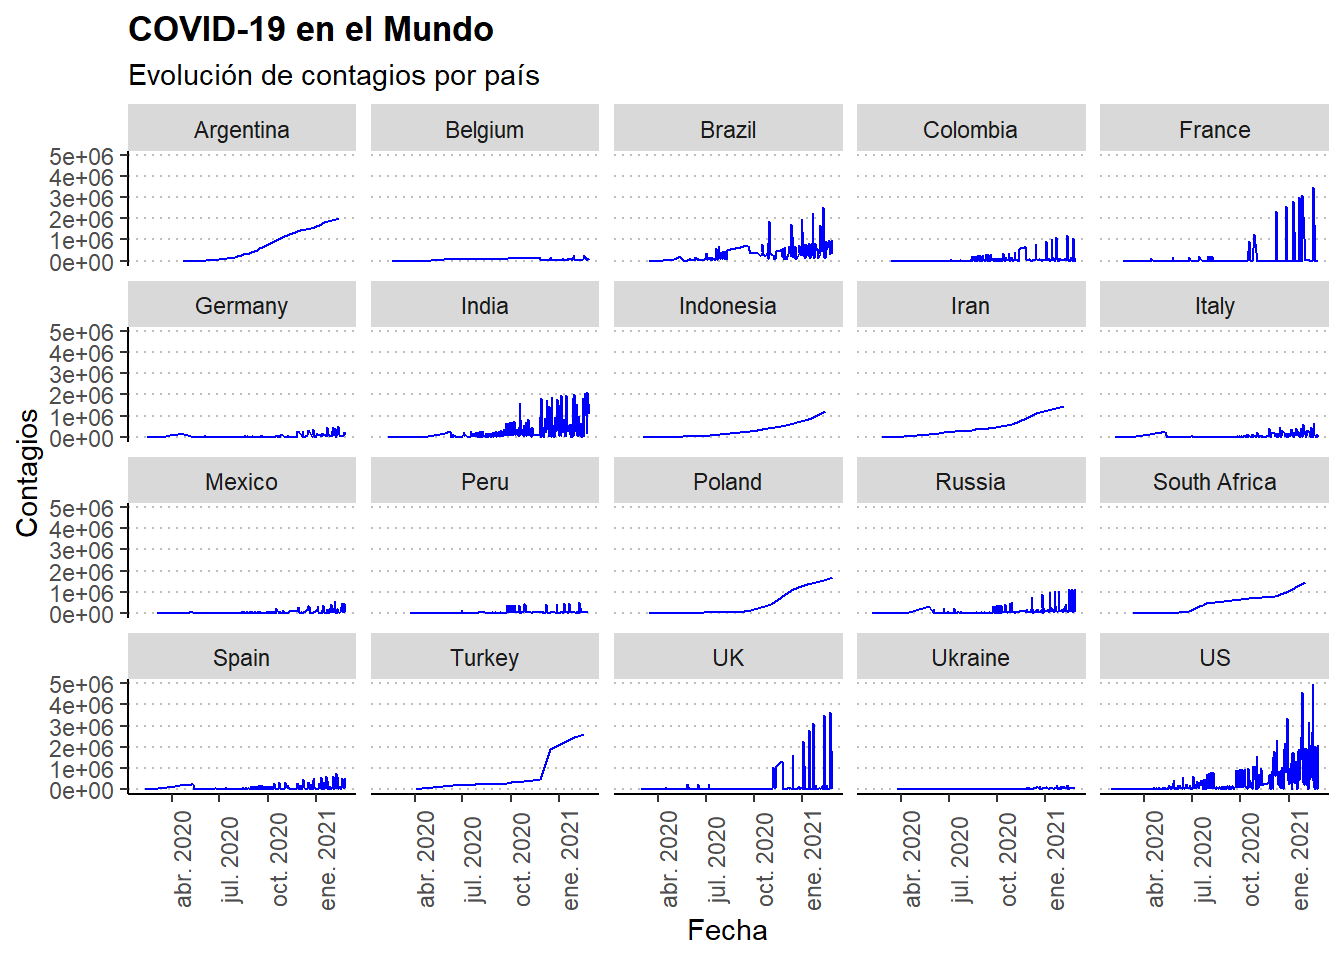
\includegraphics{book_LCC_files/figure-latex/unnamed-chunk-59-1.pdf}

COVID-19 en Andalucía

\begin{Shaded}
\begin{Highlighting}[]
\NormalTok{datacovid\_Andalucia }\OtherTok{\textless{}{-}}\NormalTok{ covid\_19\_data }\SpecialCharTok{\%\textgreater{}\%}          \FunctionTok{filter}\NormalTok{(covid\_19\_data[}\StringTok{\textquotesingle{}Country/Region\textquotesingle{}}\NormalTok{]}\SpecialCharTok{==}\StringTok{"Spain"}\NormalTok{, }\StringTok{\textasciigrave{}}\AttributeTok{Province/State}\StringTok{\textasciigrave{}}\SpecialCharTok{==}\StringTok{"Andalusia"}\NormalTok{) }\SpecialCharTok{\%\textgreater{}\%} \FunctionTok{select}\NormalTok{(ObservationDate,}\StringTok{\textasciigrave{}}\AttributeTok{Province/State}\StringTok{\textasciigrave{}}\NormalTok{,Confirmed,Deaths,Recovered) }

\NormalTok{datacovid\_Andalucia}\SpecialCharTok{$}\NormalTok{ObservationDate}\OtherTok{\textless{}{-}} \FunctionTok{as.Date}\NormalTok{(datacovid\_Andalucia}\SpecialCharTok{$}\NormalTok{ObservationDate,}\AttributeTok{format=}\StringTok{"\%m/\%d/\%Y"}\NormalTok{)}

\NormalTok{datacovid\_Andalucia}\OtherTok{\textless{}{-}}\NormalTok{ datacovid\_Andalucia }\SpecialCharTok{\%\textgreater{}\%} \FunctionTok{group\_by}\NormalTok{(ObservationDate) }\SpecialCharTok{\%\textgreater{}\%} \FunctionTok{summarise}\NormalTok{(}\AttributeTok{Confirmed=}\FunctionTok{sum}\NormalTok{(Confirmed), }\AttributeTok{Deaths=}\FunctionTok{sum}\NormalTok{(Deaths), }\AttributeTok{Recovered=}\FunctionTok{sum}\NormalTok{(Recovered))}

\NormalTok{meses\_andalucia }\OtherTok{\textless{}{-}} \FunctionTok{month}\NormalTok{(}\FunctionTok{ymd}\NormalTok{(datacovid\_Andalucia}\SpecialCharTok{$}\NormalTok{ObservationDate))}
\NormalTok{años\_andalucia }\OtherTok{\textless{}{-}} \FunctionTok{year}\NormalTok{(}\FunctionTok{ymd}\NormalTok{(datacovid\_Andalucia}\SpecialCharTok{$}\NormalTok{ObservationDate))}

\NormalTok{ datacovid\_Andalucia }\OtherTok{\textless{}{-}} \FunctionTok{mutate}\NormalTok{(datacovid\_Andalucia, }\AttributeTok{Mes=}\NormalTok{meses\_andalucia, Año }\OtherTok{=}\NormalTok{ años\_andalucia)}
\NormalTok{ datacovid\_Andalucia }\OtherTok{\textless{}{-}} \FunctionTok{unite}\NormalTok{(datacovid\_Andalucia,Mes\_Año,}\FunctionTok{c}\NormalTok{(}\DecValTok{5}\SpecialCharTok{:}\DecValTok{6}\NormalTok{))}

\NormalTok{ datacovid\_Andalucia }\OtherTok{\textless{}{-}}\NormalTok{ datacovid\_Andalucia }\SpecialCharTok{\%\textgreater{}\%} \FunctionTok{group\_by}\NormalTok{(Mes\_Año) }\SpecialCharTok{\%\textgreater{}\%} \FunctionTok{summarise}\NormalTok{(}\AttributeTok{Confirmados=}\FunctionTok{max}\NormalTok{(Confirmed)) }\SpecialCharTok{\%\textgreater{}\%} \FunctionTok{arrange}\NormalTok{(Mes\_Año, Confirmados)}
 
\NormalTok{ g10 }\OtherTok{\textless{}{-}}\NormalTok{ datacovid\_Andalucia }\SpecialCharTok{\%\textgreater{}\%}
     \FunctionTok{ggplot}\NormalTok{(}\FunctionTok{aes}\NormalTok{(}\AttributeTok{x=}\FunctionTok{reorder}\NormalTok{(Mes\_Año,Confirmados),}\AttributeTok{y=}\NormalTok{Confirmados,}\AttributeTok{fill=}\NormalTok{Confirmados)) }\SpecialCharTok{+}  \FunctionTok{geom\_bar}\NormalTok{(}\AttributeTok{stat =} \StringTok{"identity"}\NormalTok{) }\SpecialCharTok{+}\FunctionTok{ggtitle}\NormalTok{(}\StringTok{"COVID{-}19 en Andalucía"}\NormalTok{, }\AttributeTok{subtitle =} \StringTok{"Confirmados acumulados"}\NormalTok{)}\SpecialCharTok{+}\FunctionTok{theme}\NormalTok{(}\AttributeTok{plot.title =} \FunctionTok{element\_text}\NormalTok{(}\AttributeTok{face=}\StringTok{"bold"}\NormalTok{))}\SpecialCharTok{+}\FunctionTok{labs}\NormalTok{(}\AttributeTok{x=}\StringTok{"Mes\_Año"}\NormalTok{, }\AttributeTok{y =}\StringTok{"Confirmados"}\NormalTok{)}\SpecialCharTok{+}\FunctionTok{theme}\NormalTok{(}\AttributeTok{axis.line.x =} \FunctionTok{element\_line}\NormalTok{(}\AttributeTok{color =} \StringTok{"black"}\NormalTok{))}\SpecialCharTok{+}\FunctionTok{theme}\NormalTok{(}\AttributeTok{axis.line.y =} \FunctionTok{element\_line}\NormalTok{(}\AttributeTok{color =} \StringTok{"black"}\NormalTok{))}\SpecialCharTok{+}\FunctionTok{theme}\NormalTok{(}\AttributeTok{panel.grid.major.y =} \FunctionTok{element\_line}\NormalTok{(}\AttributeTok{linetype =} \StringTok{"dotted"}\NormalTok{,}\AttributeTok{colour =} \StringTok{"grey"}\NormalTok{))}\SpecialCharTok{+}\FunctionTok{theme}\NormalTok{(}\AttributeTok{panel.background =} \FunctionTok{element\_rect}\NormalTok{(}\StringTok{"white"}\NormalTok{))}\SpecialCharTok{+}\FunctionTok{scale\_fill\_gradient}\NormalTok{(}\AttributeTok{low =} \StringTok{"dark red"}\NormalTok{,}\AttributeTok{high =} \StringTok{"red"}\NormalTok{)}\SpecialCharTok{+}\FunctionTok{theme}\NormalTok{(}\AttributeTok{axis.text.x =} \FunctionTok{element\_text}\NormalTok{(}\AttributeTok{size =} \DecValTok{7}\NormalTok{,}\AttributeTok{hjust =} \FloatTok{0.6}\NormalTok{))}
\NormalTok{g10}
\end{Highlighting}
\end{Shaded}

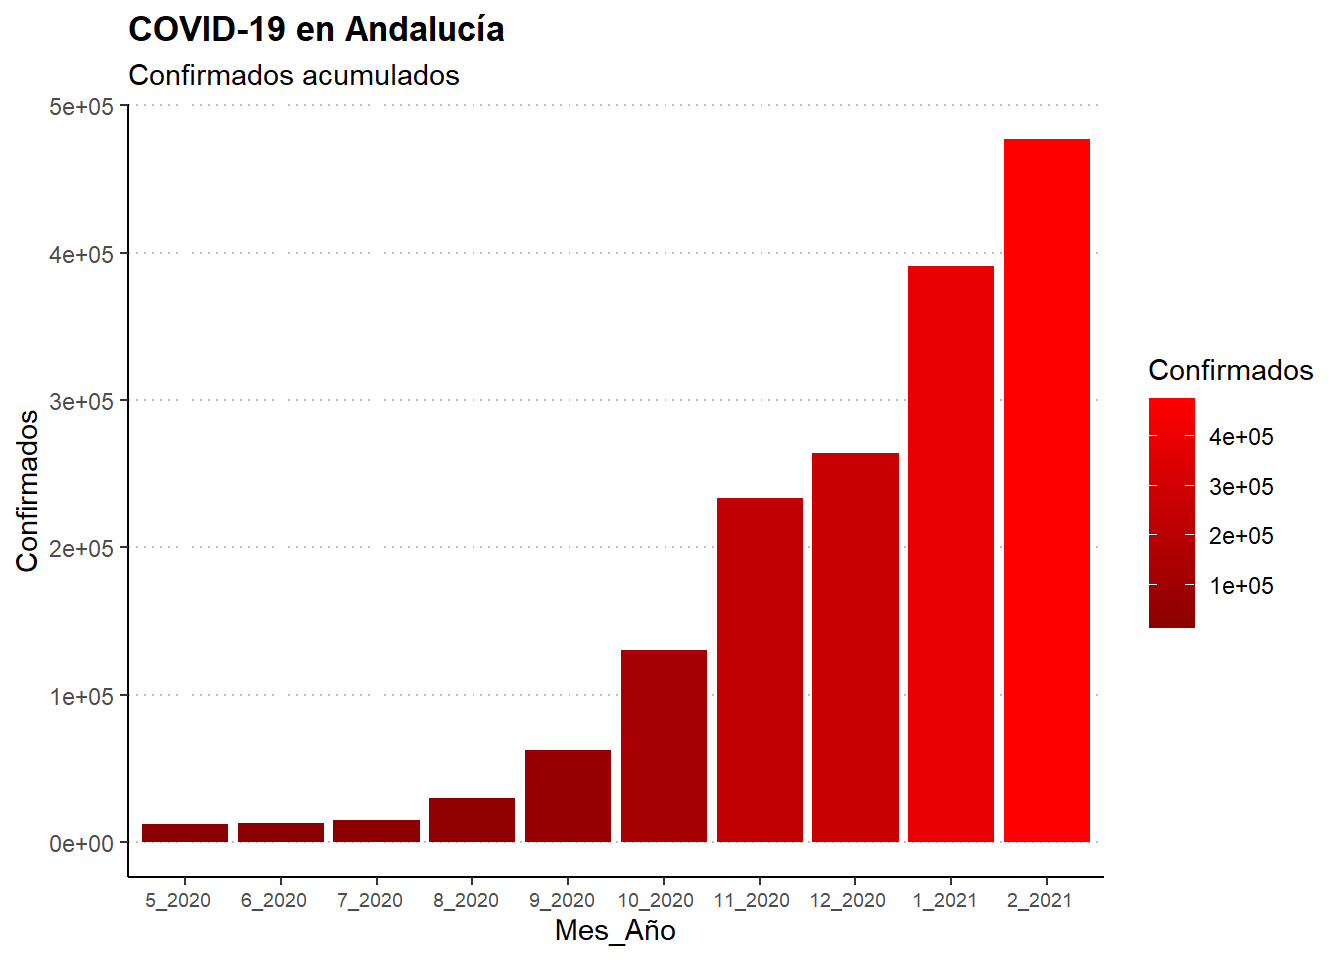
\includegraphics{book_LCC_files/figure-latex/unnamed-chunk-60-1.pdf}

Evolución de casos confirmados COVID-19 Andalucía

\begin{Shaded}
\begin{Highlighting}[]
\NormalTok{datacovid\_por\_dia\_Andalucia }\OtherTok{\textless{}{-}}\NormalTok{ covid\_19\_data }\SpecialCharTok{\%\textgreater{}\%}          \FunctionTok{filter}\NormalTok{(covid\_19\_data[}\StringTok{\textquotesingle{}Country/Region\textquotesingle{}}\NormalTok{]}\SpecialCharTok{==}\StringTok{"Spain"}\NormalTok{, }\StringTok{\textasciigrave{}}\AttributeTok{Province/State}\StringTok{\textasciigrave{}}\SpecialCharTok{==}\StringTok{"Andalusia"}\NormalTok{) }\SpecialCharTok{\%\textgreater{}\%} \FunctionTok{select}\NormalTok{(ObservationDate,Confirmed,Deaths,Recovered) }

\NormalTok{datacovid\_por\_dia\_Andalucia}\SpecialCharTok{$}\NormalTok{ObservationDate}\OtherTok{\textless{}{-}} \FunctionTok{as.Date}\NormalTok{(datacovid\_por\_dia\_Andalucia}\SpecialCharTok{$}\NormalTok{ObservationDate,}\AttributeTok{format=}\StringTok{"\%m/\%d/\%Y"}\NormalTok{)}

\NormalTok{datacovid\_por\_dia\_Andalucia}\OtherTok{\textless{}{-}}\NormalTok{ datacovid\_por\_dia\_Andalucia }\SpecialCharTok{\%\textgreater{}\%} \FunctionTok{group\_by}\NormalTok{(ObservationDate) }\SpecialCharTok{\%\textgreater{}\%} \FunctionTok{summarise}\NormalTok{(}\AttributeTok{Confirmed=}\FunctionTok{sum}\NormalTok{(Confirmed), }\AttributeTok{Deaths=}\FunctionTok{sum}\NormalTok{(Deaths), }\AttributeTok{Recovered=}\FunctionTok{sum}\NormalTok{(Recovered))}

\NormalTok{g11 }\OtherTok{\textless{}{-}}\NormalTok{ datacovid\_por\_dia\_Andalucia }\SpecialCharTok{\%\textgreater{}\%}
    \FunctionTok{ggplot}\NormalTok{(}\FunctionTok{aes}\NormalTok{(}\AttributeTok{x=}\NormalTok{ObservationDate, }\AttributeTok{y=}\NormalTok{Confirmed)) }\SpecialCharTok{+}  \FunctionTok{geom\_line}\NormalTok{(}\AttributeTok{color =} \StringTok{"blue"}\NormalTok{) }\SpecialCharTok{+}\FunctionTok{ggtitle}\NormalTok{(}\StringTok{"COVID{-}19 en Andalucía"}\NormalTok{, }\AttributeTok{subtitle =} \StringTok{"Casos confirmados acumulados"}\NormalTok{)}\SpecialCharTok{+}\FunctionTok{theme}\NormalTok{(}\AttributeTok{plot.title =} \FunctionTok{element\_text}\NormalTok{(}\AttributeTok{face=}\StringTok{"bold"}\NormalTok{))}\SpecialCharTok{+}\FunctionTok{labs}\NormalTok{(}\AttributeTok{x=}\StringTok{"Fecha"}\NormalTok{, }\AttributeTok{y =}\StringTok{"Confirmados"}\NormalTok{)}\SpecialCharTok{+}\FunctionTok{theme}\NormalTok{(}\AttributeTok{axis.line.x =} \FunctionTok{element\_line}\NormalTok{(}\AttributeTok{color =} \StringTok{"black"}\NormalTok{))}\SpecialCharTok{+}\FunctionTok{theme}\NormalTok{(}\AttributeTok{axis.line.y =} \FunctionTok{element\_line}\NormalTok{(}\AttributeTok{color =} \StringTok{"black"}\NormalTok{))}\SpecialCharTok{+}\FunctionTok{theme}\NormalTok{(}\AttributeTok{panel.grid.major.y =} \FunctionTok{element\_line}\NormalTok{(}\AttributeTok{linetype =} \StringTok{"dotted"}\NormalTok{,}\AttributeTok{colour =} \StringTok{"grey"}\NormalTok{))}\SpecialCharTok{+}\FunctionTok{theme}\NormalTok{(}\AttributeTok{panel.background =} \FunctionTok{element\_rect}\NormalTok{(}\StringTok{"white"}\NormalTok{))}
\NormalTok{g11}
\end{Highlighting}
\end{Shaded}

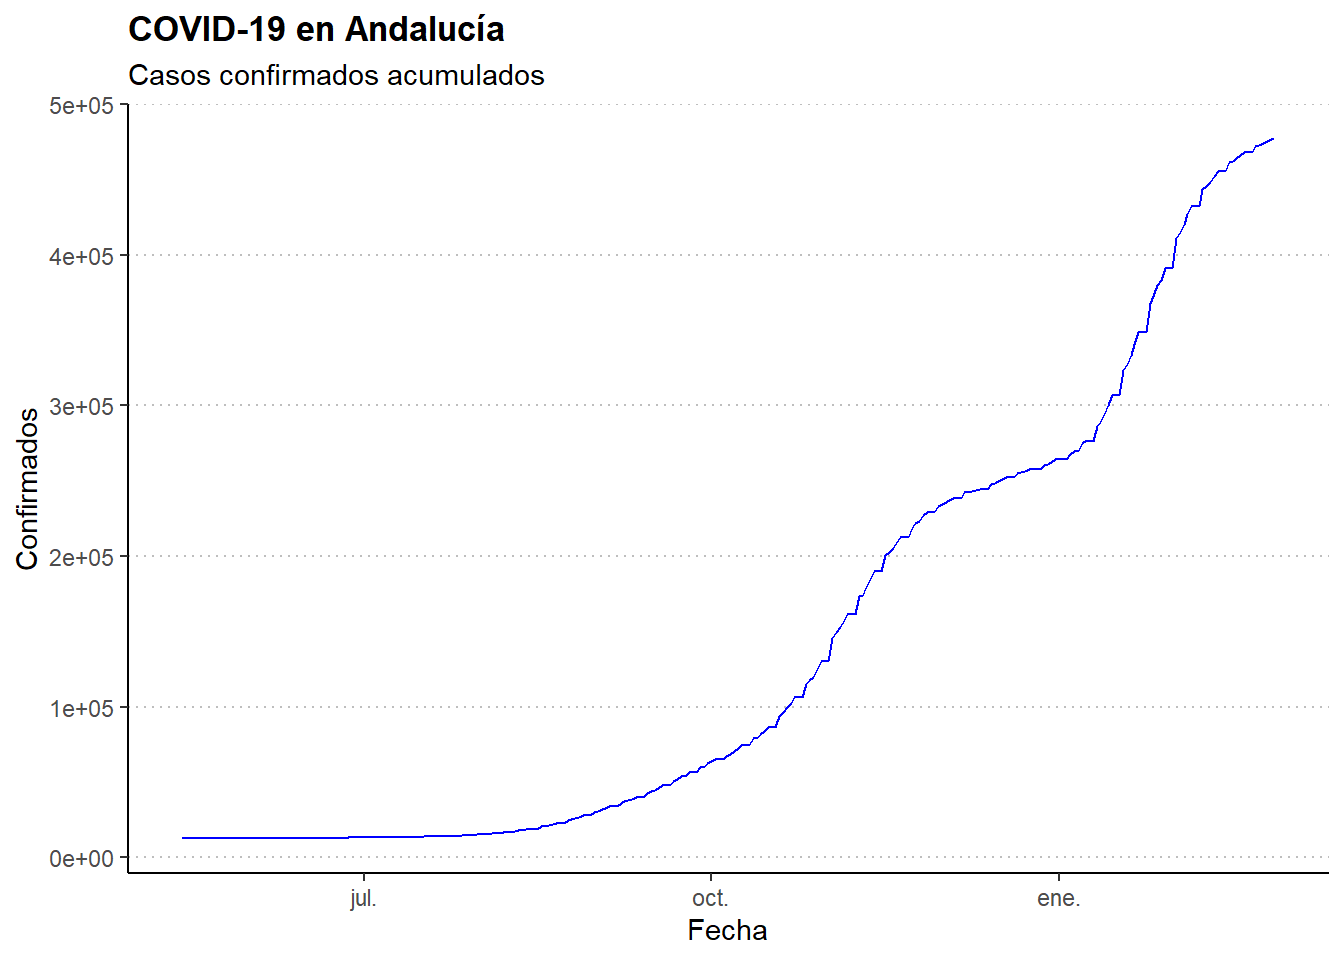
\includegraphics{book_LCC_files/figure-latex/unnamed-chunk-61-1.pdf}

\hypertarget{reglas-de-asociaciuxf3n}{%
\chapter{Reglas de asociación}\label{reglas-de-asociaciuxf3n}}

1.Descargar a local el dataset consumo.csv (en CV).

\begin{Shaded}
\begin{Highlighting}[]
\FunctionTok{library}\NormalTok{(readr)}
\FunctionTok{library}\NormalTok{(tidyverse)}
\FunctionTok{library}\NormalTok{(arules)}
\end{Highlighting}
\end{Shaded}

\begin{verbatim}
## Warning: package 'arules' was built under R version 4.0.5
\end{verbatim}

\begin{verbatim}
## Loading required package: Matrix
\end{verbatim}

\begin{verbatim}
## 
## Attaching package: 'Matrix'
\end{verbatim}

\begin{verbatim}
## The following objects are masked from 'package:tidyr':
## 
##     expand, pack, unpack
\end{verbatim}

\begin{verbatim}
## 
## Attaching package: 'arules'
\end{verbatim}

\begin{verbatim}
## The following object is masked from 'package:dplyr':
## 
##     recode
\end{verbatim}

\begin{verbatim}
## The following objects are masked from 'package:base':
## 
##     abbreviate, write
\end{verbatim}

\begin{Shaded}
\begin{Highlighting}[]
\NormalTok{consumo }\OtherTok{\textless{}{-}} \FunctionTok{read\_csv}\NormalTok{(}\StringTok{"consumo.csv"}\NormalTok{)}
\end{Highlighting}
\end{Shaded}

\begin{verbatim}
## 
## -- Column specification --------------------------------------------------------
## cols(
##   Date = col_date(format = ""),
##   Time = col_time(format = ""),
##   Transaction = col_double(),
##   Item = col_character()
## )
\end{verbatim}

2.Analizar la estructura, tipo,\ldots{} del dataset.

\begin{Shaded}
\begin{Highlighting}[]
\FunctionTok{str}\NormalTok{(consumo)}
\end{Highlighting}
\end{Shaded}

\begin{verbatim}
## spec_tbl_df[,4] [21,293 x 4] (S3: spec_tbl_df/tbl_df/tbl/data.frame)
##  $ Date       : Date[1:21293], format: "2016-10-30" "2016-10-30" ...
##  $ Time       : 'hms' num [1:21293] 09:58:11 10:05:34 10:05:34 10:07:57 ...
##   ..- attr(*, "units")= chr "secs"
##  $ Transaction: num [1:21293] 1 2 2 3 3 3 4 5 5 5 ...
##  $ Item       : chr [1:21293] "Pan" "Salmón" "Salmón" "Chocolate caliente" ...
##  - attr(*, "spec")=
##   .. cols(
##   ..   Date = col_date(format = ""),
##   ..   Time = col_time(format = ""),
##   ..   Transaction = col_double(),
##   ..   Item = col_character()
##   .. )
\end{verbatim}

\begin{Shaded}
\begin{Highlighting}[]
\CommentTok{\# con str vemos que se trata de un spec\_tbl\_df (subclase de data frame) con 21293 filas y 4 columnas (Date,Time,Transaction,Item)}
\end{Highlighting}
\end{Shaded}

\begin{enumerate}
\def\labelenumi{\arabic{enumi}.}
\setcounter{enumi}{2}
\tightlist
\item
  Analizar significado, estructura, tipo,\ldots{} de cada columna.
\end{enumerate}

\begin{Shaded}
\begin{Highlighting}[]
\FunctionTok{str}\NormalTok{(consumo}\SpecialCharTok{$}\NormalTok{Date)}
\end{Highlighting}
\end{Shaded}

\begin{verbatim}
##  Date[1:21293], format: "2016-10-30" "2016-10-30" "2016-10-30" "2016-10-30" "2016-10-30" ...
\end{verbatim}

\begin{Shaded}
\begin{Highlighting}[]
\CommentTok{\# La primera columna corresponde a la fecha (de tipo Date) en la que se ha realizado la compra (transacción)}
\FunctionTok{str}\NormalTok{(consumo}\SpecialCharTok{$}\NormalTok{Time)}
\end{Highlighting}
\end{Shaded}

\begin{verbatim}
##  'hms' num [1:21293] 09:58:11 10:05:34 10:05:34 10:07:57 ...
##  - attr(*, "units")= chr "secs"
\end{verbatim}

\begin{Shaded}
\begin{Highlighting}[]
\CommentTok{\# La segunda columna corresponde a la hora (de tipo num en formato \textquotesingle{}hms\textquotesingle{}(horas,minutos,segundos)) en la que se realizó la compra (transacción)}
\FunctionTok{str}\NormalTok{(consumo}\SpecialCharTok{$}\NormalTok{Transaction)}
\end{Highlighting}
\end{Shaded}

\begin{verbatim}
##  num [1:21293] 1 2 2 3 3 3 4 5 5 5 ...
\end{verbatim}

\begin{Shaded}
\begin{Highlighting}[]
\CommentTok{\# La tercera columna corresponde al número de transacción (de tipo num). Se puede apreciar que en varias filas se repite el número de transacción, esto se debe a que a una misma transacción se le asignan varios Items(4ª columna del data.frame), simulando así un "carrito de la compra"}
\FunctionTok{str}\NormalTok{(consumo}\SpecialCharTok{$}\NormalTok{Item)}
\end{Highlighting}
\end{Shaded}

\begin{verbatim}
##  chr [1:21293] "Pan" "Salmón" "Salmón" "Chocolate caliente" "Jamón" ...
\end{verbatim}

\begin{Shaded}
\begin{Highlighting}[]
\CommentTok{\# En esta cuarta columna se ven representados los items (de tipo char) asociados a las transacciones (compras)}
\end{Highlighting}
\end{Shaded}

\begin{enumerate}
\def\labelenumi{\arabic{enumi}.}
\setcounter{enumi}{3}
\tightlist
\item
  Comandos para ver las primeras filas y las últimas.
\end{enumerate}

\begin{Shaded}
\begin{Highlighting}[]
\CommentTok{\# Comando para ver las primeras filas}
\FunctionTok{head}\NormalTok{(consumo)}
\end{Highlighting}
\end{Shaded}

\begin{verbatim}
## # A tibble: 6 x 4
##   Date       Time     Transaction Item              
##   <date>     <time>         <dbl> <chr>             
## 1 2016-10-30 09:58:11           1 Pan               
## 2 2016-10-30 10:05:34           2 Salmón            
## 3 2016-10-30 10:05:34           2 Salmón            
## 4 2016-10-30 10:07:57           3 Chocolate caliente
## 5 2016-10-30 10:07:57           3 Jamón             
## 6 2016-10-30 10:07:57           3 Galletas
\end{verbatim}

\begin{Shaded}
\begin{Highlighting}[]
\CommentTok{\# Comando para ver las últimas filas}
\FunctionTok{tail}\NormalTok{(consumo)}
\end{Highlighting}
\end{Shaded}

\begin{verbatim}
## # A tibble: 6 x 4
##   Date       Time     Transaction Item        
##   <date>     <time>         <dbl> <chr>       
## 1 2017-04-09 14:32:58        9682 Tacos/Fajita
## 2 2017-04-09 14:32:58        9682 Café        
## 3 2017-04-09 14:32:58        9682 Te          
## 4 2017-04-09 14:57:06        9683 Café        
## 5 2017-04-09 14:57:06        9683 Pastel      
## 6 2017-04-09 15:04:24        9684 Smoothies
\end{verbatim}

\begin{enumerate}
\def\labelenumi{\arabic{enumi}.}
\setcounter{enumi}{4}
\tightlist
\item
  Cambiar los nombres de las columnas: Fecha,Hora, IDcomprador,ProductoComprado.
\end{enumerate}

\begin{Shaded}
\begin{Highlighting}[]
\NormalTok{consumo }\OtherTok{\textless{}{-}}\NormalTok{ consumo }\SpecialCharTok{\%\textgreater{}\%} \FunctionTok{rename}\NormalTok{(}\AttributeTok{Fecha=}\NormalTok{Date, }\AttributeTok{Hora=}\NormalTok{Time, }\AttributeTok{IDcomprador=}\NormalTok{Transaction, }\AttributeTok{ProductoComprado=}\NormalTok{Item)}
\end{Highlighting}
\end{Shaded}

\begin{enumerate}
\def\labelenumi{\arabic{enumi}.}
\setcounter{enumi}{5}
\tightlist
\item
  Hacer un resumen (summary) del dataset y analizar toda la información detalladamente que devuelve el comando.
\end{enumerate}

\begin{Shaded}
\begin{Highlighting}[]
\FunctionTok{summary}\NormalTok{(consumo)}
\end{Highlighting}
\end{Shaded}

\begin{verbatim}
##      Fecha                Hora           IDcomprador   ProductoComprado  
##  Min.   :2016-10-30   Length:21293      Min.   :   1   Length:21293      
##  1st Qu.:2016-12-03   Class1:hms        1st Qu.:2548   Class :character  
##  Median :2017-01-21   Class2:difftime   Median :5067   Mode  :character  
##  Mean   :2017-01-17   Mode  :numeric    Mean   :4952                     
##  3rd Qu.:2017-02-28                     3rd Qu.:7329                     
##  Max.   :2017-04-09                     Max.   :9684
\end{verbatim}

\begin{Shaded}
\begin{Highlighting}[]
\CommentTok{\#En el caso de la columna fecha podemos observar que la máxima (última fecha) es el día 09{-}04{-}2017, o por ejemplo que la menor fecha(primera fecha) en la que se realizó una compra en este data frame fue el día 30{-}10{-}2016}

\CommentTok{\#En el caso de la hora, podemos observar que tenemos 21293 horas en formato hms(horas,minutos,segundos)}

\CommentTok{\#En la columna IDComprador se observa que contiene un rango de valores comprendido entre el 1 y el 9684, siendo la mediana el valor 5067.}

\CommentTok{\#Y por último, en el caso de la columna de ProductoComprado, tenemos 21293 filas con datos de tipo character.}
\end{Highlighting}
\end{Shaded}

7.Implementar una función que usando funciones vectoriales de R (apply, tapply, sapply,\ldots) te devuelva si hay valores NA (mirar valores desconocidos como vienen en el dataset) en las columnas del dataset, si así lo fuera elminarlos del dataset pero guardarlos en un dataset\_auxiliar.

\begin{Shaded}
\begin{Highlighting}[]
\NormalTok{na.in.dataframe }\OtherTok{\textless{}{-}}\ControlFlowTok{function}\NormalTok{(consumo)\{}
\NormalTok{  hay.nas }\OtherTok{\textless{}{-}} \FunctionTok{lapply}\NormalTok{(consumo,}\ControlFlowTok{function}\NormalTok{(x) \{}\StringTok{"NONE"} \SpecialCharTok{\%in\%}\NormalTok{ x\} )  }
\NormalTok{  dataframe.sin.nas }\OtherTok{\textless{}{-}}\NormalTok{ consumo }\SpecialCharTok{\%\textgreater{}\%} \FunctionTok{filter}\NormalTok{(ProductoComprado}\SpecialCharTok{!=}\StringTok{"NONE"}\NormalTok{)}
\NormalTok{  posiciones }\OtherTok{\textless{}{-}} \FunctionTok{which}\NormalTok{(consumo}\SpecialCharTok{$}\NormalTok{ProductoComprado}\SpecialCharTok{==}\StringTok{"NONE"}\NormalTok{)}
  
\FunctionTok{return}\NormalTok{(}\FunctionTok{list}\NormalTok{(hay.nas,dataframe.sin.nas,posiciones))  }
\NormalTok{\}}
\FunctionTok{na.in.dataframe}\NormalTok{(consumo)}
\end{Highlighting}
\end{Shaded}

\begin{verbatim}
## [[1]]
## [[1]]$Fecha
## [1] FALSE
## 
## [[1]]$Hora
## [1] FALSE
## 
## [[1]]$IDcomprador
## [1] FALSE
## 
## [[1]]$ProductoComprado
## [1] TRUE
## 
## 
## [[2]]
## # A tibble: 20,507 x 4
##    Fecha      Hora     IDcomprador ProductoComprado  
##    <date>     <time>         <dbl> <chr>             
##  1 2016-10-30 09:58:11           1 Pan               
##  2 2016-10-30 10:05:34           2 Salmón            
##  3 2016-10-30 10:05:34           2 Salmón            
##  4 2016-10-30 10:07:57           3 Chocolate caliente
##  5 2016-10-30 10:07:57           3 Jamón             
##  6 2016-10-30 10:07:57           3 Galletas          
##  7 2016-10-30 10:08:41           4 Muffin            
##  8 2016-10-30 10:13:03           5 Café              
##  9 2016-10-30 10:13:03           5 Pastel            
## 10 2016-10-30 10:13:03           5 Pan               
## # ... with 20,497 more rows
## 
## [[3]]
##   [1]    27    39    40    67    81    86   127   141   150   168   184   202
##  [13]   227   236   273   283   399   414   420   432   548   561   578   588
##  [25]   629   719   727   789   809   811   817   911   972   981  1010  1011
##  [37]  1106  1130  1146  1203  1225  1261  1265  1289  1383  1395  1399  1446
##  [49]  1453  1461  1684  1744  1903  2191  2333  2353  2374  2379  2421  2442
##  [61]  2544  2551  2574  2598  2601  2610  2619  2634  2638  2643  2676  2713
##  [73]  2729  2757  2900  3000  3004  3013  3015  3080  3134  3140  3143  3156
##  [85]  3199  3270  3285  3289  3292  3295  3306  3308  3310  3318  3456  3492
##  [97]  3527  3536  3558  3573  3577  3713  3722  3732  3733  3741  3851  3862
## [109]  3864  3865  3878  3961  3991  4007  4011  4016  4021  4035  4047  4062
## [121]  4088  4102  4128  4132  4150  4151  4177  4211  4272  4273  4275  4280
## [133]  4287  4288  4291  4298  4300  4301  4304  4305  4314  4325  4356  4383
## [145]  4402  4421  4430  4434  4458  4465  4470  4477  4479  4519  4523  4533
## [157]  4538  4560  4566  4601  4603  4665  4681  4703  4726  4736  4750  4789
## [169]  4798  4834  4835  4837  4842  4847  4849  4853  4916  4919  4928  4938
## [181]  4939  4950  4952  4955  4960  4967  4982  5014  5015  5044  5122  5144
## [193]  5145  5146  5159  5175  5188  5204  5210  5248  5260  5266  5270  5281
## [205]  5288  5289  5402  5424  5431  5432  5445  5446  5461  5487  5526  5531
## [217]  5579  5580  5662  5700  5703  5710  5727  5729  5738  5746  5764  5779
## [229]  5786  5811  5818  5825  5826  5834  5870  5891  5896  5901  5904  5908
## [241]  5936  5975  5982  5992  6001  6005  6040  6041  6059  6075  6082  6098
## [253]  6120  6124  6125  6130  6133  6139  6145  6148  6151  6160  6164  6180
## [265]  6223  6277  6278  6280  6284  6291  6299  6304  6305  6311  6314  6316
## [277]  6322  6323  6330  6395  6398  6462  6473  6524  6555  6566  6572  6577
## [289]  6581  6582  6587  6598  6623  6625  6632  6643  6684  6699  6702  6758
## [301]  6762  6788  6791  6795  6799  6814  6820  6823  6830  6833  6836  6843
## [313]  6853  6856  6865  6923  6969  6983  6993  7002  7012  7014  7059  7095
## [325]  7110  7111  7119  7120  7134  7171  7172  7210  7216  7231  7256  7262
## [337]  7275  7276  7283  7324  7334  7344  7360  7372  7377  7392  7397  7401
## [349]  7410  7414  7478  7484  7485  7496  7499  7513  7515  7526  7529  7546
## [361]  7554  7572  7621  7623  7626  7635  7637  7665  7715  7774  7775  7785
## [373]  7792  7796  7846  7858  7865  7900  7908  7939  7973  7992  7993  8005
## [385]  8006  8007  8030  8050  8051  8058  8059  8114  8125  8132  8137  8139
## [397]  8146  8158  8159  8174  8194  8198  8199  8257  8311  8358  8380  8382
## [409]  8411  8491  8513  8518  8520  8526  8550  8552  8554  8582  8589  8600
## [421]  8603  8620  8624  8625  8641  8672  8680  8691  8695  8700  8704  8706
## [433]  8714  8777  8802  8805  8822  8823  8829  8834  8861  8867  8904  8905
## [445]  8910  8917  8920  8967  8984  8992  8993  9018  9042  9062  9063  9069
## [457]  9091  9100  9151  9155  9166  9182  9207  9248  9252  9286  9297  9298
## [469]  9307  9358  9361  9362  9365  9366  9370  9371  9372  9382  9384  9386
## [481]  9397  9398  9410  9427  9433  9454  9465  9469  9475  9480  9487  9498
## [493]  9499  9500  9507  9509  9512  9566  9569  9575  9582  9634  9638  9648
## [505]  9660  9666  9667  9672  9679  9695  9696  9789  9801  9819  9828  9833
## [517]  9834  9864  9872  9985  9986  9991 10039 10086 10099 10157 10164 10165
## [529] 10176 10177 10214 10361 10436 10442 10551 10599 10625 10633 10637 10650
## [541] 10658 10669 10683 10692 10698 10720 10796 10806 10933 10964 11071 11074
## [553] 11498 11506 11527 11537 11571 11681 11750 11766 11772 11778 11780 11787
## [565] 11794 11820 11830 11870 12016 12039 12093 12155 12200 12340 12395 12408
## [577] 12468 12469 12477 12493 12497 12502 12544 12585 12603 12610 12794 12797
## [589] 12829 13004 13016 13234 13249 13315 13486 13525 13533 13558 13604 13616
## [601] 13751 13778 13785 13818 13828 13842 13961 13996 14044 14181 14234 14272
## [613] 14522 14529 14543 14544 14547 14556 14560 14584 14590 14596 14640 14673
## [625] 14677 14737 14756 14765 14786 14821 14855 14880 14958 14972 15155 15176
## [637] 15371 15397 15495 15498 15545 15571 15587 15596 15600 15610 15686 15727
## [649] 15737 15743 15766 15894 15945 15966 16013 16105 16107 16119 16121 16159
## [661] 16260 16403 16411 16456 16493 16522 16547 16561 16582 16654 16665 16672
## [673] 16682 16713 16746 16769 16787 16799 16802 16835 16842 16845 16908 16940
## [685] 17017 17037 17096 17123 17190 17273 17346 17385 17402 17431 17483 17504
## [697] 17529 17599 17606 17610 17617 17622 17748 17760 17779 17825 17874 18021
## [709] 18038 18064 18080 18122 18209 18247 18254 18270 18275 18289 18316 18317
## [721] 18324 18335 18416 18495 18504 18574 18623 18704 18707 18750 18821 18865
## [733] 18900 18916 19004 19115 19120 19139 19152 19221 19259 19268 19345 19384
## [745] 19437 19538 19588 19751 19856 20010 20012 20025 20105 20130 20188 20191
## [757] 20233 20286 20290 20317 20333 20353 20377 20392 20413 20430 20461 20527
## [769] 20539 20574 20575 20578 20679 20687 20800 20918 20920 20965 21011 21078
## [781] 21081 21109 21123 21255 21256 21267
\end{verbatim}

\begin{Shaded}
\begin{Highlighting}[]
\NormalTok{consumoSinNA }\OtherTok{\textless{}{-}} \FunctionTok{na.in.dataframe}\NormalTok{(consumo)[[}\DecValTok{2}\NormalTok{]]}
\end{Highlighting}
\end{Shaded}

\begin{enumerate}
\def\labelenumi{\arabic{enumi}.}
\setcounter{enumi}{7}
\tightlist
\item
  Calcular número de filas del dataset
\end{enumerate}

\begin{Shaded}
\begin{Highlighting}[]
\NormalTok{nFilas }\OtherTok{\textless{}{-}} \FunctionTok{nrow}\NormalTok{(consumoSinNA)}
\NormalTok{nFilas}
\end{Highlighting}
\end{Shaded}

\begin{verbatim}
## [1] 20507
\end{verbatim}

\begin{enumerate}
\def\labelenumi{\arabic{enumi}.}
\setcounter{enumi}{8}
\tightlist
\item
  Calcula en cuántas fechas distintas se han realizado ventas.
\end{enumerate}

\begin{Shaded}
\begin{Highlighting}[]
\NormalTok{nFechasDistintas }\OtherTok{\textless{}{-}}\NormalTok{ consumoSinNA }\SpecialCharTok{\%\textgreater{}\%} \FunctionTok{group\_by}\NormalTok{(Fecha) }\SpecialCharTok{\%\textgreater{}\%} \FunctionTok{summarise}\NormalTok{(}\AttributeTok{n=}\FunctionTok{n}\NormalTok{())}
\NormalTok{nFechas }\OtherTok{\textless{}{-}} \FunctionTok{length}\NormalTok{(nFechasDistintas}\SpecialCharTok{$}\NormalTok{Fecha)}
\NormalTok{nFechas}
\end{Highlighting}
\end{Shaded}

\begin{verbatim}
## [1] 159
\end{verbatim}

\begin{enumerate}
\def\labelenumi{\arabic{enumi}.}
\setcounter{enumi}{9}
\tightlist
\item
  Calcula cuántos compradores distintos hay en el dataset.
\end{enumerate}

\begin{Shaded}
\begin{Highlighting}[]
\NormalTok{nCompradoresDistintos }\OtherTok{\textless{}{-}}\NormalTok{ consumoSinNA }\SpecialCharTok{\%\textgreater{}\%} \FunctionTok{group\_by}\NormalTok{(IDcomprador) }\SpecialCharTok{\%\textgreater{}\%} \FunctionTok{summarise}\NormalTok{(}\AttributeTok{nComp =} \FunctionTok{n}\NormalTok{())}
\NormalTok{nCompradores }\OtherTok{\textless{}{-}} \FunctionTok{length}\NormalTok{(nCompradoresDistintos}\SpecialCharTok{$}\NormalTok{IDcomprador)}
\NormalTok{nCompradores}
\end{Highlighting}
\end{Shaded}

\begin{verbatim}
## [1] 9465
\end{verbatim}

\begin{enumerate}
\def\labelenumi{\arabic{enumi}.}
\setcounter{enumi}{10}
\tightlist
\item
  Calcula cuántos productos distintos se han vendido. ¿Cuales son los 10 más vendidos? Visualiza con algún gráfico.
\end{enumerate}

\begin{Shaded}
\begin{Highlighting}[]
\NormalTok{nProductosDistintos }\OtherTok{\textless{}{-}}\NormalTok{ consumoSinNA }\SpecialCharTok{\%\textgreater{}\%} \FunctionTok{group\_by}\NormalTok{(ProductoComprado) }\SpecialCharTok{\%\textgreater{}\%} \FunctionTok{summarise}\NormalTok{(}\AttributeTok{nVentas =} \FunctionTok{n}\NormalTok{())}
\NormalTok{nProductos }\OtherTok{\textless{}{-}} \FunctionTok{length}\NormalTok{(nProductosDistintos}\SpecialCharTok{$}\NormalTok{ProductoComprado)}
\NormalTok{nProductos}
\end{Highlighting}
\end{Shaded}

\begin{verbatim}
## [1] 91
\end{verbatim}

\begin{Shaded}
\begin{Highlighting}[]
\NormalTok{nProductosDistintos }\OtherTok{\textless{}{-}}\NormalTok{ nProductosDistintos }\SpecialCharTok{\%\textgreater{}\%} \FunctionTok{arrange}\NormalTok{(}\FunctionTok{desc}\NormalTok{(nVentas))}
\NormalTok{TopTenProductos }\OtherTok{\textless{}{-}}\NormalTok{ nProductosDistintos[}\DecValTok{1}\SpecialCharTok{:}\DecValTok{10}\NormalTok{,]}
\NormalTok{TopTenProductos}
\end{Highlighting}
\end{Shaded}

\begin{verbatim}
## # A tibble: 10 x 2
##    ProductoComprado   nVentas
##    <chr>                <int>
##  1 Café                  5471
##  2 Pan                   3325
##  3 Pastel                1881
##  4 Te                    1435
##  5 Sandwich               771
##  6 Medialuna              616
##  7 Chocolate caliente     590
##  8 Galletas               540
##  9 Brownie                379
## 10 Huevos camperos        374
\end{verbatim}

\begin{Shaded}
\begin{Highlighting}[]
\NormalTok{g1 }\OtherTok{\textless{}{-}}\NormalTok{ TopTenProductos }\SpecialCharTok{\%\textgreater{}\%}
    \FunctionTok{ggplot}\NormalTok{(}\FunctionTok{aes}\NormalTok{(}\AttributeTok{x=}\FunctionTok{reorder}\NormalTok{(ProductoComprado,}\SpecialCharTok{{-}}\NormalTok{nVentas),}\AttributeTok{y=}\NormalTok{nVentas, }\AttributeTok{fill=}\NormalTok{nVentas)) }\SpecialCharTok{+}  \FunctionTok{geom\_bar}\NormalTok{(}\AttributeTok{stat =} \StringTok{"identity"}\NormalTok{) }\SpecialCharTok{+}\FunctionTok{ggtitle}\NormalTok{(}\StringTok{"Top 10 Productos más vendidos"}\NormalTok{)}\SpecialCharTok{+}\FunctionTok{theme}\NormalTok{(}\AttributeTok{plot.title =} \FunctionTok{element\_text}\NormalTok{(}\AttributeTok{face=}\StringTok{"bold"}\NormalTok{))}\SpecialCharTok{+}\FunctionTok{labs}\NormalTok{(}\AttributeTok{x=}\StringTok{"Productos"}\NormalTok{, }\AttributeTok{y =}\StringTok{"Ventas"}\NormalTok{)}\SpecialCharTok{+}\FunctionTok{theme}\NormalTok{(}\AttributeTok{axis.line.x =} \FunctionTok{element\_line}\NormalTok{(}\AttributeTok{color =} \StringTok{"black"}\NormalTok{))}\SpecialCharTok{+}\FunctionTok{theme}\NormalTok{(}\AttributeTok{axis.line.y =} \FunctionTok{element\_line}\NormalTok{(}\AttributeTok{color =} \StringTok{"black"}\NormalTok{))}\SpecialCharTok{+}\FunctionTok{theme}\NormalTok{(}\AttributeTok{panel.grid.major.y =} \FunctionTok{element\_line}\NormalTok{(}\AttributeTok{linetype =} \StringTok{"dotted"}\NormalTok{,}\AttributeTok{colour =} \StringTok{"grey"}\NormalTok{))}\SpecialCharTok{+}\FunctionTok{theme}\NormalTok{(}\AttributeTok{panel.background =} \FunctionTok{element\_rect}\NormalTok{(}\StringTok{"white"}\NormalTok{))}\SpecialCharTok{+}\FunctionTok{theme}\NormalTok{(}\AttributeTok{axis.text.x =} \FunctionTok{element\_text}\NormalTok{(}\AttributeTok{angle =} \DecValTok{14}\NormalTok{))}\SpecialCharTok{+}\FunctionTok{scale\_fill\_gradient}\NormalTok{(}\AttributeTok{low =} \StringTok{"orange"}\NormalTok{,}\AttributeTok{high =} \StringTok{"red"}\NormalTok{)}
\NormalTok{g1}
\end{Highlighting}
\end{Shaded}

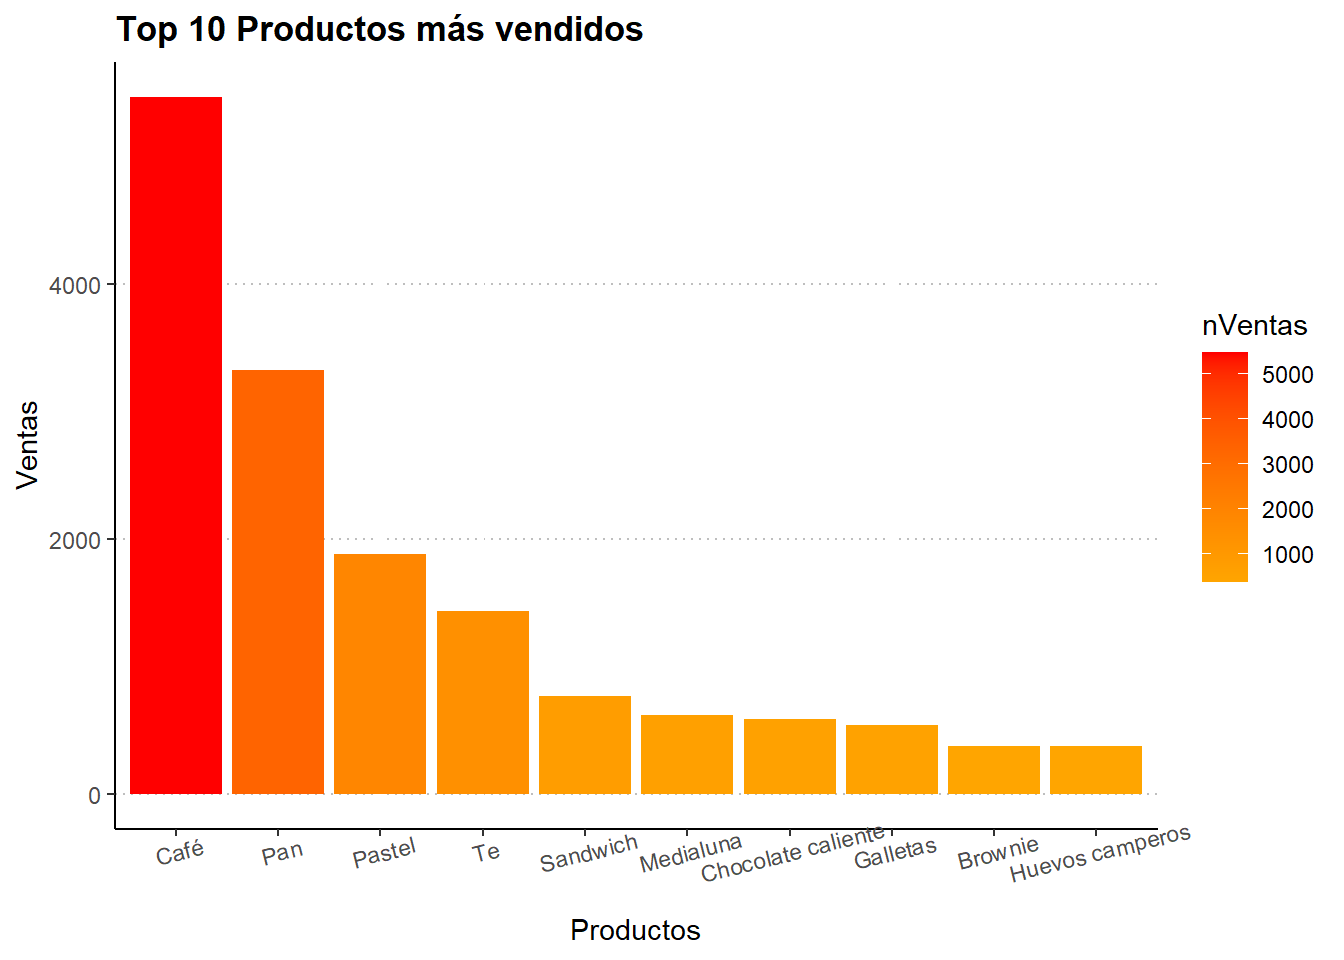
\includegraphics{book_LCC_files/figure-latex/unnamed-chunk-72-1.pdf}
12. Calcula las ventas por franjas y visualiza.

\begin{Shaded}
\begin{Highlighting}[]
\NormalTok{aux }\OtherTok{\textless{}{-}}\NormalTok{ consumoSinNA}
\NormalTok{aux}\SpecialCharTok{$}\NormalTok{Hora }\OtherTok{\textless{}{-}}\NormalTok{ (}\FunctionTok{as.POSIXlt}\NormalTok{(consumoSinNA}\SpecialCharTok{$}\NormalTok{Hora) }\SpecialCharTok{\%\textgreater{}\%} \FunctionTok{format}\NormalTok{(}\StringTok{"\%H"}\NormalTok{))}


\NormalTok{ventasPorFranja }\OtherTok{\textless{}{-}}\NormalTok{  aux }\SpecialCharTok{\%\textgreater{}\%} 
  \FunctionTok{group\_by}\NormalTok{(Hora) }\SpecialCharTok{\%\textgreater{}\%}
  \FunctionTok{summarise}\NormalTok{(}\AttributeTok{n=}\FunctionTok{n}\NormalTok{()) }\SpecialCharTok{\%\textgreater{}\%}
  \FunctionTok{arrange}\NormalTok{(}\FunctionTok{desc}\NormalTok{(Hora))}

\FunctionTok{ggplot}\NormalTok{(ventasPorFranja, }\FunctionTok{aes}\NormalTok{(}\AttributeTok{x=}\NormalTok{Hora, }\AttributeTok{y=}\NormalTok{n)) }\SpecialCharTok{+}
\FunctionTok{geom\_bar}\NormalTok{(}\AttributeTok{stat =} \StringTok{"identity"}\NormalTok{) }\SpecialCharTok{+} \FunctionTok{theme}\NormalTok{(}\AttributeTok{axis.text.x=}\FunctionTok{element\_text}\NormalTok{(}\AttributeTok{angle =} \SpecialCharTok{{-}}\DecValTok{90}\NormalTok{, }\AttributeTok{hjust =} \DecValTok{0}\NormalTok{))}
\end{Highlighting}
\end{Shaded}

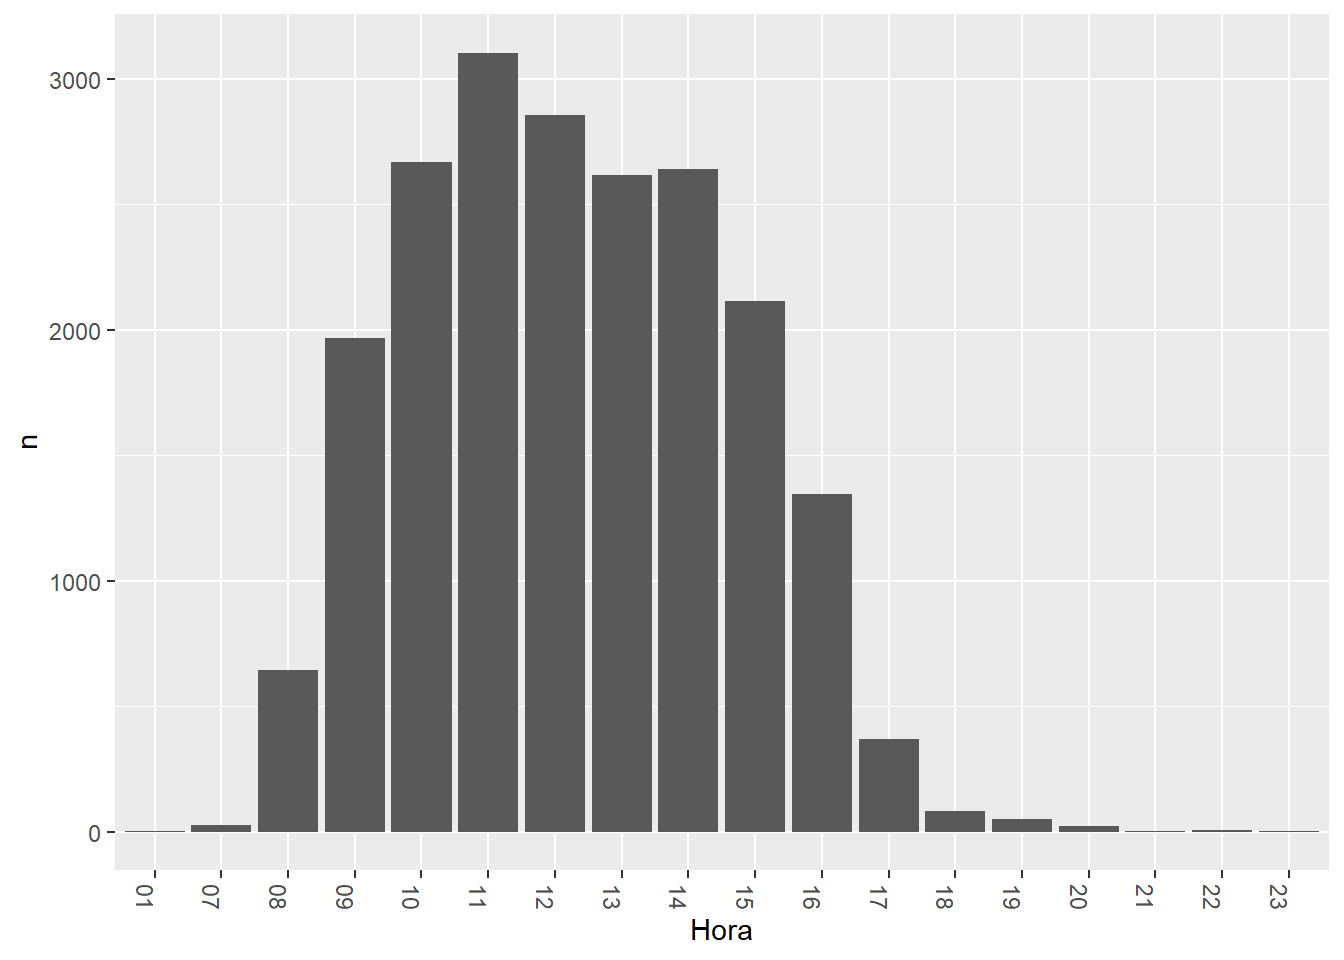
\includegraphics{book_LCC_files/figure-latex/unnamed-chunk-73-1.pdf}

\begin{enumerate}
\def\labelenumi{\arabic{enumi}.}
\setcounter{enumi}{12}
\tightlist
\item
  Separa la fecha en año, mes y día. Obten qué años, meses y días hay más ventas con el objetivo de tener más personal en esas fechas. Visualiza las ventas acumuladas por meses.
\end{enumerate}

\begin{Shaded}
\begin{Highlighting}[]
\NormalTok{aux }\OtherTok{\textless{}{-}}\NormalTok{ consumoSinNA}
\NormalTok{aux }\OtherTok{\textless{}{-}} \FunctionTok{mutate}\NormalTok{(aux,}
\NormalTok{       año }\OtherTok{=}\NormalTok{ aux}\SpecialCharTok{$}\NormalTok{Fecha, }\AttributeTok{mes=}\NormalTok{aux}\SpecialCharTok{$}\NormalTok{Fecha, }\AttributeTok{dia=}\NormalTok{aux}\SpecialCharTok{$}\NormalTok{Fecha)}

\NormalTok{aux}\SpecialCharTok{$}\NormalTok{año }\OtherTok{\textless{}{-}} \FunctionTok{as.numeric}\NormalTok{(}\FunctionTok{format}\NormalTok{(aux}\SpecialCharTok{$}\NormalTok{Fecha,}\StringTok{\textquotesingle{}\%Y\textquotesingle{}}\NormalTok{))}
\NormalTok{aux}\SpecialCharTok{$}\NormalTok{mes }\OtherTok{\textless{}{-}} \FunctionTok{format}\NormalTok{(aux}\SpecialCharTok{$}\NormalTok{Fecha,}\StringTok{\textquotesingle{}\%m\textquotesingle{}}\NormalTok{)}
\NormalTok{aux}\SpecialCharTok{$}\NormalTok{dia }\OtherTok{\textless{}{-}} \FunctionTok{format}\NormalTok{(aux}\SpecialCharTok{$}\NormalTok{Fecha,}\StringTok{\textquotesingle{}\%d\textquotesingle{}}\NormalTok{)}


\NormalTok{ventasPorAño }\OtherTok{\textless{}{-}}\NormalTok{  aux }\SpecialCharTok{\%\textgreater{}\%} 
  \FunctionTok{group\_by}\NormalTok{(año) }\SpecialCharTok{\%\textgreater{}\%}
  \FunctionTok{summarise}\NormalTok{(}\AttributeTok{n=}\FunctionTok{n}\NormalTok{()) }\SpecialCharTok{\%\textgreater{}\%}
  \FunctionTok{arrange}\NormalTok{(}\FunctionTok{desc}\NormalTok{(n))}
\NormalTok{ventasPorAño}
\end{Highlighting}
\end{Shaded}

\begin{verbatim}
## # A tibble: 2 x 2
##     año     n
##   <dbl> <int>
## 1  2017 12363
## 2  2016  8144
\end{verbatim}

\begin{Shaded}
\begin{Highlighting}[]
\NormalTok{ventasPorMes }\OtherTok{\textless{}{-}}\NormalTok{  aux }\SpecialCharTok{\%\textgreater{}\%} 
  \FunctionTok{group\_by}\NormalTok{(mes) }\SpecialCharTok{\%\textgreater{}\%}
  \FunctionTok{summarise}\NormalTok{(}\AttributeTok{n=}\FunctionTok{n}\NormalTok{()) }\SpecialCharTok{\%\textgreater{}\%}
  \FunctionTok{arrange}\NormalTok{(}\FunctionTok{desc}\NormalTok{(n))}
\FunctionTok{head}\NormalTok{(ventasPorMes)}
\end{Highlighting}
\end{Shaded}

\begin{verbatim}
## # A tibble: 6 x 2
##   mes       n
##   <chr> <int>
## 1 11     4436
## 2 03     3944
## 3 02     3906
## 4 01     3356
## 5 12     3339
## 6 04     1157
\end{verbatim}

\begin{Shaded}
\begin{Highlighting}[]
\NormalTok{ventasPorDia }\OtherTok{\textless{}{-}}\NormalTok{  aux }\SpecialCharTok{\%\textgreater{}\%} 
  \FunctionTok{group\_by}\NormalTok{(dia) }\SpecialCharTok{\%\textgreater{}\%}
  \FunctionTok{summarise}\NormalTok{(}\AttributeTok{n=}\FunctionTok{n}\NormalTok{()) }\SpecialCharTok{\%\textgreater{}\%}
  \FunctionTok{arrange}\NormalTok{(}\FunctionTok{desc}\NormalTok{(n))}
\FunctionTok{head}\NormalTok{(ventasPorDia)}
\end{Highlighting}
\end{Shaded}

\begin{verbatim}
## # A tibble: 6 x 2
##   dia       n
##   <chr> <int>
## 1 04     1048
## 2 05      924
## 3 03      858
## 4 19      785
## 5 11      748
## 6 18      745
\end{verbatim}

\begin{Shaded}
\begin{Highlighting}[]
\FunctionTok{ggplot}\NormalTok{(ventasPorMes, }\FunctionTok{aes}\NormalTok{(}\AttributeTok{x=}\NormalTok{mes, }\AttributeTok{y=}\NormalTok{n)) }\SpecialCharTok{+}
\FunctionTok{geom\_bar}\NormalTok{(}\AttributeTok{stat =} \StringTok{"identity"}\NormalTok{) }\SpecialCharTok{+} \FunctionTok{theme}\NormalTok{(}\AttributeTok{axis.text.x=}\FunctionTok{element\_text}\NormalTok{(}\AttributeTok{angle =} \SpecialCharTok{{-}}\DecValTok{90}\NormalTok{, }\AttributeTok{hjust =} \DecValTok{0}\NormalTok{))}
\end{Highlighting}
\end{Shaded}

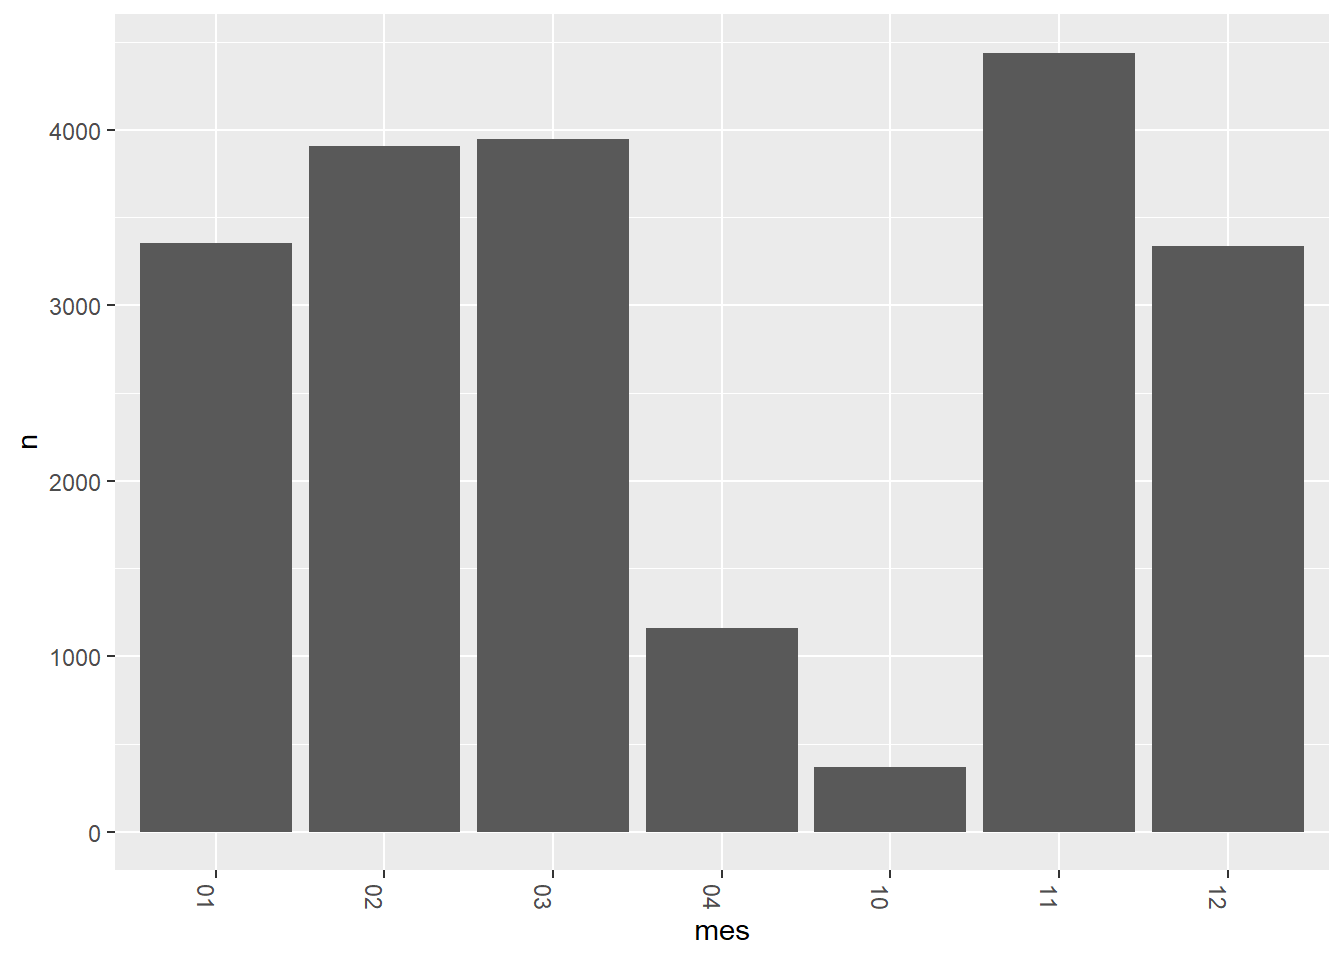
\includegraphics{book_LCC_files/figure-latex/unnamed-chunk-74-1.pdf}

\begin{enumerate}
\def\labelenumi{\arabic{enumi}.}
\setcounter{enumi}{13}
\tightlist
\item
  Usa split para construir a partir de dataset una lista con nombre lista.compra.usuarios en la que cada elemento de la lista es cada comprador junto con todos los productos que ha comprado
\end{enumerate}

\begin{Shaded}
\begin{Highlighting}[]
\NormalTok{consumoSinNASoloProductos }\OtherTok{\textless{}{-}}\NormalTok{ consumoSinNA }\SpecialCharTok{\%\textgreater{}\%} \FunctionTok{select}\NormalTok{(IDcomprador,ProductoComprado)}
\NormalTok{lista.compra.usuarios }\OtherTok{\textless{}{-}} \FunctionTok{split}\NormalTok{(consumoSinNA [,}\StringTok{"ProductoComprado"}\NormalTok{],}\AttributeTok{f=}\NormalTok{consumoSinNA}\SpecialCharTok{$}\NormalTok{IDcomprador)}
\NormalTok{lista.compra.usuarios }\OtherTok{\textless{}{-}}\FunctionTok{lapply}\NormalTok{(lista.compra.usuarios,}\ControlFlowTok{function}\NormalTok{(x)\{}\FunctionTok{as.list}\NormalTok{(x}\SpecialCharTok{$}\NormalTok{ProductoComprado)\})}
\NormalTok{lista.compra.usuarios[}\DecValTok{1}\SpecialCharTok{:}\DecValTok{3}\NormalTok{]}
\end{Highlighting}
\end{Shaded}

\begin{verbatim}
## $`1`
## $`1`[[1]]
## [1] "Pan"
## 
## 
## $`2`
## $`2`[[1]]
## [1] "Salmón"
## 
## $`2`[[2]]
## [1] "Salmón"
## 
## 
## $`3`
## $`3`[[1]]
## [1] "Chocolate caliente"
## 
## $`3`[[2]]
## [1] "Jamón"
## 
## $`3`[[3]]
## [1] "Galletas"
\end{verbatim}

\begin{enumerate}
\def\labelenumi{\arabic{enumi}.}
\setcounter{enumi}{14}
\tightlist
\item
  Hacer summary de lista.compra.usuarios
\end{enumerate}

\begin{Shaded}
\begin{Highlighting}[]
\CommentTok{\#He hecho el summary de los 20 primeros porque si lo hiciera de la lista entera aparecerían unas 9000 filas}
\FunctionTok{summary}\NormalTok{(lista.compra.usuarios[}\DecValTok{1}\SpecialCharTok{:}\DecValTok{20}\NormalTok{])}
\end{Highlighting}
\end{Shaded}

\begin{verbatim}
##    Length Class  Mode
## 1  1      -none- list
## 2  2      -none- list
## 3  3      -none- list
## 4  1      -none- list
## 5  3      -none- list
## 6  3      -none- list
## 7  4      -none- list
## 8  2      -none- list
## 9  2      -none- list
## 10 2      -none- list
## 11 3      -none- list
## 12 5      -none- list
## 13 3      -none- list
## 14 3      -none- list
## 15 2      -none- list
## 16 3      -none- list
## 17 1      -none- list
## 18 1      -none- list
## 19 2      -none- list
## 20 2      -none- list
\end{verbatim}

\begin{enumerate}
\def\labelenumi{\arabic{enumi}.}
\setcounter{enumi}{15}
\tightlist
\item
  Contar cuántos usuarios hay en la lista lista.compra.usuarios
\end{enumerate}

\begin{Shaded}
\begin{Highlighting}[]
\FunctionTok{length}\NormalTok{(lista.compra.usuarios)}
\end{Highlighting}
\end{Shaded}

\begin{verbatim}
## [1] 9465
\end{verbatim}

\begin{enumerate}
\def\labelenumi{\arabic{enumi}.}
\setcounter{enumi}{16}
\tightlist
\item
  Convertir a tipo de datos transacciones. Guardar en Tlista.compra.usuarios.
\end{enumerate}

\begin{Shaded}
\begin{Highlighting}[]
\CommentTok{\#Al intentar convertir la lista a transacciones aparecía el error: Error in asMethod(object) : can coerce list with atomic components only; por eso los apartados que aparecen a continuación están comentados, pero con las instrucciones con las que se llevarían a cabo.}
\CommentTok{\#Tlista.compra.usuarios \textless{}{-} as(lista.compra.usuarios,"transactions")}
\end{Highlighting}
\end{Shaded}

\begin{enumerate}
\def\labelenumi{\arabic{enumi}.}
\setcounter{enumi}{17}
\tightlist
\item
  Hacer inspect de los dos primeros valores de Tlista.compra.usuarios.
\end{enumerate}

\begin{Shaded}
\begin{Highlighting}[]
\CommentTok{\#inspect(Tlista.compra.usuarios[1:2])}
\end{Highlighting}
\end{Shaded}

\begin{enumerate}
\def\labelenumi{\arabic{enumi}.}
\setcounter{enumi}{18}
\tightlist
\item
  Buscar ayuda de itemFrequencyPlot para visualizar las 10 transacciones más frecuentes.
\end{enumerate}

\begin{Shaded}
\begin{Highlighting}[]
\CommentTok{\#itemFrequencyPlot(Tlista.compra.usuarios, topN = 10, col = rainbow(4))}
\end{Highlighting}
\end{Shaded}

\begin{enumerate}
\def\labelenumi{\arabic{enumi}.}
\setcounter{enumi}{19}
\tightlist
\item
  Generar las reglas de asociación con 80\% de confianza y 15\% de soporte. (varias estos úmbrales si no son adecuadas las reglas que obtienes - demasiadas y no acaba o pocas)
\end{enumerate}

\begin{Shaded}
\begin{Highlighting}[]
\CommentTok{\#mis\_reglas \textless{}{-} apriori(Tlista.compra.usuarios,parameter = list(supp=0.15, conf=0.80, minlen=2))}
\end{Highlighting}
\end{Shaded}

\begin{enumerate}
\def\labelenumi{\arabic{enumi}.}
\setcounter{enumi}{20}
\tightlist
\item
  Ver las reglas generadas y ordenalas por lift. Guarda el resultado en una variable nueva.
\end{enumerate}

\begin{Shaded}
\begin{Highlighting}[]
\CommentTok{\#inspect(mis\_reglas[1:10]) \#vemos la reglas generadas}
\CommentTok{\#mis\_reglas\_ordenadas \textless{}{-} sort(mis\_reglas,by="lift",decreasing = TRUE) \#ordenamos las reglas por lift}
\CommentTok{\#inspect(mis\_reglas\_ordenadas[1:10]) \#vemos las reglas ordenadas por lift}
\end{Highlighting}
\end{Shaded}

\begin{enumerate}
\def\labelenumi{\arabic{enumi}.}
\setcounter{enumi}{21}
\tightlist
\item
  Elimina todas las reglas redundantes.
\end{enumerate}

\begin{Shaded}
\begin{Highlighting}[]
\CommentTok{\#reglas\_no\_redundantes \textless{}{-} mis\_reglas\_ordenadas[!is.redundant(x = mis\_reglas\_ordenadas, measure = "confidence")]}
\end{Highlighting}
\end{Shaded}

\hypertarget{fca}{%
\chapter{FCA}\label{fca}}

\hypertarget{tutorial-ganter-conceptos}{%
\section{Tutorial Ganter (Conceptos)}\label{tutorial-ganter-conceptos}}

\begin{Shaded}
\begin{Highlighting}[]
\FunctionTok{library}\NormalTok{(}\StringTok{\textquotesingle{}fcaR\textquotesingle{}}\NormalTok{)}
\end{Highlighting}
\end{Shaded}

\begin{verbatim}
## 
## Attaching package: 'fcaR'
\end{verbatim}

\begin{verbatim}
## The following object is masked from 'package:purrr':
## 
##     as_vector
\end{verbatim}

\begin{Shaded}
\begin{Highlighting}[]
\FunctionTok{library}\NormalTok{(readr)}
\FunctionTok{library}\NormalTok{(tidyverse)}

\NormalTok{dataset\_ganter }\OtherTok{\textless{}{-}} \FunctionTok{read.csv}\NormalTok{(}\StringTok{"contextformal\_tutorialGanter.csv"}\NormalTok{, }\AttributeTok{sep=}\StringTok{";"}\NormalTok{)}
\FunctionTok{View}\NormalTok{(dataset\_ganter)}
\FunctionTok{rownames}\NormalTok{(dataset\_ganter) }\OtherTok{\textless{}{-}}\NormalTok{ dataset\_ganter[[}\DecValTok{1}\NormalTok{]]}

\NormalTok{dataset\_ganter[[}\DecValTok{1}\NormalTok{]] }\OtherTok{\textless{}{-}} \ConstantTok{NULL}
\end{Highlighting}
\end{Shaded}

Introduce el dataset anterior en un contexto formal de nombre fc\_ganter usando el paquete fcaR Imprime el contexto formal (print). Haz plot también del contexto formal.

\begin{Shaded}
\begin{Highlighting}[]
\NormalTok{fc\_ganter }\OtherTok{\textless{}{-}}\NormalTok{ FormalContext}\SpecialCharTok{$}\FunctionTok{new}\NormalTok{(dataset\_ganter)}
\FunctionTok{print}\NormalTok{(fc\_ganter)}
\end{Highlighting}
\end{Shaded}

\begin{verbatim}
## FormalContext with 7 objects and 9 attributes.
##               needs.water   lives.in.water   lives.on.hand   needs.chlorophyll  
##        Leech       X              X                                             
##        Bream       X              X                                             
##         Frog       X              X                X                            
##   Spike-Weed       X              X                                  X          
##         Reed       X              X                X                 X          
##         Bean       X                               X                 X          
##        Maize       X                               X                 X          
## Other attributes are: two.seeds.leaves, one.seed.leaf, can.move.around,
## has.limbs, suckles.its.offspring
\end{verbatim}

\begin{Shaded}
\begin{Highlighting}[]
\FunctionTok{plot}\NormalTok{(fc\_ganter)}
\end{Highlighting}
\end{Shaded}

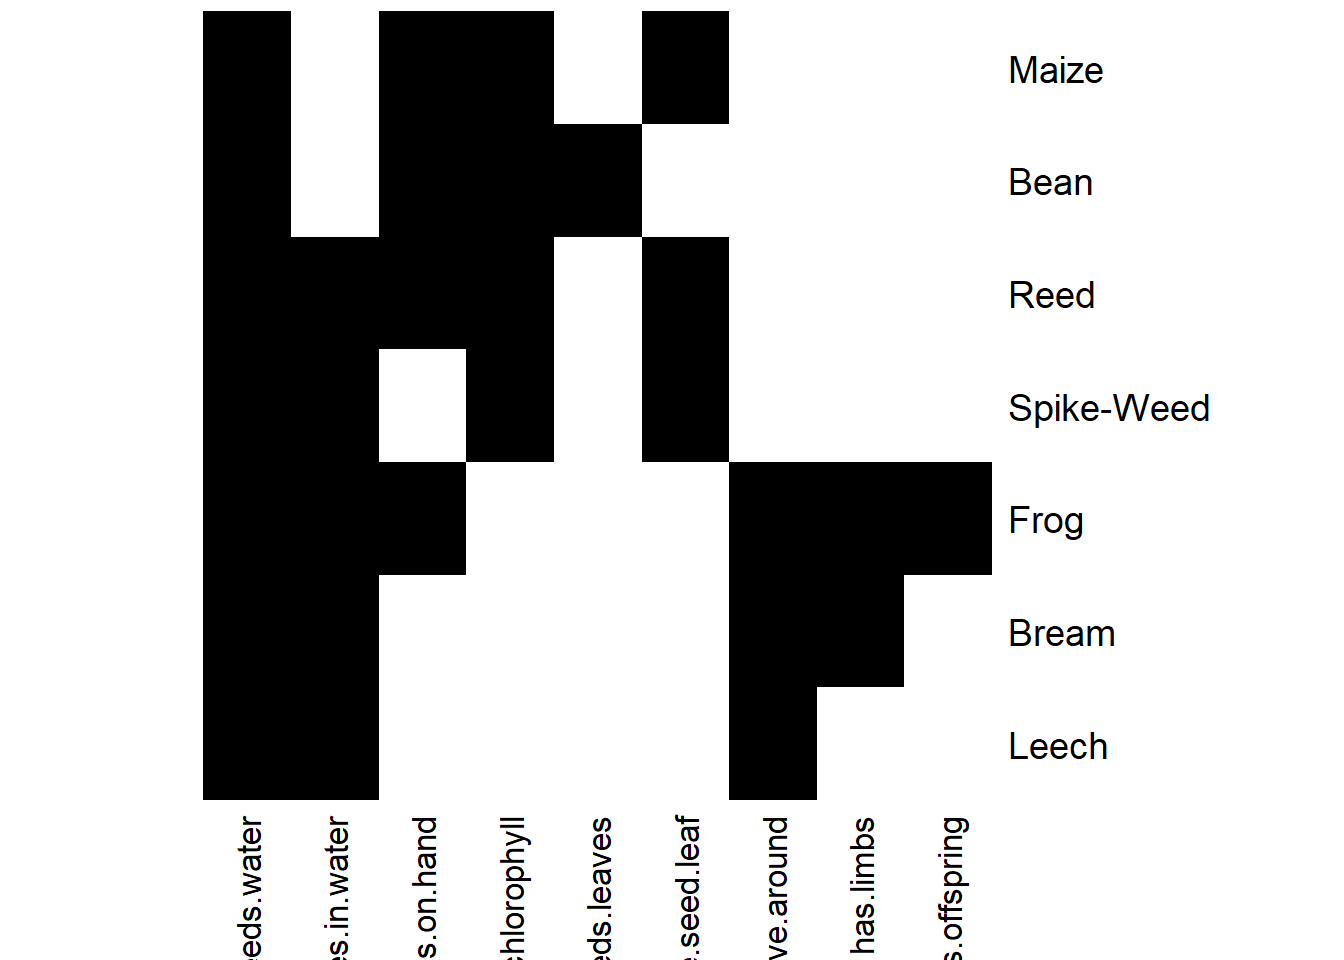
\includegraphics{book_LCC_files/figure-latex/unnamed-chunk-85-1.pdf}
Convierte a latex el contexto formal. En el Rmd introduce el código latex del contexto formal para visualizarlo.

\begin{Shaded}
\begin{Highlighting}[]
\NormalTok{fc\_ganter}\SpecialCharTok{$}\FunctionTok{to\_latex}\NormalTok{()}
\end{Highlighting}
\end{Shaded}

\begin{verbatim}
## \begin{table} \centering \begin{tabular}{lccccccccc}
## \toprule
##  & needs.water & lives.in.water & lives.on.hand & needs.chlorophyll & two.seeds.leaves & one.seed.leaf & can.move.around & has.limbs & suckles.its.offspring\\
## \midrule
## Leech & $\times$ & $\times$ &   &   &   &   & $\times$ &   &  \\ 
## Bream & $\times$ & $\times$ &   &   &   &   & $\times$ & $\times$ &  \\ 
## Frog & $\times$ & $\times$ & $\times$ &   &   &   & $\times$ & $\times$ & $\times$\\ 
## Spike-Weed & $\times$ & $\times$ &   & $\times$ &   & $\times$ &   &   &  \\ 
## Reed & $\times$ & $\times$ & $\times$ & $\times$ &   & $\times$ &   &   &  \\ 
## Bean & $\times$ &   & $\times$ & $\times$ & $\times$ &   &   &   &  \\ 
## Maize & $\times$ &   & $\times$ & $\times$ &   & $\times$ &   &   &  \\
## \bottomrule
## \end{tabular} \caption{\label{}} \end{table}
\end{verbatim}

Guarda todos los atributos en una variable attr\_ganter usando los comandos del paquete fcaR

\begin{Shaded}
\begin{Highlighting}[]
\NormalTok{attr\_ganter }\OtherTok{\textless{}{-}}\NormalTok{ fc\_ganter}\SpecialCharTok{$}\NormalTok{attributes}
\NormalTok{attr\_ganter}
\end{Highlighting}
\end{Shaded}

\begin{verbatim}
## [1] "needs.water"           "lives.in.water"        "lives.on.hand"        
## [4] "needs.chlorophyll"     "two.seeds.leaves"      "one.seed.leaf"        
## [7] "can.move.around"       "has.limbs"             "suckles.its.offspring"
\end{verbatim}

Guarda todos los objetos en una variable obj\_ganter usando los comandos del paquete fcaR.

\begin{Shaded}
\begin{Highlighting}[]
\NormalTok{obj\_ganter }\OtherTok{\textless{}{-}}\NormalTok{ fc\_ganter}\SpecialCharTok{$}\NormalTok{objects}
\NormalTok{obj\_ganter}
\end{Highlighting}
\end{Shaded}

\begin{verbatim}
## [1] "Leech"      "Bream"      "Frog"       "Spike-Weed" "Reed"      
## [6] "Bean"       "Maize"
\end{verbatim}

¿De que tipo es la variable attr\_ganter?

\begin{Shaded}
\begin{Highlighting}[]
\FunctionTok{class}\NormalTok{(attr\_ganter)}
\end{Highlighting}
\end{Shaded}

\begin{verbatim}
## [1] "character"
\end{verbatim}

\begin{Shaded}
\begin{Highlighting}[]
\FunctionTok{str}\NormalTok{(attr\_ganter)}
\end{Highlighting}
\end{Shaded}

\begin{verbatim}
##  chr [1:9] "needs.water" "lives.in.water" "lives.on.hand" ...
\end{verbatim}

¿De que tipo es la variable attr\_objetos?

\begin{Shaded}
\begin{Highlighting}[]
\FunctionTok{class}\NormalTok{(obj\_ganter)}
\end{Highlighting}
\end{Shaded}

\begin{verbatim}
## [1] "character"
\end{verbatim}

\begin{Shaded}
\begin{Highlighting}[]
\FunctionTok{str}\NormalTok{(obj\_ganter)}
\end{Highlighting}
\end{Shaded}

\begin{verbatim}
##  chr [1:7] "Leech" "Bream" "Frog" "Spike-Weed" "Reed" "Bean" "Maize"
\end{verbatim}

Visualizando el contexto formal y utilizando los operadores de derivación, calcula dos conceptos sin usar el método que calcula todos los conceptos.

\begin{Shaded}
\begin{Highlighting}[]
\NormalTok{S1 }\OtherTok{\textless{}{-}}\NormalTok{ SparseSet}\SpecialCharTok{$}\FunctionTok{new}\NormalTok{(}\AttributeTok{attributes =}\NormalTok{ fc\_ganter}\SpecialCharTok{$}\NormalTok{objects)}
\NormalTok{S1}\SpecialCharTok{$}\FunctionTok{assign}\NormalTok{(}\AttributeTok{Leech =} \DecValTok{1}\NormalTok{, }\AttributeTok{Bream =} \DecValTok{1}\NormalTok{)}
\NormalTok{S1}
\end{Highlighting}
\end{Shaded}

\begin{verbatim}
## {Leech, Bream}
\end{verbatim}

\begin{Shaded}
\begin{Highlighting}[]
\NormalTok{fc\_ganter}\SpecialCharTok{$}\FunctionTok{intent}\NormalTok{(S1)}
\end{Highlighting}
\end{Shaded}

\begin{verbatim}
## {needs.water, lives.in.water, can.move.around}
\end{verbatim}

\begin{Shaded}
\begin{Highlighting}[]
\NormalTok{S2 }\OtherTok{\textless{}{-}}\NormalTok{ SparseSet}\SpecialCharTok{$}\FunctionTok{new}\NormalTok{(}\AttributeTok{attributes =}\NormalTok{ fc\_ganter}\SpecialCharTok{$}\NormalTok{attributes)}
\NormalTok{S2}\SpecialCharTok{$}\FunctionTok{assign}\NormalTok{(}\AttributeTok{needs.water =} \DecValTok{1}\NormalTok{, }\AttributeTok{lives.in.water =} \DecValTok{1}\NormalTok{, }\AttributeTok{can.move.around =} \DecValTok{1}\NormalTok{)}
\NormalTok{S2}
\end{Highlighting}
\end{Shaded}

\begin{verbatim}
## {needs.water, lives.in.water, can.move.around}
\end{verbatim}

\begin{Shaded}
\begin{Highlighting}[]
\NormalTok{fc\_ganter}\SpecialCharTok{$}\FunctionTok{extent}\NormalTok{(S2)}
\end{Highlighting}
\end{Shaded}

\begin{verbatim}
## {Leech, Bream, Frog}
\end{verbatim}

Usar método de fcaR para calcular todos los conceptos.

\begin{Shaded}
\begin{Highlighting}[]
\NormalTok{fc\_ganter}\SpecialCharTok{$}\FunctionTok{find\_concepts}\NormalTok{()}
\NormalTok{fc\_ganter}\SpecialCharTok{$}\NormalTok{concepts}
\end{Highlighting}
\end{Shaded}

\begin{verbatim}
## A set of 15 concepts:
## 1: ({Leech, Bream, Frog, Spike-Weed, Reed, Bean, Maize}, {needs.water})
## 2: ({Spike-Weed, Reed, Bean, Maize}, {needs.water, needs.chlorophyll})
## 3: ({Spike-Weed, Reed, Maize}, {needs.water, needs.chlorophyll, one.seed.leaf})
## 4: ({Frog, Reed, Bean, Maize}, {needs.water, lives.on.hand})
## 5: ({Reed, Bean, Maize}, {needs.water, lives.on.hand, needs.chlorophyll})
## 6: ({Reed, Maize}, {needs.water, lives.on.hand, needs.chlorophyll, one.seed.leaf})
## 7: ({Bean}, {needs.water, lives.on.hand, needs.chlorophyll, two.seeds.leaves})
## 8: ({Leech, Bream, Frog, Spike-Weed, Reed}, {needs.water, lives.in.water})
## 9: ({Leech, Bream, Frog}, {needs.water, lives.in.water, can.move.around})
## 10: ({Bream, Frog}, {needs.water, lives.in.water, can.move.around, has.limbs})
## 11: ({Spike-Weed, Reed}, {needs.water, lives.in.water, needs.chlorophyll, one.seed.leaf})
## 12: ({Frog, Reed}, {needs.water, lives.in.water, lives.on.hand})
## 13: ({Frog}, {needs.water, lives.in.water, lives.on.hand, can.move.around, has.limbs, suckles.its.offspring})
## 14: ({Reed}, {needs.water, lives.in.water, lives.on.hand, needs.chlorophyll, one.seed.leaf})
## 15: ({}, {needs.water, lives.in.water, lives.on.hand, needs.chlorophyll, two.seeds.leaves, one.seed.leaf, can.move.around, has.limbs, suckles.its.offspring})
\end{verbatim}

¿Cuantos conceptos hemos calculado a partir del contexto formal?

\begin{Shaded}
\begin{Highlighting}[]
\NormalTok{fc\_ganter}\SpecialCharTok{$}\NormalTok{concepts}\SpecialCharTok{$}\FunctionTok{size}\NormalTok{()}
\end{Highlighting}
\end{Shaded}

\begin{verbatim}
## [1] 15
\end{verbatim}

Muestra los 10 primeros conceptos.

\begin{Shaded}
\begin{Highlighting}[]
\NormalTok{fc\_ganter}\SpecialCharTok{$}\NormalTok{concepts[}\DecValTok{1}\SpecialCharTok{:}\DecValTok{10}\NormalTok{]}
\end{Highlighting}
\end{Shaded}

\begin{verbatim}
## ({Leech, Bream, Frog, Spike-Weed, Reed, Bean, Maize}, {needs.water})
## ({Spike-Weed, Reed, Bean, Maize}, {needs.water, needs.chlorophyll})
## ({Spike-Weed, Reed, Maize}, {needs.water, needs.chlorophyll, one.seed.leaf})
## ({Frog, Reed, Bean, Maize}, {needs.water, lives.on.hand})
## ({Reed, Bean, Maize}, {needs.water, lives.on.hand, needs.chlorophyll})
## ({Reed, Maize}, {needs.water, lives.on.hand, needs.chlorophyll, one.seed.leaf})
## ({Bean}, {needs.water, lives.on.hand, needs.chlorophyll, two.seeds.leaves})
## ({Leech, Bream, Frog, Spike-Weed, Reed}, {needs.water, lives.in.water})
## ({Leech, Bream, Frog}, {needs.water, lives.in.water, can.move.around})
## ({Bream, Frog}, {needs.water, lives.in.water, can.move.around, has.limbs})
\end{verbatim}

Dibuja el retículo de conceptos

\begin{Shaded}
\begin{Highlighting}[]
\NormalTok{fc\_ganter}\SpecialCharTok{$}\NormalTok{concepts}\SpecialCharTok{$}\FunctionTok{plot}\NormalTok{()}
\end{Highlighting}
\end{Shaded}

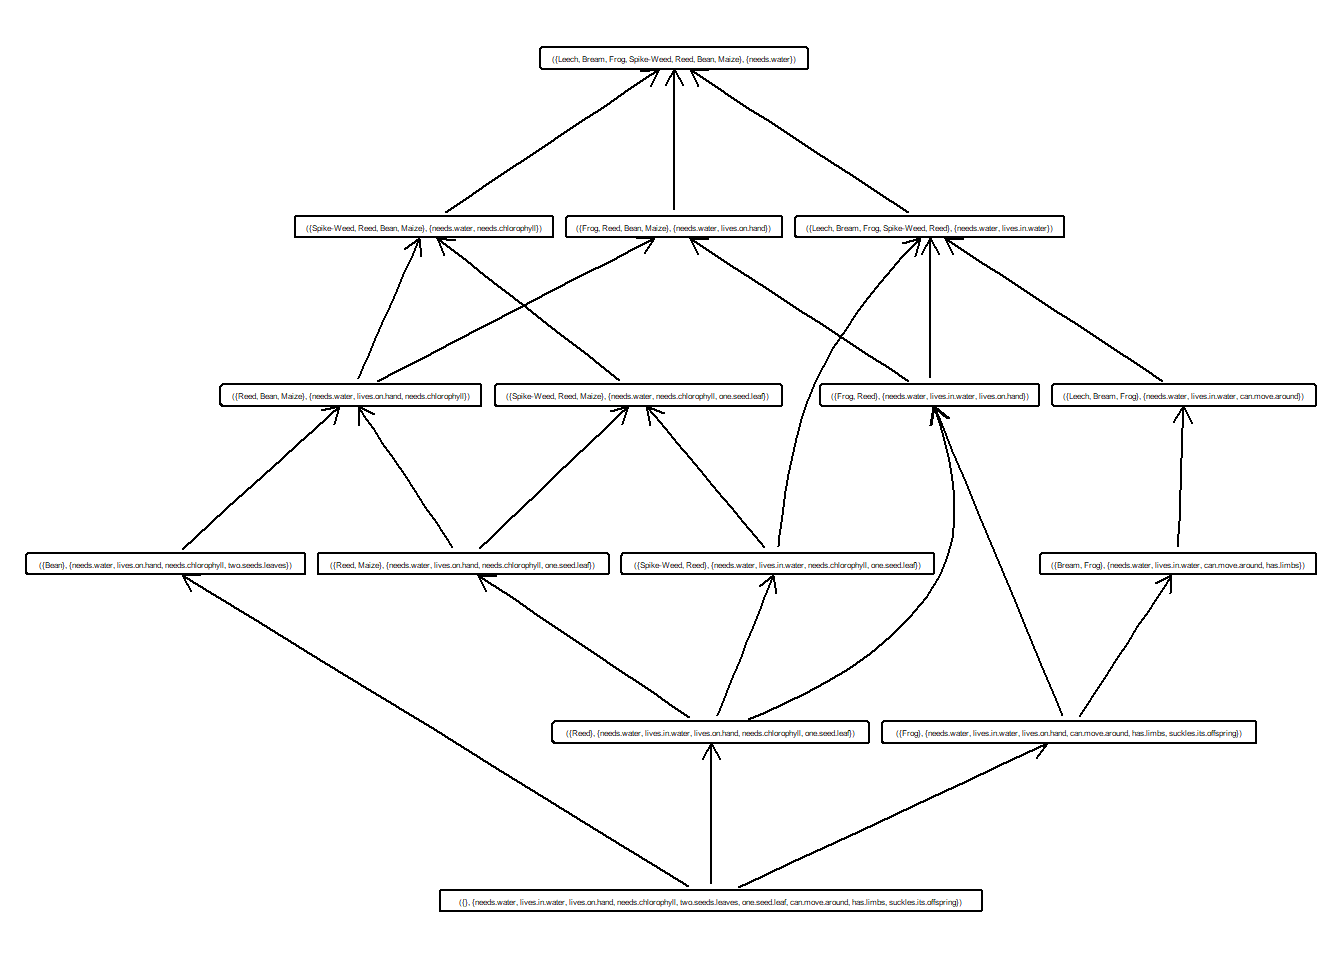
\includegraphics{book_LCC_files/figure-latex/unnamed-chunk-95-1.pdf}
Calcular y guardar en una variable el subretículo con soporte mayor que 0.3.

\begin{Shaded}
\begin{Highlighting}[]
\NormalTok{idx }\OtherTok{\textless{}{-}} \FunctionTok{which}\NormalTok{(fc\_ganter}\SpecialCharTok{$}\NormalTok{concepts}\SpecialCharTok{$}\FunctionTok{support}\NormalTok{() }\SpecialCharTok{\textgreater{}} \FloatTok{0.3}\NormalTok{)}
\NormalTok{sublattice }\OtherTok{\textless{}{-}}\NormalTok{ fc\_ganter}\SpecialCharTok{$}\NormalTok{concepts}\SpecialCharTok{$}\FunctionTok{sublattice}\NormalTok{(idx)}
\NormalTok{sublattice}
\end{Highlighting}
\end{Shaded}

\begin{verbatim}
## A set of 13 concepts:
## 1: ({Leech, Bream, Frog, Spike-Weed, Reed, Bean, Maize}, {needs.water})
## 2: ({Spike-Weed, Reed, Bean, Maize}, {needs.water, needs.chlorophyll})
## 3: ({Spike-Weed, Reed, Maize}, {needs.water, needs.chlorophyll, one.seed.leaf})
## 4: ({Frog, Reed, Bean, Maize}, {needs.water, lives.on.hand})
## 5: ({Reed, Bean, Maize}, {needs.water, lives.on.hand, needs.chlorophyll})
## 6: ({Reed, Maize}, {needs.water, lives.on.hand, needs.chlorophyll, one.seed.leaf})
## 7: ({Leech, Bream, Frog, Spike-Weed, Reed}, {needs.water, lives.in.water})
## 8: ({Leech, Bream, Frog}, {needs.water, lives.in.water, can.move.around})
## 9: ({Spike-Weed, Reed}, {needs.water, lives.in.water, needs.chlorophyll, one.seed.leaf})
## 10: ({Frog, Reed}, {needs.water, lives.in.water, lives.on.hand})
## 11: ({Frog}, {needs.water, lives.in.water, lives.on.hand, can.move.around, has.limbs, suckles.its.offspring})
## 12: ({Reed}, {needs.water, lives.in.water, lives.on.hand, needs.chlorophyll, one.seed.leaf})
## 13: ({}, {needs.water, lives.in.water, lives.on.hand, needs.chlorophyll, two.seeds.leaves, one.seed.leaf, can.move.around, has.limbs, suckles.its.offspring})
\end{verbatim}

Dibujar dicho subretículo.

\begin{Shaded}
\begin{Highlighting}[]
\FunctionTok{plot}\NormalTok{(sublattice)}
\end{Highlighting}
\end{Shaded}

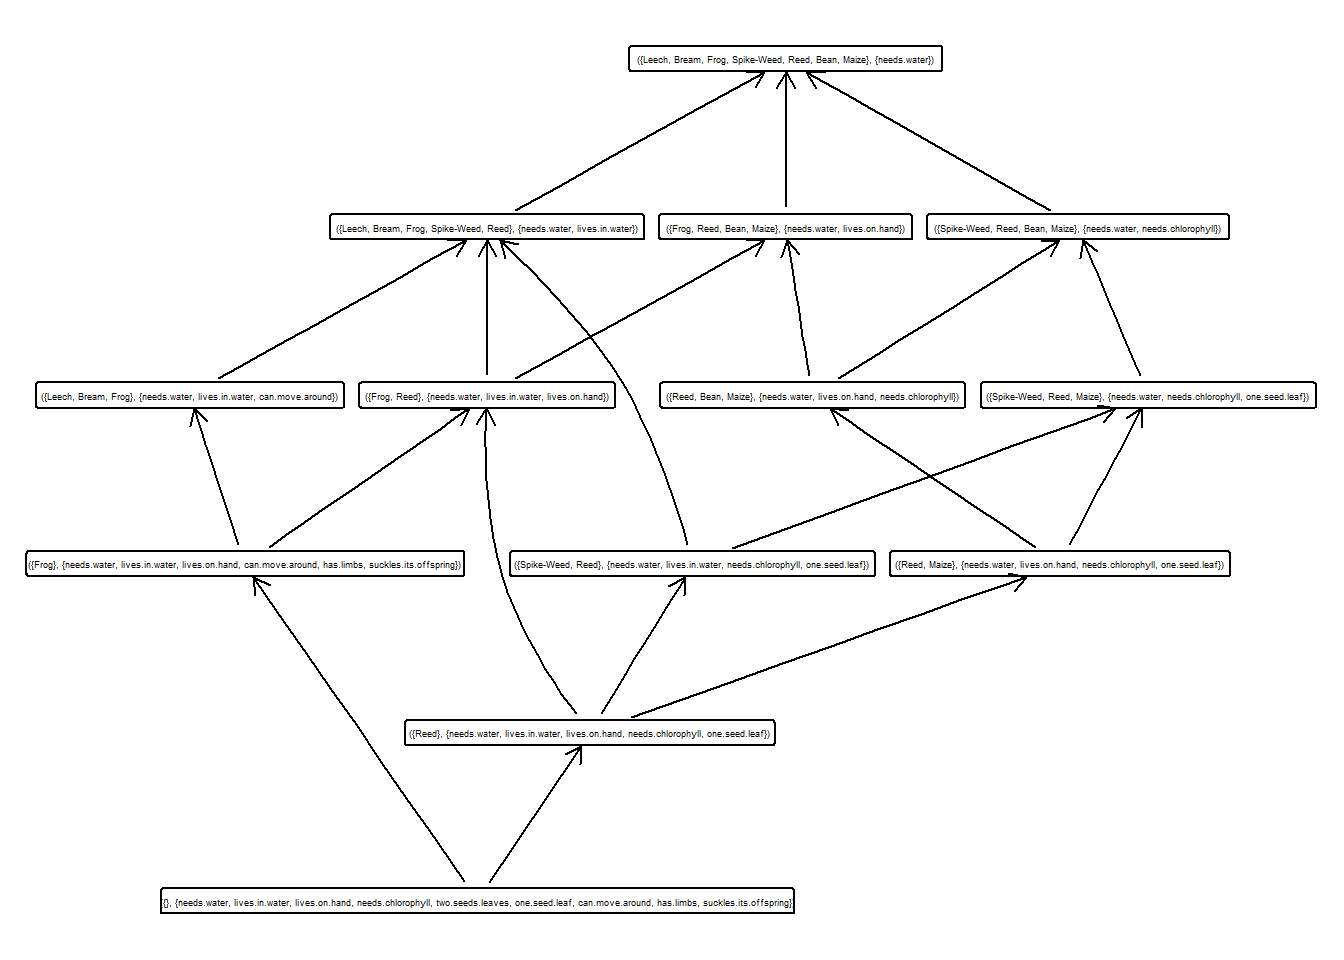
\includegraphics{book_LCC_files/figure-latex/unnamed-chunk-97-1.pdf}

¿De que tipo es el subretículo obtenido?.

\begin{Shaded}
\begin{Highlighting}[]
\FunctionTok{class}\NormalTok{(sublattice)}
\end{Highlighting}
\end{Shaded}

\begin{verbatim}
## [1] "ConceptLattice" "R6"
\end{verbatim}

Calcula el superior y el infimo de los conceptos calculados para fc\_ganter y lo mismo para el subretículo anterior. Visualizalos.

\begin{Shaded}
\begin{Highlighting}[]
\CommentTok{\#Supremo de los conceptos calculados para fc\_ganter}
\NormalTok{C }\OtherTok{\textless{}{-}}\NormalTok{ fc\_ganter}\SpecialCharTok{$}\NormalTok{concepts[}\DecValTok{1}\SpecialCharTok{:}\DecValTok{15}\NormalTok{]}
\NormalTok{C}
\end{Highlighting}
\end{Shaded}

\begin{verbatim}
## ({Leech, Bream, Frog, Spike-Weed, Reed, Bean, Maize}, {needs.water})
## ({Spike-Weed, Reed, Bean, Maize}, {needs.water, needs.chlorophyll})
## ({Spike-Weed, Reed, Maize}, {needs.water, needs.chlorophyll, one.seed.leaf})
## ({Frog, Reed, Bean, Maize}, {needs.water, lives.on.hand})
## ({Reed, Bean, Maize}, {needs.water, lives.on.hand, needs.chlorophyll})
## ({Reed, Maize}, {needs.water, lives.on.hand, needs.chlorophyll, one.seed.leaf})
## ({Bean}, {needs.water, lives.on.hand, needs.chlorophyll, two.seeds.leaves})
## ({Leech, Bream, Frog, Spike-Weed, Reed}, {needs.water, lives.in.water})
## ({Leech, Bream, Frog}, {needs.water, lives.in.water, can.move.around})
## ({Bream, Frog}, {needs.water, lives.in.water, can.move.around, has.limbs})
## ({Spike-Weed, Reed}, {needs.water, lives.in.water, needs.chlorophyll, one.seed.leaf})
## ({Frog, Reed}, {needs.water, lives.in.water, lives.on.hand})
## ({Frog}, {needs.water, lives.in.water, lives.on.hand, can.move.around, has.limbs,
##   suckles.its.offspring})
## ({Reed}, {needs.water, lives.in.water, lives.on.hand, needs.chlorophyll,
##   one.seed.leaf})
## ({}, {needs.water, lives.in.water, lives.on.hand, needs.chlorophyll,
##   two.seeds.leaves, one.seed.leaf, can.move.around, has.limbs,
##   suckles.its.offspring})
\end{verbatim}

\begin{Shaded}
\begin{Highlighting}[]
\NormalTok{fc\_ganter}\SpecialCharTok{$}\NormalTok{concepts}\SpecialCharTok{$}\FunctionTok{supremum}\NormalTok{(C)}
\end{Highlighting}
\end{Shaded}

\begin{verbatim}
## ({Leech, Bream, Frog, Spike-Weed, Reed, Bean, Maize}, {needs.water})
\end{verbatim}

\begin{Shaded}
\begin{Highlighting}[]
\CommentTok{\#Infimo de los conceptos calculados para fc\_ganter}
\NormalTok{fc\_ganter}\SpecialCharTok{$}\NormalTok{concepts}\SpecialCharTok{$}\FunctionTok{infimum}\NormalTok{(C)}
\end{Highlighting}
\end{Shaded}

\begin{verbatim}
## ({}, {needs.water, lives.in.water, lives.on.hand, needs.chlorophyll,
##   two.seeds.leaves, one.seed.leaf, can.move.around, has.limbs,
##   suckles.its.offspring})
\end{verbatim}

\begin{Shaded}
\begin{Highlighting}[]
\CommentTok{\#Supremo de los conceptos calculados para el subreticulo}
\NormalTok{C2 }\OtherTok{\textless{}{-}}\NormalTok{ sublattice[}\DecValTok{1}\SpecialCharTok{:}\DecValTok{13}\NormalTok{]}
\NormalTok{C2}
\end{Highlighting}
\end{Shaded}

\begin{verbatim}
## ({Leech, Bream, Frog, Spike-Weed, Reed, Bean, Maize}, {needs.water})
## ({Spike-Weed, Reed, Bean, Maize}, {needs.water, needs.chlorophyll})
## ({Spike-Weed, Reed, Maize}, {needs.water, needs.chlorophyll, one.seed.leaf})
## ({Frog, Reed, Bean, Maize}, {needs.water, lives.on.hand})
## ({Reed, Bean, Maize}, {needs.water, lives.on.hand, needs.chlorophyll})
## ({Reed, Maize}, {needs.water, lives.on.hand, needs.chlorophyll, one.seed.leaf})
## ({Leech, Bream, Frog, Spike-Weed, Reed}, {needs.water, lives.in.water})
## ({Leech, Bream, Frog}, {needs.water, lives.in.water, can.move.around})
## ({Spike-Weed, Reed}, {needs.water, lives.in.water, needs.chlorophyll, one.seed.leaf})
## ({Frog, Reed}, {needs.water, lives.in.water, lives.on.hand})
## ({Frog}, {needs.water, lives.in.water, lives.on.hand, can.move.around, has.limbs,
##   suckles.its.offspring})
## ({Reed}, {needs.water, lives.in.water, lives.on.hand, needs.chlorophyll,
##   one.seed.leaf})
## ({}, {needs.water, lives.in.water, lives.on.hand, needs.chlorophyll,
##   two.seeds.leaves, one.seed.leaf, can.move.around, has.limbs,
##   suckles.its.offspring})
\end{verbatim}

\begin{Shaded}
\begin{Highlighting}[]
\NormalTok{sublattice}\SpecialCharTok{$}\FunctionTok{supremum}\NormalTok{(C2)}
\end{Highlighting}
\end{Shaded}

\begin{verbatim}
## ({Leech, Bream, Frog, Spike-Weed, Reed, Bean, Maize}, {needs.water})
\end{verbatim}

\begin{Shaded}
\begin{Highlighting}[]
\CommentTok{\#Infimo de los conceptos calculados para el subreticulo}
\NormalTok{sublattice}\SpecialCharTok{$}\FunctionTok{infimum}\NormalTok{(C2)}
\end{Highlighting}
\end{Shaded}

\begin{verbatim}
## ({}, {needs.water, lives.in.water, lives.on.hand, needs.chlorophyll,
##   two.seeds.leaves, one.seed.leaf, can.move.around, has.limbs,
##   suckles.its.offspring})
\end{verbatim}

Grabar el objeto fc\_ganter en un fichero fc\_ganter.rds.

\begin{Shaded}
\begin{Highlighting}[]
\FunctionTok{saveRDS}\NormalTok{(fc\_ganter, }\AttributeTok{file =} \StringTok{"fc\_ganter.rds"}\NormalTok{)}
\end{Highlighting}
\end{Shaded}

Elimina la variable fc\_ganter. Carga otra vez en la variable del fichero anterior y comprueba que tenemos toda la información: atributos, conceptos, etc.

\begin{Shaded}
\begin{Highlighting}[]
\NormalTok{fc\_ganter }\OtherTok{\textless{}{-}} \ConstantTok{NULL}
\NormalTok{fc\_ganter }\OtherTok{\textless{}{-}} \FunctionTok{readRDS}\NormalTok{(}\AttributeTok{file=}\StringTok{"fc\_ganter.rds"}\NormalTok{)}
\end{Highlighting}
\end{Shaded}

Calcula lo siguientes conjuntos usando los métodos del paquete fcaR:

\begin{itemize}
\tightlist
\item
  \{Bean\}′
\item
  \{livesonland\}′
\item
  \{twoseedleaves\}′
\item
  \{Frog,Maize\}′
\item
  \{needschlorophylltoproducefood,canmovearound\}′
\item
  \{livesinwater,livesonland\}′
\item
  \{needschlorophylltoproducefood,canmovearound\}′
\end{itemize}

\begin{Shaded}
\begin{Highlighting}[]
\NormalTok{c1 }\OtherTok{\textless{}{-}}\NormalTok{ SparseSet}\SpecialCharTok{$}\FunctionTok{new}\NormalTok{(fc\_ganter}\SpecialCharTok{$}\NormalTok{objects)}
\NormalTok{c1}\SpecialCharTok{$}\FunctionTok{assign}\NormalTok{(}\AttributeTok{Bean=}\DecValTok{1}\NormalTok{)}
\NormalTok{fc\_ganter}\SpecialCharTok{$}\FunctionTok{intent}\NormalTok{(c1)}
\end{Highlighting}
\end{Shaded}

\begin{verbatim}
## {needs.water, lives.on.hand, needs.chlorophyll, two.seeds.leaves}
\end{verbatim}

\begin{Shaded}
\begin{Highlighting}[]
\NormalTok{c2 }\OtherTok{\textless{}{-}}\NormalTok{ SparseSet}\SpecialCharTok{$}\FunctionTok{new}\NormalTok{(fc\_ganter}\SpecialCharTok{$}\NormalTok{attributes)}
\NormalTok{c2}\SpecialCharTok{$}\FunctionTok{assign}\NormalTok{(}\AttributeTok{lives.on.hand=}\DecValTok{1}\NormalTok{)}
\NormalTok{fc\_ganter}\SpecialCharTok{$}\FunctionTok{extent}\NormalTok{(c2)}
\end{Highlighting}
\end{Shaded}

\begin{verbatim}
## {Frog, Reed, Bean, Maize}
\end{verbatim}

\begin{Shaded}
\begin{Highlighting}[]
\NormalTok{c3 }\OtherTok{\textless{}{-}}\NormalTok{ SparseSet}\SpecialCharTok{$}\FunctionTok{new}\NormalTok{(fc\_ganter}\SpecialCharTok{$}\NormalTok{attributes)}
\NormalTok{c3}\SpecialCharTok{$}\FunctionTok{assign}\NormalTok{(}\AttributeTok{two.seed.leaves=}\DecValTok{1}\NormalTok{)}
\NormalTok{fc\_ganter}\SpecialCharTok{$}\FunctionTok{extent}\NormalTok{(c3)}
\end{Highlighting}
\end{Shaded}

\begin{verbatim}
## {Leech, Bream, Frog, Spike-Weed, Reed, Bean, Maize}
\end{verbatim}

\begin{Shaded}
\begin{Highlighting}[]
\NormalTok{c4 }\OtherTok{\textless{}{-}}\NormalTok{ SparseSet}\SpecialCharTok{$}\FunctionTok{new}\NormalTok{(fc\_ganter}\SpecialCharTok{$}\NormalTok{objects)}
\NormalTok{c4}\SpecialCharTok{$}\FunctionTok{assign}\NormalTok{(}\AttributeTok{Frog=}\DecValTok{1}\NormalTok{, }\AttributeTok{Maize=}\DecValTok{1}\NormalTok{)}
\NormalTok{fc\_ganter}\SpecialCharTok{$}\FunctionTok{intent}\NormalTok{(c4)}
\end{Highlighting}
\end{Shaded}

\begin{verbatim}
## {needs.water, lives.on.hand}
\end{verbatim}

\begin{Shaded}
\begin{Highlighting}[]
\NormalTok{c5 }\OtherTok{\textless{}{-}}\NormalTok{ SparseSet}\SpecialCharTok{$}\FunctionTok{new}\NormalTok{(fc\_ganter}\SpecialCharTok{$}\NormalTok{attributes)}
\NormalTok{c5}\SpecialCharTok{$}\FunctionTok{assign}\NormalTok{(}\AttributeTok{needs.chlorophyll=}\DecValTok{1}\NormalTok{,}\AttributeTok{can.move.around=}\DecValTok{1}\NormalTok{)}
\NormalTok{fc\_ganter}\SpecialCharTok{$}\FunctionTok{extent}\NormalTok{(c5)}
\end{Highlighting}
\end{Shaded}

\begin{verbatim}
## {}
\end{verbatim}

\begin{Shaded}
\begin{Highlighting}[]
\NormalTok{c6 }\OtherTok{\textless{}{-}}\NormalTok{ SparseSet}\SpecialCharTok{$}\FunctionTok{new}\NormalTok{(fc\_ganter}\SpecialCharTok{$}\NormalTok{attributes)}
\NormalTok{c6}\SpecialCharTok{$}\FunctionTok{assign}\NormalTok{(}\AttributeTok{lives.in.water=}\DecValTok{1}\NormalTok{,}\AttributeTok{lives.on.hand=}\DecValTok{1}\NormalTok{)}
\NormalTok{fc\_ganter}\SpecialCharTok{$}\FunctionTok{extent}\NormalTok{(c6)}
\end{Highlighting}
\end{Shaded}

\begin{verbatim}
## {Frog, Reed}
\end{verbatim}

\hypertarget{tutorial-ganter-implications}{%
\section{Tutorial Ganter (Implications)}\label{tutorial-ganter-implications}}

Introduce órdenes para cargar los paquetes necesarios para trabajar con FCA:

\begin{Shaded}
\begin{Highlighting}[]
\FunctionTok{library}\NormalTok{(}\StringTok{\textquotesingle{}fcaR\textquotesingle{}}\NormalTok{)}
\FunctionTok{library}\NormalTok{(arules)}
\end{Highlighting}
\end{Shaded}

\begin{Shaded}
\begin{Highlighting}[]
\NormalTok{dataset\_ganter }\OtherTok{\textless{}{-}} \FunctionTok{read.csv}\NormalTok{(}\StringTok{"contextformal\_tutorialGanter.csv"}\NormalTok{, }\AttributeTok{sep=}\StringTok{";"}\NormalTok{)}
\FunctionTok{View}\NormalTok{(dataset\_ganter)}
\FunctionTok{rownames}\NormalTok{(dataset\_ganter) }\OtherTok{\textless{}{-}}\NormalTok{ dataset\_ganter[[}\DecValTok{1}\NormalTok{]]}

\NormalTok{dataset\_ganter[[}\DecValTok{1}\NormalTok{]] }\OtherTok{\textless{}{-}} \ConstantTok{NULL}

\NormalTok{dataset\_ganter}
\end{Highlighting}
\end{Shaded}

\begin{verbatim}
##            needs.water lives.in.water lives.on.hand needs.chlorophyll
## Leech                1              1             0                 0
## Bream                1              1             0                 0
## Frog                 1              1             1                 0
## Spike-Weed           1              1             0                 1
## Reed                 1              1             1                 1
## Bean                 1              0             1                 1
## Maize                1              0             1                 1
##            two.seeds.leaves one.seed.leaf can.move.around has.limbs
## Leech                     0             0               1         0
## Bream                     0             0               1         1
## Frog                      0             0               1         1
## Spike-Weed                0             1               0         0
## Reed                      0             1               0         0
## Bean                      1             0               0         0
## Maize                     0             1               0         0
##            suckles.its.offspring
## Leech                          0
## Bream                          0
## Frog                           1
## Spike-Weed                     0
## Reed                           0
## Bean                           0
## Maize                          0
\end{verbatim}

\begin{Shaded}
\begin{Highlighting}[]
\NormalTok{fc\_ganter }\OtherTok{\textless{}{-}}\NormalTok{ FormalContext}\SpecialCharTok{$}\FunctionTok{new}\NormalTok{(dataset\_ganter)}

\FunctionTok{plot}\NormalTok{(fc\_ganter)}
\end{Highlighting}
\end{Shaded}

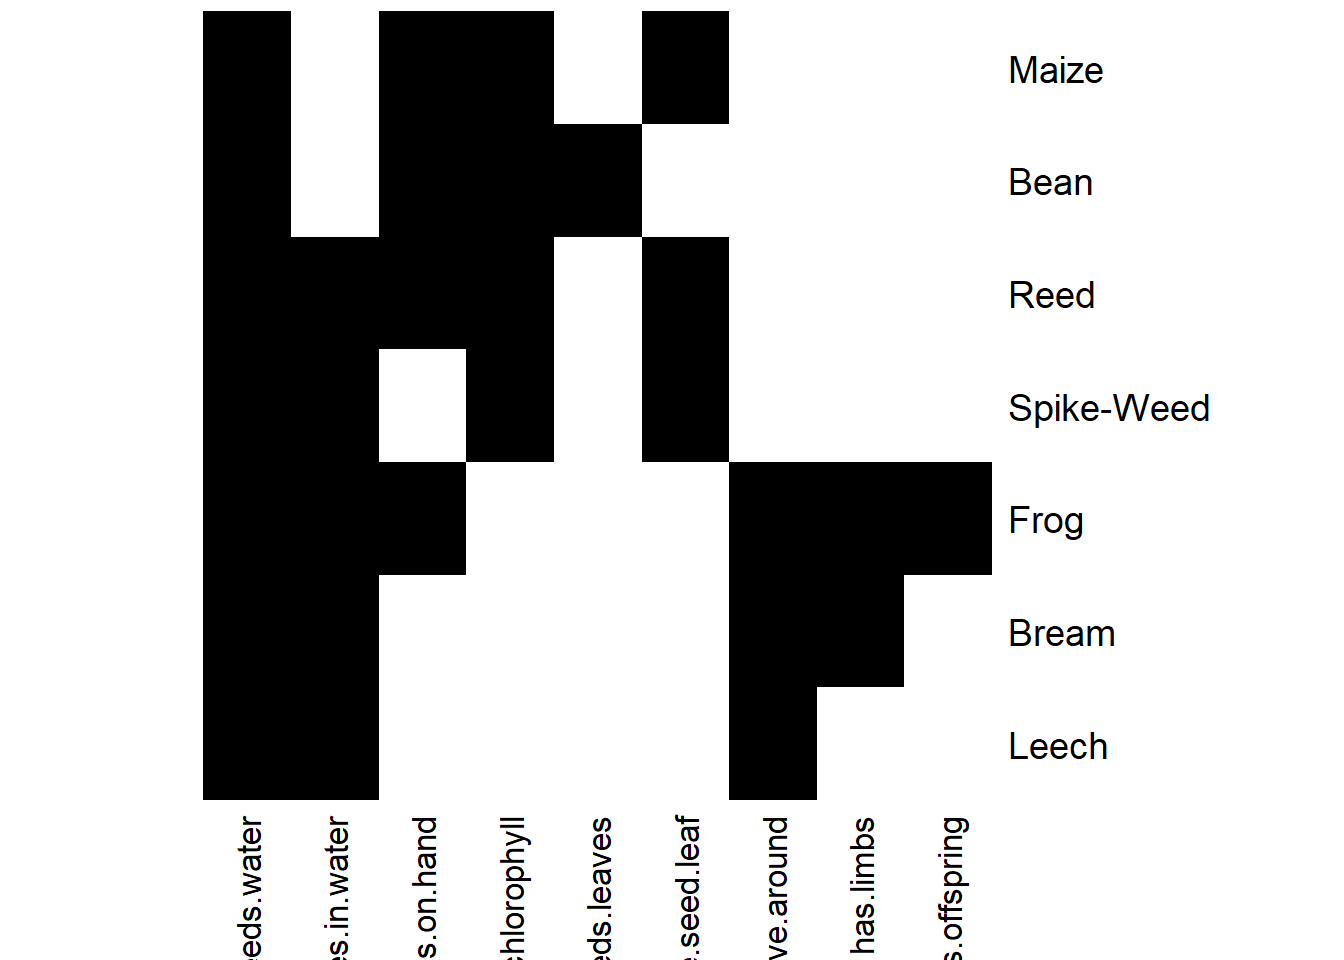
\includegraphics{book_LCC_files/figure-latex/unnamed-chunk-110-1.pdf}

\begin{Shaded}
\begin{Highlighting}[]
\FunctionTok{print}\NormalTok{(fc\_ganter)}
\end{Highlighting}
\end{Shaded}

\begin{verbatim}
## FormalContext with 7 objects and 9 attributes.
##               needs.water   lives.in.water   lives.on.hand   needs.chlorophyll  
##        Leech       X              X                                             
##        Bream       X              X                                             
##         Frog       X              X                X                            
##   Spike-Weed       X              X                                  X          
##         Reed       X              X                X                 X          
##         Bean       X                               X                 X          
##        Maize       X                               X                 X          
## Other attributes are: two.seeds.leaves, one.seed.leaf, can.move.around,
## has.limbs, suckles.its.offspring
\end{verbatim}

Calcula las implicaciones del contexto y muestra las implicaciones en pantalla

\begin{Shaded}
\begin{Highlighting}[]
\NormalTok{fc\_ganter}\SpecialCharTok{$}\FunctionTok{find\_implications}\NormalTok{()}
\NormalTok{fc\_ganter}\SpecialCharTok{$}\NormalTok{implications}
\end{Highlighting}
\end{Shaded}

\begin{verbatim}
## Implication set with 10 implications.
## Rule 1: {} -> {needs.water}
## Rule 2: {needs.water, suckles.its.offspring} -> {lives.in.water,
##   lives.on.hand, can.move.around, has.limbs}
## Rule 3: {needs.water, has.limbs} -> {lives.in.water, can.move.around}
## Rule 4: {needs.water, can.move.around} -> {lives.in.water}
## Rule 5: {needs.water, one.seed.leaf} -> {needs.chlorophyll}
## Rule 6: {needs.water, two.seeds.leaves} -> {lives.on.hand,
##   needs.chlorophyll}
## Rule 7: {needs.water, lives.on.hand, needs.chlorophyll,
##   two.seeds.leaves, one.seed.leaf} -> {lives.in.water,
##   can.move.around, has.limbs, suckles.its.offspring}
## Rule 8: {needs.water, lives.in.water, needs.chlorophyll} ->
##   {one.seed.leaf}
## Rule 9: {needs.water, lives.in.water, needs.chlorophyll,
##   one.seed.leaf, can.move.around} -> {lives.on.hand, two.seeds.leaves,
##   has.limbs, suckles.its.offspring}
## Rule 10: {needs.water, lives.in.water, lives.on.hand, can.move.around}
##   -> {has.limbs, suckles.its.offspring}
\end{verbatim}

¿Cuantas implicaciones se han extraido?

\begin{Shaded}
\begin{Highlighting}[]
\NormalTok{fc\_ganter}\SpecialCharTok{$}\NormalTok{implications}\SpecialCharTok{$}\FunctionTok{cardinality}\NormalTok{()}
\end{Highlighting}
\end{Shaded}

\begin{verbatim}
## [1] 10
\end{verbatim}

Calcula el tamaño de las implicaciones y la media de la parte y derecha de dichas implicaciones.

\begin{Shaded}
\begin{Highlighting}[]
\NormalTok{tam }\OtherTok{\textless{}{-}}\NormalTok{ fc\_ganter}\SpecialCharTok{$}\NormalTok{implications}\SpecialCharTok{$}\FunctionTok{size}\NormalTok{()}
\FunctionTok{colMeans}\NormalTok{(tam)}
\end{Highlighting}
\end{Shaded}

\begin{verbatim}
## LHS RHS 
## 2.7 2.2
\end{verbatim}

Aplica las reglas de la lógica de simplificación. ¿Cuantas implicaciones han aparecido tras aplicar la lógica?

\begin{Shaded}
\begin{Highlighting}[]
\NormalTok{fc\_ganter}\SpecialCharTok{$}\NormalTok{implications}\SpecialCharTok{$}\FunctionTok{apply\_rules}\NormalTok{(}\AttributeTok{rules =} \StringTok{"simplification"}\NormalTok{)}
\end{Highlighting}
\end{Shaded}

\begin{verbatim}
## Processing batch
\end{verbatim}

\begin{verbatim}
## --> Simplification: from 10 to 10 in 0.12 secs.
\end{verbatim}

\begin{verbatim}
## Batch took 0.12 secs.
\end{verbatim}

\begin{Shaded}
\begin{Highlighting}[]
\NormalTok{fc\_ganter}\SpecialCharTok{$}\NormalTok{implications}
\end{Highlighting}
\end{Shaded}

\begin{verbatim}
## Implication set with 10 implications.
## Rule 1: {} -> {needs.water}
## Rule 2: {suckles.its.offspring} -> {lives.in.water, lives.on.hand,
##   can.move.around, has.limbs}
## Rule 3: {has.limbs} -> {lives.in.water, can.move.around}
## Rule 4: {can.move.around} -> {lives.in.water}
## Rule 5: {one.seed.leaf} -> {needs.chlorophyll}
## Rule 6: {two.seeds.leaves} -> {lives.on.hand, needs.chlorophyll}
## Rule 7: {two.seeds.leaves, one.seed.leaf} -> {lives.in.water,
##   can.move.around, has.limbs, suckles.its.offspring}
## Rule 8: {lives.in.water, needs.chlorophyll} -> {one.seed.leaf}
## Rule 9: {one.seed.leaf, can.move.around} -> {lives.on.hand,
##   two.seeds.leaves, has.limbs, suckles.its.offspring}
## Rule 10: {lives.on.hand, can.move.around} -> {has.limbs,
##   suckles.its.offspring}
\end{verbatim}

\begin{Shaded}
\begin{Highlighting}[]
\NormalTok{fc\_ganter}\SpecialCharTok{$}\NormalTok{implications}\SpecialCharTok{$}\FunctionTok{cardinality}\NormalTok{()}
\end{Highlighting}
\end{Shaded}

\begin{verbatim}
## [1] 10
\end{verbatim}

Eliminar la redundancia en el conjunto de implicaciones. ¿Cuantas implicaciones han aparecido tras aplicar la lógica?

\begin{Shaded}
\begin{Highlighting}[]
\NormalTok{fc\_ganter}\SpecialCharTok{$}\NormalTok{implications}\SpecialCharTok{$}\FunctionTok{apply\_rules}\NormalTok{(}\AttributeTok{rules =} \FunctionTok{c}\NormalTok{(}\StringTok{"composition"}\NormalTok{,}\StringTok{"generalization"}\NormalTok{,}\StringTok{"simplification"}\NormalTok{))                                   }
\end{Highlighting}
\end{Shaded}

\begin{verbatim}
## Processing batch
\end{verbatim}

\begin{verbatim}
## --> Composition: from 10 to 10 in 0 secs.
\end{verbatim}

\begin{verbatim}
## --> Generalization: from 10 to 10 in 0.02 secs.
\end{verbatim}

\begin{verbatim}
## --> Simplification: from 10 to 10 in 0.03 secs.
\end{verbatim}

\begin{verbatim}
## Batch took 0.05 secs.
\end{verbatim}

\begin{Shaded}
\begin{Highlighting}[]
\NormalTok{fc\_ganter}\SpecialCharTok{$}\NormalTok{implications}
\end{Highlighting}
\end{Shaded}

\begin{verbatim}
## Implication set with 10 implications.
## Rule 1: {} -> {needs.water}
## Rule 2: {suckles.its.offspring} -> {lives.in.water, lives.on.hand,
##   can.move.around, has.limbs}
## Rule 3: {has.limbs} -> {lives.in.water, can.move.around}
## Rule 4: {can.move.around} -> {lives.in.water}
## Rule 5: {one.seed.leaf} -> {needs.chlorophyll}
## Rule 6: {two.seeds.leaves} -> {lives.on.hand, needs.chlorophyll}
## Rule 7: {two.seeds.leaves, one.seed.leaf} -> {lives.in.water,
##   can.move.around, has.limbs, suckles.its.offspring}
## Rule 8: {lives.in.water, needs.chlorophyll} -> {one.seed.leaf}
## Rule 9: {one.seed.leaf, can.move.around} -> {lives.on.hand,
##   two.seeds.leaves, has.limbs, suckles.its.offspring}
## Rule 10: {lives.on.hand, can.move.around} -> {has.limbs,
##   suckles.its.offspring}
\end{verbatim}

\begin{Shaded}
\begin{Highlighting}[]
\NormalTok{fc\_ganter}\SpecialCharTok{$}\NormalTok{implications}\SpecialCharTok{$}\FunctionTok{cardinality}\NormalTok{()}
\end{Highlighting}
\end{Shaded}

\begin{verbatim}
## [1] 10
\end{verbatim}

Calcular el cierre de los atributos needs.water, one.seed.leaf.

\begin{Shaded}
\begin{Highlighting}[]
\NormalTok{S }\OtherTok{\textless{}{-}}\NormalTok{ SparseSet}\SpecialCharTok{$}\FunctionTok{new}\NormalTok{(}\AttributeTok{attributes =}\NormalTok{ fc\_ganter}\SpecialCharTok{$}\NormalTok{attributes)}
\NormalTok{S}\SpecialCharTok{$}\FunctionTok{assign}\NormalTok{(}\AttributeTok{needs.water=}\DecValTok{1}\NormalTok{,}\AttributeTok{one.seed.leaf=}\DecValTok{1}\NormalTok{)}
\NormalTok{S}
\end{Highlighting}
\end{Shaded}

\begin{verbatim}
## {needs.water, one.seed.leaf}
\end{verbatim}

\begin{Shaded}
\begin{Highlighting}[]
\NormalTok{fc\_ganter}\SpecialCharTok{$}\NormalTok{implications}\SpecialCharTok{$}\FunctionTok{closure}\NormalTok{(S)}
\end{Highlighting}
\end{Shaded}

\begin{verbatim}
## $closure
## {needs.water, needs.chlorophyll, one.seed.leaf}
\end{verbatim}

Copia (clona) el conjunto fc\_ganter en una variable fc1.

\begin{Shaded}
\begin{Highlighting}[]
\NormalTok{fc1 }\OtherTok{\textless{}{-}}\NormalTok{ fc\_ganter}\SpecialCharTok{$}\FunctionTok{clone}\NormalTok{()}
\FunctionTok{plot}\NormalTok{(fc1)}
\end{Highlighting}
\end{Shaded}

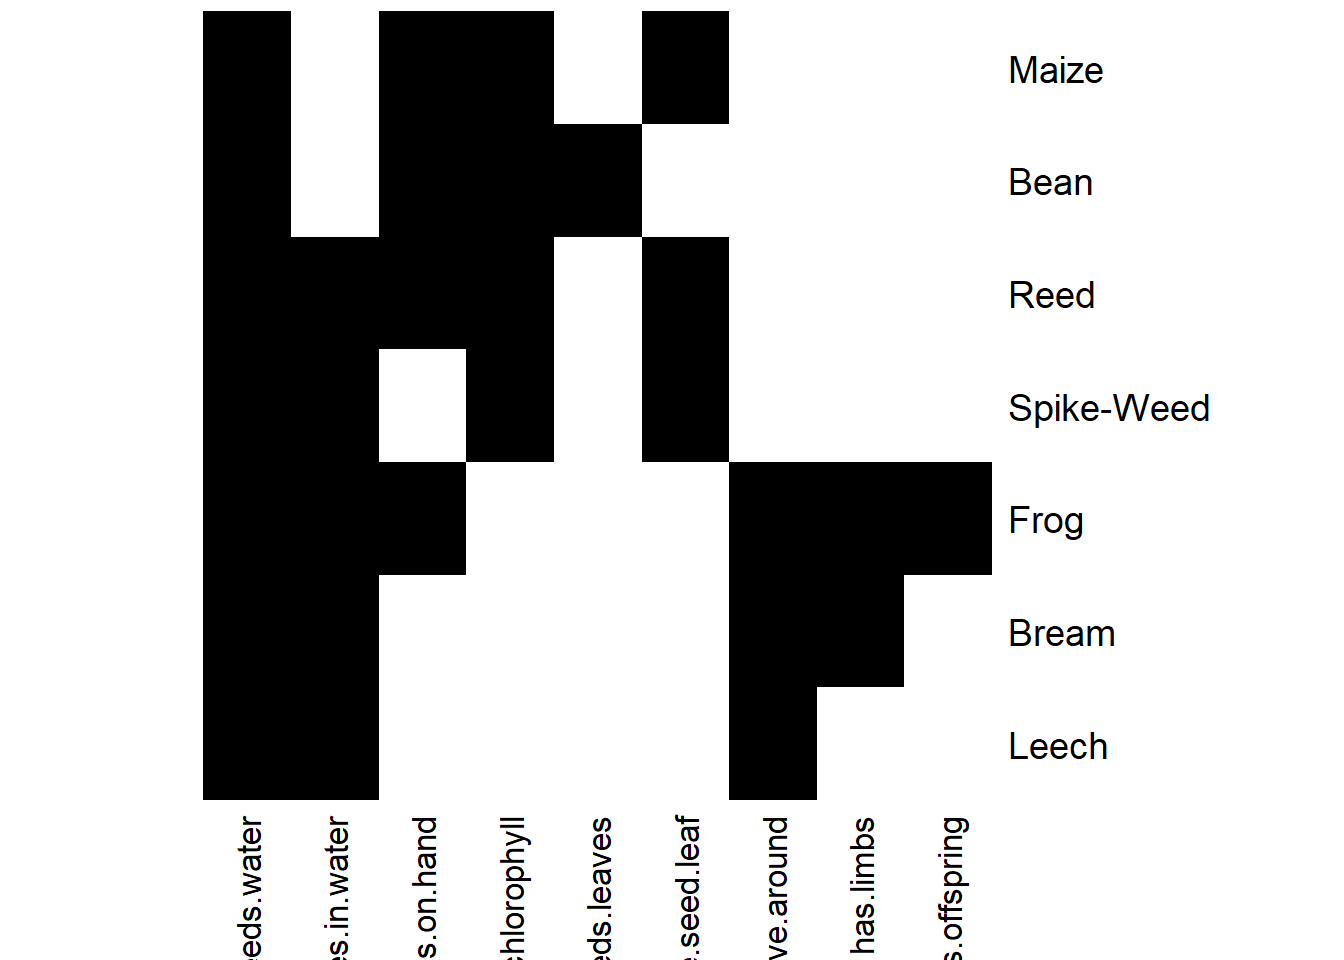
\includegraphics{book_LCC_files/figure-latex/unnamed-chunk-122-1.pdf}

\begin{Shaded}
\begin{Highlighting}[]
\NormalTok{fc1}\SpecialCharTok{$}\NormalTok{implications}
\end{Highlighting}
\end{Shaded}

\begin{verbatim}
## Implication set with 10 implications.
## Rule 1: {} -> {needs.water}
## Rule 2: {suckles.its.offspring} -> {lives.in.water, lives.on.hand,
##   can.move.around, has.limbs}
## Rule 3: {has.limbs} -> {lives.in.water, can.move.around}
## Rule 4: {can.move.around} -> {lives.in.water}
## Rule 5: {one.seed.leaf} -> {needs.chlorophyll}
## Rule 6: {two.seeds.leaves} -> {lives.on.hand, needs.chlorophyll}
## Rule 7: {two.seeds.leaves, one.seed.leaf} -> {lives.in.water,
##   can.move.around, has.limbs, suckles.its.offspring}
## Rule 8: {lives.in.water, needs.chlorophyll} -> {one.seed.leaf}
## Rule 9: {one.seed.leaf, can.move.around} -> {lives.on.hand,
##   two.seeds.leaves, has.limbs, suckles.its.offspring}
## Rule 10: {lives.on.hand, can.move.around} -> {has.limbs,
##   suckles.its.offspring}
\end{verbatim}

Elimina la implicación que está en la primera posición

\begin{Shaded}
\begin{Highlighting}[]
\NormalTok{fc1}\SpecialCharTok{$}\NormalTok{implications }\OtherTok{\textless{}{-}}\NormalTok{ fc1}\SpecialCharTok{$}\NormalTok{implications[}\SpecialCharTok{{-}}\DecValTok{1}\NormalTok{]}
\NormalTok{fc1}\SpecialCharTok{$}\NormalTok{implications}
\end{Highlighting}
\end{Shaded}

\begin{verbatim}
## Implication set with 9 implications.
## Rule 1: {suckles.its.offspring} -> {lives.in.water, lives.on.hand,
##   can.move.around, has.limbs}
## Rule 2: {has.limbs} -> {lives.in.water, can.move.around}
## Rule 3: {can.move.around} -> {lives.in.water}
## Rule 4: {one.seed.leaf} -> {needs.chlorophyll}
## Rule 5: {two.seeds.leaves} -> {lives.on.hand, needs.chlorophyll}
## Rule 6: {two.seeds.leaves, one.seed.leaf} -> {lives.in.water,
##   can.move.around, has.limbs, suckles.its.offspring}
## Rule 7: {lives.in.water, needs.chlorophyll} -> {one.seed.leaf}
## Rule 8: {one.seed.leaf, can.move.around} -> {lives.on.hand,
##   two.seeds.leaves, has.limbs, suckles.its.offspring}
## Rule 9: {lives.on.hand, can.move.around} -> {has.limbs,
##   suckles.its.offspring}
\end{verbatim}

Extrae de todas las implicaciones la que tengan en el lado izquierdo de la implicación el atributo one.seed.leaf.

\begin{Shaded}
\begin{Highlighting}[]
\NormalTok{impIzd }\OtherTok{\textless{}{-}}\NormalTok{ fc1}\SpecialCharTok{$}\NormalTok{implications}\SpecialCharTok{$}\FunctionTok{filter}\NormalTok{(}\AttributeTok{lhs=}\StringTok{"one.seed.leaf"}\NormalTok{)}
\NormalTok{impIzd}
\end{Highlighting}
\end{Shaded}

\begin{verbatim}
## Implication set with 3 implications.
## Rule 1: {one.seed.leaf} -> {needs.chlorophyll}
## Rule 2: {two.seeds.leaves, one.seed.leaf} -> {lives.in.water,
##   can.move.around, has.limbs, suckles.its.offspring}
## Rule 3: {one.seed.leaf, can.move.around} -> {lives.on.hand,
##   two.seeds.leaves, has.limbs, suckles.its.offspring}
\end{verbatim}

Obtén los atributos que aparezcan en todas las implicaciones.

\begin{Shaded}
\begin{Highlighting}[]
\NormalTok{impIzd}\SpecialCharTok{$}\FunctionTok{get\_attributes}\NormalTok{()}
\end{Highlighting}
\end{Shaded}

\begin{verbatim}
## [1] "needs.water"           "lives.in.water"        "lives.on.hand"        
## [4] "needs.chlorophyll"     "two.seeds.leaves"      "one.seed.leaf"        
## [7] "can.move.around"       "has.limbs"             "suckles.its.offspring"
\end{verbatim}

Calcula el soporte de la implicación 3

\begin{Shaded}
\begin{Highlighting}[]
\NormalTok{impIzd}\SpecialCharTok{$}\FunctionTok{support}\NormalTok{()[}\DecValTok{3}\NormalTok{]}
\end{Highlighting}
\end{Shaded}

\begin{verbatim}
## [1] 0.3333333
\end{verbatim}

\hypertarget{regresiuxf3n}{%
\chapter{Regresión}\label{regresiuxf3n}}

\begin{Shaded}
\begin{Highlighting}[]
\FunctionTok{library}\NormalTok{(dplyr)}
\FunctionTok{library}\NormalTok{(readr)}
\FunctionTok{library}\NormalTok{(ggplot2)}
\FunctionTok{library}\NormalTok{(GGally)}
\end{Highlighting}
\end{Shaded}

\begin{verbatim}
## Warning: package 'GGally' was built under R version 4.0.5
\end{verbatim}

\begin{verbatim}
## Registered S3 method overwritten by 'GGally':
##   method from   
##   +.gg   ggplot2
\end{verbatim}

\begin{Shaded}
\begin{Highlighting}[]
\NormalTok{riesgos }\OtherTok{\textless{}{-}} \FunctionTok{read\_csv}\NormalTok{(}\StringTok{"riesgos.csv"}\NormalTok{)}
\end{Highlighting}
\end{Shaded}

\begin{verbatim}
## 
## -- Column specification --------------------------------------------------------
## cols(
##   edad = col_double(),
##   sexo = col_character(),
##   bmi = col_double(),
##   hijos = col_double(),
##   fumador = col_character(),
##   region = col_character(),
##   gastos = col_double()
## )
\end{verbatim}

\begin{Shaded}
\begin{Highlighting}[]
\FunctionTok{head}\NormalTok{(riesgos)}
\end{Highlighting}
\end{Shaded}

\begin{verbatim}
## # A tibble: 6 x 7
##    edad sexo     bmi hijos fumador region    gastos
##   <dbl> <chr>  <dbl> <dbl> <chr>   <chr>      <dbl>
## 1    19 mujer   27.9     0 si      Andalucía 16885.
## 2    18 hombre  33.8     1 no      Murcia     1726.
## 3    28 hombre  33       3 no      Murcia     4449.
## 4    33 hombre  22.7     0 no      Madrid    21984.
## 5    32 hombre  28.9     0 no      Madrid     3867.
## 6    31 mujer   25.7     0 no      Murcia     3757.
\end{verbatim}

\begin{Shaded}
\begin{Highlighting}[]
\FunctionTok{glimpse}\NormalTok{(riesgos)}
\end{Highlighting}
\end{Shaded}

\begin{verbatim}
## Rows: 1,338
## Columns: 7
## $ edad    <dbl> 19, 18, 28, 33, 32, 31, 46, 37, 37, 60, 25, 62, 23, 56, 27, 19~
## $ sexo    <chr> "mujer", "hombre", "hombre", "hombre", "hombre", "mujer", "muj~
## $ bmi     <dbl> 27.900, 33.770, 33.000, 22.705, 28.880, 25.740, 33.440, 27.740~
## $ hijos   <dbl> 0, 1, 3, 0, 0, 0, 1, 3, 2, 0, 0, 0, 0, 0, 0, 1, 1, 0, 0, 0, 0,~
## $ fumador <chr> "si", "no", "no", "no", "no", "no", "no", "no", "no", "no", "n~
## $ region  <chr> "Andalucía", "Murcia", "Murcia", "Madrid", "Madrid", "Murcia",~
## $ gastos  <dbl> 16884.924, 1725.552, 4449.462, 21984.471, 3866.855, 3756.622, ~
\end{verbatim}

\begin{Shaded}
\begin{Highlighting}[]
\CommentTok{\#Al trabajar con este dataset podemos encontrarnos con el problema de que algunas columnas son de tipo char y por tanto no podemos trabajar con ellas}
\end{Highlighting}
\end{Shaded}

\begin{Shaded}
\begin{Highlighting}[]
\FunctionTok{summary}\NormalTok{(riesgos)}
\end{Highlighting}
\end{Shaded}

\begin{verbatim}
##       edad           sexo                bmi            hijos      
##  Min.   :18.00   Length:1338        Min.   :15.96   Min.   :0.000  
##  1st Qu.:27.00   Class :character   1st Qu.:26.30   1st Qu.:0.000  
##  Median :39.00   Mode  :character   Median :30.40   Median :1.000  
##  Mean   :39.21                      Mean   :30.66   Mean   :1.095  
##  3rd Qu.:51.00                      3rd Qu.:34.69   3rd Qu.:2.000  
##  Max.   :64.00                      Max.   :53.13   Max.   :5.000  
##    fumador             region              gastos     
##  Length:1338        Length:1338        Min.   : 1122  
##  Class :character   Class :character   1st Qu.: 4740  
##  Mode  :character   Mode  :character   Median : 9382  
##                                        Mean   :13270  
##                                        3rd Qu.:16640  
##                                        Max.   :63770
\end{verbatim}

\begin{Shaded}
\begin{Highlighting}[]
\CommentTok{\#Como podemos obsevar, de las columnas sexo, fumador y región no podemos extraer información ninguna si usamos summary, por lo tanto no usaríamos dichas columnas}
\end{Highlighting}
\end{Shaded}

\begin{Shaded}
\begin{Highlighting}[]
\NormalTok{copia\_riesgos }\OtherTok{\textless{}{-}}\NormalTok{ riesgos }\SpecialCharTok{\%\textgreater{}\%} \FunctionTok{select}\NormalTok{(edad,bmi,hijos,gastos)}
\FunctionTok{pairs}\NormalTok{(copia\_riesgos)}
\end{Highlighting}
\end{Shaded}

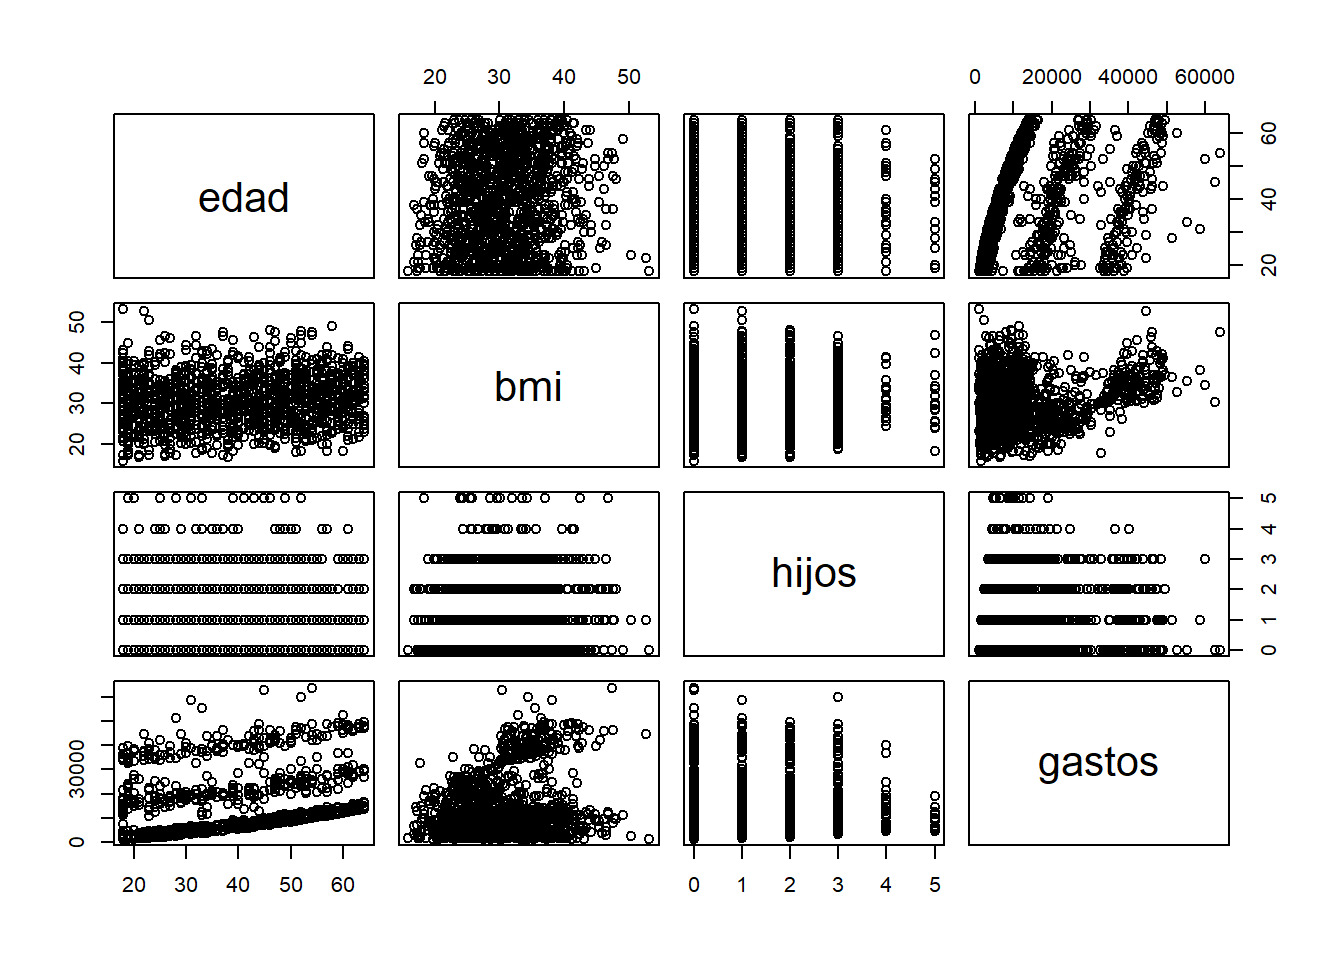
\includegraphics{book_LCC_files/figure-latex/unnamed-chunk-131-1.pdf}

\begin{Shaded}
\begin{Highlighting}[]
\CommentTok{\#Al ejecutar pairs se muestran las matrices de dispersión que representan las relaciones entre pares de variables cuantitativas. Por ejemplo, se puede observar en la matriz que relaciona la edad con los gastos que estos últimos aumentan respecto a la edad.}
\end{Highlighting}
\end{Shaded}

\begin{Shaded}
\begin{Highlighting}[]
\FunctionTok{ggplot}\NormalTok{(}\AttributeTok{data =}\NormalTok{ copia\_riesgos, }\AttributeTok{mapping =} \FunctionTok{aes}\NormalTok{(}\AttributeTok{x =}\NormalTok{ edad, }\AttributeTok{y =}\NormalTok{ gastos)) }\SpecialCharTok{+}
\FunctionTok{geom\_point}\NormalTok{(}\AttributeTok{color =} \StringTok{"firebrick"}\NormalTok{, }\AttributeTok{size =} \DecValTok{2}\NormalTok{) }\SpecialCharTok{+}
\FunctionTok{labs}\NormalTok{(}\AttributeTok{title =} \StringTok{"Diagrama de dispersión"}\NormalTok{, }\AttributeTok{x =} \StringTok{"Edad"}\NormalTok{, }\AttributeTok{y =} \StringTok{"Gastos"}\NormalTok{) }\SpecialCharTok{+}
\FunctionTok{theme\_bw}\NormalTok{() }\SpecialCharTok{+}
\FunctionTok{theme}\NormalTok{(}\AttributeTok{plot.title =} \FunctionTok{element\_text}\NormalTok{(}\AttributeTok{hjust =} \FloatTok{0.5}\NormalTok{))}
\end{Highlighting}
\end{Shaded}

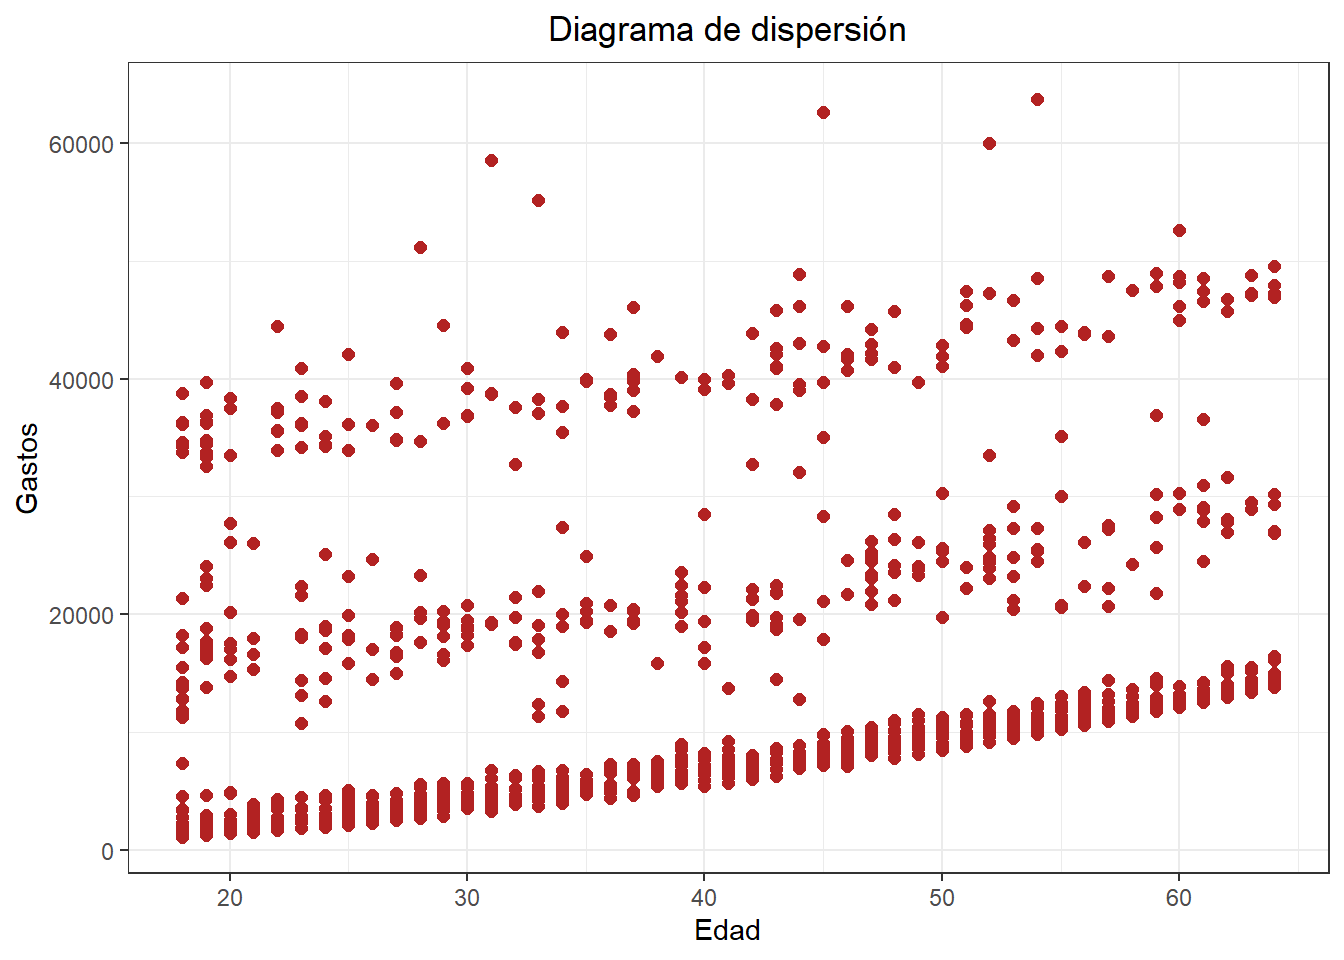
\includegraphics{book_LCC_files/figure-latex/unnamed-chunk-132-1.pdf}

Histograma del atributo gastos

\begin{Shaded}
\begin{Highlighting}[]
\FunctionTok{hist}\NormalTok{(}\AttributeTok{x=}\NormalTok{copia\_riesgos}\SpecialCharTok{$}\NormalTok{gastos )}
\end{Highlighting}
\end{Shaded}

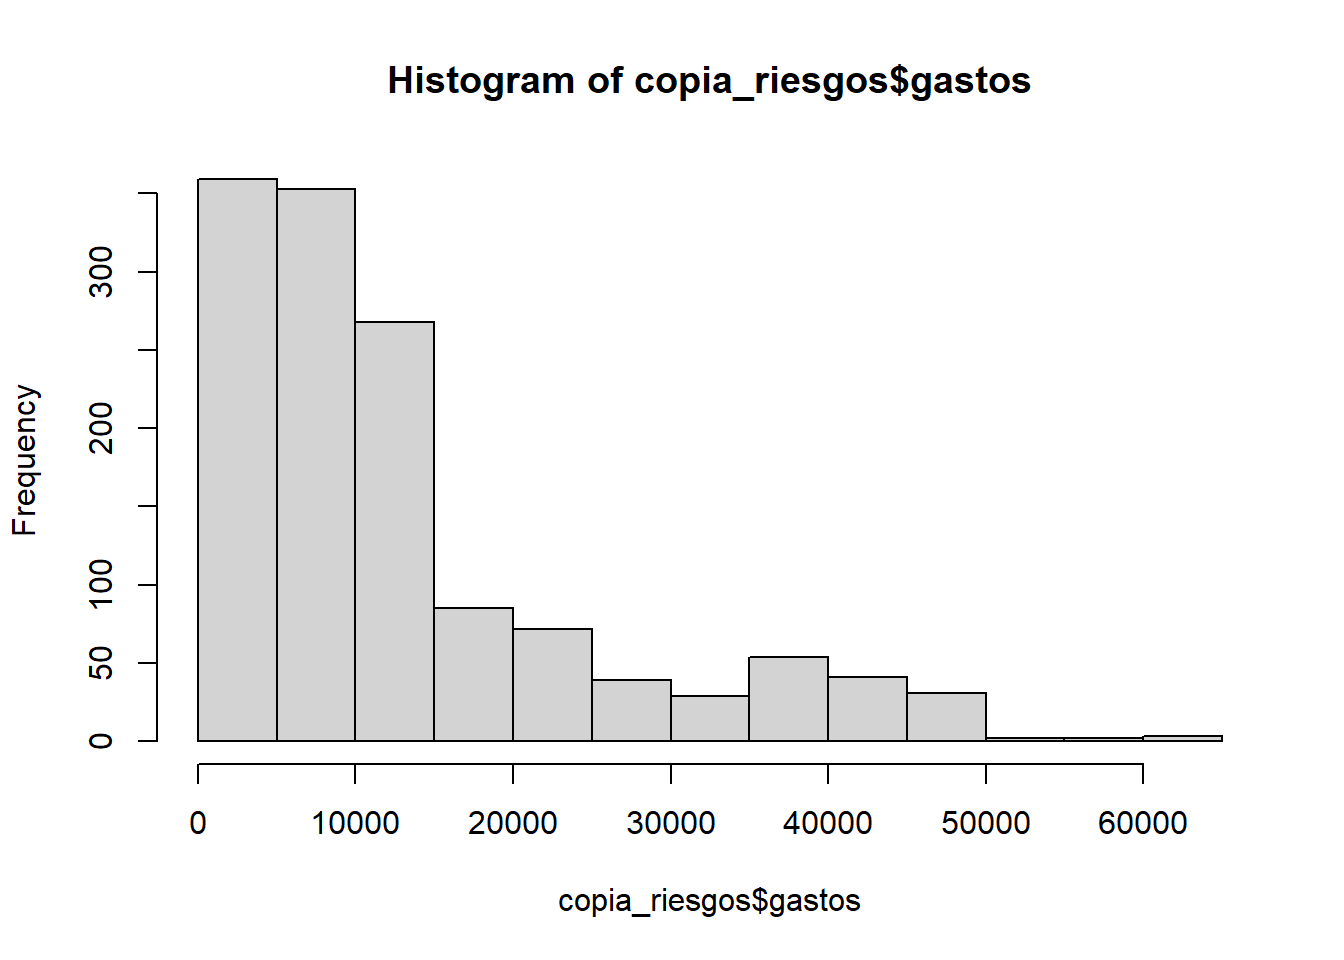
\includegraphics{book_LCC_files/figure-latex/unnamed-chunk-133-1.pdf}

\begin{Shaded}
\begin{Highlighting}[]
\CommentTok{\#A partir del histograma generado se deduce que la mayoria de los asegurados tienen unos gastos por debajo de los 15000€. }
\end{Highlighting}
\end{Shaded}

Obten la matriz de correlación entre los atributos del dataset. ¿Qué atributos parecen estar más y menos relacionados? (cor).

\begin{Shaded}
\begin{Highlighting}[]
\NormalTok{mat\_correlacion }\OtherTok{\textless{}{-}} \FunctionTok{cor}\NormalTok{(copia\_riesgos)}
\NormalTok{mat\_correlacion}
\end{Highlighting}
\end{Shaded}

\begin{verbatim}
##             edad       bmi      hijos     gastos
## edad   1.0000000 0.1092719 0.04246900 0.29900819
## bmi    0.1092719 1.0000000 0.01275890 0.19834097
## hijos  0.0424690 0.0127589 1.00000000 0.06799823
## gastos 0.2990082 0.1983410 0.06799823 1.00000000
\end{verbatim}

\begin{Shaded}
\begin{Highlighting}[]
\CommentTok{\#Según la matriz de correlación entre los atributos generada se podría decir que aquellos que más relacionados están son gastos y edad (0.2990082), y por otro lado, los que menos relacionados están serían hijos y bmi (0.0127589); dejando a un lado las correlaciones con valor 1, que son las correlaciones de los atributos con ellos mismos.}
\end{Highlighting}
\end{Shaded}

Visualiza las relaciones entre los atributos - scatterplot (plot, pairs, pairs.panels).

\begin{Shaded}
\begin{Highlighting}[]
\FunctionTok{ggpairs}\NormalTok{(copia\_riesgos, }\AttributeTok{lower =} \FunctionTok{list}\NormalTok{(}\AttributeTok{continuous =} \StringTok{"smooth"}\NormalTok{), }\AttributeTok{diag =} \FunctionTok{list}\NormalTok{(}\AttributeTok{continuous =} \StringTok{"bar"}\NormalTok{), }\AttributeTok{axisLabels =} \StringTok{"none"}\NormalTok{)}
\end{Highlighting}
\end{Shaded}

\begin{verbatim}
## Warning in check_and_set_ggpairs_defaults("diag", diag, continuous =
## "densityDiag", : Changing diag$continuous from 'bar' to 'barDiag'
\end{verbatim}

\begin{verbatim}
## `stat_bin()` using `bins = 30`. Pick better value with `binwidth`.
## `stat_bin()` using `bins = 30`. Pick better value with `binwidth`.
## `stat_bin()` using `bins = 30`. Pick better value with `binwidth`.
## `stat_bin()` using `bins = 30`. Pick better value with `binwidth`.
\end{verbatim}

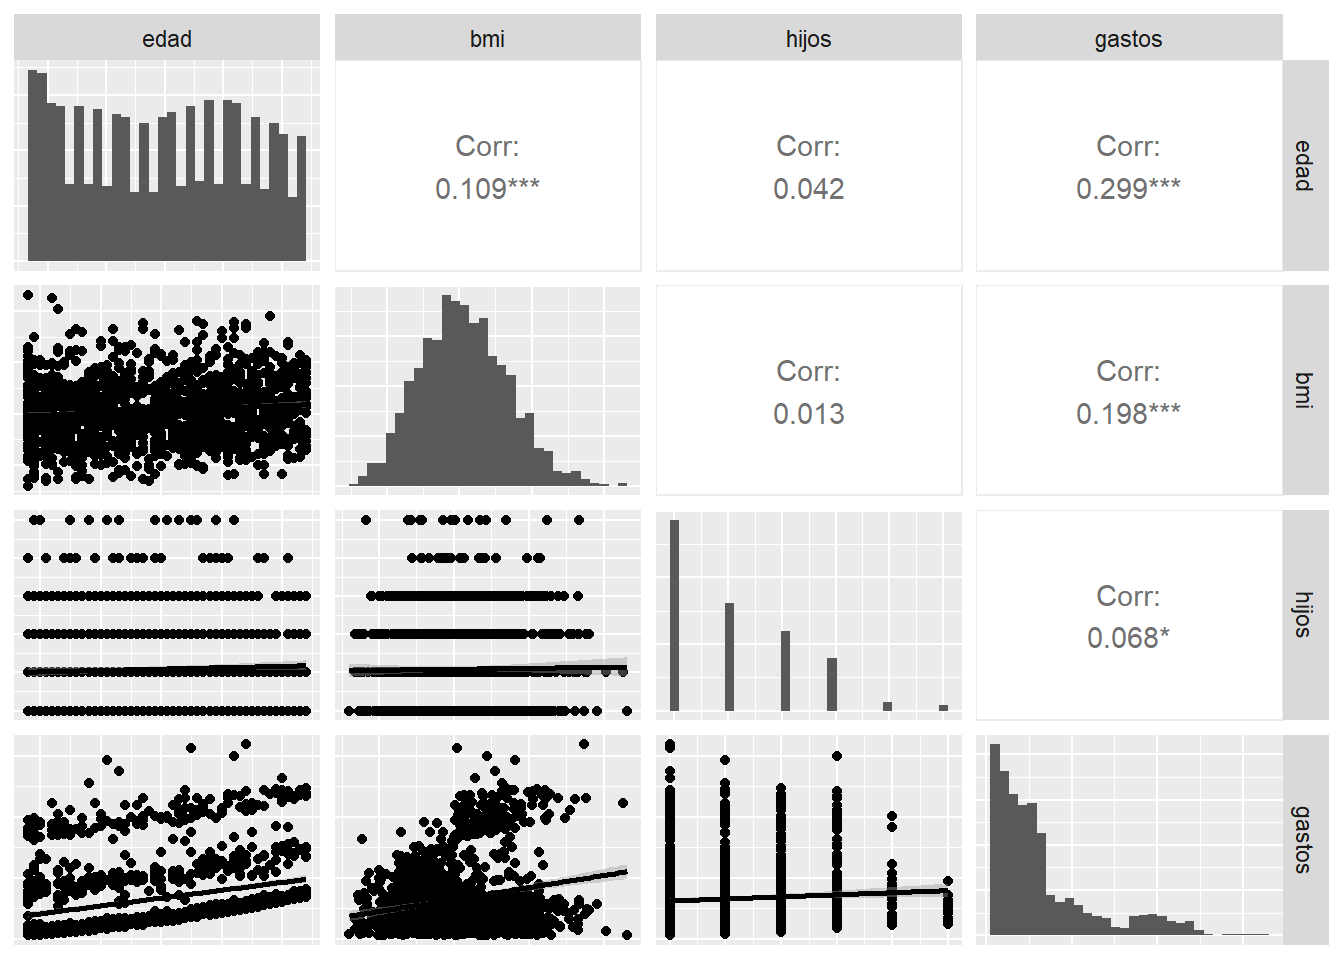
\includegraphics{book_LCC_files/figure-latex/unnamed-chunk-135-1.pdf}

\begin{Shaded}
\begin{Highlighting}[]
\CommentTok{\#Teniendo en cuenta los valores obtenidos en la matriz de correlación anterior, la otra variable que deberia poner en el modelo sería la edad debido a que junto a gastos son las variables con mayor coeficiente de correlación de la matriz. }
\end{Highlighting}
\end{Shaded}

Plantea un modelo lineal m1 de regresión entre gastos y otra variable (la que pienses mejor modela los gastos médicos de los asegurados).

\begin{Shaded}
\begin{Highlighting}[]
\NormalTok{m1 }\OtherTok{\textless{}{-}} \FunctionTok{lm}\NormalTok{(gastos}\SpecialCharTok{\textasciitilde{}}\NormalTok{edad,}\AttributeTok{data=}\NormalTok{copia\_riesgos)}
\NormalTok{m1}
\end{Highlighting}
\end{Shaded}

\begin{verbatim}
## 
## Call:
## lm(formula = gastos ~ edad, data = copia_riesgos)
## 
## Coefficients:
## (Intercept)         edad  
##      3165.9        257.7
\end{verbatim}

\begin{Shaded}
\begin{Highlighting}[]
\FunctionTok{summary}\NormalTok{(m1)}
\end{Highlighting}
\end{Shaded}

\begin{verbatim}
## 
## Call:
## lm(formula = gastos ~ edad, data = copia_riesgos)
## 
## Residuals:
##    Min     1Q Median     3Q    Max 
##  -8059  -6671  -5939   5440  47829 
## 
## Coefficients:
##             Estimate Std. Error t value Pr(>|t|)    
## (Intercept)   3165.9      937.1   3.378 0.000751 ***
## edad           257.7       22.5  11.453  < 2e-16 ***
## ---
## Signif. codes:  0 '***' 0.001 '**' 0.01 '*' 0.05 '.' 0.1 ' ' 1
## 
## Residual standard error: 11560 on 1336 degrees of freedom
## Multiple R-squared:  0.08941,    Adjusted R-squared:  0.08872 
## F-statistic: 131.2 on 1 and 1336 DF,  p-value: < 2.2e-16
\end{verbatim}

\begin{Shaded}
\begin{Highlighting}[]
\CommentTok{\#Con summary hemos obtenido los errores estándar de los coeficientes, los p{-}values, el estadístico F y R cuadrado. El p{-}value  permite determinar si los estimadores de los parámetros son significativamente distintos de 0, es decir, que contribuyen al modelo.}
\CommentTok{\#Tanto la ordenada en el origen como la pendiente son significativas dado que el p{-}value \textless{} 2.2e{-}16. Y el coeficiente de determinación R cuadrado indica que el modelo es capaz de explicar el 8\% de la variabilidad presente en la variable gasto mediante la variable independiente edad. Destacar que cuanto mayor porcentaje del R cuadrado mejor será el modelo.}
\CommentTok{\#Por otro lado, el p{-}value obtenido en el test F (2.2e{-}16) determina que es superior a la varianza explicada por el modelo comparado con la varianza total, por lo que podemos aceptar el modelo como válido y útil.}
\end{Highlighting}
\end{Shaded}

Intenta un modelo m2 usando funciones polinómicas

\begin{Shaded}
\begin{Highlighting}[]
\NormalTok{m2 }\OtherTok{\textless{}{-}} \FunctionTok{lm}\NormalTok{(gastos}\SpecialCharTok{\textasciitilde{}}\NormalTok{edad }\SpecialCharTok{+} \FunctionTok{I}\NormalTok{(gastos}\SpecialCharTok{\^{}}\DecValTok{2}\NormalTok{),}\AttributeTok{data=}\NormalTok{copia\_riesgos)}
\NormalTok{m2}
\end{Highlighting}
\end{Shaded}

\begin{verbatim}
## 
## Call:
## lm(formula = gastos ~ edad + I(gastos^2), data = copia_riesgos)
## 
## Coefficients:
## (Intercept)         edad  I(gastos^2)  
##   2.262e+03    1.174e+02    1.985e-05
\end{verbatim}

\begin{Shaded}
\begin{Highlighting}[]
\FunctionTok{summary}\NormalTok{(m2)}
\end{Highlighting}
\end{Shaded}

\begin{verbatim}
## 
## Call:
## lm(formula = gastos ~ edad + I(gastos^2), data = copia_riesgos)
## 
## Residuals:
##      Min       1Q   Median       3Q      Max 
## -25551.5  -1905.0   -565.5    645.8   8076.5 
## 
## Coefficients:
##              Estimate Std. Error t value Pr(>|t|)    
## (Intercept) 2.262e+03  2.575e+02   8.786   <2e-16 ***
## edad        1.174e+02  6.277e+00  18.709   <2e-16 ***
## I(gastos^2) 1.985e-05  1.551e-07 127.974   <2e-16 ***
## ---
## Signif. codes:  0 '***' 0.001 '**' 0.01 '*' 0.05 '.' 0.1 ' ' 1
## 
## Residual standard error: 3175 on 1335 degrees of freedom
## Multiple R-squared:  0.9314, Adjusted R-squared:  0.9313 
## F-statistic:  9058 on 2 and 1335 DF,  p-value: < 2.2e-16
\end{verbatim}

\begin{Shaded}
\begin{Highlighting}[]
\CommentTok{\#Con summary hemos obtenido los errores estándar de los coeficientes, los p{-}values, el estadístico F y R cuadrado. El p{-}value  permite determinar si los estimadores de los parámetros son significativamente distintos de 0, es decir, que contribuyen al modelo.}
\CommentTok{\#Tanto la ordenada en el origen como la pendiente son significativas dado que el p{-}value \textless{} 2.2e{-}16. Y el coeficiente de determinación R cuadrado indica que el modelo es capaz de explicar el 93\% de la variabilidad presente en la variable gasto mediante la variable independiente edad. Destacar que cuanto mayor porcentaje del R cuadrado mejor será el modelo.}
\CommentTok{\#Por otro lado, el p{-}value obtenido en el test F (2.2e{-}16) determina que es superior a la varianza explicada por el modelo comparado con la varianza total, por lo que podemos aceptar el modelo como válido y útil.}

\CommentTok{\#De hecho el modelo se mejora en un 83\%, lo que es una cifra bastante significativa de mejora}
\end{Highlighting}
\end{Shaded}

\begin{Shaded}
\begin{Highlighting}[]
\NormalTok{m3 }\OtherTok{\textless{}{-}} \FunctionTok{lm}\NormalTok{(gastos}\SpecialCharTok{\textasciitilde{}}\NormalTok{. ,}\AttributeTok{data=}\NormalTok{copia\_riesgos)}
\NormalTok{m3}
\end{Highlighting}
\end{Shaded}

\begin{verbatim}
## 
## Call:
## lm(formula = gastos ~ ., data = copia_riesgos)
## 
## Coefficients:
## (Intercept)         edad          bmi        hijos  
##     -6916.2        240.0        332.1        542.9
\end{verbatim}

\begin{Shaded}
\begin{Highlighting}[]
\FunctionTok{summary}\NormalTok{(m3)}
\end{Highlighting}
\end{Shaded}

\begin{verbatim}
## 
## Call:
## lm(formula = gastos ~ ., data = copia_riesgos)
## 
## Residuals:
##    Min     1Q Median     3Q    Max 
## -13884  -6994  -5092   7125  48627 
## 
## Coefficients:
##             Estimate Std. Error t value Pr(>|t|)    
## (Intercept) -6916.24    1757.48  -3.935 8.74e-05 ***
## edad          239.99      22.29  10.767  < 2e-16 ***
## bmi           332.08      51.31   6.472 1.35e-10 ***
## hijos         542.86     258.24   2.102   0.0357 *  
## ---
## Signif. codes:  0 '***' 0.001 '**' 0.01 '*' 0.05 '.' 0.1 ' ' 1
## 
## Residual standard error: 11370 on 1334 degrees of freedom
## Multiple R-squared:  0.1201, Adjusted R-squared:  0.1181 
## F-statistic: 60.69 on 3 and 1334 DF,  p-value: < 2.2e-16
\end{verbatim}

\begin{Shaded}
\begin{Highlighting}[]
\CommentTok{\#Según los datos extraídos a partir de summary se puede observar que aquellas variables más significativas son aquellas con un p{-}value más cercano a cero, como edad y bmi, los cuales incluso se marcan con tres estrellas que indican que se aproxima mucho a cero. En cuanto a eficiencia, según el R cuadrado obtenido, este modelo es capaz de explicar el 12\% de la variabilidad presente en la variable gastos mediante las variables independientes edad,bmi e hijos, lo cual no es muy bueno que digamos porque para que el modelo fuera bueno este valor debería aproximarse a uno.}
\end{Highlighting}
\end{Shaded}

\begin{Shaded}
\begin{Highlighting}[]
\FunctionTok{anova}\NormalTok{(m1,m2)}
\end{Highlighting}
\end{Shaded}

\begin{verbatim}
## Analysis of Variance Table
## 
## Model 1: gastos ~ edad
## Model 2: gastos ~ edad + I(gastos^2)
##   Res.Df        RSS Df  Sum of Sq     F    Pr(>F)    
## 1   1336 1.7854e+11                                  
## 2   1335 1.3457e+10  1 1.6509e+11 16377 < 2.2e-16 ***
## ---
## Signif. codes:  0 '***' 0.001 '**' 0.01 '*' 0.05 '.' 0.1 ' ' 1
\end{verbatim}

\begin{Shaded}
\begin{Highlighting}[]
\FunctionTok{anova}\NormalTok{(m1,m3)}
\end{Highlighting}
\end{Shaded}

\begin{verbatim}
## Analysis of Variance Table
## 
## Model 1: gastos ~ edad
## Model 2: gastos ~ edad + bmi + hijos
##   Res.Df        RSS Df Sum of Sq      F    Pr(>F)    
## 1   1336 1.7854e+11                                  
## 2   1334 1.7253e+11  2 6.018e+09 23.266 1.169e-10 ***
## ---
## Signif. codes:  0 '***' 0.001 '**' 0.01 '*' 0.05 '.' 0.1 ' ' 1
\end{verbatim}

\begin{Shaded}
\begin{Highlighting}[]
\CommentTok{\#Teniedo en cuenta los resultados que se obtienen al realizar anova con los modelos elaborados anteriormente, sería más interesante estudiar el modelo m2 ya que de los tres modelos es el que presenta un p{-}value más próximo a cero.}
\end{Highlighting}
\end{Shaded}

\hypertarget{text-mining}{%
\chapter{Text Mining}\label{text-mining}}

\hypertarget{text-mining-1}{%
\section{Text Mining 1}\label{text-mining-1}}

\begin{Shaded}
\begin{Highlighting}[]
\FunctionTok{library}\NormalTok{(tm)}
\end{Highlighting}
\end{Shaded}

\begin{verbatim}
## Warning: package 'tm' was built under R version 4.0.5
\end{verbatim}

\begin{verbatim}
## Loading required package: NLP
\end{verbatim}

\begin{verbatim}
## 
## Attaching package: 'NLP'
\end{verbatim}

\begin{verbatim}
## The following object is masked from 'package:ggplot2':
## 
##     annotate
\end{verbatim}

\begin{verbatim}
## 
## Attaching package: 'tm'
\end{verbatim}

\begin{verbatim}
## The following object is masked from 'package:arules':
## 
##     inspect
\end{verbatim}

\begin{Shaded}
\begin{Highlighting}[]
\FunctionTok{library}\NormalTok{(pdftools)}
\end{Highlighting}
\end{Shaded}

\begin{verbatim}
## Warning: package 'pdftools' was built under R version 4.0.5
\end{verbatim}

\begin{verbatim}
## Using poppler version 0.73.0
\end{verbatim}

\begin{Shaded}
\begin{Highlighting}[]
\FunctionTok{library}\NormalTok{(stringr)}
\FunctionTok{library}\NormalTok{(stringi)}
\FunctionTok{library}\NormalTok{(ggplot2)}
\FunctionTok{library}\NormalTok{(RColorBrewer)}
\FunctionTok{library}\NormalTok{(wordcloud)}
\end{Highlighting}
\end{Shaded}

\begin{verbatim}
## Warning: package 'wordcloud' was built under R version 4.0.5
\end{verbatim}

Aplicar Text-Mining a estos pdf's - usando el material visto en clase.

\begin{Shaded}
\begin{Highlighting}[]
\NormalTok{directorio.textos }\OtherTok{\textless{}{-}} \FunctionTok{file.path}\NormalTok{(}\StringTok{"C:"}\NormalTok{, }\StringTok{"pdfstextmining2021"}\NormalTok{)}
\NormalTok{directorio.textos}
\end{Highlighting}
\end{Shaded}

\begin{verbatim}
## [1] "C:/pdfstextmining2021"
\end{verbatim}

\begin{Shaded}
\begin{Highlighting}[]
\FunctionTok{dir}\NormalTok{(directorio.textos)}
\end{Highlighting}
\end{Shaded}

\begin{verbatim}
##  [1] "20200512_conspiracies_covid19.pdf"                                                            
##  [2] "780.2.full.pdf"                                                                               
##  [3] "bmj.n352.full.pdf"                                                                            
##  [4] "ccdrv46i1112a11-eng.pdf"                                                                      
##  [5] "CCE_Briefing_Note_001.pdf"                                                                    
##  [6] "Coronavirus_The_spread_of_misinformation.pdf"                                                 
##  [7] "COVID-19-Mistrust-and-Denial-Factsheet_RCCE-interagency-TWG.pdf"                              
##  [8] "COVID-19_and_The_Rights_of_Persons_with_Disabilities.pdf"                                     
##  [9] "COVID-19_pandemic-_Perception,_confusion_and_consp.pdf"                                       
## [10] "el-mundo-mapfre-110-en.pdf"                                                                   
## [11] "Full_book_FINAL_EN2.0-UNIDO.pdf"                                                              
## [12] "GHSN Policy Report 1.pdf"                                                                     
## [13] "how_to_respond_to_covid-19_deniers.pdf"                                                       
## [14] "ijerph-17-07818.pdf"                                                                          
## [15] "IJHPM38801596396600.pdf"                                                                      
## [16] "Imhoff-Lamberty_COVID-19-Conspiracies_Preprint.v4.pdf"                                        
## [17] "Losers in the crisis_ Europe&#8217;s radical right wing in the COVID-19 pandemic.pdf"         
## [18] "s41590-021-00875-8.pdf"                                                                       
## [19] "socsci-09-00165.pdf"                                                                          
## [20] "Tony Blair Institute, From the Fringes to the Forefront, Far Right Movements and Covid-19.pdf"
## [21] "victims-of-the-pandemic-european-far-right-parties-and-covid-19.pdf"                          
## [22] "Vocal-vaccine-deniers-guidance-document.pdf"
\end{verbatim}

\begin{Shaded}
\begin{Highlighting}[]
\CommentTok{\#Leer los nombres de los ficheros}
\NormalTok{list.files }\OtherTok{\textless{}{-}} \FunctionTok{DirSource}\NormalTok{(directorio.textos)}

\NormalTok{texts }\OtherTok{\textless{}{-}} \FunctionTok{lapply}\NormalTok{(list.files, pdf\_text) }
\end{Highlighting}
\end{Shaded}

\begin{verbatim}
## PDF error: Invalid Font Weight
## PDF error: Invalid Font Weight
## PDF error: Invalid Font Weight
## PDF error: Invalid Font Weight
## PDF error: Invalid Font Weight
## PDF error: Invalid Font Weight
## PDF error: Invalid Font Weight
\end{verbatim}

\begin{Shaded}
\begin{Highlighting}[]
\FunctionTok{length}\NormalTok{(texts)}
\end{Highlighting}
\end{Shaded}

\begin{verbatim}
## [1] 6
\end{verbatim}

\begin{Shaded}
\begin{Highlighting}[]
\NormalTok{texts}
\end{Highlighting}
\end{Shaded}

\begin{verbatim}
## $encoding
## [1] "COVID-19 Conspiracy\r\nTheories: Comparative\r\ntrends in Italy, France,\r\nand Spain\r\nEU DisinfoLab\r\nApril 2020\r\n              EU DisinfoLab –– info@disinfo.eu – www.disinfo.eu\r\n"                                                                                                                                                                                                                                                                                                                                                                                                                                                                                                                                                                                                                                                                                                                                                                                                                                                                                                                                                                                                                                                                                                                                                                                                                                                                                                                                                                                                                                                                                                                                                                                                                                                                                                                                                                                                                                                                                                                                                                                                                                                                                                                                                                                                                                                                                                                                                                                                                                                                                                                                                                                                                                                                                                                                                                                                                                                                                                                                                                                                                                                                                                                                                                                                                                                                                                                                                                                                                                                                                                                                                
## [2] "As the pandemic turns into an infodemic, old and new conspiracy theories find a way to take over\r\nthe public debate. Thanks to our monitoring of independently fact-checked disinformation from\r\nFrance, Italy, and Spain, we have noticed that similar patterns are emerging regarding the types of\r\nconspiracy theories deliberately related to Covid-19. Firstly, we offer a theoretical review of the\r\nindicators and characteristics that define a conspiracy theory, and how the coronavirus fits into\r\nthem. Secondly, the main content and narratives identified at the comparative level are explored\r\nthrough concrete examples in order to map the current conspiracy ecosystem.\r\nDEFINITIONAL CRITERIA AND OPERATIONAL CHARACTERISTICS OF A CONSPIRACY THEORY\r\nConspiracy, from the Latin conspirare – to breathe together – suggests the coming together of\r\nindividuals to obtain a shared outcome (Byford, 2011). The term implies a group of people who make\r\nsecret arrangements to advance their personal interests, consequently causing harm to their\r\ncommunity.\r\nConspiracies rely on the idea of a Manichean struggle between “‘the pure people’ versus ‘the corrupt\r\nelite’” (Mudde, 2004: 543), whether the latter consists of a political, economic or cultural group.\r\nTherefore, a conspiracy theory is first of all a theory of power (Fenster, 1999) and conspiracy\r\ntheorists wish to reverse the power dynamic that oppresses society by awakening or red-pilling their\r\nfellow citizens. Conspiracy theorists attribute the pejorative acceptation of the term to a form of\r\n“stigmatised knowledge” (Barkun, 2016), namely disapproved by mainstream institutions. Looking\r\nat the coronavirus epidemic, conspiracy theories range from entirely fabricated content to the\r\ninstrumentalisation of tentative or speculative findings, to which absolute certainty is attributed, in\r\nwhat resembles a game of Chinese whispers (no pun intended).\r\nHence, conspiracy theories are based on a biased interpretation of reality, which rests on the cherry-\r\npicking of facts to fulfil a certain hypothesis. In some cases, these theories are not falsifiable, but\r\nthe lack of empirical evidence is potentially justified in the eye of the believer, as secrecy is the main\r\ngoal of the clandestine plots they try to unveil. As a result, followers have to take a leap of faith and\r\n‘trust the plan’. While conspiracy theories have always been part of the debate, the prevalence of\r\npersonal beliefs and emotions over hard facts and rational thinking that characterises the era of\r\npost-truth politics has certainly granted them unprecedented legitimacy, as well as the chance to\r\nreach a broader audience.\r\nOverall, conspiracy theories stem from a desire to make sense of a complex world in simplistic\r\nterms, by finding someone to blame for its problematic aspects. A clear enemy provides cognitive\r\ncomfort, whether this exists outside, within or above the targeted community (Walker, 2013).\r\nCoronavirus conspiracies fit all three categories being the result of the evil plan designed by:\r\n     •   A foreign power against other countries (outside),\r\n     •   A malicious minority in the country (within),\r\n     •   The government against its own people (above).\r\nThe next section explores the most recurrent coronavirus-related conspiracy narratives. As we\r\nrecognise that customarily topics come back in a new guise, what Muirhead and Rosenblum (2020)\r\n                                                                                                         2\r\n"
## [3] "called a “conspiracy without theory” is also taking place. This consists of simply pointing out that\r\nsomething is off, while leaving implications to the receiver’s imagination. The screenshot below\r\nshows an image that went viral on social media platforms, representing a train car with COVID-19\r\nwritten on it. Viewers are left to wonder: why is it there? Were the US (where the photo is said to be\r\nfrom) involved, and if so, how?\r\nCONSPIRACY NARRATIVES\r\nThis section now delves into the main narratives of coronavirus-related conspiracy theories\r\nrecurrently encountered in our analysis of European disinformation ecosystems. As anticipated\r\nearlier, most of these arguments are old news (e.g. deepstate scares, anti-Semitism or anti-\r\nvaxxers), which are re-framed under the new Covid-19 guise.\r\nThe three major narratives we identified focus on:\r\n    •    The origins of the virus\r\n    •    The cures and medical treatments for the virus\r\n    •    The instrumental use of the virus to push secret agendas\r\nORIGINS\r\nA great amount of conspiracy theories builds on the idea that the virus is not new, a suspicion that\r\nhas manifested transversely across countries. For instance, disinfection products listing protection\r\nfrom the coronavirus are presented as evidence, disregarding the existence of different CoV viral\r\nstrains.\r\nOrigin-based theories defend the artificial nature of the virus, which spread either accidentally or\r\nintentionally. The accident-centred thread blames without evidence the virus’ spread on the\r\ncarelessness of the actors involved, who conducted covert activities (e.g. a bio-weapon program\r\nwent wrong). Exploitation of resource and consumerism are also pilloried, as some suggest a relation\r\n                                                                                                     3\r\n"                                                                                                                                                                                                                                                                                                                                                                                                                                                                                                                                                                                                                                                                                                                                                                                                                                                                                                                                                                                                                                                                                                                                                                                                                                                                                                                                                                                                                                                                                                                                                                                                                                                                                                                                                                                   
## [4] "of causality between the epidemic and intensive breeding, once again without any scientific\r\nevidence. Similarly, anti-vaxxers link the likelihood of contracting the virus to flu shots.\r\nMultiple Russian sources of disinformation, subsequently echoed in other countries, emphasised the\r\nbacteriological war intent of the pandemic, whether it originated in the United States or China.\r\nAccordingly, the virus was created in a lab and released voluntarily in order to achieve geopolitical\r\n(e.g. a made-up story circulated in Italy that an American veteran was paid to spread the virus to\r\nEurope) or economic gains (e.g. a French research centre was accused on creating the virus in 2004\r\nin order to sell its patented vaccine).\r\nFinally, the 5G conspiracy is almost becoming a narrative of its own, primed in Europe and beyond.\r\nPopular theories are that the coronavirus is transmitted through 5G antennas or that the 5G\r\ntechnology has a negative health impact and thus makes individuals vulnerable to the virus.\r\nCURES AND MEDICAL TREATMENTS\r\nA number of conspiracy theories confuses the long-standing existence of CoV respiratory viruses\r\nwith the new Covid-19, therefore claiming that the cure already exists, and in line with the\r\nabovementioned theory of power, the elite does not want to share it with the whole population. To\r\nillustrate this, Facebook users in France met the news of Prince Charles’ speedy recovery despite\r\nhis old age with suspicion. In Italy (see below), a WhatsApp message listed surviving politicians and\r\nfootball players, suggesting that they might have received a special treatment or immediate cures.\r\nOther dishonest reasons to hide the cure from the masses allegedly include the economic interests\r\ninvolved in selling an overpriced antidote. In France, where the debate on the use of chloroquine is\r\nquite relevant, destabilising transmitters accused the government of refusing patients the\r\n                                                                                                    4\r\n"                                                                                                                                                                                                                                                                                                                                                                                                                                                                                                                                                                                                                                                                                                                                                                                                                                                                                                                                                                                                                                                                                                                                                                                                                                                                                                                                                                                                                                                                                                                                                                              
## [5] "successful cure because the invention of a vaccine would be more profitable, receiving pressure from\r\npharmaceutical companies to do so.\r\nIn addition, coronavirus sceptics refute the mortality of the virus per se. For instance, an Italian\r\npathologist (who has now lost his medical licence) condemned the use of masks and hand sanitisers\r\nfor allegedly preventing our body’s natural defences from naturally defeating the virus.\r\nIn this category we also include Covid-19 deniers, who reject the very existence of the virus,\r\nmaintaining that all victims died of previous pathologies. Recently, the ‘film your hospital’ hashtag\r\nunveiled a worldwide denialist trend. From the United States, to France, Italy and Spain, social media\r\nusers are filming empty hospitals to demonstrate that the virus is a scam. The videos ignore the fact\r\nthat suspected Covid-19 patients are asked to stay away from hospitals and that emergency rooms\r\nhave reduced all non-indispensable contact with the public.\r\nPOLITICAL MANIPULATION OR HOW TO PUSH A SECRET AGENDA\r\nConspiracy theories systematically advocate the existence of secret plots, which the powerful wish\r\nto hide from the public eye, as they entail forms of political manipulation. In the context of the\r\npandemic, we encounter two opposite conspiracies rooted in distrust towards official authorities.\r\nOn the one hand, conspiracy theories denounce that the government is understating the death toll\r\nto keep the population quiet and avoid taking responsibility for the mismanagement. This approach\r\n                                                                                                    5\r\n"                                                                                                                                                                                                                                                                                                                                                                                                                                                                                                                                                                                                                                                                                                                                                                                                                                                                                                                                                                                                                                                                                                                                                                                                                                                                                                                                                                                                                                                                                                                                                                                                                                                                                                                                                                                                                                                                                                                                                                                        
## [6] "received particular attention in Italy, through the diffusion of WhatsApp voice messages from pretend\r\ninsiders: doctors, nurses and doctors’ relatives.\r\nOn the other hand, national authorities are accused of exaggerating the gravity of the situation to\r\ndivert public attention from other problems the country is facing.\r\nA further step in the narrative proposes conspiracy explanations for the government’s reluctance to\r\ncommunicate the ‘real’ situation. Accordingly, the goal is to push an undemocratic and unethical\r\nagenda that would cause public upheavals if known. Population cleansing is a widespread theory\r\nthat emerged in different terms. For instance, China created the virus to solve the overpopulation\r\nproblem, but apparently so did European countries to get rid of the elderly.\r\nConspiracy theorists also fear that the pandemic will be used as an excuse to impose needless mass\r\nvaccinations, whose real purpose is to implement Orwellian mechanisms of social control. To\r\nillustrate this, former tennis player Marat Safin has vocally advocated that the vaccine allegedly\r\ncontains a microchip to subjugate receivers. The theory is not new: almost a decade ago, Taïeb\r\n(2010) wrote about the conspiracy surrounding the national vaccination against the H1N1 virus as\r\npart of a political means of achieving ‘biopower’.\r\nIn addition, conspiracy theorists warn that the lockdown is an excuse to force people in their homes,\r\nwhile authoritarian measures are being implemented, such as the militarisation of Italian cities\r\ncorroborated by decontextualized photos of military tanks, or the execution of NATO exercises in\r\nEurope.\r\nA common goal is to show the collusion of political and economic powers for evil intent. The\r\nscreenshot below, taken from an Italian Telegram group, links the Prime Minister’s choice to appoint\r\nVodafone CEO (Vittorio Colao) as leader of the task force for the reconstruction phase to their\r\ninvolvement in the 5G conspiracy.\r\n                                                                                                    6\r\n"                                                                                                                                                                                                                                                                                                                                                                                                                                                                                                                                                                                                                                                                                                                                                                                                                                                                                                                                                                                                                                                                                                                                                                                                                                                                                                                                                                                                                                                                                                                                 
## [7] "EVERGREEN CONSPIRACIES STEP INTO THE SHOES OF COVID-19\r\nBesides the extensively explored deep-state allegations, other conspiracy theories that do not\r\nentirely fit the previous narratives include:\r\n    •    The prophetic origin of the coronavirus, foreseen by Nostradamus, Bill Gates or The Simpsons.\r\n    •    A revival of anti-Semitism, accusing Jewish communities of spreading the virus for the\r\n         purpose of poisoning the gentiles and sacrificing them as part of religious rituals.\r\nCONCLUDING THOUGHTS\r\nConspiracy theories are based on the idea that a powerful minority is keeping relevant information\r\nfrom the majority of the population.\r\nThese theories aim to make sense of the complexity of reality by finding someone to blame. They are\r\nmanufactured through the biased connection of unrelated events, whose validity is unprovable.\r\nAs the pandemic is a transnational event, so is the driving infodemic, that is to say the same\r\ncoronavirus-related conspiracy theories are diffusing across different countries.\r\nFocusing on current events, we identified three major conspiracy narratives:\r\n     o The man-made origin of the virus, either accidental or intentional.\r\n     o The existence of a cure detained by a small group.\r\n     o The exploitation of the pandemic as a distraction to forward a secret agenda.\r\nLast but not least, the encountered conspiracy theories do not constitute a novelty, ageless\r\nassumptions are simply retrieved and adapted to suit current events.\r\n                                                                                                    7\r\n"                                                                                                                                                                                                                                                                                                                                                                                                                                                                                                                                                                                                                                                                                                                                                                                                                                                                                                                                                                                                                                                                                                                                                                                                                                                                                                                                                                                                                                                                                                                                                                                                                                                                                                                                                                                                                                                                                                                                                                                                                                        
## [8] "EU DisinfoLab –– info@disinfo.eu – www.disinfo.eu"                                                                                                                                                                                                                                                                                                                                                                                                                                                                                                                                                                                                                                                                                                                                                                                                                                                                                                                                                                                                                                                                                                                                                                                                                                                                                                                                                                                                                                                                                                                                                                                                                                                                                                                                                                                                                                                                                                                                                                                                                                                                                                                                                                                                                                                                                                                                                                                                                                                                                                                                                                                                                                                                                                                                                                                                                                                                                                                                                                                                                                                                                                                                                                                                                                                                                                                                                                                                                                                                                                                                                                                                                                                                                          
## 
## $length
## [1] "INS IGHTS\r\n    LET TERS\r\nEdited by Jennifer Sills\r\nRetraction\r\nWe have obtained new evidence, 6 years\r\nafter the publication of our Report\r\n“Ammonia synthesis by N2 and steam elec-\r\ntrolysis in molten hydroxide suspensions\r\nof nanoscale Fe2O3” (1), that there is a trace\r\nNOx– impurity in the nanoscale Fe2O3 that\r\nwas unknown at the time. We no longer\r\nhave the original nanoscale Fe2O3, and\r\nmanufacturers’ content levels of impurities\r\nin chemicals may vary over time. However,\r\nrecently purchased nanoscale Fe2O3 per\r\ngram contains 0.0005 g N as NOx–, and\r\nan 15N2 isotopic tracer analysis conducted\r\nby Wenzhen Li, Yifu Chen, and Hengzhou\r\n                                                                                                                                                                                                                       Downloaded from http://science.sciencemag.org/ on April 29, 2021\r\nLiu at Iowa State University; Shuang Gu at\r\nWichita State University; and author S.L.\r\nsuggests that this trace impurity, rather\r\nthan N2, is the major nitrogen reactant\r\nin the observed ammonia synthesis. We                       when preliminary evidence suggests they          with the public. In the meantime, scientists\r\nare retracting the original Report, and we                  were not a substantial factor (5). To combat     who have the capacity, seniority, and job\r\nencourage exploration of an N2 to NOx–                      this new misinformation, scientists must         security should help value and amplify\r\nintermediate to ammonia pathway, rather                     communicate clearly and dispute inaccu-          the messages and motivations of those\r\nthan direct elemental nitrogen pathway, to                  rate, politically motivated narratives.          who are willing to participate in public\r\nammonia synthesis. All observed stimulation                    Black, Native, and Latinx Americans           engagement, often at the expense of career\r\nof ammonia generation with these (likely                    have shouldered the greatest burden of the       advancement. It is essential for scientists\r\nNOx–-containing) nanoscale Fe2O3 materials,                 unscientific COVID-19 mismanagement              to work across disciplines and integrate\r\nas well as all thermodynamic calculation                    in the United States (6). Protests against       multiple communication strategies to make\r\nresults, remain accurate as documented in                   police brutality have been dismissed as          scientific evidence understandable, engag-\r\nthe original Report.                                        nonurgent or unnecessary, despite evidence       ing, and approachable.\r\nStuart Licht1*, Baochen Cui1, Baohui Wang1, Fang-           that systemic racial injustice disproportion-    Nita Bharti\r\nFang Li1, Jason Lau2, Shuzhi Liu1                           ately kills Black Americans (7). Scientific      Biology Department, Center for Infectious\r\n1\r\n Department of Chemistry, George Washington                                                                  Disease Dynamics, The Pennsylvania State\r\n                                                            evidence, which should be at the forefront       University, University Park, PA 16802, USA.\r\nUniversity, Washington, DC 20502, USA.\r\n2\r\n Department of Chemistry, Contra Costa College,\r\n                                                            of public discussions and policy on health       Email: nita@psu.edu\r\nSan Pablo, CA 94806, USA.                                   and civil rights, has been drowned out by\r\n                                                                                                             RE FERENCES AND NOTES\r\n*Corresponding author. Email: slicht@gwu.edu                political arguments.\r\n                                                                                                              1. B. Deese, R. A. Klain, “Another deadly consequence of\r\n                                                               Scientists cautiously explain uncertainties       climate change: The spread of dangerous diseases,”\r\nREFERENCES AND NOTES\r\n                                                            while politicians and politically motivated          The Washington Post (2017).\r\n    1. S. Licht et al., Science 345, 637 (2014).                                                              2. W. C. Tucker, Ecol. Law Quart. 39, 831 (2012).\r\n                                                            media outlets emphatically cast blame and         3. O. Benecke, S. E. DeYoung, Glob. Pediatr. Health 6,\r\n                                  10.1126/science.abe0412\r\n                                                            misappropriate scientific evidence. Scientists       2333794X19862949 (2019).\r\n                                                            cannot allow propagandists to spread              4. E. Lipton et al., “He could have seen what was coming:\r\n                                                                                                                 Behind Trump’s failure on the virus,” The New York Times\r\nControlling the                                             lies that dismantle a reasoned response\r\n                                                            to COVID-19 or urgently needed progress\r\n                                                                                                                 (2020).\r\n                                                                                                              5. D. M. Dave, A. I. Friedson, K. Matsuzawa, J. J. Sabia, S.\r\n                                                                                                                 Safford, “Black Lives Matter protests, social distancing,\r\ncoronavirus narrative                                       toward health equity and social justice for\r\n                                                            Black Americans. Informed scientists must\r\n                                                                                                                 and COVID-19,” National Bureau of Economic Research\r\n                                                                                                                 Working Paper No. 27408 (2020); https://www.nber.org/\r\nThe corruption of scientific results has                    take a strong public stance on complex               papers/w27408.\r\n                                                                                                              6. “Health equity considerations and racial and ethnic\r\nserious consequences for human health.                      issues, emphasizing evidence to clearly com-         minority groups” (Centers for Disease Control and\r\nClimate change deniers (1, 2) and people                    municate and contextualize scientific results        Prevention, 2020).\r\n                                                                                                              7. L. Peeples, Nature 573, 24 (2019).\r\n                                                                                                                                                                             PHOTO: IRA L. BLACK/CORBIS/GETTY IMAGES\r\nwho amplify anti-vaccine messages (3) have                  to the public, not just to other scientists.\r\n                                                                                                                                           10.1126/science.abd3662\r\ncreated dangerous, enduring myths, giving                   Institutions must recognize that the current\r\nrise to new problems for which scientists                   system of promotion and tenure devalues\r\nmust now find solutions. Now, politicians\r\nare undermining the response to coronavi-\r\n                                                            such communication, at a huge societal cost.\r\n                                                               Irresponsible, unscientific voices have\r\n                                                                                                             Dismantling systemic\r\nrus disease 2019 (COVID-19) by disregarding\r\nscientific facts and the guidance of epidemi-\r\n                                                            killed too many because of their reach\r\n                                                            and efficacy. Academic incentives must be\r\n                                                                                                             racism in science\r\nologists (4). Simultaneously, nonscientists                 updated to meaningfully reward outreach          In his Editorial “Time to look in the mir-\r\nhave asserted that Black Lives Matter                       efforts, and scientific training should          ror” (12 June, p. 1161), H. H. Thorp calls\r\nprotests caused increases in COVID-19 cases,                prepare scientists to discuss their findings     on scientists to recognize systemic racism\r\n780        14 AUGUST 2020 • VOL 369 ISSUE 6505                                                                                           sciencemag.org SCIENCE\r\n                                                                           Published by AAAS\r\n"                                                                                                                                                                                                                                                                                                                                                                                                                                                                                                                                                                                                                                                                                                                                                                                                                                                                                                                                                                                                                                                                                                                                                                                                                                                                                                                                                                                                                                                                                                                                                                                                                                                                                                                                                                                                                                                                                                                                                                                                                                                                                                            
## [2] "                                                  (9). A majority of these leaders claimed to                   4. Petersen et al., MMWR Morb. Mortal. Wkly. Rep. 68,\r\n                                                  be committed to diversity and inclusion, but                     423 (2019).\r\n                                                                                                                5. S. Yaya, BMJ Glob. Health 5, e002913 (2020).\r\n                                                  diversity and inclusion training or programs                  6. Higher Education Statistics Agency, “Who’s working in\r\n                                                  existed in only half of the organizations                        HE?: Personal characteristics”(2019); www.hesa.ac.uk/\r\n                                                  surveyed, and 41% of organizations did not                       data-and-analysis/staff/working-in-he/characteristics.\r\n                                                                                                                   To view the number of Black professors compared with\r\n                                                  monitor diversity (such as employee demo-                        the total number of professors, in the “Personal char-\r\n                                                  graphics) or discrepancies in performance                        acteristics by occupational classification” table, select\r\n                                                  rankings, pay, and promotion (9).                                “Show: Ethnicity” and “Contract levels: Professor.”\r\n                                                                                                                7. N. Rollock, “Staying Power” (University and College\r\n                                                     Unfortunately, scientists from under-                         Union, 2019); www.ucu.org.uk/media/10075/Staying-\r\n                                                  represented groups are often the ones who                        Power/pdf/UCU_Rollock_February_2019.pdf.\r\n                                                  take on the responsibility (often coupled                     8. S. Wood et al., Proc. R. Soc. Ser. B Biol. Sci. 287,\r\n                                                                                                                   20200877 (2020).\r\n                                                  with additional labor and minimal recogni-                    9. Biotechnology Innovation Organization, “Measuring\r\n                                                  tion) of trying to change a racist system                        diversity in the biotech industry: Building an inclusive\r\n                                                  (10). To lighten their burden, white col-                        workforce” (Center for Talent Innovation and BIO,\r\n                                                  leagues should also take responsibility for                      2020); http://go.bio.org/rs/490-EHZ-999/images/\r\n                                                                                                                   Measuring_Diversity_in_the_Biotech_Industry_\r\n                                                  dismantling systemic racism in the science                       Building_an_Inclusive_Workforce.pdf.10.\r\n                                                  community. Although there is no single                       10. M. F. Jimenez et al., Nat. Ecol. Evol. 3, 1030 (2019).\r\n                Preliminary evidence indicates    “one size fits all” approach to addressing\r\n                                                                                                                                              10.1126/science.abd7531\r\n              that protests demanding justice     inequality, there are common themes and\r\n                   for Black Americans, such      actions that can be implemented in scien-\r\n                                                                                                               Untapped resources\r\n                                                                                                                                                                               Downloaded from http://science.sciencemag.org/ on April 29, 2021\r\n               as this one, have not caused a     tific institutions.\r\n                 spike in COVID-19 infections.       Scientists involved in hiring should\r\n                                                  implement advertising strategies, espe-\r\n                                                  cially at leadership levels, that attract\r\n                                                                                                               for medical research\r\n                                                  diverse applicant pools, and they should                     A therapeutic solution to the coronavirus\r\nwithin the science community. As part             facilitate fair decisions by forming diverse                 disease 2019 (COVID-19) pandemic is\r\nof this self-reflection, scientists should        recruitment panels. To retain diverse                        urgently needed, but new drug discovery\r\nconsider the many ways that inequality            individuals, leaders should promote an                       and development are lengthy processes.\r\nmanifests in science, including science’s         inclusive environment. To do so, they must                   Pharmaceuticals derived from plants and\r\nhistorical contributions to discrimina-           develop training material on understand-                     fungi remain important in our armory\r\ntion, the lack of representation in science,      ing and tackling bias and create safe                        against numerous diseases (1, 2), yet much\r\nand the extra burden placed on minority           spaces for professionals to speak freely and                 of plant and fungal biodiversity remains\r\nscientists to fix issues relating to diversity    honestly. All departments should develop                     unexplored for drug discovery (3). Of\r\nand inclusion. Understanding the scope of         zero-tolerance, anti-racism policies and put                 about 350,000 known plant species, 7%\r\nsystemic inequality in science will enable        procedures in place that effectively handle                  have medicinal uses (1, 4), and the wider\r\ngenuine and sustainable efforts to make           complaints about racism and race-related                     potential of the world’s flora to yield new\r\nscientific institutions fair for all.             aggression. Mentoring schemes should be                      medicines has been discussed by conserva-\r\n   Racial categories historically developed       embedded into departments to address the                     tion biologists for decades (5). We urgently\r\nand endorsed by scientists led to a hierar-       neglect that Black, Indigenous, and people                   need a comprehensive scientific study of\r\nchy of groups seen as superior or inferior.       of color often experience when navigating                    biodiversity to inspire, accelerate, and\r\nAlthough unsupported by biological                their career. Underrepresented individuals                   innovate medicinal discovery.\r\nevidence, these categories have had devas-        (many of whom are already used as unpaid                        Acquiring usable plant and fungal\r\ntating effects on non-white communities           consultants) should be given the power to                    material is resource-consuming, but a\r\nthroughout history. The myth that racial          make important decisions.                                    partial solution lies in specimens already\r\ngroups were fundamentally different was              All scientists should recognize the                       housed in herbaria, botanic gardens (6),\r\nused to justify colonialism, slavery, geno-       achievements of diverse individuals.                         and fungal biological resource centers.\r\ncide, and eugenics (1), and it still governs      Recognition includes citing their work,                      Herbaria host about 380 million specimens\r\npolicies today. The intersectionality of rac-     referring them for opportunities, nominat-                   from all described plant species (7), and\r\nism and modern society has left a legacy of       ing them for awards, and teaching their                      botanic gardens maintain about one-third\r\nracial disparities in socioeconomic status        work in classes. Appropriately recognizing                   of all known land plant species (8). Fungal\r\n(2), education (3), and health (4, 5).            the work of underrepresented individu-                       collections currently host about 860,000\r\n   The lack of diversity in scientific institu-   als will enable them (rightly) to be as                      strains worldwide (9). These collections are\r\ntions reveals ongoing systemic racism in the      competitive as their white counterparts                      invaluable resources representing unparal-\r\nfield. As of 2019, less than 1% of UK profes-     when looking to progress professionally. By                  leled chemical diversity.\r\nsors were Black (6). Black female professors      taking these steps, scientists of all back-                     Evolutionary relationships inferred\r\nin the United Kingdom experience bully-           grounds can help create a more inclusive,                    from DNA could be used to guide selec-\r\ning, racial discrimination, and institutional     diverse, and fair community.                                 tion of species with medicinal potential.\r\nneglect (7). Systemic racism has also contrib-                                                                 Just a few milligrams from specimens\r\n                                                  Esther A. Odekunle\r\nuted to the lack of diverse representation.       GlaxoSmithKline, Stevenage, Hertfordshire SG1                enable comprehensive chemical profiling,\r\nEven textbooks currently lack representation      2NY, UK. Email: e.a.odekunle@gmail.com                       uncovering new chemical entities that\r\nof Black female scientists (8). According to                                                                   share chemical or physical characteristics\r\n                                                  REFERENCES AND NOT ES\r\na recent report, leadership positions such                                                                     with drug molecules, potentially with novel\r\n                                                   1. R. J. Cottrol, J. Social Hist. 49, 740 (2015).\r\nas CEO or executive in the biotech industry        2. D. R. Williams et al., Health Psychol. 35, 407 (2016).   modes of action (1). Artificial intelligence\r\nare largely occupied by white professionals        3. K. Weir, Monitor Psychol. 47, 42 (2016).                 and emerging technologies could reveal\r\nSCIENCE sciencemag.org                                                                                               14 AUGUST 2020 • VOL 369 ISSUE 6505              781\r\n                                                                      Published by AAAS\r\n"
## [3] "                                                              INSIG HTS | L E T T E R S\r\n                                                              compounds with mechanistic effects rel-\r\n                                                              evant to diseases threatening humanity (1,\r\n                                                              10). Furthermore, collections are increas-\r\n                 Where\r\n                                                              ingly used to generate genomic data, which\r\n                                                              could be used to identify members of gene\r\n                                                              families known to be involved in the syn-\r\n                Science                                       thesis of useful compounds (11).\r\n                                                                 Investing in a new era of large-scale\r\n                                                              exploration of therapeutic candidates\r\n                 Gets                                         from nature could help humanity prepare\r\n                                                              for future health challenges. Scientists,\r\n                                                              governments, and other stakeholders must\r\n                Social.                                       establish functional and equitable agree-\r\n                                                              ments to ensure that this work complies\r\n                                                              with the Nagoya Protocol and associated\r\n                                                              access and benefit sharing legislation and\r\n                                                              reflects the value and origins of specimens\r\n                                                              collected during the colonial era (12). It is\r\n                                                              also critical that benefits are shared with\r\n                                                              the nations and Indigenous peoples from\r\n                                                              where these resources derive.\r\n                                                                                                                                  Downloaded from http://science.sciencemag.org/ on April 29, 2021\r\n                                                              Oscar A. Pérez-Escobar1, James E. Richardson2,3,\r\n                                                              Melanie-Jayne R. Howes1,4*, Eve Lucas1, Noelia\r\nAAAS.ORG/COMMUNITY                                            Álvarez de Róman5, Jérôme Collemare6, Ian A.\r\n                                                              Graham7, Joachim Gratzfeld5, Paul J. Kersey1, Ilia\r\n                                                              J. Leitch1, Alan Paton1, Peter M. Hollingsworth3,\r\n                                                              Alexandre Antonelli1,8\r\n                                                              1\r\n                                                               Royal Botanic Gardens, Kew, TW9 3AE,\r\n                                                              UK. 2Department of Biology, Faculty of\r\n                                                              Natural Sciences, Universidad del Rosario,\r\n                                                              Bogotá, Colombia. 3Royal Botanic Garden\r\n                                                              Edinburgh, Edinburgh, EH3 5LR, UK. 4Institute\r\n                                                              of Pharmaceutical Science, Faculty of Life\r\n                                                              Sciences & Medicine, King’s College London,\r\n                                                              SE1 9NH, UK. 5Botanic Gardens Conservation\r\n                                                              International, Richmond, TW9 3BW, UK.\r\n                                                              6\r\n                                                                Westerdijk Fungal Biodiversity Institute, Utrecht,\r\n                                                              Netherlands. 7Department of Biology, Centre\r\n                                                              for Novel Agricultural Products, University of\r\n                                                              York, York, YO10 5DD, UK. 8Gothenburg Global\r\n                                                              Biodiversity Centre and University of Gothenburg,\r\n                                                              Gothenburg, Sweden.\r\n                                                              *Corresponding author: Email: m.howes@kew.org\r\n                                                              RE FERENCES AND NOTES\r\nAAAS’ Member Community is a one-stop destination                   1. M.-J. R. Howes et al., Plants, People, Planet. 10.1002/\r\n                                                                      ppp3.10138 (2020).\r\nfor scientists and STEM enthusiasts alike. It’s “Where             2. D. J. Newman, G. M. Cragg, J. Natural Prod. 83, 770\r\n                                                                      (2020).\r\n                                                                   3. J. W. H. Li, J. C. Vederas, Science 325, 161 (2009).\r\n   Science Gets Social”: a community where facts                   4. K. J. Willis, Ed., “State of the World’s Plants 2017”\r\n                                                                      (Royal Botanic Gardens, Kew, UK, 2017); https://\r\n                                                                      stateoftheworldsplants.org.\r\n matter, ideas are big and there’s always a reason to              5. W. F. Laurance et al., Science 278, 1117 (1997).\r\n                                                                   6. E. K. Meineke et al., Ecol. Monographs 88, 505 (2018).\r\n     come hang out, share, discuss and explore.                    7. A. James et al., Appl. Plant. Sci. 6, e1024 (2018).\r\n                                                                   8. R. Mounce et al., Nat. Plants 3, 795 (2017).\r\n                                                                   9. World Data Centre for Microorganisms (WDCM) Culture\r\n                                                                      Collections Information Worldwide (www.wdcm.org/).\r\n                                                                  10. J. M. Stokes et al., Cell 180, 688 (2020).\r\n                                                                  11. R. D. Kersten, J.-K. Wenig, Proc. Natl. Acad. Sci. U.S.A.\r\n                                                                      115, E10961 (2018).\r\n                                                                  12. S. Das, M. Lowe, J. Natural Sci. Collect. 6, 4 (2018).\r\n                                                              COMPETING INTERESTS\r\n                                                              O.A.P.-E. receives financial support from the Swiss\r\n                                                              Orchid Foundation and the Sainsbury Orchid\r\n                                                              Trust. I.A.G. is Director of the United Kingdom\r\n                                                              Research and Innovation–Biotechnology and\r\n                                                              Biological Sciences Research Council (UKRI-\r\n                                                              BBRSC) High Value Biorenewables Network.\r\n                                                              A.A. receives financial support from the Swedish\r\n                                                              Research Council, the Swedish Foundation for\r\n                                                              Strategic Research, the Knut and Alice Wallenberg\r\n                                                              Foundation, and the Royal Botanic Gardens, Kew.\r\n                                                                                                10.1126/science.abc8085\r\n                                                                                              sciencemag.org SCIENCE\r\n                                          Published by AAAS\r\n"                                                                                                                                                                                                                                                                                                                                                                                                                                                                                                                                                                                                                                                                                                                                                                                                                                                                                                                                                                                                                                                                                                                                                                                                                                                                                                                                                                                                                                                                                                                                                                                                                                                                                                                                                                                                                                                                                                                                                                                                                                                                                                                                                                                                                                                                                                                                                                                                                                                                                                                                                                                                                                                                                                                                                                                                                                                                                                                                                                                                                 
## [4] "Controlling the coronavirus narrative\r\nNita Bharti\r\nScience 369 (6505), 780.\r\nDOI: 10.1126/science.abd3662\r\n                                                                                                                        Downloaded from http://science.sciencemag.org/ on April 29, 2021\r\n  ARTICLE TOOLS                   http://science.sciencemag.org/content/369/6505/780.2\r\n  RELATED                         http://stm.sciencemag.org/content/scitransmed/12/557/eabc5332.full\r\n  CONTENT\r\n                                  http://stm.sciencemag.org/content/scitransmed/12/550/eabc3539.full\r\n                                  http://stm.sciencemag.org/content/scitransmed/12/554/eabc1126.full\r\n                                  http://stm.sciencemag.org/content/scitransmed/12/555/eabc9396.full\r\n  REFERENCES                      This article cites 3 articles, 0 of which you can access for free\r\n                                  http://science.sciencemag.org/content/369/6505/780.2#BIBL\r\n  PERMISSIONS                     http://www.sciencemag.org/help/reprints-and-permissions\r\nUse of this article is subject to the Terms of Service\r\nScience (print ISSN 0036-8075; online ISSN 1095-9203) is published by the American Association for the Advancement of\r\nScience, 1200 New York Avenue NW, Washington, DC 20005. The title Science is a registered trademark of AAAS.\r\nCopyright © 2020 The Authors, some rights reserved; exclusive licensee American Association for the Advancement of\r\nScience. No claim to original U.S. Government Works\r\n"                                                                                                                                                                                                                                                                                                                                                                                                                                                                                                                                                                                                                                                                                                                                                                                                                                                                                                                                                                                                                                                                                                                                                                                                                                                                                                                                                                                                                                                                                                                                                                                                                                                                                                                                                                                                                                                                                                                                                                                                                                                                                                                                                                                                                                                                                                                                                                                                                                                                                                                                                                                                                                                                                                                                                                                                                                                                                                                                                                                                                                                                                                                                                                                                                                                                                                                                                                                                                                                                                                                                                                                                                                                                                                                                                                                                                                                                                                                                                                                                                                                                                                                                                                                                                                                                                                                                                                                                                                                                                                                                                                                                                                                                                                                                                                                                                                                                                                                                                                                                                                                                                                                                                                                                                                                                                                                                                                                                                                                                                                                                                                                                                                                                                                                                                                                                                                                                                                                                                                                                                                                                                                                                                                                                                                                                                                                                                                                                                                                                                                                                                                                                                                                                                                                                                                                                                                                                                                                                                                                                                                                                                                                                                                                                                                                                                                                                                                                                                                                                                                                                                                                                                                                                                                                                                                                                                                                                                                                                                                                                                                                                                                                                                                                                                                                                                                                                                                                                                                                                                                                                                                                                                                                                                                                                                                                                                                                                                                                                                                                                                                                                                                                                                                                                                                                                                                                                                                                                                                                                                                                                                                                                                                                                                                                                                                                                                                                                                                                                                                                                                                                                                                                                                                                                                                                                                                                                                                                                                                                                                   
## 
## $position
## [1] "                                                                                                                                  VIEWS AND REVIEWS\r\nBerkshire\r\n                                       ACUTE PERSPECTIVE\r\n                                                                                                                                                                                 BMJ: first published as 10.1136/bmj.n352 on 10 February 2021. Downloaded from http://www.bmj.com/ on 29 April 2021 by guest. Protected by copyright.\r\ndavidoliver372@googlemail.com Follow\r\nDavid on Twitter @mancunianmedic\r\nCite this as: BMJ 2021;372:n352        David Oliver: Mistruths and misunderstandings about covid-19 death\r\nhttp://dx.doi.org/10.1136/bmj.n352\r\nPublished: 10 February 2021            numbers\r\n                                       David Oliver consultant in geriatrics and acute general medicine\r\n                                       I want to set the record straight about some serious        covid-19 still have an initial false negative rate of\r\n                                       misinformation surrounding covid-19 death                   2-29% in people who then go on to test positive or\r\n                                       certification and mortality statistics. I will paraphrase   develop clinical features of covid-19.9\r\n                                       some of the claims that I have heard repeatedly in\r\n                                                                                                   As we know, death certification is a serious\r\n                                       the media:\r\n                                                                                                   professional duty. It is done with diligence and, for\r\n                                       “People are not dying from, but with, covid-19.”            deaths in hospital, is usually discussed with a\r\n                                       “Deaths classified as from covid-19 result from largely     medical examiner (although this step was suspended\r\n                                       false positive polymerase chain reaction (PCR) test         for a few months10 in the first pandemic wave in early\r\n                                       results,” “deaths are mostly from other causes and          2020).\r\n                                       underlying conditions,” “death numbers are grossly\r\n                                                                                                   The personal and professional consequences of\r\n                                       inflated,” “there is no excess mortality compared\r\n                                                                                                   fabricating or distorting certificates would be serious,\r\n                                       with other years or months,” and this is “no different\r\n                                                                                                   and there is no mass conspiracy or incentive,\r\n                                       from a normal flu season.”\r\n                                                                                                   financial or otherwise, to do so. Nor is it credible that\r\n                                       Let’s see, shall we?                                        such a plot would not have been leaked by now via\r\n                                                                                                   disgruntled whistleblowers.\r\n                                       According to the Office for National Statistics (ONS),\r\n                                       the total number of deaths with covid-19 recorded on        We sometimes certify deaths in patients who died\r\n                                       the death certificate in England and Wales has now          from covid-19 or its complications well beyond 28\r\n                                       passed 100 000.1 The government’s daily press               days. A study from Leicester University followed over\r\n                                       releases, however, report “deaths within 28 days of         40 000 people with covid-19 discharged from hospital\r\n                                       a positive test result”—a definition repeated faithfully    for 140 days and found a readmission rate of 31%\r\n                                       by broadcast and print journalists and on social            (23% within 60 days), with 9% dying on\r\n                                       media.2 This approach probably under-recognises             readmission.11 Obviously not all those deaths were\r\n                                       the real number of deaths from covid-19 by around           from covid complications, but it seems clear that\r\n                                       20%.3                                                       many were accelerated by them.\r\n                                       Having two parallel reporting methods is unfortunate        Meanwhile, data are emerging that give the lie to the\r\n                                       as it plays into the “What are they not telling us?”        notion that covid-19 is no worse than or different to\r\n                                       narrative of covid denialists, conspiracy theorists,        seasonal flu. The ONS reported in January 2021 that\r\n                                       and lockdown sceptics.4                                     England and Wales had seen the highest increase in\r\n                                                                                                   excess mortality in 2020 in any year since 1940.12 And\r\n                                       ONS data are based on what doctors responsible for\r\n                                                                                                   a paper in The BMJ comparing 4000 patients with\r\n                                       a patient in their final illness write on the death\r\n                                                                                                   influenza and 12 000 with covid-19 in Wuhan, China,\r\n                                       certificate to the “best of [their] knowledge and\r\n                                                                                                   showed much greater severity of symptoms and much\r\n                                       belief,” and they do not take into account how\r\n                                                                                                   higher morbidity and mortality among those with\r\n                                       recently the deceased had had a positive covid-19 test\r\n                                                                                                   covid-19.13\r\n                                       result.5 I would advise anyone therefore to trust ONS\r\n                                       data above the government’s reporting tool. In 90%          Doctors treating patients with covid-19 over the past\r\n                                       of certificates where covid-19 is recorded, it does so      12 months recognise a very different clinical\r\n                                       in part 1 as the cause contributing directly to death.6     syndrome in the sickest patients and a tide of cases\r\n                                       The Nuffield Trust has issued a similar note of caution     of a kind, severity, and clinical course that we have\r\n                                       about covid-19 death statistics.7                           not seen before. We don’t diagnose cases solely on\r\n                                                                                                   the basis of PCR tests. Furthermore, PCR false positive\r\n                                       In the first few months of the pandemic, access to\r\n                                                                                                   rates are very low in people with symptoms and high\r\n                                       covid-19 testing was scarce even for hospital patients\r\n                                                                                                   pretest probability.7 14\r\n                                       who were clearly infected, let alone for those in care\r\n                                       homes or private residences.8 Some death certificates       Every time we see or hear such mistruths we need to\r\n                                       might therefore have mentioned “covid-19” despite           combat them and call them out. They are used to play\r\n                                       the absence of a positive result if the clinical picture    down the seriousness and consequences of covid-19\r\n                                       was clear. In other cases, doctors might have been          and undermine health protection efforts.\r\n                                       reluctant to put covid-19 on a certificate in the\r\n                                       absence of a test even though the clinical picture was      Competing interests: See bmj.com/about-bmj/freelance-contributors.\r\n                                       clear.\r\n                                                                                                   Provenance and peer review: Commissioned; not externally peer reviewed.\r\n                                       We have far better access to testing now, but\r\n                                       systematic review has shown that PCR tests for\r\nthe bmj | BMJ 2021;372:n352 | doi: 10.1136/bmj.n352                                                                                                                          1\r\n"
## [2] "     VIEWS AND REVIEWS\r\n1     Office for National Statistics. Coronavirus (covid-19) roundup. 2 Feb 2021.\r\n      https://www.ons.gov.uk/peoplepopulationandcommunity/healthandsocialcare/conditionsanddis-\r\n                                                                                                                                                                 BMJ: first published as 10.1136/bmj.n352 on 10 February 2021. Downloaded from http://www.bmj.com/ on 29 April 2021 by guest. Protected by copyright.\r\n      eases/articles/coronaviruscovid19roundup/2020-03-26#:~:text=The%20total%20num-\r\n      ber%20of%20deaths,aged%2075%20years%20and%20over\r\n2     King’s Fund. Deaths from covid-19 (coronavirus). 2020. https://www.kingsfund.org.uk/publica-\r\n      tions/deaths-covid-19\r\n3     Duncan P, Caelainn B. UK official Covid death toll has always undercounted fatalities, analysis\r\n      shows. Guardian 2021 Jan 22. https://www.theguardian.com/world/2021/jan/22/uk-official-covid-\r\n      death-toll-undercounted-fatalities\r\n4     Oliver D. Covid deniers’ precarious Jenga tower is collapsing on contact with reality. BMJ Opinion\r\n      1 Feb 2021. https://blogs.bmj.com/bmj/2021/02/01/david-oliver-covid-deniers-precarious-jenga-\r\n      tower-is-collapsing-on-contact-with-reality/\r\n5     Office for National Statistics, HM Passport Office. Guidance for doctors completing Medical\r\n      Certificates of Cause of Death in England and Wales: for use during the emergency period only.\r\n      2020. https://assets.publishing.service.gov.uk/government/uploads/system/uploads/attach-\r\n      ment_data/file/877302/guidance-for-doctors-completing-medical-certificates-of-cause-of-death-\r\n      covid-19.pdf\r\n6     Spiegelhalter D. The trouble with coronavirus death tolls. Politico 2021 Jan 28.\r\n      https://www.politico.eu/article/coronavirus-deaths-statistics-data-cases-accuracy/.\r\n7     Nuffield Trust. Measuring mortality during covid-19: a Q&A. 14 Jan 2021. https://www.nuffield-\r\n      trust.org.uk/news-item/measuring-mortality-during-covid-19-a-q-a.\r\n8     Health Foundation. NHS test and trace: the journey so far. 2020.\r\n      https://www.health.org.uk/publications/long-reads/nhs-test-and-trace-the-journey-so-far\r\n9     Watson J, Whiting PF, Brush JE. Interpreting a covid-19 test result. BMJ 2020;369:m1808.\r\n      doi: 10.1136/bmj.m1808 pmid: 32398230\r\n10    Oliver D. David Oliver: the medical examiner role could transform our approach to handling death.\r\n      BMJ 2020;370:m3035. doi: 10.1136/bmj.m3035 pmid: 32764076\r\n11    Ayoubkhani D, Khunit K, Nafilyan V, etal. Epidemiology of post-COVID syndrome following\r\n      hospitalisation with coronavirus: a retrospective cohort study.medRxiv 2021. [Preprint.]\r\n      doi: 10.1101/2021.01.15.21249885\r\n12    Covid: 2020 saw most excess deaths since world war two. BBC News 2021 Jan 12.\r\n      https://www.bbc.co.uk/news/uk-55631693\r\n13    Xie Y, Bowe B, Maddukuri G, Al-Aly Z. Comparative evaluation of clinical manifestations and risk\r\n      of death in patients admitted to hospital with covid-19 and seasonal influenza: cohort study. BMJ\r\n      2020;371:m4677. doi: 10.1136/bmj.m4677 pmid: 33323357\r\n14    Kamran A. Covid-19: screening without scrutiny, spending taxpayers’ billions. BMJ\r\n      2020;371:m4487. doi: 10.1136/bmj.m4487\r\n2                                                                                                          the bmj | BMJ 2021;372:n352 | doi: 10.1136/bmj.n352\r\n"                                                                                                                                                                                                                                                                                                                                                                                                                                                                                                                                                                                                                                                                                                                                                                                                                                                                                                                                                                                                                                                                                                                                                                                                                                                                                                                                                                                                                                                                                                                                                                                                                                                                                                                                                                                                                                                                                                                                                                                                                                                                                                                                                                                                                                                                                                                                                                                                                                                                                                                                                                                                                                                                                                                                                                                                                                                                                                                                                                                                                                                                                                                                                                                                                                                                                                                                                                                                                                                                                                                                                                                                                                                                                                                                                                                                                                                                                                                                                                                                                                                                                                                                                                                                                                                                                                                                                                                                                                                                                                                                                                                                                                                                                                                                                                                                                                                                                                                                                                                                                                                                                                                                                                                                                                                                                                                                                                                                                                                                                                                                                                                                                                                                                                                                                                                                                                                                                                                                                                                                                                                                                                                                                                                                                                                                                                                                                                                                                                                                                                                                                                                                                                                                                                                                                                                                         
## 
## $reader
## [1] "             SERIES                                                                                         CANVax - www.canvax.ca\r\nFake news and science denier attacks on\r\nvaccines. What can you do?\r\n  Noni E MacDonald1*\r\n                                                                                                               This work is licensed under a Creative\r\n   Abstract                                                                                                    Commons Attribution 4.0 International\r\n                                                                                                               License.\r\n   Misinformation and disinformation (“fake news”) about vaccines are contagious—travelling\r\n   faster and farther than truth. The consequences are serious; leading to negative impacts on\r\n   health decisions, including vaccine acceptance, and on trust in immunization advice from public             Affiliation\r\n   health and/or healthcare professional. This article provides a brief overview of evidence-based\r\n   strategies to address vaccine deniers in public, in clinical practice and in social situations. As          1\r\n                                                                                                                 Department of Paediatrics,\r\n   well, a strategy to help differentiate between vaccine deniers and simple vaccine refusers in               Dalhousie University, IWK Health\r\n                                                                                                               Centre, Halifax, NS\r\n   a practice or clinic is provided. Five tactics are widely used by vaccine deniers: conspiracy;\r\n   fake experts; selectivity; impossible expectations; and misrepresentation and false logic.\r\n   Recognizing and understanding these tactics can help protect against misinformation and\r\n   science denialism propaganda. Highlighting the strong medical science consensus on the                      *Correspondence:\r\n   safety and effectiveness of vaccines also helps. Carefully and wisely choosing what to say and              noni.macdonald@dal.ca\r\n   speaking up—whether you are at a dinner party, out with friends or in your medical office or\r\n   clinic—is crucial. Not speaking up implies you agree with the misinformation. Having healthcare\r\n   providers recognize and address misinformation using evidence-based strategies is of growing\r\n   importance as the arrival of the coronavirus disease 2019 (COVID-19) vaccines is expected to\r\n   further ramp up the vaccine misinformation and disinformation rhetoric. Healthcare providers\r\n   must prepare themselves and act now to combat the vaccine misinformation tsunami.\r\nSuggested citation: MacDonald NE. Fake news and science denier attacks on vaccines. What can you do? Can\r\nCommun Dis Rep 2020;46(11/12):432–5. https://doi.org/10.14745/ccdr.v46i1112a11\r\nKeywords: science denier, vaccine, misinformation, disinformation\r\nIntroduction                                                             Why does this happen?\r\nNever before has the public been so bombarded by information,            Sadly, we all make most of our decisions based upon our beliefs\r\nnor has it ever been so difficult to know what and whom to               and not upon carefully weighed scientific evidence (6). We see\r\nbelieve. The critical importance of this problem is well illustrated     and hear what we believe, rather than believing what we see\r\nby the World Health Organization (WHO) shining a bright                  and hear (7). We are strongly influenced by what we think others\r\nlight on the coronavirus disease 2019 (COVID-19) pandemic                around us (our social networks) are doing or expecting us to do.\r\ninfodemic (1). Infodemic refers to a rapid and far-reaching spread       We see causation in coincidences and we prefer anecdote and\r\nof both accurate and inaccurate information. Misinformation              stories to data and scientific evidence.\r\n(information that is false but not created with the intention of\r\ncausing harm) and disinformation (or “fake news”; information            The objective of this article is to draw attention to the\r\nthat is false and deliberately created to cause harm) travel faster      importance of fake news and science deniers’ attacks on vaccines\r\nand farther than truth (2,3). Science deniers, including vaccine         in the era of social media. It will describe tactics used by science\r\nscience deniers, have a strong and very effective platform               deniers and highlight strategies healthcare providers can use in\r\nnow—the Web—from which to shill their scientifically-bankrupt            their office or clinic when they encounter a vaccine refuser or a\r\nwares (4). We, who understand the rigor of science and                   science denier as well as providing the URL for a WHO website\r\nknow the evidence supporting immunization for health and                 for report concerning misinformation found online.\r\nwell-being, are often aghast at the falsehoods promulgated\r\nand—too often—accepted and acted upon by members of                      This is the ninth article produced by the Canadian Vaccination\r\nthe public. For example, in the United States, the variation in          Evidence Resource and Exchange Centre (CANVax) in\r\nhuman papillomavirus (HPV) vaccine uptake across the country             the CANVax Briefs series. This centre includes a group of\r\nis better explained by exposure to tweets about HPV than by              multidisciplinary professionals that identify and create useful\r\nsocioeconomic class data (5).                                            resources to foster vaccine uptake (8).\r\nPage 432            CCDR • November 5, 2020 • Vol. 46 No. 11/12\r\n"                                                                                                                                                                                                   
## [2] "CANVax - www.canvax.ca                                                                                               SERIES\r\nWhat can you do?                                                      Highlight scientific consensus\r\n                                                                      Highlighting that there is scientific consensus on the benefits\r\nWhat can you do in the face of this tsunami of misinformation         and value of immunization is also helpful (14) when reacting\r\nand disinformation that is shaping negative beliefs about             to fake news about vaccines and immunization. Share your\r\nimmunization amongst the general public, patients and even,           sources of accurate and quality vaccine information with your\r\noccasionally, among our professional colleagues? Misinformation       patients. These steps will not convince the vocal vaccine denier\r\nis indeed everybody’s problem now (9). The consequences               but are helpful for those who are vaccine hesitant in your target\r\nare serious, leading to negative impacts on health decisions,         audience—your patients and the general public.\r\nincluding vaccine acceptance, and on trust in immunization\r\nadvice from public health and/or healthcare professional. This        Addressing vocal vaccine deniers in public\r\nimpact of misinformation and disinformation will become even          The Regional Office for Europe of WHO has developed effective\r\nmore important when the COVID-19 vaccines arrive, with an             guidance on how to address vocal vaccine deniers in public\r\nexpected further ramp up of vaccine disinformation (10). If           (15,16). This is not an easy task but is an important one to\r\ncounteractions are not taken, the antivaccine movement has the        undertake if the vocal vaccine science denier is having, or has\r\npotential to overwhelm the pro-vaccine voices online (10). You        the potential to have, a significant negative impact on trust in\r\ncan and should help combat this vaccine misinformation tsunami.       immunization in your community.\r\nPrepare yourself: know and recognize tactics                          The WHO guidance is primarily intended for spokespersons of\r\nused by vaccine deniers                                               health authorities who want to prepare themselves for a public\r\n                                                                      event with a vocal vaccine denier, and provides advice on who\r\nKnow the five tactics used widely, often with great vigor, by vocal   should be the spokesperson, dos and don’ts of verbal and non-\r\nvaccine deniers on the Web, in mainstream media and in public         verbal communication, how to behave in a passionate discussion\r\nappearances (11):                                                     and how to protect yourself. It provides helpful and evidence-\r\n•    Conspiracies—drug companies, the government, the health          supported strategies if you should find yourself asked to speak in\r\n     system—pick your scapegoat—are out to trick the general          public.\r\n     public; they withhold information, lie and cover up “the\r\n     truth”                                                           An important point—do not participate in a public discussion if\r\n•    Fake experts—quote or use fake experts and vigorously            you are not media trained.\r\n     denigrate, even decry, real experts\r\n•    Selectivity—refer to obscure and or discredited papers that\r\n     support their argument but omit the vast science that refute     Strategies to address a vaccine science\r\n     it\r\n                                                                      denier in clinical practice\r\n•    Impossible expectations—vaccine must be 100% safe and\r\n     effective—and yet no medical intervention is 100% safe and       Differentiating between a science denier and a\r\n     effective                                                        simple refuser\r\n•    Misrepresentation and false logic—jump to erroneous\r\n     conclusion and use false or illogical analogies                  The first and very important step is to determine if the patient\r\n                                                                      not wanting to take the vaccine is a science denier or a “simple\r\nInterestingly, once you know these tactics they are easy to           refuser”. You may be able to quickly tease this out by asking:\r\nrecognize, as is evidenced by the fake news complaints and the        “What would it take to move you to a “yes” to accept this\r\nmisinformation and disinformation appearing almost daily in the       vaccine?” The simple refuser may pause, think and name the\r\nmainstream and social media.                                          concern. This is even more likely if you have a good rapport and\r\n                                                                      a trusting relationship with the patient. In contrast, you will get\r\nTeach your patients to recognize tactics of                           a very different reaction from the vaccine science denier. They\r\nscience deniers                                                       most often start with a long list of concerns and want to work\r\n                                                                      hard to persuade you to their viewpoint. Beware.\r\nThere are scientific studies that have shown that one way to\r\nprotect the public against fake news and science deniers is to\r\nteach the public about the tactics used, not just correct the\r\nscientific misinformation being presented (12). If an internet site\r\nis the misinformation source, consider reporting it via the WHO\r\nwebsite “How to report misinformation online” (13).\r\n                                                                   CCDR • November 5, 2020 • Vol. 46 No. 11/12                  Page 433\r\n"                                                                                      
## [3] "               SERIES                                                                                       CANVax - www.canvax.ca\r\nStrategies to use when addressing vaccine                               Choose carefully and wisely what to say and speak up—whether\r\nrefusers                                                                it is to a co-worker or a patient or friend. The target audience\r\n                                                                        is not the denier, but those others around you. Remember to\r\nVaccine refusers usually have one or possibly two main concerns.        educate others about disinformation techniques being used and\r\nWhen addressing the concern, heed the following advice:                 help to inoculate against fake news and science denial.\r\n•     Do not make the session a “knowledge dump” as\r\n      overwhelming the refuser with information is rarely helpful       Conclusion\r\n      and may actually end up raising concerns about which the\r\n      refuser was not previously worried                                In light of fake news about vaccines and science deniers’ attacks\r\n•     Do not spend time refuting myths, as this does not change         on vaccines proliferating on both mainstream and social media\r\n      attitudes to immunization (17); furthermore, it may be the        (10), it is critical to learn how to differentiate the real science\r\n      myths that the refuser remembers and not the correct              deniers from vaccine refusers, and how to identify the simple\r\n      information                                                       refusers, who were made unsure in their vaccine acceptance\r\n•     Mini motivational interviewing is a more helpful strategy to      beliefs by the machinations of science deniers. Knowing\r\n      further understand concerns and move the patient towards          and using appropriate strategies for both groups empowers\r\n      acceptance (18,19); WHO has a short conversation guide            healthcare providers to appropriately address situations in\r\n      training module on this technique for immunization that you       professional as well as personal settings.\r\n      might find helpful (20)\r\nStrategies to use when addressing science                               Author’s statement\r\ndeniers\r\n                                                                        NEM—Conceptualization, writing of original draft, reviewing and\r\nThe term “vaccine denier” refers to a member of a subgroup              editing.\r\nat the extreme end of the hesitancy continuum; one who has a\r\nvery negative attitude towards vaccination and is not open to a         Competing interests\r\nchange of mind no matter what the scientific evidence says (11).        NE MacDonald received grants from the Public Health Agency of\r\nThere are several points to remember when addressing science            Canada, the World Health Organization, the Nova Scotia Health\r\ndeniers:                                                                Research Foundation, the Canadian Institutes of Health Research,\r\n•     Do not get into a debate with the denier; it is a time-wasting    the Canadian Immunization Research Network and the Social\r\n      trap                                                              Sciences and Humanities Research Council of Canada. She is a\r\n•     State that science is clearly behind immunization. Again, do      member of the Canadian Vaccination Evidence Resource and\r\n      this without getting into a debate: you are highly unlikely to    Exchange Centre (CANVax) Team.\r\n      convince the denier with your arguments and are likely to\r\n      end up in a unhelpful “yes but” cycle\r\n•     You may try mini motivational interviewing as noted above.\r\n      With strong vaccine science deniers, this is less likely to help\r\n      than with simple refusers, but it is worth a try                  Acknowledgements\r\nLeave the door open                                                     Production of the Canadian Vaccination Evidence Resource\r\nRegardless of whether the patient is a denier or a refuser, if they     and Exchange Centre (CANVax) Briefs has been made possible\r\nchose not to immunize their child or themselves that day, leave         through funding from the Public Health Agency of Canada.\r\nthe door open for future visits and discussion. Do not dismiss          Thank you to the many authors, immunization partners and\r\nthem from your practice—even if that is tempting—as this is not         reviewers who contribute to CANVax.\r\nin the best interests of the patient or the community (21). As well,\r\nit is clinically important to go over the risks and responsibilities if\r\nthe patient chooses not to accept the vaccine(s). The Canadian          Funding\r\nPaediatric Society Caring for Kids website has advice on this that\r\nyou can then retailor to fit your patient’s situation (22).             The development of the Canadian Vaccination Evidence\r\n                                                                        Resource and Exchange Centre Briefs is supported by the\r\nDo not remain silent                                                    Immunization Partnership Funds of the Public Health Agency of\r\nFinally, remember do not remain silent when faced with a vaccine        Canada.\r\nscience denier, as your silence may be interpreted by the others\r\naround you that you are in agreement with the misinformation.\r\nPage 434             CCDR • November 5, 2020 • Vol. 46 No. 11/12\r\n"                                                                                                                                                                                                                                                                                                                                                                                                                                                                
## [4] "CANVax - www.canvax.ca                                                                                           SERIES\r\nReferences                                                         14. van der Linden SL, Clarke CE, Maibach EW. Highlighting\r\n                                                                       consensus among medical scientists increases public support\r\n                                                                       for vaccines: evidence from a randomized experiment. BMC\r\n1.  World Health Organization. Infodemic management -                  Public Health 2015;15:1207. DOI PubMed\r\n    Infodemiology. WHO; 2020 (accessed 2020-10-08).\r\n    https://www.who.int/teams/risk-communication/                  15. World Health Organization Regional Office for Europe. Best\r\n    infodemic-management                                               practice guidance: How to respond to vocal vaccine deniers\r\n                                                                       in public (2017). WHO; 2017 (accessed 2020-10-08).\r\n2.  Bauch CT, Galvani AP. Epidemiology. Social factors in              https://www.euro.who.int/en/health-topics/\r\n    epidemiology. Science 2013;342(6154):47–9. DOI PubMed              disease-prevention/vaccines-and-immunization/\r\n                                                                       publications/2016/best-practice-guidance-how-to-respond\r\n3.  Vosoughi S, Roy D, Aral S. The spread of true and false news       -to-vocal-vaccine-deniers-in-public-2017\r\n    online. Science 2018;359(6380):1146–51. DOI PubMed\r\n                                                                   16. Schmid P, Betsch C. Effective strategies for rebutting\r\n4.  Kata A. Anti-vaccine activists, Web 2.0, and the postmodern        science denialism in public discussions. Nat Hum Behav\r\n    paradigm--an overview of tactics and tropes used online by         2019;3(9):931–9. DOI PubMed\r\n    the anti-vaccination movement. Vaccine 2012;30(25):3778–\r\n    89. DOI PubMed                                                 17. Horne Z, Powell D, Hummel JE, Holyoak KJ. Countering\r\n                                                                       antivaccination attitudes. Proc Natl Acad Sci USA\r\n5.  Dunn AG, Surian D, Leask J, Dey A, Mandl KD, Coiera E.             2015;112(33):10321–4. DOI PubMed\r\n    Mapping information exposure on social media to explain\r\n    differences in HPV vaccine coverage in the United States.      18. Gagneur A, Lemaître T, Gosselin V, Farrands A, Carrier N,\r\n    Vaccine 2017;35(23):3033–40. DOI PubMed                            Petit G, Valiquette L, De Wals P. A postpartum vaccination\r\n                                                                       promotion intervention using motivational interviewing\r\n6.  Kahan DM. Social science. A risky science communication            techniques improves short-term vaccine coverage: PromoVac\r\n    environment for vaccines. Science 2013;342(6154):53–4.             study. BMC Public Health 2018;18(1):811. DOI PubMed\r\n    DOI PubMed\r\n                                                                   19. Gagneur A. Motivational interviewing: A powerful tool\r\n7.  Dubé È, MacDonald NE. Managing the risks of vaccine                to address vaccine hesitancy. Can Commun Dis Rep\r\n    hesitancy and refusals. Lancet Infect Dis 2016;16(5):518–9.        2020;46(4):93–7. DOI PubMed\r\n    DOI PubMed\r\n                                                                   20. World Health Organization. Immunization, Vaccine and\r\n8.  Canadian Public Health Association. The Canadian                   Biologicals. Improving vaccination demand and addressing\r\n    Vaccination Evidence Resource and Exchange Centre.                 hesitancy. WHO (updated 2020-06; accessed 2020-10-08).\r\n    Ottawa (ON): CANVax. https://www.canvax.ca                         http://www.who.int/immunization/programmes_systems/\r\n                                                                       vaccine_hesitancy/en/\r\n9.  Donavan J, Wardle C. Misinformation is Everybody’s\r\n    Problem Now. Social Science Research Council. Items.           21. MacDonald NE, Harmon S, Dube E, Taylor B, Steenbeek\r\n    Insights from the Social Science. SSRC; August 6, 2020             A, Crowcroft N, Graham J. Is physician dismissal of vaccine\r\n    (accessed 2020-10-08). https://items.ssrc.org/covid-               refusers an acceptable practice in Canada? A 2018 overview.\r\n    19-and-the-social-sciences/mediated-crisis/misinformation-i        Paediatr Child Health 2019;24(2):92–7. DOI PubMed\r\n    s-everybodys-problem-now/\r\n                                                                   22. Canadian Paediatric Society. Caring for Kids. When\r\n10. Burki T. The online anti-vaccine movement in the age of            parents choose not to vaccinate: Risks and responsibilities.\r\n    COVID-19. Lancet Digit Health 2020;2(10):e504–5.                   CPS; August 2016 (accessed 2020-10-08). https://www.\r\n    DOI PubMed                                                         caringforkids.cps.ca/handouts/when-parents-choose-no\r\n                                                                       t-to-vaccinate-risks-and-responsibilities\r\n11. Schmid P, MacDonald NE, Habersaat K, Butler R.\r\n    Commentary to: how to respond to vocal vaccine deniers in\r\n    public. Vaccine 2018;36(2):196–8. DOI PubMed\r\n12. van der Linden S, Maibach E, Cook J, Leiserowitz A,\r\n    Lewandowsky S. Inoculating against misinformation. Science\r\n    2017;358(6367):1141–2. DOI PubMed\r\n13. World Health Organization. How to report misinformation\r\n    online. Geneva (Switzerland): WHO; 2020 (accessed\r\n    2020-10-08). https://www.who.int/campaigns/\r\n    connecting-the-world-to-combat-coronavirus/\r\n    how-to-report-misinformation-online\r\n                                                                CCDR • November 5, 2020 • Vol. 46 No. 11/12                Page 435\r\n"
## 
## $mode
##  [1] "          COVID-19\r\n          How hateful\r\n          extremists are\r\n          exploiting the\r\n          pandemic\r\nJuly 2020\r\n"                                                                                                                                                                                                                                                                                                                                                                                                                                                                                                                                                                                                                                                                                                                                                                                                                                                                                                                                                                                                                                                                                                                                                                                                                                                                                                                                                                                                                                                                                                                                                                                                                                                                                                                                                                                                                                                                                                                                                                                                                                                                                                                                                                                                                                                                                                                                                                                                                                                                                                                                                                                                                                                                                                                                                                                                                                                                                                                                                                                                                                                                                                                                                                                                                                                                                                                                                                                                                                                                                                                                                                                                                                                                                                                                                                                                                                                                                                                                                                                                                                                                                                                                                                                                                                                                                                                                                                                                                                                                                                                                                                                                                                                                                                                                                                                                                                                                                                                                                                                                                                                                                                                                                                                                                                                                                                                                                                                                                                                                                                                                                                                                                                                                                                                                                                                                                                                                                                                                                                                                                                                                                                    
##  [2] "Contents\r\n3  Introduction\r\n5  Summary\r\n6  Findings and recommendations\r\n7  Beliefs and attitudes\r\n12 Behaviours and activities\r\n14 Harms\r\n16 Conclusion and recommendations\r\n"                                                                                                                                                                                                                                                                                                                                                                                                                                                                                                                                                                                                                                                                                                                                                                                                                                                                                                                                                                                                                                                                                                                                                                                                                                                                                                                                                                                                                                                                                                                                                                                                                                                                                                                                                                                                                                                                                                                                                                                                                                                                                                                                                                                                                                                                                                                                                                                                                                                                                                                                                                                                                                                                                                                                                                                                                                                                                                                                                                                                                                                                                                                                                                                                                                                                                                                                                                                                                                                                                                                                                                                                                                                                                                                                                                                                                                                                                                                                                                                                                                                                                                                                                                                                                                                                                                                                                                                                                                                                                                                                                                                                                                                                                                                                                                                                                                                                                                                                                                                                                                                                                                                                                                                                                                                                                                                                                                                                                                                                                                                                                                                                                                                                                                                                                                                                                                                                                                                                                                                                                                                 
##  [3] "                                                    Commission for Countering Extremism\r\nIntroduction\r\n                                                                                   that COVID-19 is punishment on China for\r\n                                                                                   their treatment of Uighurs Muslims.3 Other\r\n                                                                                   conspiracy theories suggest the virus is part\r\n                                                                                   of a Jewish plot4 or that 5G is to blame.5 The\r\n                                                                                   latter has led to attacks on 5G masts and\r\n                                                                                   telecoms engineers.6 We are seeing many of\r\n                                                                                   these same narratives reoccur across a wide\r\n                                                                                   range of different ideologies.\r\n                                                                                   Fake news about minority communities has\r\n                                                                                   circulated on social media in an attempt to\r\n                                                                                   whip up hatred. These include false claims\r\n                                                                                   that mosques have remained open during\r\nSince the outbreak of the coronavirus (COVID-19)                                   lockdown.7 Evidence has also shown that\r\npandemic, the Commission for Countering                                            ‘Far Right politicians and news agencies [...]\r\nExtremism has heard increasing reports of                                          capitalis[ed] on the virus to push forward their\r\nextremists exploiting the crisis to sow division                                   anti-immigrant and populist message’.8 Content\r\nand undermine the social fabric of our country.                                    such as this normalises Far Right attitudes and\r\n                                                                                   helps to reinforce intolerant and hateful views\r\nWe have heard reports of British Far Right                                         towards ethnic, racial or religious communities.\r\nactivists and Neo-Nazi groups promoting\r\nanti-minority narratives by encouraging users                                      Practitioners have told us how some Islamist\r\nto deliberately infect groups, including Jewish                                    activists may be exploiting legitimate concerns\r\ncommunities1 and of Islamists propagating                                          regarding securitisation to deliberately drive a\r\nanti-democratic and anti-Western narratives,                                       wedge between communities and the British\r\nclaiming that COVID-19 is divine punishment                                        state.9 Others told us about the difficulties\r\nfrom Allah on the West for their alleged                                           of delivering vital counter-extremism work\r\n‘degeneracy’.2 Islamists have also claimed                                         during lockdown.10 They told us how assessing\r\n1\r\n   Nikita Malik. 2020. ‘Self-Isolation Might Stop Coronavirus, but It Will Speed the Spread of Extremism’, Foreign Policy, (accessed: 8 June 2020), <https://\r\n   foreignpolicy.com/2020/03/26/self-isolation-might-stop-coronavirus-but-spread-extremism/>\r\n2\r\n   Tony Blair Institute for Global Change. 2020. ‘Snapshot: How Extremist Groups are Responding to Covid-19’, p.3, (accessed: 11 June 2020), <https://\r\n   institute.global/sites/default/files/2020-05/Snapshot%203%20COVID19%20V02.pdf>\r\n3\r\n   Nur Aziemah Azman. 2020. ‘‘Divine Retribution’: The Islamic State’s COVID-19 Propaganda’, The Diplomat, (accessed: 8 June 2020), <https://thediplomat.\r\n   com/2020/03/divine-retribution-the-islamic-states-covid-19-propaganda/>\r\n4\r\n   Community Security Trust. 2020. ‘Coronavirus and the plague of Antisemitism’, p.5, (accessed: 08 June 2020), <https://cst.org.uk/data/file/d/9/\r\n   Coronavirus%20and%20the%20plague%20of%20antisemitism.1586276450.pdf>\r\n5\r\n   Aidan Milan. 2020. ‘Coronavirus UK: Why do people think 5G is responsible for the Covid-19 pandemic?’, Metro, (accessed: 8 June 2020), <https://metro.\r\n   co.uk/2020/04/02/coronavirus-uk-people-think-5g-responsible-covid-19-pandemic-12500019/>\r\n6\r\n   Alex Hern. 2020. ‘5G conspiracy theories fuel attacks on telecoms workers’, The Guardian, (accessed: 11 June 2020), <https://www.theguardian.com/\r\n   business/2020/may/07/5g-conspiracy-theories-attacks-telecoms-covid>\r\n7\r\n   See: Community Security Trust. 2020. ‘Coronavirus and the plague of Antisemitism’ p.9, (accessed: 1 June 2020), <https://cst.org.uk/data/file/d/9/\r\n   Coronavirus%20and%20the%20plague%20of%20antisemitism.1586276450.pdf> and Lizzie Dearden. 2020. ‘Coronavirus: Government issues\r\n   disinformation warning as extremists and conspiracy theorists exploit crisis’, The Independent, (accessed: 11 June 2020), <https://www.independent.\r\n   co.uk/news/uk/home-news/coronavirus-conspiracy-theory-warning-disinformation-uk-government-a9429101.html>\r\n8\r\n   Ofra Klein. 2020. ‘How is the Far-Right Capitalising on COVID-19’, Centre for Analysis of the Radical Right, (accessed: 24 June 2020), <http://www.\r\n   radicalrightanalysis.com/2020/04/10/how-is-the-far-right-capitalizing-covid-19/>\r\n9\r\n   CCE Meeting with practitioners 1 June 2020\r\n10\r\n   CCE Meeting with practitioners 3 June 2020\r\n                                                                                3\r\n"
##  [4] "                                              Commission for Countering Extremism\r\nthe scale and impact of extremist content and\r\n                                                                              Our summary of hateful extremism is:\r\ndeveloping counter-extremism interventions\r\nhas become challenging now that extremists                                    • Behaviours that can incite and amplify\r\noperate predominantly online.                                                   hate, or engage in persistent hatred, or\r\n                                                                                equivocate about and make the moral\r\nMany organisations are doing important                                          case for violence;\r\nwork to understand the relationship between\r\nthe COVID-19 pandemic and extremism. By                                       • And that draw on hateful, hostile or\r\nbringing existing information together and                                      supremacist beliefs directed at an\r\ncommissioning original research, these notes                                    out-group who are perceived as a threat\r\nseek to provide an overview of some of the                                      to the wellbeing, survival or success of\r\nattitudes, beliefs and extremist activities                                     an in-group;\r\nthat are taking place across England and                                      • And that cause, or are likely to cause\r\nWales. It represents the first of a series of                                   harm to individuals, communities or\r\nquarterly notes which will collate and analyse                                  wider society.\r\nthis information to help practitioners, civil\r\nsociety and policy makers understand the\r\ncurrent and emerging picture around hateful                                The data collection period for this note is\r\nextremism and work towards developing a                                    1 March to 5 June 2020. The data used in\r\nmore effective response.                                                   this note is publicly available, but we have\r\n                                                                           also included information directly sourced\r\n                                                                           from practitioners who are working in local\r\n Methodology                                                               communities across the country. The data\r\nThe independent Commission for Countering                                  collected in this note is not an exhaustive\r\nExtremism was established in March 2018                                    list of extremist activity but seeks to provide\r\nto support society to challenge all forms of                               an overview. There is limited data available\r\nextremism and provide impartial advice to                                  to assess the scale and harm of extremist\r\nthe Government on new policies. In October                                 activity and we continue to encourage the\r\n2019 we published the report, Challenging                                  Government to develop a strategy that seeks\r\nHateful Extremism.                                                         to address this.\r\nWe are presenting the data according to                                    As this note is the first in the series, we\r\nthe three key pillars of hateful extremism                                 welcome feedback on what might be helpful\r\nidentified in that report:                                                 to include in subsequent versions.11\r\n• Beliefs and attitudes                                                    In addition to this we hope to include original\r\n                                                                           research to identify hateful extremist\r\n• Behaviours and activity\r\n                                                                           narratives in our next note.\r\n• Harms\r\n11\r\n   Please email info@extremismcommission.indepedent.gov.uk to provide feedback\r\n                                                                         4\r\n"                                                                                                                                                                                                                                                                                                                                                                                                                                                                                                                                                                                                                                                                                                                                                                                                                                                                                                                                                                                                                                                                                                                                                                                                                                                                                                                                                                                                                                                                                                                                                                                                                                                                                                                                                                          
##  [5] "                                                     Commission for Countering Extremism\r\nSummary\r\n12 13 14 15 16 17\r\n    37% 21%\r\n                                                          There was a\r\n     of respondents had heard\r\n       about the 5G conspiracy\r\n           theory and almost a                                                                                             A fake post\r\n        third of (those) people                          increase in hate                                         accusing Muslims of\r\n            found it credible12\r\n                                                            crime toward                                            breaking lockdown\r\n                                                           East Asian and                                             rules was shared\r\n       It was reported that\r\n               circa      50                            South East Asian                                         2,700 times                             14\r\n      masts were targeted\r\n                                                              individuals13\r\n              for arson and\r\n       vandalism in the UK\r\n                                                                   90.6%\r\n                  in April16\r\n            Far Right actors                                                                                                    of posts\r\n             have sought to                             containing misinformation were not acted\r\n  encourage other online                                              on by social media companies\r\n      users to deliberately                                         after volunteers flagged them15\r\n                infect Jews\r\n             and Muslims17\r\n12\r\n   Patrik Hermansson. 2020. ‘Trust no one: Understanding the drivers of conspiracy theory belief’, HOPE not hate, p.5, (accessed: 8 June 2020), <https://\r\n   www.hopenothate.org.uk/wp-content/uploads/2020/04/conspiracy-report-2020-04-v1-copy.pdf>\r\n13\r\n   Jamie Grierson. 2020. ‘Anti-Asian hate crimes up 21% in UK during coronavirus crisis’, The Guardian, (accessed: 8 June 2020), <https://www.theguardian.\r\n   com/world/2020/may/13/anti-asian-hate-crimes-up-21-in-uk-during-coronavirus-crisis>\r\n14\r\n   Reuters. 2020. ‘False claim: British mosque remains open during coronavirus lockdown’, (accessed: 8 June 2020), <https://www.reuters.com/article/uk-\r\n   factcheck-leeds-mosque/false-claimbritish-mosque-remains-openduring-coronavirus-lockdown-idUSKBN21I3AX>\r\n15\r\n   \aCenter for Countering Digital Hate. 2020. ‘#Will to Act: How social media giants have failed to live up to their claims on the Coronavirus ‘infodemic’’, p.9,\r\n    (accessed: 8 June 2020), <https://252f2edd-1c8b-49f5-9bb2-cb57bb47e4ba.filesusr.com/ugd/f4d9b9_17e9f74e84414524bbe9a5b45afdf77e.pdf>\r\n16\r\n    Isobel Asher Hamilton. 2020. ‘Here’s what we know about the bizarre coronavirus 5G conspiracy theory that is leading people to set cellphone masts on\r\n    fire’, Business Insider, (accessed: 8 June 2020), <https://www.businessinsider.com/coronavirus-conspiracy-5g-masts-fire-2020-4?r=US&IR=T#some-50-\r\n    masts-have-now-been-targeted-by-arson-attacks-despite-appeals-from-the-government-and-mobile-companies-14>\r\n17\r\n     Rakib Ehsan. 2020. ‘Weaponising COVID-19: Far-Right Antisemitism in the United Kingdom and United States’, Henry Jackson Society, p.13, (accessed:\r\n    11 June 2020), <https://henryjacksonsociety.org/wp-content/uploads/2020/05/HJS-COVID-19-Far-Right-Report.pdf>\r\n                                                                               5\r\n"                                                                                                                                                                                                                                                                                                                                                                                                                                                                                                                                                                                                                                                                                                                                                                                                                                                                                                                                                                                                                                                                                                                                                                                                                                                                                                                                                                                                                                                                                                                                                                                                                                                                                                                                                                                                                                                                                                                                                                                                                                                                                                                                                                                                                                                                                                                                                                  
##  [6] "                                Commission for Countering Extremism\r\nFindings and\r\nrecommendations\r\n Findings                                            • An assessment of how extremism\r\n                                                       manifests locally, the harm it causes, the\r\n • During the COVID-19 pandemic we have                scale of support for extremist narratives\r\n   seen an increased visibility of conspiracy          and how best to pre-empt extremist\r\n   theories ranging from anti-vaccine,                 activity. This should also include a\r\n   anti-establishment to anti-minority and             mechanism to provide bespoke support\r\n   antisemitic. They are not specific to any           to local authorities most affected.\r\n   one ideology, but are used by the Far\r\n                                                     • An assessment of who is most susceptible\r\n   Right, Far Left and Islamists to further\r\n                                                       to extremist narratives and a plan of what\r\n   their own ideological aims.\r\n                                                       interventions they will put in place to\r\n • Hateful extremists have used the                    engage and support those people.\r\n   pandemic to engage in disinformation              • Plans to work with researchers\r\n   and fake news about minority groups                 and practitioners to build a better\r\n   which have been used by sympathisers                understanding of ‘what works’ in relation\r\n   to incite hatred, justify violence and to           to counter extremism online and offline.\r\n   divide communities.\r\n                                                     • A commitment to ensure hateful\r\n • The scale of extremist content online is            extremism falls within the remit of the\r\n   vast. De-platforming Far Right actors               new online harms regulator and that\r\n   has pushed many onto fringe platforms               existing laws on inciting hatred should\r\n   such as Telegram, VK and GAB.                       be enforceable online.\r\n • The short and long term impacts of                • Plans to build an understanding of\r\n   the pandemic could create conditions                how conspiracy theories contribute\r\n   conducive for extremism. Extremists will            to extremism. Including how they\r\n   seek to capitalise on the socio-economic            are utilised by extremists, what the\r\n   impacts of COVID-19 to cause further long           scale, impact and harm is, and how\r\n   term instability, fear and division in Britain.     to counter them. This should include\r\n                                                       a commitment to develop a system to\r\n                                                       classify dangerous conspiracy theories\r\n Recommendations                                       based on the harm they cause.\r\n Government needs to include clear plans             • Separately, the Ministry of Housing,\r\n to counter extremism in their response                Communities and Local Government\r\n to this and future crises. It should also             must drive forward a COVID-19\r\n publish a new counter-extremism strategy              cohesion strategy to help bring different\r\n urgently to ensure that it can strategically          communities together to prevent\r\n respond to the activities of extremists in            extremist narratives from having\r\n our country. This strategy should include:            significant reach and influence.\r\n                                                   6\r\n"                                                                                                                                                                                                                                                                                                                                                                                                                                                                                                                                                                                                                                                                                                                                                                                                                                                                                                                                                                                                                                                                                                                                                                                                                                                                                                                                                                                                                                                                                                                                                                                                                                                                                                                                                                                                                                                                                                                                                                                                                                                                                                                                                                                                                                                                                                                                                                                              
##  [7] "                                                    Commission for Countering Extremism\r\nBeliefs and attitudes\r\nWe have looked at several polls and identified                                   During the COVID-19 pandemic we have\r\nthree themes we consider to be relevant to                                       seen an increased visibility of conspiracy\r\nhateful extremism:                                                               theories ranging from anti-vaccine,\r\n                                                                                 anti-establishment to anti-minority and\r\n• conspiracy theories                                                            antisemitic. They are not specific to any\r\n                                                                                 one ideology, but are used by the Far Right,\r\n• blaming the ‘other’ and out-groups\r\n                                                                                 Far Left and Islamists to further their own\r\n• pro-social attitudes and resilience                                            ideological aims.\r\nThe evidence gathered in this section seeks                                      • Whilst many conspiracy theories may be\r\nto highlight changes in attitudes during this                                       considered harmless, some have resulted\r\nperiod and concerning trends.                                                       in very real-world consequences. The\r\n                                                                                    conspiracy theory that claimed ‘faster\r\n                                                                                    5G internet [was] either causing or\r\nConspiracy theories                                                                 accelerating the spread of the coronavirus’\r\nConspiracy theories have been a key tactic                                          gained significant traction.20 We know that\r\nused by extremists to recruit and divide                                            extremists discussed this theory on fringe\r\ncommunities. Conspiracy theories are                                                social media platforms such as Telegram.\r\ndefined as ‘attempts to explain the ultimate                                        It was reported that circa 50 5G masts were\r\ncauses of significant social and political                                          targeted for arson and vandalism in the UK\r\nevents and circumstances with claims                                                in April.21\r\nof secret plots by two or more powerful\r\n                                                                                 • Although now largely debunked, 5G\r\nactors’.18 They are difficult to challenge as\r\n                                                                                    conspiracy theories permeated rapidly\r\ntheir proponents commonly respond to\r\n                                                                                    into the mainstream. Studies showed that\r\nattempts to invalidate them by claiming\r\n                                                                                    37% of respondents had heard about the\r\nthat they are being censored. Moreover,\r\n                                                                                    5G conspiracy theory and almost a third of\r\nsocial media companies can serve to fuel\r\n                                                                                    (those) people found it credible.22\r\nconspiracy theories as platforms can be slow\r\nto takedown content and some algorithms\r\ncan push users towards more similar\r\nextremist content.19\r\n18\r\n   Karen M. Douglas, Joseph E. Uscinski, Robbie M. Sutton, Aleksandra Chichocka, Turkay Nefes, Chee Siang Ang and Ferzani Deravi. 2019. ‘Understanding\r\n   Conspiracy Theories’, Advances in Political Psychology, Vol. 40:S1, p.4\r\n19\r\n   Adam Smith. 2020. ‘Facebook knew its algorithm made people turn against each other but stopped research’, The Independent, (accessed: 10 June 2020),\r\n   <https://www.independent.co.uk/life-style/gadgets-and-tech/news/facebook-algorithm-bias-right-wing-feed-a9536396.html>\r\n20\r\n   Isobel Asher Hamilton. 2020. ‘Here’s what we know about the bizarre coronavirus 5G conspiracy theory that is leading people to set cellphone masts on\r\n   fire’, Business Insider, (accessed: 8 June 2020), <https://www.businessinsider.com/coronavirus-conspiracy-5g-masts-fire-2020-4?r=US&IR=T>\r\n21\r\n   Isobel Asher Hamilton. 2020. ‘Here’s what we know about the bizarre coronavirus 5G conspiracy theory that is leading people to set cellphone masts on\r\n   fire’, Business Insider, (accessed: 8 June 2020), <https://www.businessinsider.com/coronavirus-conspiracy-5g-masts-fire-2020-4?r=US&IR=T#some-50-\r\n   masts-have-now-been-targeted-by-arson-attacks-despite-appeals-from-the-government-and-mobile-companies-14>\r\n22\r\n    Patrik Hermansson. 2020. ‘Trust no one: Understanding the drivers of conspiracy theory belief’, HOPE not hate, p.5, (accessed: 8 June 2020), <https://\r\n   www.hopenothate.org.uk/wp-content/uploads/2020/04/conspiracy-report-2020-04-v1-copy.pdf>\r\n                                                                              7\r\n"                                                                                                                                                                                                                                                                                                                                                                                                                                                                                                                                                                                                                 
##  [8] "                                                     Commission for Countering Extremism\r\n• People’s beliefs about the causes of the                                          • Despite the scale of conspiracy theories\r\n       pandemic are influencing their behaviour.                                        online, social media companies are not\r\n       Another analysis found that those who                                            doing enough to tackle this problem. The\r\n       believed that COVID-19 was created in a                                          Center for Countering Digital Hate looked\r\n       lab were over twice as likely to have met                                        at misinformation online and showed that\r\n       up with friends during lockdown, and to                                          only 9% of the posts flagged to companies\r\n       believe ‘too much fuss is being made about                                       were met with meaningful action.27\r\n       coronavirus’.23                                                                  This study demonstrates that despite\r\n                                                                                        efforts from social media companies,\r\n• A study from the University of Oxford\r\n                                                                                        harmful content is still spreading on\r\n       found that people who held coronavirus\r\n                                                                                        their platforms.\r\n       conspiracy beliefs were less likely to\r\n       comply with social distancing guidelines\r\n       or take up future vaccines. They tested\r\n       conspiracy theories which claimed that\r\n       the virus is a bioweapon developed by\r\n       China to destroy the West; that Muslims\r\n       are spreading the virus as an attack on\r\n       Western values and that Bill Gates created\r\n       the virus to reduce the world population.24\r\n• The scale of online extremist content and\r\n       engagement with such material is deeply\r\n       concerning. Research by the Institute for\r\n       Strategic Dialogue (ISD) found hundreds\r\n       of thousands of Far Right posts around                                       Blaming the ‘other’ or out-groups\r\n       COVID-19 and millions of engagements\r\n       with known disinformation sites.25 They                                      As we showed in our report and in line\r\n       found that there was a marked increase                                       with social movement theory,28 extremists\r\n       in conversations within Far Right circles                                    promote hostile and supremacist beliefs\r\n       about ‘elites’ such as Bill Gates, George                                    towards a group of people who are perceived\r\n       Soros, the Rothchilds and Jeff Bezos and                                     as a threat to the wellbeing, survival or\r\n       false information about their role in the                                    success of a defined ‘in-group’. Who is seen\r\n       creation of the virus.26                                                     as the ‘out-group’ depends on the ideological\r\n                                                                                    worldview of extremists, but it often includes\r\n23\r\n   \a obby Duffy, Daniel Allington, Kelly Beaver, Christoph Meyer et al. 2020. ‘Life under lockdown: Coronavirus in the UK’, The Policy Institute, King’s College\r\n   B\r\n      London, (accessed: 8 June 2020), <https://www.kcl.ac.uk/policy-institute/assets/coronavirus-in-the-uk.pdf>\r\n24\r\n   \aUniversity of Oxford. 2020. ‘Conspiracy beliefs reduce the following of government coronavirus advice’, (accessed: 8 June 2020), <http://www.ox.ac.uk/\r\n      news/2020-05-22-conspiracy-beliefs-reduces-following-government-coronavirus-guidance>\r\n25\r\n    Study focused predominantly on the US\a\r\n26\r\n    \aInstitute for Strategic Dialogue. 2020. ‘COVID-19 Disinformation Briefing No.3’, (accessed 8 June 2020), <https://www.isdglobal.org/isd-publications/\r\n      covid-19-disinformation-briefing-no-3/>\a\r\n27\r\n     \aCenter for Countering Digital Hate. 2020. ‘#Will to Act: How social media giants have failed to live up to their claims on the Coronavirus ‘infodemic’’, p.3,\r\n      (accessed: 8 June 2020), <https://252f2edd-1c8b-49f5-9bb2-cb57bb47e4ba.filesusr.com/ugd/f4d9b9_17e9f74e84414524bbe9a5b45afdf77e.pdf>\r\n28\r\n      J.M. Berger. 2018. Extremism, London: MIT Press\r\n                                                                                 8\r\n"                                                                                                                                                                                                                                                                                                                                                                                                                                                                                                                                                                                                                                                                                                                                                                                                                                                                                                                                                                                                                                                                                                                                                                                                                                                                                                      
##  [9] "                                                    Commission for Countering Extremism\r\npeople with a protected characteristic, or                                         are that the virus is fake and part of a\r\npeople who possess different racial, ethnic,                                       Jewish plot to mislead the public, that\r\nreligious or cultural backgrounds which are                                        it’s real and was deliberately created for\r\nthen perceived to be ‘alien’ and a threat.29                                       malevolent purposes, that Jews are the\r\n                                                                                   primary spreaders of the virus, that Jewish\r\nHateful extremists often look for someone to                                       people are dying in disproportionately\r\nblame in times of crisis and we have heard                                         higher numbers and posts that incite\r\nhow disinformation and fake news targeted                                          others to deliberately spread the virus to\r\nat different ‘out-groups’ and minorities can                                       Jews.32 Research has shown how similar\r\nbe used to incite hatred, justify violence and                                     antisemitic narratives can gain traction\r\ndivide communities.                                                                within the UK and the US.33\r\nAnti-Western                                                                   • Research has shown how individuals\r\n                                                                                   such as David Icke play a significant\r\n• Islamist extremists have used the                                                role in spreading antisemitic conspiracy\r\n    COVID-19 pandemic to pursue their own                                          theories linked to COVID-19. One of Icke’s\r\n    ideological agendas and objectives. ISIS                                       most popular videos claimed that ‘the\r\n    celebrated the impact of COVID-19 on                                           Rothchilds’ are key players in a global\r\n    Western militaries in the Middle East and                                      plot to use the disease as a pretence to\r\n    sub-Saharan Africa.30 Analysis of their                                        impose a totalitarian world government.\r\n    weekly newsletter showed that ISIS see the                                     This video was viewed over 5.9 million\r\n    pandemic as beneficial to their terrorist                                      times.34 Although Icke was successfully\r\n    aims as defence and security resources                                         de-platformed from Youtube and\r\n    in Western countries are reallocated to                                        Facebook35, the scale and reach of his\r\n    combat the pandemic.31                                                         antisemitic conspiracy theories remains\r\n                                                                                   extremely concerning.\r\nAntisemitism                                                                   Anti-Muslim hatred\r\n• Since the outbreak of the COVID-19                                           • In an attempt to whip up anti-Muslim\r\n    pandemic, five dangerous categories of                                         hatred, fake news and false narratives\r\n    conspiracy theories aimed at blaming                                           showing British Muslims flouting social\r\n    the Jewish community emerged. These                                            distancing rules were promoted. In one\r\n29\r\n    J.M. Berger. 2018. Extremism, London: MIT Press\r\n30\r\n   Tony Blair Institute for Global Change. 2020. ‘Snapshot: How Extremist Groups are Responding to Covid-19’, p.3, (accessed: 8 June 2020), <https://\r\n   institute.global/sites/default/files/2020-05/Snapshot%203%20COVID19%20V02.pdf>\r\n31\r\n   Tony Blair Institute for Global Change. 2020. ‘Snapshot: How Extremist Groups are Responding to Covid-19’, p.3, (accessed: 8 June 2020), <https://\r\n   institute.global/sites/default/files/2020-05/Snapshot%203%20COVID19%20V02.pdf>\r\n32\r\n   Community Security Trust. 2020. ‘Coronavirus and the plague of Antisemitism’, (accessed: 8 June 2020), <https://cst.org.uk/data/file/d/9/Coronavirus%20\r\n   and%20the%20plague%20of%20antisemitism.1586276450.pdf\r\n33\r\n   Rakib Ehsan. 2020. ‘Weaponising COVID-19: Far-Right Antisemitism in the United Kingdom and United States’, Henry Jackson Society, (accessed: 12 June\r\n   2020), <https://henryjacksonsociety.org/wp-content/uploads/2020/05/HJS-COVID-19-Far-Right-Report.pdf>\r\n34\r\n   Center for Countering Digital Hate. 2020. ‘#DeplatformIcke: How Big Tech powers and profits from David Icke’s lies and hate, and why it must stop’, p.4,\r\n   (accessed: 23 June 2020), <https://252f2edd-1c8b-49f5-9bb2-cb57bb47e4ba.filesusr.com/ugd/f4d9b9_db8ff469f6914534ac02309bb488f948.pdf>\r\n35\r\n   Hope Not hate. 2020. ‘Coronavirus & the Far Right: Weekly Round Up’, (accessed: 23 June 2020), <https://www.hopenothate.org.uk/2020/05/07/covid-19-\r\n   the-far-right-weekly-round-up-6/>\r\n                                                                             9\r\n"                                                                                                                                                                                                                                                                                                                                                                                                                                                                                                                                                                                           
## [10] "                                                    Commission for Countering Extremism\r\n    particular case a picture taken outside                                        Pro-social and resilience\r\n    of a Leeds mosque appeared to show\r\n    Muslims breaking the rules. Although                                           Pro-social attitudes can reduce the impact\r\n    quickly refuted by West Yorkshire police,                                      of extremist narratives. In contrast, research\r\n    and shown to be false, it had already gained                                   indicates that a ‘lack of trust in the system\r\n    traction on social media.36 Reports showed                                     is generally higher amongst those who are\r\n    that it was shared 2,700 times on Facebook                                     most prone to believing conspiracy theories’.41\r\n    and was subsequently removed.37\r\n                                                                                   At the start of lockdown, many polls\r\n• Whilst there is no evidence that Muslims                                         suggested that pro-social attitudes were\r\n    have been less assiduous about social                                          higher than normal, indicating that people\r\n    distancing than other communities,                                             felt that the UK Government’s handling of the\r\n    research also showed that 20% of                                               pandemic was better than other countries.\r\n    respondents had read or seen articles\r\n    relating to ‘British Muslims keeping                                           • On 14 April Kekst reported that people in\r\n    mosques open in contravention of the                                              the UK were more likely to have gained\r\n    Government’s lockdown rules’.38                                                   confidence in their government, key\r\n                                                                                      institutions and businesses compared with\r\n• An account purporting to be Far Right\r\n                                                                                      people in the US, Germany, or Sweden.42\r\n    actor Stephen Yaxley-Lennon shared posts\r\n    that branded infected Muslims as ‘corona                                       • In April King’s College London found that\r\n    bombs’ to his followers on Telegram, using                                        there was near-universal support (89%) for\r\n    #GermJihad.39                                                                     the current measures, and 68% strongly\r\n                                                                                      agreed with them.43\r\nAnti-Chinese hatred\r\n• There has also been a worrying rise in hate                                      Whilst support for the Government at the\r\n    crime and hate incidents towards Chinese                                       beginning of the outbreak remained strong,\r\n    people. L1ght, an AI-based start-up that                                       this did not remain the case for long.\r\n    detects and filters toxic online content,\r\n    reported that there was a 900% increase                                        At the peak infection rate on 27 March,\r\n    in hashtags identified as hateful towards                                      YouGov reported that 72% of the public\r\n    Chinese people on Twitter.40                                                   believed the Government was handling the\r\n36\r\n   Professor Imran Awan and Roxana Khan-Williams. 2020. ‘Coronavirus, fear and how Islamophobia Spreads on social media’, p.5, (accessed: 8 June\r\n   2020), <https://antimuslimhatredworkinggrouphome.files.wordpress.com/2020/04/research-briefing-report-7-1.pdf>\r\n37\r\n   Reuters. 2020. ‘False claim: British mosque remains open during coronavirus lockdown’, (accessed: 8 June 2020), <https://www.reuters.com/article/uk-\r\n   factcheck-leeds-mosque/false-claimbritish-mosque-remains-openduring-coronavirus-lockdown-idUSKBN21I3AX>\r\n38\r\n   Patrik Hermansson. 2020. ‘Trust no one: Understanding the drivers of conspiracy theory belief’, HOPE not hate, p.16, (accessed: 8 June 2020) <https://\r\n   www.hopenothate.org.uk/wp-content/uploads/2020/04/conspiracy-report-2020-04-v1-copy.pdf>\r\n39\r\n   Center for Countering Digital Hate. 2020. ‘British far-right adopts Indian hate campaign blaming Muslims for coronavirus’, (accessed: 23 June 2020),\r\n   <https://www.counterhate.co.uk/post/british-far-right-adopts-indian-hate-campaign-blaming-muslims-for-coronavirus>\r\n40\r\n   L1ght. 2020. ‘Rising Levels of Hate Speech & Online Toxicity During This Time of Crisis’, (accessed: 8 June 2020), <https://l1ght.com/Toxicity_during_\r\n   coronavirus_Report-L1ght.pdf?fbclid=IwAR12yPh-GIi1Ur1qwwZoCuu4nP2zG5dLxs590Exli5UXYORQCWp3w_ko1MQ>\r\n41\r\n   Patrik Hermansson. 2020. ‘Trust no one: Understanding the drivers of conspiracy theory belief’, HOPE not hate, p.5, (accessed: 8 June 2020), <https://\r\n   www.hopenothate.org.uk/wp-content/uploads/2020/04/conspiracy-report-2020-04-v1-copy.pdf>\r\n42\r\n   Kekst. 2020. ‘COVID-19 Opinion Tracker’, (accessed 8 June 2020), <https://www.kekstcnc.com/media/2568/kekst-report-16apr2020.pdf>\r\n43\r\n   Bobby Duffy, Daniel Allington, Kelly Beaver, Christoph Meyer et al. 2020. ‘Life under lockdown: Coronavirus in the UK’, The Policy Institute, King’s College\r\n   London, (accessed: 8 June 2020), <https://www.kcl.ac.uk/policy-institute/assets/coronavirus-in-the-uk.pdf>\r\n                                                                               10\r\n"                                                                                                                                                                                                 
## [11] "                                                    Commission for Countering Extremism\r\nissue of COVID-19 ‘very’ or ‘somewhat’ well.\r\nNine weeks later, on 29 May, this dropped to\r\n41% indicating that the public is rapidly losing\r\ntrust in the Government.44\r\nA reduction of trust in the Government\r\nand state institutions can be exploited by\r\nextremists to spread their hateful and\r\ndivisive narratives.\r\nDespite pessimism towards the Government,\r\nresearch showed that more people believed\r\nthat Britain will be more united and kinder\r\nfollowing the recovery from the coronavirus\r\npandemic, than it was before the pandemic.45\r\n44\r\n   YouGov. 2020. ‘YouGov COVID-19 tracker: government handling’, (accessed: 8 June 2020), <https://yougov.co.uk/topics/international/articles-\r\n   reports/2020/03/17/perception-government-handling-covid-19>\r\n45\r\n   Office for National Statistics. 2020. Coronavirus and the social impacts on Great Britain: 14 May 2020, (accessed: 30 June 2020), <https://www.ons.gov.uk/\r\n   peoplepopulationandcommunity/healthandsocialcare/healthandwellbeing/bulletins/coronavirusandthesocialimpactsongreatbritain/14may2020#underst\r\n   anding-the-impact-on-society>\r\n                                                                              11\r\n"                                                                                                                                                                                                                                                                                                                                                                                                                                                                                                                                                                                                                                                                                                                                                                                                                                                                                                                                                                                                                                                                                                                                                                                                                                                                                                                                                                                                                                                                                                                                                                                                                                                                                                                                                                                                                                                                                                                                                                                                                                                                                                                                                                                                                                                                                                                                                                                                                                                                                                                                                                                                                                                                                                                                                                                                                                                                                                                                                                                                                                                                                                                                                                                                                                                                                                                                                                                                                                                                                                                                                                                                                                                                                                                                                                                                                                                                                                                                                                                                                                                                                                                                                                                                                                                                                                                                                                                                                                                                                                                                                                                                                                                                                                                                                                                                                                                                                   
## [12] "                                                    Commission for Countering Extremism\r\nBehaviours and\r\nactivities\r\nWe have seen a range of concerning                                                     An account purporting to be well known\r\nbehaviours across the ideological                                                      Far Right actor, Stephen Yaxley-Lennon,\r\nspectrum of extremism.                                                                 has amassed circa 36,000 followers\r\n                                                                                       on Telegram.51\r\nFar Right                                                                         • A Telegram account purporting to be Jayda\r\n                                                                                       Fransen, former deputy leader of Britain\r\n• The British National Socialist Movement,46\r\n                                                                                       First, was seen promoting conspiracy\r\n    encouraged other Telegram users who\r\n                                                                                       theories about Bill Gates and China on her\r\n    had COVID-19 to deliberately infect Jews\r\n                                                                                       Telegram channel to circa 2,000 followers.\r\n    and Muslims.47\r\n• ISD found that the COVID-19 pandemic\r\n    is playing into ‘accelerationism’ on the\r\n    extreme right. Accelerationism promotes\r\n    the idea that democracy is a failure and\r\n    that Far Right groups should accelerate\r\n    its end through inciting social conflict\r\n    and violence.48\r\n• Social Media platform TikTok banned\r\n    Far Right actors Stephen Yaxley-Lennon\r\n    (Tommy Robinson) and Britain First for\r\n    hate speech violations in April, however\r\n    their combined videos had already\r\n    amassed almost a million views.49 De-\r\n    platforming has pushed many Far Right\r\n    actors and groups onto fringe platforms\r\n    such as Telegram, VK and GAB.50\r\n46\r\n   The British National Socialist Movement is a group that espouses Neo-Nazi views, including comments about Hitler. See: Rakib Ehsan. 2020.\r\n   ‘Weaponising COVID-19: Far-Right Antisemitism in the United Kingdom and United States’, Henry Jackson Society, p.9, (accessed: 11 June 2020),\r\n   <https://henryjacksonsociety.org/wp-content/uploads/2020/05/HJS-COVID-19-Far-Right-Report.pdf>\r\n47\r\n   Rakib Ehsan. 2020. ‘Weaponising COVID-19: Far-Right Antisemitism in the United Kingdom and United States’, Henry Jackson Society, p.13, (accessed: 11\r\n   June 2020), <https://henryjacksonsociety.org/wp-content/uploads/2020/05/HJS-COVID-19-Far-Right-Report.pdf>\r\n48\r\n   Institute for Strategic Dialogue. 2020. ‘COVID-19 Disinformation Briefing No.1’, p.2, (accessed: 8 June 2020), <https://www.isdglobal.org/wp-content/\r\n   uploads/2020/03/COVID-19-Briefing-Institute-for-Strategic-Dialogue-27th-March-2020.pdf>\r\n49\r\n   Tony Blair Institute for Global Change. 2020. ‘How extremist groups are responding to COVID-19’, p.8, (accessed: 8 June 2020), <https://institute.global/\r\n   sites/default/files/2020-05/Snapshot%203%20COVID19%20V02.pdf>\r\n50\r\n   Telegram describes itself as ‘a messaging app with a focus on speed and security’. VK is a Russian online social media and social networking service\r\n   with offices based in Saint Petersburg. VK is available in multiple languages but it is predominantly used by Russian-speakers. GAB describes itself\r\n   as, ‘A social network that champions free speech, individual liberty and the free flow of information online’. See: Ryan Greer. 2020. ‘Weighing the Value\r\n   and Risks of Deplatforming’ Global Network on Extremism & Terrorism, (accessed: 11 June 2020), <https://gnet-research.org/2020/05/11/weighing-\r\n   the-value-and-risks-of-deplatforming/?utm_source=Tech+Against+Terrorism&utm_campaign=1235ee09e6-EMAIL_CAMPAIGN_2019_03_24_07_51_\r\n   COPY_01&utm_medium=email&utm_term=0_cb464fdb7d-1235ee09e6-141624359>\r\n51\r\n   As of 8 June 2020\r\n                                                                              12\r\n"                                                                                                                                                                                                                                                                                                                                                                                                                                                                                                                                                                                                                                                                                                                                                                                                                                                                                                                                                                                                                                                                                                                                                                                                                                                                                                                                                                                                                                                                                                                                                                                                                                                                                                                                                                                                                              
## [13] "                                                     Commission for Countering Extremism\r\n• In the UK, users of multiple Far Right                                           • Practitioners told us how some Islamist\r\n    Telegram channels, attempted to organise                                           activists may be exploiting legitimate\r\n    a lockdown protest. One announced a                                                concerns regarding securitisation\r\n    ‘March against a vaccine and lockdown’ in                                          to further drive a wedge between\r\n    May.52 On Saturday 16 May we saw a small                                           communities and the Government. This\r\n    protest against the lockdown in London,                                            has taken the form of conspiracy theories\r\n    similar to those seen in the US.53 People                                          on social media accusing the Government\r\n    attended for many different reasons,                                               of attempting to use future vaccines to\r\n    however media reports seemed to suggest                                            deliberately harm minority communities\r\n    protestors were generally distrustful of                                           and that COVID-19 is a conspiracy used to\r\n    Government and the media.                                                          control the population.56\r\n                                                                                   • Some memes are used by groups to\r\nIslamist                                                                               further their ideological aims. The image\r\n                                                                                       to the left uses the phrase ‘Sheeple’ which\r\n• In the UK, Islamist extremist group Hizb ut-\r\n                                                                                       is a popular phrase amongst Far Right\r\n    Tahrir54 have used the COVID-19 pandemic\r\n                                                                                       actors and was featured on the US website\r\n    to further their anti-democratic narratives\r\n                                                                                       Infowars. It is a contraction of ‘sheep’ and\r\n    by calling for the establishment of the\r\n                                                                                       ‘people’. In this context it refers to people\r\n    Khilafah (Caliphate) as ‘both a political and\r\n                                                                                       who are easily led and docile. The image\r\n    theological necessity for which no sacrifice\r\n                                                                                       itself references many conspiracy theories\r\n    is too small’.55\r\n                                                                                       such as that the Government and/or an\r\n                                                                                       elite is planning to use COVID-19 to justify\r\n                                                                                       planting tracking chips in people. Although\r\n                                                                                       popular with the Far Right, it has also\r\n                                                                                       circulated amongst other communities.\r\n                                                                                   Going forward we expect to see an increase\r\n                                                                                   in anti-Government conspiracy theories,\r\n                                                                                   particularly pushing the narrative of the\r\n                                                                                   deliberate securitisation of particular\r\n                                                                                   communities. We have already seen\r\n                                                                                   these themes emerge across the\r\n                                                                                   ideological spectrum.\r\n52\r\n   Hope Not hate. 2020. ‘Coronavirus & the Far Right: Weekly Round Up’, (accessed: 8 June 2020), <https://www.hopenothate.org.uk/2020/04/24/covid-19-\r\n   the-far-right-weekly-round-up-4/>\r\n53\r\n   Lizzie Dearden. 2020. ‘Coronavirus: Inside the UK’s biggest anti-lockdown protest’, The Independent, (accessed: 8 June 2020), <https://www.independent.\r\n   co.uk/news/uk/home-news/coronavirus-lockdown-protests-uk-london-hyde-park-5g-conspiracy-theories-a9518506.html>; BBC. 2020. ‘Coronavirus\r\n   lockdown protest: What’s behind the US demonstrations’, (accessed: 8 June 2020), <https://www.bbc.co.uk/news/world-us-canada-52359100>\r\n54\r\n   An organisation that seeks to establish a theocratic Islamic state\r\n55\r\n   Editor. 2020. ‘COVID-19: Is this the end of Liberalism’, Hizb UT-Tahrir, (accessed: 8 June 2020), <http://www.hizb.org.uk/viewpoint/covid-19-is-this-the-\r\n   end-of-liberalism/>\r\n56\r\n   CCE meeting with practitioners, 1 June 2020\r\n                                                                                13\r\n"                                                                                                                                                                                                                                                                                                                                                                                                                                              
## [14] "                                                   Commission for Countering Extremism\r\nHarms\r\nOur report identified six categories of harm                                       In our report, we highlighted that a crucial\r\nfrom extremism which is having an impact                                           element to building resilience to extremism\r\nacross the whole of society. These include:                                        in young people is the provision of youth\r\n                                                                                   services. We highlighted the negative\r\n• social division and intolerance                                                  effect of funding cuts and the related\r\n                                                                                   increases in the risk of young people\r\n• crime, violence and harassment\r\n                                                                                   becoming involved in anti-social activity and\r\n• mental health and wellbeing                                                      potentially extremism.57\r\n• censorship and restriction of freedom                                            • The degradation of social support may\r\n• delegitimising authority/undermining                                                 result in younger people becoming more\r\n    democracy                                                                          vulnerable to extremist narratives, and it is\r\n                                                                                       also making it less likely that risk factors\r\n• economic harms                                                                       would be noticed, hence Prevent and\r\n                                                                                       Channel58 referrals are down by 50%.59\r\nDespite this there still exists insufficient\r\nresearch on these harms more generally                                             • Chief Superintendent Nik Adams, national\r\nand specifically as a result of the pandemic.                                          coordinator for Prevent, also warned that\r\nDuring the first few months of the pandemic                                            the impact of COVID-19 and social isolation\r\nhowever, practitioners shared concerns about                                           may ‘exacerbate grievances that make\r\nyoung people and early indications of hate                                             people more vulnerable to radicalisation.’\r\ncrime statistics can serve as a useful proxy.                                          He further argued that ‘extremists and\r\n                                                                                       radicalisers […] will look to exploit any\r\n                                                                                       opportunity to lead those people into harm,\r\nVulnerability                                                                          often using topical issues as hooks to lure\r\nWe have drawn particular attention to young                                            them in’.60\r\npeople as vulnerable to extremism. However,\r\nnot enough is known about who specifically\r\nis susceptible to extremist narratives and\r\nmore should be done to assess who may\r\nrequire more support.\r\n57\r\n   Commission for Countering Extremism. 2019. Challenging Hateful Extremism, p.106, (accessed: 8 June 2020), <https://assets.publishing.service.gov.uk/\r\n   government/uploads/system/uploads/attachment_data/file/874101/200320_Challenging_Hateful_Extremism.pdf>\r\n58\r\n   The aim of the Prevent strategy is to reduce the threat to the UK from terrorism by stopping people becoming terrorists or supporting terrorism. Channel\r\n   forms part of the Prevent strategy. The process is a multi-agency approach to identify and provide support to individuals who are at risk of being drawn\r\n   into terrorism. See: Home Office. 2011. Prevent Strategy, p.23, (accessed: 8 June 2020), <https://assets.publishing.service.gov.uk/government/uploads/\r\n   system/uploads/attachment_data/file/97976/prevent-strategy-review.pdf>\r\n59\r\n   Vikram Dodd. 2020. ‘Fears of rise in UK terrorist recruits as anti-radicalisation referrals collapse’, The Guardian, (accessed: 8 June 2020), <https://www.\r\n   theguardian.com/uk-news/2020/apr/22/fears-of-rise-in-uk-terrorism-recruits-after-anti-radicalisation-referrals-collapse-coronavirus>\r\n60\r\n   Counter Terrorism Police. 2020. ‘CTP warn about greater risk of radicalisation during COVID-19 lockdown’, (accessed: 8 June 2020), <https://www.\r\n   counterterrorism.police.uk/ctp-look-to-bolster-prevent-referrals-during-lockdown/>\r\n                                                                               14\r\n"                                                                                                                                                                                                                                                                                                                                                                                                                                                                                                                                                                                                                                                                                                                                                                                                                                                                                                                                                                                                                                                                                                               
## [15] "                                                  Commission for Countering Extremism\r\nHate Crime\r\nIt was reported that hate crime directed\r\nat South and East Asian communities has\r\nincreased by 21% during the COVID-19\r\npandemic.61 Official figures have not yet\r\nbeen released and it is not clear how the\r\nGovernment plans to tackle this.\r\nThe CPS reported on a number of successful\r\nprosecutions across England relating to hate\r\ncrime and COVID-19 specifically.62 CPS West\r\nMidlands Magistrates’ Court unit successfully\r\nprosecuted 78 COVID-19-related cases\r\nfrom March to May including incidents of\r\nemergency workers and key workers being\r\nassaulted, threatened, coughed at and spat\r\non by people claiming to have COVID-19.63\r\n61\r\n   Jamie Grierson. 2020. ‘Anti-Asian hate crimes up 21% in UK during coronavirus crisis’, The Guardian, (accessed: 8 June 2020), <https://www.theguardian.\r\n   com/world/2020/may/13/anti-asian-hate-crimes-up-21-in-uk-during-coronavirus-crisis>\r\n62\r\n   Crown Prosecution Service. 2020. ‘CPS Hate Crime Newsletter, Issue 25’, (accessed 11 June 2020), <https://www.cps.gov.uk/publication/cps-hate-crime-\r\n   newsletter-issue-25https://www.cps.gov.uk/publication/cps-hate-crime-newsletter-issue-25>\r\n63\r\n   Crown Prosecution Service. 2020. ‘CPS West Midlands: Successful COVID-19 prosecutions – March to May 2020’, (accessed: 11 June 2020), <https://www.\r\n   cps.gov.uk/west-midlands/news/west-midlands-successful-covid-19-prosecutions-march-may-2020https://www.cps.gov.uk/west-midlands/news/west-\r\n   midlands-successful-covid-19-prosecutions-march-may-2020>\r\n                                                                           15\r\n"                                                                                                                                                                                                                                                                                                                                                                                                                                                                                                                                                                                                                                                                                                                                                                                                                                                                                                                                                                                                                                                                                                                                                                                                                                                                                                                                                                                                                                                                                                                                                                                                                                                                                                                                                                                                                                                                                                                                                                                                                                                                                                                                                                                                                                                                                                                                                                                                                                                                                                                                                                                                                                                                                                                                                                                                                                                                                                                                                                                                                                                                                                                                                                                                                                                                                                                                                                                                                                                                                                                                                                                                                                                                                                                                                                                                                                                                                                                                                                                                                                                                                                                                                                                                                                                                                                                                                                                                                                                 
## [16] "                                                 Commission for Countering Extremism\r\nConclusion and\r\nrecommendations\r\nWe have brought together data to present                                      We judge that the Government should seek\r\nan emerging picture of extremism within                                       to tackle these emerging issues before they\r\nEngland and Wales at the start and                                            escalate and cause further damage to society.\r\nthroughout the COVID-19 pandemic. It is not\r\nsimply a British problem, as U.N. secretary                                   The Commission will continue to gather\r\ngeneral António Guterres stated, ‘We are                                      and publish relevant COVID-19 extremism\r\nseeing stigma, hate speech, and white                                         information to help inform policy makers,\r\nsupremacists and other extremists seeking to                                  public bodies and practitioners.\r\nexploit the situation’.64 Extremists across the\r\nglobe will always exploit crises to spread their                              Conspiracy theories\r\nhateful narratives and sow division within\r\ncommunities. It is crucial therefore that the                                 We have drawn attention to a variety of\r\nGovernment always include clear plans to                                      conspiracy theories that exist around the\r\ncounter and prevent extremism as part of                                      COVID-19 pandemic but it is vital that we\r\ntheir response to this and future crises.                                     build an understanding of how conspiracy\r\n                                                                              theories contribute to extremism, and how\r\nWhilst lockdown rules are gradually eased,                                    extremists utilise them. This also includes\r\nit will take some time before life returns                                    understanding better the scale, impact\r\nto normal. The short- and long-term                                           and harms of extremist related conspiracy\r\nimpacts of the COVID-19 pandemic could                                        theories. More research on what is successful\r\ncreate conditions conducive for extremism.                                    in countering dangerous conspiracy\r\nExtremists will seek to capitalise on this                                    theories is required.\r\nto cause further long-term instability, fear\r\nand division in Britain. The socio-economic                                   Policy makers should look to develop a\r\nimpacts of the COVID-19 pandemic will                                         system to classify dangerous conspiracy\r\npresent significant extremism risks, both                                     theories based on the harm they cause.\r\nin scale and impact and it is vital that the                                  This will help practitioners and social media\r\nGovernment refocuses its efforts to counter                                   platforms better identify harmful conspiracy\r\nextremism. To mitigate against extremist                                      theories before they escalate.\r\nactivity, the Government should publish a\r\nnew counter-extremism strategy urgently to                                    Vulnerability and harm\r\nensure it is on the front foot in pre-empting\r\nand strategically responding to the activity of                               We have shown how the COVID-19 pandemic\r\nextremists in our country.                                                    has the potential to impact young people in\r\n                                                                              particular. However, not enough is known\r\n64\r\n   United Nations Secretary-General. 2020. ‘Secretary-General’s remarks to the Security Council on the COVID-19 Pandemic [as delivered]’, (accessed: 23\r\n   June 2020), <https://www.un.org/sg/en/content/sg/statement/2020-04-09/secretary-generals-remarks-the-security-council-the-covid-19-pandemic-\r\n   delivered>\r\n                                                                           16\r\n"                                                                                                                                                                                                                                                                                                                                                                                                                                                                                                                                                                                                                                                                                                                                                                                                                                                                                                                                                                                                                                                                                                                                                                                                                                                                                                                                                                                                                                                                                                                                                                                                                                                                                                                                                                        
## [17] "                                Commission for Countering Extremism\r\nabout who is most at risk especially in the         Those working in research and the counter-\r\nlong-term. In the new counter-extremism             extremism sector need to support and\r\nstrategy, the Government needs to be clear          work with practitioners to help develop new\r\nabout who is most at risk from hateful              and effective online counter-extremism\r\nextremist narratives and what interventions         interventions. The scale and ease of access\r\nthey will put in place to engage and                to online extremist driven content is proving\r\nsupport those people.                               to be particularly difficult to counter.\r\n                                                    Policy makers and researchers need to\r\nGovernment also needs to work with local            prioritise this work.\r\nauthority partners to understand better\r\ndiffering extremist trends across the country,      Government needs to invest in building a\r\nthe harm they are causing, scale of support         better understanding of ‘what works’ in\r\nfor extremist narratives; and how best to pre-      relation to counter-extremism. This continues\r\nempt extremist activity and provide support to      to be critical.\r\nlocal authorities most affected. For example,\r\nan understanding of local anti-vaccine\r\n                                                    Strengthening local cohesion\r\nsentiment would need to guide future vaccine\r\nroll out to ensure that people are not afraid to    Extremists seek to foster division within\r\nreceive the vaccine.                                our towns and cities. Delivering events,\r\n                                                    campaigns and projects based on inclusion,\r\nGovernment needs to ensure it has the               shared values and community cohesion –\r\nright levers and tools to hold social media         both online, and where possible offline – are\r\ncompanies to account for the content that is        vital to help build resilience to extremism\r\nposted on their platforms. Platforms need           and to prevent extremists from gaining a\r\nto take firmer steps to remove content and          foothold. These projects are often seen as\r\nusers who post abusive content, taking              a nice-to-have, but they are powerful ways\r\nbetter account of the victims who are often         to reduce the impact of extremism. Local\r\nrepeatedly targeted by the same people. A           communities are a key partner in helping to\r\nregulator with real power, as suggested by          challenge extremism and in promoting an\r\nthe Online Harms White Paper, could make            inclusive Britain.\r\na significant difference. But their remit must\r\ninclude online hateful extremism and our            The Ministry of Housing, Communities and\r\nexisting laws on inciting hatred also need to       Local Government needs to drive forward\r\nbe enforceable online.                              a COVID-19 cohesion strategy to help bring\r\n                                                    different and diverse communities together\r\nCounter-extremism                                   and to prevent hateful extremist narratives\r\ninterventions                                       from having significant reach and influence.\r\nLockdown has proved challenging to those\r\ndelivering counter-extremism interventions.\r\n                                                 17\r\n"                                                                                                                                                                                                                                                                                                                                                                                                                                                                                                                                                                                                                                                                                                                                                                                                                                                                                                                                                                                                                                                                                                                                                                                                                                                                                                                                                                                                                                                                                                                                                                                                                                                                                                                                                                                                                                                                                                                                                                                                                                                                                                                                                                                                                                                                                                                                                                                                                                                                                                                          
## 
## $filelist
## [1] "Mian and Khan BMC Medicine          (2020) 18:89\r\nhttps://doi.org/10.1186/s12916-020-01556-3\r\n  COMMENTARY                                                                                                                                          Open Access\r\nCoronavirus: the spread of misinformation\r\nAreeb Mian and Shujhat Khan*\r\n  Keywords: COVID-19, Coronavirus, Misinformation, Internet, Antiscience, Pandemic, Public health\r\nThere has been a global rise recently in the spread of                                 deniers have been rebuked through a multitude of scien-\r\nmisinformation that has plagued the scientific commu-                                  tific publications and debate. Yet, they continue to per-\r\nnity and public. Disconnect between scientific consensus                               sist. The influence of these false arguments can be so\r\nand members of the public on topics such as vaccine                                    infectious that it can influence governmental policy,\r\nsafety, the shape of the earth, or climate change has                                  which has the potential to be fatal. This was particularly\r\nexisted for a number of years. However, this has pro-                                  highlighted by the Mbeki South African government’s\r\ngressively worsened as society has become further di-                                  denialism of HIV in the early 2000s and their infamous\r\nvided in the political climate of today. In turn, it has                               rejection of the evidence surrounding the efficacy of\r\ncreated an optimal environment for antiscience groups                                  HIV medication. In turn, thousands of mothers were de-\r\nto gain footing and propagate their false theories and in-                             nied access to antiretroviral therapies. Instead, the gov-\r\nformation. The public health crisis emerging due to the                                ernment promoted the unsubstantiated use of herbal\r\ncoronavirus (COVID-19) is also now beginning to feel                                   remedies including garlic, beetroot, and lemon juice for\r\nthe effects of misinformation.                                                         AIDS treatment [2], leading to unnecessary HIV trans-\r\n   We stand with our colleagues Calisher et al., who re-                               mission, especially to children from pregnant mothers.\r\ncently published a statement of solidarity to fight against                            This costs more than 300,000 lives [3]. It is important\r\nCOVID-19 and to promote scientific evidence and unity                                  that we learn from past mistakes, and the media has a\r\nover misinformation and conjecture [1]. Just as the cor-                               large role to play in this. It seems in a bid to increase\r\nonavirus itself, misinformation has spread far and wide,                               viewership, major media organisations are creating dra-\r\ndrowning out credible sources of information. Over the                                 matic headlines but are instead inciting panic amongst\r\nlast couple of months, posts from the World Health                                     the public. Whilst healthcare professionals are still learn-\r\nOrganization (WHO) and the US Center of Disease                                        ing about the virus, the media has already begun to\r\nControl (CDC) have cumulatively only achieved several                                  speculate about the potential health impact that the\r\nhundred thousand engagements, considerably eclipsed                                    virus can have, and by publishing the potential worst ef-\r\nby hoax and conspiracy theory sites, which have amassed                                fects of the virus, it only serves to fuel panic amongst\r\nover 52 million. This serves to emphasise the popularity                               the general public.\r\nof unverified sources of information.                                                     As COVID-19 turns into full-fledged public health cri-\r\n   Similarly, misinformation was widespread during the                                 sis, multiple theories regarding the virus’ origin have\r\nearly years of the HIV epidemic. It too was plagued by                                 taken hold on the internet, all with a common theme:\r\nconspiracy theories, rumours, and misinformation for                                   the virus was artificially created in a lab by a rogue gov-\r\nmany years, with the effects still visible in regions to this                          ernment with an agenda. This misinformation originated\r\nday. Many people continue to argue that HIV does not                                   from social media accounts and websites with no cred-\r\nexist, or cause AIDS, and that its therapies are toxic to                              ible evidence to support their claims. These posts have\r\nhuman health. All the arguments proposed by these                                      amassed over 20 million engagements, rising each day,\r\n                                                                                       and the theories continue to gain traction and following\r\n* Correspondence: sk7015@ic.ac.uk                                                      on the internet, despite scientists from multiple nations\r\nImperial College London, London SW7 2AZ, UK\r\n                                      © The Author(s). 2020 Open Access This article is licensed under a Creative Commons Attribution 4.0 International License,\r\n                                      which permits use, sharing, adaptation, distribution and reproduction in any medium or format, as long as you give\r\n                                      appropriate credit to the original author(s) and the source, provide a link to the Creative Commons licence, and indicate if\r\n                                      changes were made. The images or other third party material in this article are included in the article's Creative Commons\r\n                                      licence, unless indicated otherwise in a credit line to the material. If material is not included in the article's Creative Commons\r\n                                      licence and your intended use is not permitted by statutory regulation or exceeds the permitted use, you will need to obtain\r\n                                      permission directly from the copyright holder. To view a copy of this licence, visit http://creativecommons.org/licenses/by/4.0/.\r\n                                      The Creative Commons Public Domain Dedication waiver (http://creativecommons.org/publicdomain/zero/1.0/) applies to the\r\n                                      data made available in this article, unless otherwise stated in a credit line to the data.\r\n"
## [2] "Mian and Khan BMC Medicine               (2020) 18:89                                                                                            Page 2 of 2\r\nanalysing the genome of COVID-19 and coming to the                       Ethics approval and consent to participate\r\ndecisive conclusion that the virus originated in nature                  Not applicable\r\nfrom an animal source [4, 5]. If powerful and clear state-               Consent for publication\r\nments are not made denouncing and debunking these                        Not applicable\r\nfabrications, then the impact on the populous has the\r\n                                                                         Competing interests\r\npotential to be devastating.                                             The authors declare that they have no competing interests.\r\n   Furthermore, basic information on how to reduce trans-\r\nmission and exposure to the virus has been muddled by                    Received: 10 March 2020 Accepted: 10 March 2020\r\nuncredited sources. For example, a popular myth currently\r\ncirculating is that home remedies can cure or prevent                    References\r\npeople from getting the virus. Taking vitamin C and eat-                 1. Calisher C, Carroll D, Colwell R, Corley RB, Daszak P, Drosten C, Enjuanes L,\r\n                                                                              Farrar J, Field H, Golding J, et al. Statement in support of the scientists,\r\ning garlic are being hailed as miracle remedies despite the                   public health professionals, and medical professionals of China combatting\r\ncomplete lack of evidence. Whilst many of these are                           COVID-19. Lancet. 2020;395(10226):e42–3.\r\nharmless, some have the potential to be very dangerous.                  2. Nlooto M, Naidoo P. Traditional, complementary and alternative medicine\r\n                                                                              use by HIV patients a decade after public sector antiretroviral therapy roll\r\nOne product that has gained traction on social media in-                      out in South Africa: a cross sectional study. BMC Complement Altern Med.\r\nvolves mixing sodium chlorite solution with citric acid,                      2016;16:128.\r\ngenerating chlorine dioxide solution. The instructions                   3. Bateman C. Paying the price for AIDS denialism. S Afr Med J. 2007;97(10):912–4.\r\n                                                                         4. Lu R, Zhao X, Li J, Niu P, Yang B, Wu H, Wang W, Song H, Huang B, Zhu N,\r\nthen state for this powerful bleaching agent to be con-                       et al. Genomic characterisation and epidemiology of 2019 novel\r\nsumed, promising antimicrobial, antiviral, and antibacter-                    coronavirus: implications for virus origins and receptor binding. Lancet.\r\nial actions. The American Food and Drug Administration                        2020;395(10224):565–74.\r\n                                                                         5. Zhou P, Yang XL, Wang XG, Hu B, Zhang L, Zhang W, Si HR, Zhu Y, Li B,\r\nhas previously served severe warnings against this, as it                     Huang CL, et al. A pneumonia outbreak associated with a new coronavirus\r\ncauses severe vomiting, life-threatening low blood pres-                      of probable bat origin. Nature. 2020.\r\nsure, and acute liver failure [6, 7]. Spread of false informa-           6. FDA warns consumers about the dangerous and potentially life threatening\r\n                                                                              side effects of Miracle Mineral Solution. U.S. Food and Drug Administration.\r\ntion drowns out credible sources and in turn results in                       https://www.fda.gov/news-events/press-announcements/fda-warns-\r\nfurther public confusion, ultimately leading to greater                       consumers-about-dangerous-and-potentially-life-threatening-side-effects-\r\nspread, and inefficient mitigation of virus transmission.                     miracle-mineral. Accessed 10 Mar 2020.\r\n                                                                         7. Surge of Virus Misinformation Stumps Facebook and Twitter. The New York\r\n   In the face of a pandemic, it is important for governments                 times. https://www.nytimes.com/2020/03/08/technology/coronavirus-\r\nto be transparent and relay clear, honest information to the                  misinformation-social-media.html. Accessed 10 Mar 2020.\r\npublic. Public confusion leaves citizens unprepared for com-\r\nbatting a public health crisis. Additionally, it is dangerous for        Publisher’s Note\r\npoliticians to politicise this pandemic. At times like this, the         Springer Nature remains neutral with regard to jurisdictional claims in\r\n                                                                         published maps and institutional affiliations.\r\nmessage from government leaders needs to be consistent so\r\nthat the public can regain trust in civil servants.\r\n   Governments and figures in the media should utilise the\r\nknowledge of experts, particularly from the CDC and\r\nWHO, to accurately deliver information in a sensible and\r\nprecise manner so as to not incite panic amongst the pub-\r\nlic. The appearance of this virus offers an opportunity for\r\nthe public and medical health professionals to fight in unity\r\nagainst this common threat. If health bodies appropriately\r\nmanage, educate, and address the people’s concerns, there\r\nis an opportunity to bridge the level of distrust that has\r\narisen by antiscience movements in recent times.\r\nAcknowledgements\r\nNot applicable\r\nAuthors’ contributions\r\nAll authors contributed equally. All authors read and approved the final\r\nmanuscript.\r\nFunding\r\nNot applicable\r\nAvailability of data and materials\r\nNot applicable\r\n"
\end{verbatim}

\begin{Shaded}
\begin{Highlighting}[]
\NormalTok{texts[}\DecValTok{1}\NormalTok{]}
\end{Highlighting}
\end{Shaded}

\begin{verbatim}
## $encoding
## [1] "COVID-19 Conspiracy\r\nTheories: Comparative\r\ntrends in Italy, France,\r\nand Spain\r\nEU DisinfoLab\r\nApril 2020\r\n              EU DisinfoLab –– info@disinfo.eu – www.disinfo.eu\r\n"                                                                                                                                                                                                                                                                                                                                                                                                                                                                                                                                                                                                                                                                                                                                                                                                                                                                                                                                                                                                                                                                                                                                                                                                                                                                                                                                                                                                                                                                                                                                                                                                                                                                                                                                                                                                                                                                                                                                                                                                                                                                                                                                                                                                                                                                                                                                                                                                                                                                                                                                                                                                                                                                                                                                                                                                                                                                                                                                                                                                                                                                                                                                                                                                                                                                                                                                                                                                                                                                                                                                                
## [2] "As the pandemic turns into an infodemic, old and new conspiracy theories find a way to take over\r\nthe public debate. Thanks to our monitoring of independently fact-checked disinformation from\r\nFrance, Italy, and Spain, we have noticed that similar patterns are emerging regarding the types of\r\nconspiracy theories deliberately related to Covid-19. Firstly, we offer a theoretical review of the\r\nindicators and characteristics that define a conspiracy theory, and how the coronavirus fits into\r\nthem. Secondly, the main content and narratives identified at the comparative level are explored\r\nthrough concrete examples in order to map the current conspiracy ecosystem.\r\nDEFINITIONAL CRITERIA AND OPERATIONAL CHARACTERISTICS OF A CONSPIRACY THEORY\r\nConspiracy, from the Latin conspirare – to breathe together – suggests the coming together of\r\nindividuals to obtain a shared outcome (Byford, 2011). The term implies a group of people who make\r\nsecret arrangements to advance their personal interests, consequently causing harm to their\r\ncommunity.\r\nConspiracies rely on the idea of a Manichean struggle between “‘the pure people’ versus ‘the corrupt\r\nelite’” (Mudde, 2004: 543), whether the latter consists of a political, economic or cultural group.\r\nTherefore, a conspiracy theory is first of all a theory of power (Fenster, 1999) and conspiracy\r\ntheorists wish to reverse the power dynamic that oppresses society by awakening or red-pilling their\r\nfellow citizens. Conspiracy theorists attribute the pejorative acceptation of the term to a form of\r\n“stigmatised knowledge” (Barkun, 2016), namely disapproved by mainstream institutions. Looking\r\nat the coronavirus epidemic, conspiracy theories range from entirely fabricated content to the\r\ninstrumentalisation of tentative or speculative findings, to which absolute certainty is attributed, in\r\nwhat resembles a game of Chinese whispers (no pun intended).\r\nHence, conspiracy theories are based on a biased interpretation of reality, which rests on the cherry-\r\npicking of facts to fulfil a certain hypothesis. In some cases, these theories are not falsifiable, but\r\nthe lack of empirical evidence is potentially justified in the eye of the believer, as secrecy is the main\r\ngoal of the clandestine plots they try to unveil. As a result, followers have to take a leap of faith and\r\n‘trust the plan’. While conspiracy theories have always been part of the debate, the prevalence of\r\npersonal beliefs and emotions over hard facts and rational thinking that characterises the era of\r\npost-truth politics has certainly granted them unprecedented legitimacy, as well as the chance to\r\nreach a broader audience.\r\nOverall, conspiracy theories stem from a desire to make sense of a complex world in simplistic\r\nterms, by finding someone to blame for its problematic aspects. A clear enemy provides cognitive\r\ncomfort, whether this exists outside, within or above the targeted community (Walker, 2013).\r\nCoronavirus conspiracies fit all three categories being the result of the evil plan designed by:\r\n     •   A foreign power against other countries (outside),\r\n     •   A malicious minority in the country (within),\r\n     •   The government against its own people (above).\r\nThe next section explores the most recurrent coronavirus-related conspiracy narratives. As we\r\nrecognise that customarily topics come back in a new guise, what Muirhead and Rosenblum (2020)\r\n                                                                                                         2\r\n"
## [3] "called a “conspiracy without theory” is also taking place. This consists of simply pointing out that\r\nsomething is off, while leaving implications to the receiver’s imagination. The screenshot below\r\nshows an image that went viral on social media platforms, representing a train car with COVID-19\r\nwritten on it. Viewers are left to wonder: why is it there? Were the US (where the photo is said to be\r\nfrom) involved, and if so, how?\r\nCONSPIRACY NARRATIVES\r\nThis section now delves into the main narratives of coronavirus-related conspiracy theories\r\nrecurrently encountered in our analysis of European disinformation ecosystems. As anticipated\r\nearlier, most of these arguments are old news (e.g. deepstate scares, anti-Semitism or anti-\r\nvaxxers), which are re-framed under the new Covid-19 guise.\r\nThe three major narratives we identified focus on:\r\n    •    The origins of the virus\r\n    •    The cures and medical treatments for the virus\r\n    •    The instrumental use of the virus to push secret agendas\r\nORIGINS\r\nA great amount of conspiracy theories builds on the idea that the virus is not new, a suspicion that\r\nhas manifested transversely across countries. For instance, disinfection products listing protection\r\nfrom the coronavirus are presented as evidence, disregarding the existence of different CoV viral\r\nstrains.\r\nOrigin-based theories defend the artificial nature of the virus, which spread either accidentally or\r\nintentionally. The accident-centred thread blames without evidence the virus’ spread on the\r\ncarelessness of the actors involved, who conducted covert activities (e.g. a bio-weapon program\r\nwent wrong). Exploitation of resource and consumerism are also pilloried, as some suggest a relation\r\n                                                                                                     3\r\n"                                                                                                                                                                                                                                                                                                                                                                                                                                                                                                                                                                                                                                                                                                                                                                                                                                                                                                                                                                                                                                                                                                                                                                                                                                                                                                                                                                                                                                                                                                                                                                                                                                                                                                                                                                                   
## [4] "of causality between the epidemic and intensive breeding, once again without any scientific\r\nevidence. Similarly, anti-vaxxers link the likelihood of contracting the virus to flu shots.\r\nMultiple Russian sources of disinformation, subsequently echoed in other countries, emphasised the\r\nbacteriological war intent of the pandemic, whether it originated in the United States or China.\r\nAccordingly, the virus was created in a lab and released voluntarily in order to achieve geopolitical\r\n(e.g. a made-up story circulated in Italy that an American veteran was paid to spread the virus to\r\nEurope) or economic gains (e.g. a French research centre was accused on creating the virus in 2004\r\nin order to sell its patented vaccine).\r\nFinally, the 5G conspiracy is almost becoming a narrative of its own, primed in Europe and beyond.\r\nPopular theories are that the coronavirus is transmitted through 5G antennas or that the 5G\r\ntechnology has a negative health impact and thus makes individuals vulnerable to the virus.\r\nCURES AND MEDICAL TREATMENTS\r\nA number of conspiracy theories confuses the long-standing existence of CoV respiratory viruses\r\nwith the new Covid-19, therefore claiming that the cure already exists, and in line with the\r\nabovementioned theory of power, the elite does not want to share it with the whole population. To\r\nillustrate this, Facebook users in France met the news of Prince Charles’ speedy recovery despite\r\nhis old age with suspicion. In Italy (see below), a WhatsApp message listed surviving politicians and\r\nfootball players, suggesting that they might have received a special treatment or immediate cures.\r\nOther dishonest reasons to hide the cure from the masses allegedly include the economic interests\r\ninvolved in selling an overpriced antidote. In France, where the debate on the use of chloroquine is\r\nquite relevant, destabilising transmitters accused the government of refusing patients the\r\n                                                                                                    4\r\n"                                                                                                                                                                                                                                                                                                                                                                                                                                                                                                                                                                                                                                                                                                                                                                                                                                                                                                                                                                                                                                                                                                                                                                                                                                                                                                                                                                                                                                                                                                                                                                              
## [5] "successful cure because the invention of a vaccine would be more profitable, receiving pressure from\r\npharmaceutical companies to do so.\r\nIn addition, coronavirus sceptics refute the mortality of the virus per se. For instance, an Italian\r\npathologist (who has now lost his medical licence) condemned the use of masks and hand sanitisers\r\nfor allegedly preventing our body’s natural defences from naturally defeating the virus.\r\nIn this category we also include Covid-19 deniers, who reject the very existence of the virus,\r\nmaintaining that all victims died of previous pathologies. Recently, the ‘film your hospital’ hashtag\r\nunveiled a worldwide denialist trend. From the United States, to France, Italy and Spain, social media\r\nusers are filming empty hospitals to demonstrate that the virus is a scam. The videos ignore the fact\r\nthat suspected Covid-19 patients are asked to stay away from hospitals and that emergency rooms\r\nhave reduced all non-indispensable contact with the public.\r\nPOLITICAL MANIPULATION OR HOW TO PUSH A SECRET AGENDA\r\nConspiracy theories systematically advocate the existence of secret plots, which the powerful wish\r\nto hide from the public eye, as they entail forms of political manipulation. In the context of the\r\npandemic, we encounter two opposite conspiracies rooted in distrust towards official authorities.\r\nOn the one hand, conspiracy theories denounce that the government is understating the death toll\r\nto keep the population quiet and avoid taking responsibility for the mismanagement. This approach\r\n                                                                                                    5\r\n"                                                                                                                                                                                                                                                                                                                                                                                                                                                                                                                                                                                                                                                                                                                                                                                                                                                                                                                                                                                                                                                                                                                                                                                                                                                                                                                                                                                                                                                                                                                                                                                                                                                                                                                                                                                                                                                                                                                                                                                        
## [6] "received particular attention in Italy, through the diffusion of WhatsApp voice messages from pretend\r\ninsiders: doctors, nurses and doctors’ relatives.\r\nOn the other hand, national authorities are accused of exaggerating the gravity of the situation to\r\ndivert public attention from other problems the country is facing.\r\nA further step in the narrative proposes conspiracy explanations for the government’s reluctance to\r\ncommunicate the ‘real’ situation. Accordingly, the goal is to push an undemocratic and unethical\r\nagenda that would cause public upheavals if known. Population cleansing is a widespread theory\r\nthat emerged in different terms. For instance, China created the virus to solve the overpopulation\r\nproblem, but apparently so did European countries to get rid of the elderly.\r\nConspiracy theorists also fear that the pandemic will be used as an excuse to impose needless mass\r\nvaccinations, whose real purpose is to implement Orwellian mechanisms of social control. To\r\nillustrate this, former tennis player Marat Safin has vocally advocated that the vaccine allegedly\r\ncontains a microchip to subjugate receivers. The theory is not new: almost a decade ago, Taïeb\r\n(2010) wrote about the conspiracy surrounding the national vaccination against the H1N1 virus as\r\npart of a political means of achieving ‘biopower’.\r\nIn addition, conspiracy theorists warn that the lockdown is an excuse to force people in their homes,\r\nwhile authoritarian measures are being implemented, such as the militarisation of Italian cities\r\ncorroborated by decontextualized photos of military tanks, or the execution of NATO exercises in\r\nEurope.\r\nA common goal is to show the collusion of political and economic powers for evil intent. The\r\nscreenshot below, taken from an Italian Telegram group, links the Prime Minister’s choice to appoint\r\nVodafone CEO (Vittorio Colao) as leader of the task force for the reconstruction phase to their\r\ninvolvement in the 5G conspiracy.\r\n                                                                                                    6\r\n"                                                                                                                                                                                                                                                                                                                                                                                                                                                                                                                                                                                                                                                                                                                                                                                                                                                                                                                                                                                                                                                                                                                                                                                                                                                                                                                                                                                                                                                                                                                                 
## [7] "EVERGREEN CONSPIRACIES STEP INTO THE SHOES OF COVID-19\r\nBesides the extensively explored deep-state allegations, other conspiracy theories that do not\r\nentirely fit the previous narratives include:\r\n    •    The prophetic origin of the coronavirus, foreseen by Nostradamus, Bill Gates or The Simpsons.\r\n    •    A revival of anti-Semitism, accusing Jewish communities of spreading the virus for the\r\n         purpose of poisoning the gentiles and sacrificing them as part of religious rituals.\r\nCONCLUDING THOUGHTS\r\nConspiracy theories are based on the idea that a powerful minority is keeping relevant information\r\nfrom the majority of the population.\r\nThese theories aim to make sense of the complexity of reality by finding someone to blame. They are\r\nmanufactured through the biased connection of unrelated events, whose validity is unprovable.\r\nAs the pandemic is a transnational event, so is the driving infodemic, that is to say the same\r\ncoronavirus-related conspiracy theories are diffusing across different countries.\r\nFocusing on current events, we identified three major conspiracy narratives:\r\n     o The man-made origin of the virus, either accidental or intentional.\r\n     o The existence of a cure detained by a small group.\r\n     o The exploitation of the pandemic as a distraction to forward a secret agenda.\r\nLast but not least, the encountered conspiracy theories do not constitute a novelty, ageless\r\nassumptions are simply retrieved and adapted to suit current events.\r\n                                                                                                    7\r\n"                                                                                                                                                                                                                                                                                                                                                                                                                                                                                                                                                                                                                                                                                                                                                                                                                                                                                                                                                                                                                                                                                                                                                                                                                                                                                                                                                                                                                                                                                                                                                                                                                                                                                                                                                                                                                                                                                                                                                                                                                                        
## [8] "EU DisinfoLab –– info@disinfo.eu – www.disinfo.eu"
\end{verbatim}

\begin{Shaded}
\begin{Highlighting}[]
\FunctionTok{lapply}\NormalTok{(texts, length)}
\end{Highlighting}
\end{Shaded}

\begin{verbatim}
## $encoding
## [1] 8
## 
## $length
## [1] 4
## 
## $position
## [1] 2
## 
## $reader
## [1] 4
## 
## $mode
## [1] 17
## 
## $filelist
## [1] 2
\end{verbatim}

\begin{Shaded}
\begin{Highlighting}[]
\CommentTok{\#Crear corpus}
\NormalTok{my\_corpus }\OtherTok{\textless{}{-}} \FunctionTok{VCorpus}\NormalTok{(}\FunctionTok{VectorSource}\NormalTok{(texts))}
\NormalTok{my\_corpus}
\end{Highlighting}
\end{Shaded}

\begin{verbatim}
## <<VCorpus>>
## Metadata:  corpus specific: 0, document level (indexed): 0
## Content:  documents: 6
\end{verbatim}

\begin{Shaded}
\begin{Highlighting}[]
\CommentTok{\#Definimos la función to\_TDM que transforma un corpus en una matriz TDM (Term Document Matrix)}
\NormalTok{to\_TDM }\OtherTok{\textless{}{-}} \ControlFlowTok{function}\NormalTok{(my\_corpus)\{}
\NormalTok{  my\_tdm }\OtherTok{\textless{}{-}} \FunctionTok{TermDocumentMatrix}\NormalTok{(my\_corpus, }
                                   \AttributeTok{control =} 
                                     \FunctionTok{list}\NormalTok{(}\AttributeTok{removePunctuation =} \ConstantTok{TRUE}\NormalTok{,}
                                          \AttributeTok{stopwords =} \ConstantTok{TRUE}\NormalTok{,}
                                          \AttributeTok{tolower =} \ConstantTok{TRUE}\NormalTok{,}
                                          \AttributeTok{stemming =} \ConstantTok{FALSE}\NormalTok{,}
                                          \AttributeTok{removeNumbers =} \ConstantTok{TRUE}\NormalTok{,}
                                          \AttributeTok{bounds =} \FunctionTok{list}\NormalTok{(}\AttributeTok{global =} \FunctionTok{c}\NormalTok{(}\DecValTok{3}\NormalTok{, }\ConstantTok{Inf}\NormalTok{))))}
\NormalTok{\}                               }
\end{Highlighting}
\end{Shaded}

\begin{Shaded}
\begin{Highlighting}[]
\CommentTok{\#Convertimos a TDM el corpus}
\NormalTok{my\_tdm }\OtherTok{\textless{}{-}} \FunctionTok{to\_TDM}\NormalTok{(my\_corpus)}
\end{Highlighting}
\end{Shaded}

Inspeccionamos los primeros términos, si se ve alguna cadena, borrar en el corpus, convertir a TDM, y así repetir el proceso

\begin{Shaded}
\begin{Highlighting}[]
\FunctionTok{inspect}\NormalTok{(my\_tdm[}\DecValTok{1}\SpecialCharTok{:}\DecValTok{20}\NormalTok{,])}
\end{Highlighting}
\end{Shaded}

\begin{verbatim}
## <<TermDocumentMatrix (terms: 20, documents: 6)>>
## Non-/sparse entries: 71/49
## Sparsity           : 41%
## Maximal term length: 13
## Weighting          : term frequency (tf)
## Sample             :
##           Docs
## Terms      1 2 3 4  5 6
##   access   0 2 2 0  1 3
##   accessed 0 0 0 6 56 2
##   across   2 1 0 1  9 0
##   address  0 1 0 6  1 1
##   already  1 2 0 0  3 1
##   also     4 3 0 2 13 1
##   although 0 2 1 0  4 0
##   amongst  0 0 0 1  3 3
##   april    1 4 2 0  5 0
##   article  0 3 0 3  0 3
\end{verbatim}

\begin{Shaded}
\begin{Highlighting}[]
\CommentTok{\#En este caso no salen términos con caracteres especiales o cadenas}
\end{Highlighting}
\end{Shaded}

Calculamos los términos frecuentes a partir del TDM.

\begin{Shaded}
\begin{Highlighting}[]
\NormalTok{frequent\_terms }\OtherTok{\textless{}{-}}  \FunctionTok{findFreqTerms}\NormalTok{(my\_tdm, }
              \AttributeTok{lowfreq =} \DecValTok{25}\NormalTok{, }
              \AttributeTok{highfreq =} \ConstantTok{Inf}\NormalTok{)}
\NormalTok{frequent\_terms}
\end{Highlighting}
\end{Shaded}

\begin{verbatim}
##  [1] "accessed"       "can"            "conspiracy"     "coronavirus"   
##  [5] "covid"          "evidence"       "government"     "health"        
##  [9] "media"          "misinformation" "narratives"     "online"        
## [13] "pandemic"       "people"         "public"         "social"        
## [17] "theories"       "used"           "vaccine"        "virus"
\end{verbatim}

\begin{Shaded}
\begin{Highlighting}[]
\CommentTok{\#Con los parámetros que le pasamos a findFreqTerms obtenemos los 20 términos más frecuentes }
\end{Highlighting}
\end{Shaded}

\begin{Shaded}
\begin{Highlighting}[]
\NormalTok{matrix\_tdm }\OtherTok{\textless{}{-}} \FunctionTok{as.matrix}\NormalTok{(my\_tdm[frequent\_terms,])}
\NormalTok{matrix\_tdm}
\end{Highlighting}
\end{Shaded}

\begin{verbatim}
##                 Docs
## Terms             1 2  3  4  5  6
##   accessed        0 0  0  6 56  2
##   can             0 3  0 10 10  5
##   conspiracy     32 0  2  1 44  2
##   coronavirus     7 3  4  2 17  5
##   covid           8 6 30  4 42  6
##   evidence        4 9  0 11  3  4
##   government      3 1  0  1 28  1
##   health          1 8  2 24  1 10
##   media           2 1  2  6 16  6
##   misinformation  0 1  1 21  2 10
##   narratives      7 1  0  0 18  0
##   online          0 1  0  6 18  0
##   pandemic        6 1  2  1 26  3
##   people          3 3  3  0 35  2
##   public          5 5  0 26  4 16
##   social          3 4  1 11 28  2
##   theories       20 0  0  0 29  4
##   used            1 5  1  7 12  0
##   vaccine         3 0  0 44  3  1
##   virus          18 0  0  0  9 11
\end{verbatim}

\begin{Shaded}
\begin{Highlighting}[]
\CommentTok{\#A partir de los términos más frecuentes sacamos una matriz de tdm en la que se puede ver cuántas veces aparece cada término en cada documento}
\end{Highlighting}
\end{Shaded}

Análisis de TDM

\begin{Shaded}
\begin{Highlighting}[]
\NormalTok{freq }\OtherTok{\textless{}{-}} \FunctionTok{rowSums}\NormalTok{(}\FunctionTok{as.matrix}\NormalTok{(my\_tdm))}
\FunctionTok{length}\NormalTok{(freq)}
\end{Highlighting}
\end{Shaded}

\begin{verbatim}
## [1] 298
\end{verbatim}

\begin{Shaded}
\begin{Highlighting}[]
\NormalTok{ord }\OtherTok{\textless{}{-}} \FunctionTok{order}\NormalTok{(freq)}
\NormalTok{dtms }\OtherTok{\textless{}{-}} \FunctionTok{removeSparseTerms}\NormalTok{(my\_tdm, }\FloatTok{0.1}\NormalTok{) }
\CommentTok{\# This makes a matrix that is 10\% empty space, maximum.}

\NormalTok{freq[}\FunctionTok{head}\NormalTok{(ord)]}
\end{Highlighting}
\end{Shaded}

\begin{verbatim}
##     according appropriately        become        behind         civil 
##             3             3             3             3             3 
##        coming 
##             3
\end{verbatim}

\begin{Shaded}
\begin{Highlighting}[]
\NormalTok{freq[}\FunctionTok{tail}\NormalTok{(ord)]}
\end{Highlighting}
\end{Shaded}

\begin{verbatim}
##    vaccine   theories     public   accessed conspiracy      covid 
##         51         53         56         64         81         96
\end{verbatim}

\begin{Shaded}
\begin{Highlighting}[]
\FunctionTok{findFreqTerms}\NormalTok{(my\_tdm, }\AttributeTok{lowfreq=}\DecValTok{30}\NormalTok{)}
\end{Highlighting}
\end{Shaded}

\begin{verbatim}
##  [1] "accessed"       "conspiracy"     "coronavirus"    "covid"         
##  [5] "evidence"       "government"     "health"         "media"         
##  [9] "misinformation" "pandemic"       "people"         "public"        
## [13] "social"         "theories"       "vaccine"        "virus"
\end{verbatim}

\begin{Shaded}
\begin{Highlighting}[]
\NormalTok{wf }\OtherTok{\textless{}{-}} \FunctionTok{data.frame}\NormalTok{(}\AttributeTok{word=}\FunctionTok{names}\NormalTok{(freq), }\AttributeTok{freq=}\NormalTok{freq)}
\FunctionTok{head}\NormalTok{(wf)}
\end{Highlighting}
\end{Shaded}

\begin{verbatim}
##                word freq
## access       access    8
## accessed   accessed   64
## according according    3
## across       across   13
## address     address    9
## almost       almost    6
\end{verbatim}

Plot de frecuencias

\begin{Shaded}
\begin{Highlighting}[]
\NormalTok{p }\OtherTok{\textless{}{-}} \FunctionTok{ggplot}\NormalTok{(}\FunctionTok{subset}\NormalTok{(wf, freq}\SpecialCharTok{\textgreater{}}\DecValTok{25}\NormalTok{), }\FunctionTok{aes}\NormalTok{(word, freq))}
\NormalTok{p }\OtherTok{\textless{}{-}}\NormalTok{ p }\SpecialCharTok{+} \FunctionTok{geom\_bar}\NormalTok{(}\AttributeTok{stat=}\StringTok{"identity"}\NormalTok{)}
\NormalTok{p }\OtherTok{\textless{}{-}}\NormalTok{ p }\SpecialCharTok{+} \FunctionTok{theme}\NormalTok{(}\AttributeTok{axis.text.x=}\FunctionTok{element\_text}\NormalTok{(}\AttributeTok{angle=}\DecValTok{45}\NormalTok{, }\AttributeTok{hjust=}\DecValTok{1}\NormalTok{))}
\NormalTok{p}
\end{Highlighting}
\end{Shaded}

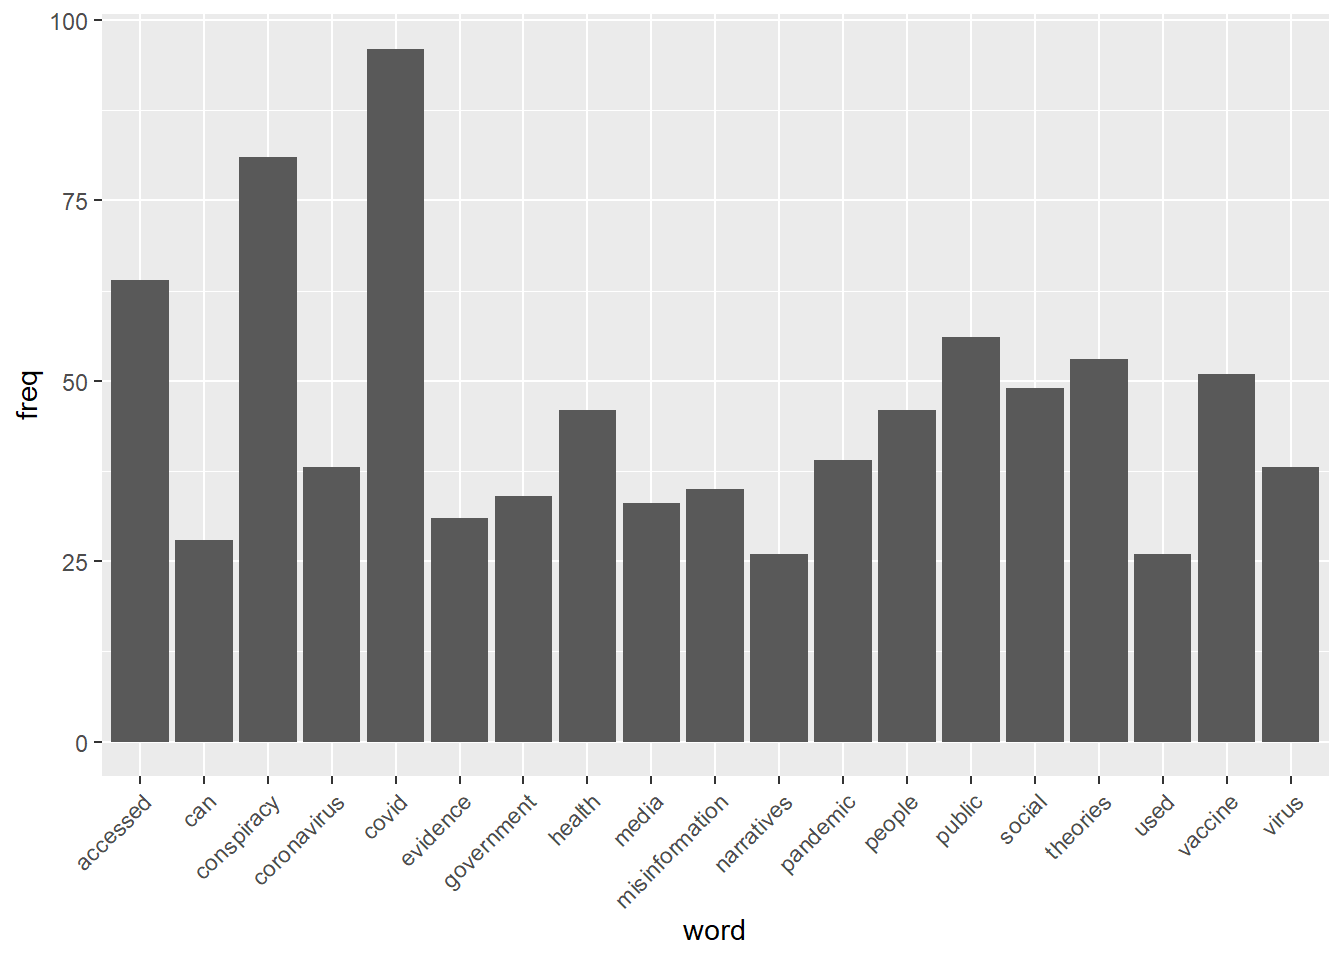
\includegraphics{book_LCC_files/figure-latex/unnamed-chunk-154-1.pdf}
Encontrar correlaciones

\begin{Shaded}
\begin{Highlighting}[]
\NormalTok{AS }\OtherTok{\textless{}{-}}\FunctionTok{findAssocs}\NormalTok{(my\_tdm, }\StringTok{"covid"}\NormalTok{, }\AttributeTok{corlimit=}\FloatTok{0.2}\NormalTok{) }

\NormalTok{AS}\SpecialCharTok{$}\NormalTok{covid}
\end{Highlighting}
\end{Shaded}

\begin{verbatim}
##         first      national         clear       similar         study 
##          0.97          0.92          0.90          0.90          0.90 
##         cause        within        causes     different        higher 
##          0.89          0.89          0.88          0.88          0.88 
##        king’s  government’s      increase          seen          note 
##          0.88          0.87          0.87          0.87          0.86 
##           put          role         shown      analysis        better 
##          0.86          0.86          0.85          0.84          0.84 
##           far         found         might       however      lockdown 
##          0.84          0.84          0.84          0.83          0.83 
##          need           see        people         trust      emerging 
##          0.83          0.83          0.82          0.82          0.81 
##        always          data   communities      pandemic   coronavirus 
##          0.80          0.79          0.78          0.78          0.77 
##      accessed      although        claims       develop    government 
##          0.76          0.76          0.76          0.76          0.76 
##         based understanding       content  deliberately        policy 
##          0.75          0.75          0.74          0.74          0.74 
##     companies       despite     emergency     following        global 
##          0.73          0.73          0.73          0.73          0.73 
##          harm      official        shared        across         china 
##          0.73          0.73          0.72          0.71          0.71 
##    statistics        future    narratives        result       support 
##          0.71          0.70          0.70          0.70          0.70 
##          will        impact       towards     according      compared 
##          0.70          0.69          0.69          0.68          0.68 
##      directly     discussed       greater        groups       largely 
##          0.68          0.68          0.68          0.68          0.68 
##         paper          play       society       twitter       beliefs 
##          0.68          0.68          0.68          0.68          0.67 
##        london          much        online          rate         april 
##          0.67          0.67          0.67          0.67          0.66 
##       country          many          also      findings          left 
##          0.65          0.65          0.64          0.64          0.64 
##         media          part         place       popular         reach 
##          0.64          0.64          0.64          0.64          0.64 
##        social        united        months       remains        theory 
##          0.64          0.64          0.62          0.62          0.61 
##      approach          less          long      credible       efforts 
##          0.60          0.60          0.60          0.58          0.58 
##           may           one         cases    conspiracy           two 
##          0.58          0.58          0.57          0.57          0.56 
##      theories      facebook     regarding       related        likely 
##          0.55          0.52          0.52          0.52          0.51 
##         still          used        almost       causing          rise 
##          0.50          0.50          0.49          0.49          0.49 
##        around          real     therefore          time        center 
##          0.48          0.48          0.48          0.48          0.47 
##         known      includes       network socioeconomic         times 
##          0.47          0.46          0.46          0.46          0.46 
##      research          work       already      identify    understand 
##          0.45          0.45          0.43          0.43          0.43 
##   individuals        report      minority     dangerous          help 
##          0.41          0.40          0.39          0.38          0.38 
##        office     including         taken          open         blame 
##          0.38          0.37          0.37          0.34          0.33 
##       college          know       leading       amongst     attention 
##          0.32          0.32          0.32          0.31          0.31 
##   authorities    categories        change         early          term 
##          0.31          0.31          0.31          0.31          0.31 
##         often  consequences       million   antivaccine        number 
##          0.30          0.28          0.28          0.27          0.27 
##        create         false         group          take    conclusion 
##          0.25          0.24          0.24          0.24          0.23 
##     community        taking 
##          0.22          0.22
\end{verbatim}

WordClouds

\begin{Shaded}
\begin{Highlighting}[]
\FunctionTok{set.seed}\NormalTok{(}\DecValTok{142}\NormalTok{)}
\NormalTok{dark2 }\OtherTok{\textless{}{-}} \FunctionTok{brewer.pal}\NormalTok{(}\DecValTok{6}\NormalTok{, }\StringTok{"Dark2"}\NormalTok{)}
\FunctionTok{wordcloud}\NormalTok{(}\FunctionTok{names}\NormalTok{(freq), freq, }\AttributeTok{max.words=}\DecValTok{35}\NormalTok{, }\AttributeTok{rot.per=}\FloatTok{0.4}\NormalTok{, }\AttributeTok{colors=}\NormalTok{dark2)}
\end{Highlighting}
\end{Shaded}

\begin{verbatim}
## Warning in wordcloud(names(freq), freq, max.words = 35, rot.per = 0.4, colors =
## dark2): conspiracy could not be fit on page. It will not be plotted.
\end{verbatim}

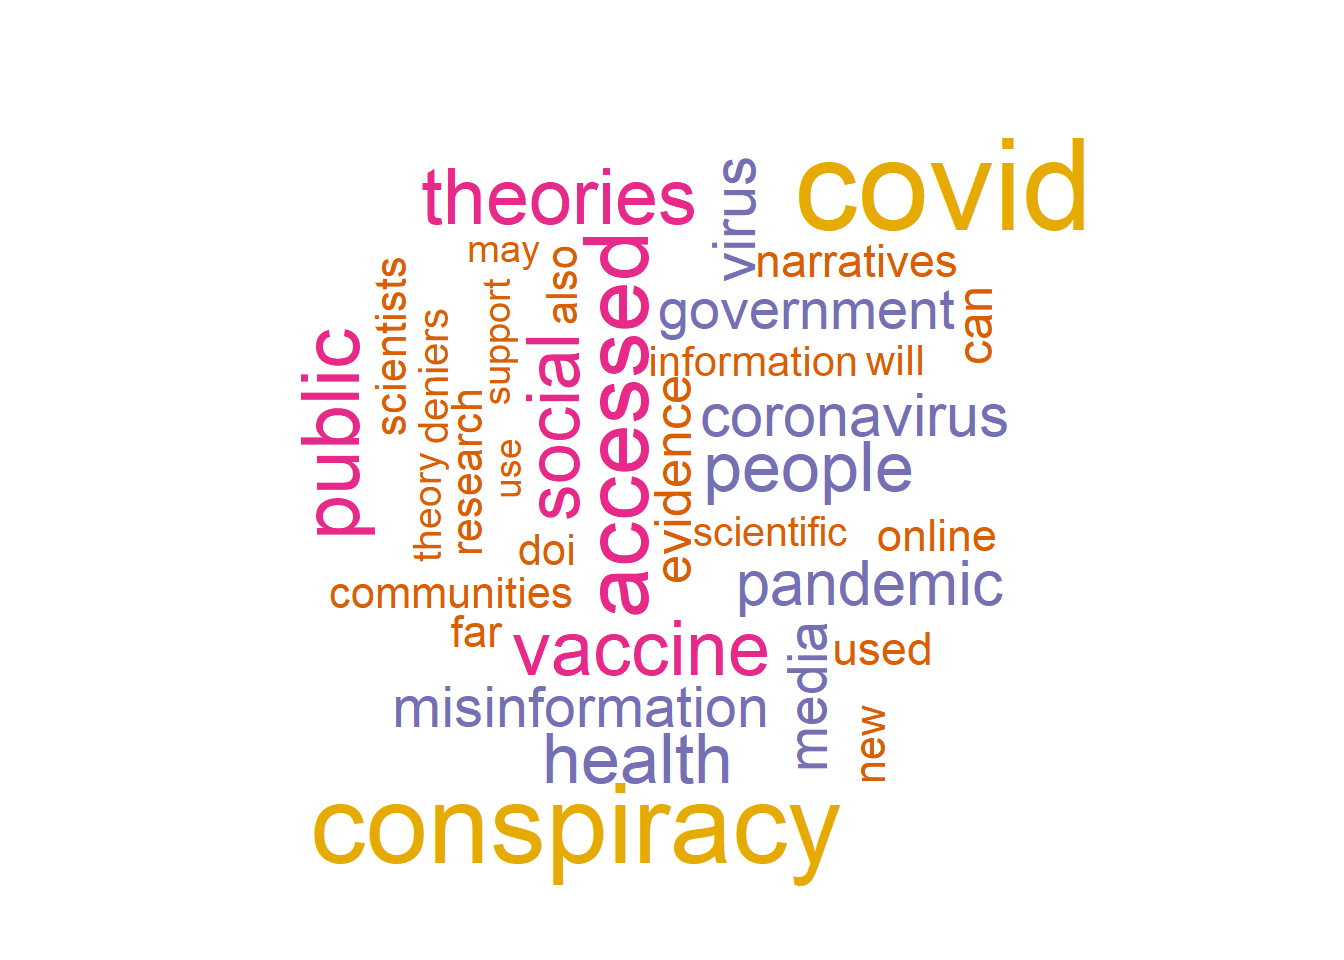
\includegraphics{book_LCC_files/figure-latex/unnamed-chunk-156-1.pdf}

Visualizamos en forma de matriz los términos que aparecen en el wordcloud anterior

\begin{Shaded}
\begin{Highlighting}[]
\NormalTok{m }\OtherTok{\textless{}{-}} \FunctionTok{as.matrix}\NormalTok{(my\_tdm)}
\NormalTok{v }\OtherTok{\textless{}{-}} \FunctionTok{sort}\NormalTok{(}\FunctionTok{rowSums}\NormalTok{(m),}\AttributeTok{decreasing=}\ConstantTok{TRUE}\NormalTok{)}
\FunctionTok{head}\NormalTok{(v,}\DecValTok{35}\NormalTok{)}
\end{Highlighting}
\end{Shaded}

\begin{verbatim}
##          covid     conspiracy       accessed         public       theories 
##             96             81             64             56             53 
##        vaccine         social         health         people       pandemic 
##             51             49             46             46             39 
##    coronavirus          virus misinformation     government          media 
##             38             38             35             34             33 
##       evidence            can     narratives           used         online 
##             31             28             26             26             25 
##            far           also    communities            doi            new 
##             24             23             23             23             23 
##       research     scientists        deniers    information           will 
##             23             23             22             22             22 
##     scientific         theory            may        support disinformation 
##             21             20             19             19             18
\end{verbatim}

\hypertarget{text-mining-2-topic-modelling}{%
\section{Text Mining 2 (Topic Modelling)}\label{text-mining-2-topic-modelling}}

En text mining normalmente tenemos colecciones de documentos, ya sean publicaciones de blogs o artículos de noticias,etc. los cuales queremos dividir en grupos naturales de forma que podamos entenderlos por separado. Topic modelling es un método para la clasificación sin supervisión de estos documentos, similar al clustering sobre datos numérico, el cual encuentra grupos naturales de items incluso cuando no estamos seguros de lo que estamos buscando.

`Latent Dirichlet allocation'(LDA) es un método particularmente popular para ajustar uun `Topic Model'. Trata cada documento como una mezcla de `topics', y cada `topic' como una mezcla de palabras. Esto permite a los documentos superponerse sobre otros en cuanto a contenido en lugar de tener que ser separados en grupos discretos, de forma que imita en cierta parte el uso natural del lenguaje.

Siendo `Latent Dirichlet allocation' uno de los algoritmos más comunes para `topic modelin', podemos entenderlo teniendo en cuenta dos principios.

\begin{itemize}
\item
  Cada documento es una mezcla de `topics'. Imaginamos que cada documento puede contener palabras de varios `topics' en proporciones particulares. Por ejemplo, en un modelo de 2 `topics' podríamos decir ``El 90\% del Documento 1 es 90\% topic A y 10\% topic B, mientras que el Documento 2 es 30\% topic A y 70\% topic B.''
\item
  Cada topic es una mezcla de palabras. Por ejemplo, podríamos imaginar un modelo de 2 `topics' de `American news', con un topic para ``politics'' y otra para ``entertainment''. Las palabras más comunes en el topic de política podrían ser ``President'', ``Congress'', y ``government'', mientras que el topic de entretenimiento podría estar formado por palabras como ``movies'', ``television'', y ``actor''. Por otro lado, podrían haber palabras compartidas por los topics; una palabra como ``budget'' podría aparecer en los dos a la vez.
\end{itemize}

En definitiva, LDA es un método matemático para estimar ambos principios al mismo tiempo: encontrar la mezcla de palabras que está asociada a cada topic, mientras que a la vez se determina la mezcla de topics que describe cada documento.

\begin{figure}
\centering
\includegraphics{https://www.tidytextmining.com/images/tmwr_0601.png}
\caption{Diagrama de flujo de `text analysis'}
\end{figure}

Tal y como se muestra en la imagen anterior, el paquete de `topic models' coge un `Document-Term Matrix' como entrada y produce un modelo que puede ser ordenado por tidytext, de tal forma que pueda ser manipulado y visualizado con dplyr y ggplot2.

A continuación vamos a aplicar Topic Modelling al conjunto de documentos del apartado 1 de TextMining.

\begin{Shaded}
\begin{Highlighting}[]
\FunctionTok{library}\NormalTok{(tm)}
\FunctionTok{library}\NormalTok{(pdftools)}
\FunctionTok{library}\NormalTok{(stringr)}
\FunctionTok{library}\NormalTok{(stringi)}
\FunctionTok{library}\NormalTok{(ggplot2)}
\FunctionTok{library}\NormalTok{(RColorBrewer)}
\FunctionTok{library}\NormalTok{(wordcloud)}
\FunctionTok{library}\NormalTok{(topicmodels)}
\end{Highlighting}
\end{Shaded}

\begin{verbatim}
## Warning: package 'topicmodels' was built under R version 4.0.5
\end{verbatim}

\begin{Shaded}
\begin{Highlighting}[]
\FunctionTok{library}\NormalTok{(tidytext)}
\end{Highlighting}
\end{Shaded}

\begin{verbatim}
## Warning: package 'tidytext' was built under R version 4.0.5
\end{verbatim}

\begin{Shaded}
\begin{Highlighting}[]
\FunctionTok{library}\NormalTok{(reshape2)}
\end{Highlighting}
\end{Shaded}

\begin{verbatim}
## Warning: package 'reshape2' was built under R version 4.0.5
\end{verbatim}

\begin{verbatim}
## 
## Attaching package: 'reshape2'
\end{verbatim}

\begin{verbatim}
## The following object is masked from 'package:tidyr':
## 
##     smiths
\end{verbatim}

\begin{Shaded}
\begin{Highlighting}[]
\FunctionTok{library}\NormalTok{(ggplot2)}
\FunctionTok{library}\NormalTok{(dplyr)}
\FunctionTok{library}\NormalTok{(tidyr)}
\end{Highlighting}
\end{Shaded}

\begin{Shaded}
\begin{Highlighting}[]
\NormalTok{directorio.textos }\OtherTok{\textless{}{-}} \FunctionTok{file.path}\NormalTok{(}\StringTok{"C:"}\NormalTok{, }\StringTok{"pdfstextmining2021"}\NormalTok{)}
\NormalTok{directorio.textos}
\end{Highlighting}
\end{Shaded}

\begin{verbatim}
## [1] "C:/pdfstextmining2021"
\end{verbatim}

\begin{Shaded}
\begin{Highlighting}[]
\FunctionTok{dir}\NormalTok{(directorio.textos)}
\end{Highlighting}
\end{Shaded}

\begin{verbatim}
##  [1] "20200512_conspiracies_covid19.pdf"                                                            
##  [2] "780.2.full.pdf"                                                                               
##  [3] "bmj.n352.full.pdf"                                                                            
##  [4] "ccdrv46i1112a11-eng.pdf"                                                                      
##  [5] "CCE_Briefing_Note_001.pdf"                                                                    
##  [6] "Coronavirus_The_spread_of_misinformation.pdf"                                                 
##  [7] "COVID-19-Mistrust-and-Denial-Factsheet_RCCE-interagency-TWG.pdf"                              
##  [8] "COVID-19_and_The_Rights_of_Persons_with_Disabilities.pdf"                                     
##  [9] "COVID-19_pandemic-_Perception,_confusion_and_consp.pdf"                                       
## [10] "el-mundo-mapfre-110-en.pdf"                                                                   
## [11] "Full_book_FINAL_EN2.0-UNIDO.pdf"                                                              
## [12] "GHSN Policy Report 1.pdf"                                                                     
## [13] "how_to_respond_to_covid-19_deniers.pdf"                                                       
## [14] "ijerph-17-07818.pdf"                                                                          
## [15] "IJHPM38801596396600.pdf"                                                                      
## [16] "Imhoff-Lamberty_COVID-19-Conspiracies_Preprint.v4.pdf"                                        
## [17] "Losers in the crisis_ Europe&#8217;s radical right wing in the COVID-19 pandemic.pdf"         
## [18] "s41590-021-00875-8.pdf"                                                                       
## [19] "socsci-09-00165.pdf"                                                                          
## [20] "Tony Blair Institute, From the Fringes to the Forefront, Far Right Movements and Covid-19.pdf"
## [21] "victims-of-the-pandemic-european-far-right-parties-and-covid-19.pdf"                          
## [22] "Vocal-vaccine-deniers-guidance-document.pdf"
\end{verbatim}

\begin{Shaded}
\begin{Highlighting}[]
\NormalTok{list.files }\OtherTok{\textless{}{-}} \FunctionTok{DirSource}\NormalTok{(directorio.textos)}

\NormalTok{texts }\OtherTok{\textless{}{-}} \FunctionTok{lapply}\NormalTok{(list.files, pdf\_text) }
\end{Highlighting}
\end{Shaded}

\begin{verbatim}
## PDF error: Invalid Font Weight
## PDF error: Invalid Font Weight
## PDF error: Invalid Font Weight
## PDF error: Invalid Font Weight
## PDF error: Invalid Font Weight
## PDF error: Invalid Font Weight
## PDF error: Invalid Font Weight
\end{verbatim}

\begin{Shaded}
\begin{Highlighting}[]
\FunctionTok{length}\NormalTok{(texts)}
\end{Highlighting}
\end{Shaded}

\begin{verbatim}
## [1] 6
\end{verbatim}

\begin{Shaded}
\begin{Highlighting}[]
\FunctionTok{lapply}\NormalTok{(texts, length)}
\end{Highlighting}
\end{Shaded}

\begin{verbatim}
## $encoding
## [1] 8
## 
## $length
## [1] 4
## 
## $position
## [1] 2
## 
## $reader
## [1] 4
## 
## $mode
## [1] 17
## 
## $filelist
## [1] 2
\end{verbatim}

\begin{Shaded}
\begin{Highlighting}[]
\CommentTok{\#Crear corpus}
\NormalTok{my\_corpus }\OtherTok{\textless{}{-}} \FunctionTok{VCorpus}\NormalTok{(}\FunctionTok{VectorSource}\NormalTok{(texts))}
\NormalTok{my\_corpus}
\end{Highlighting}
\end{Shaded}

\begin{verbatim}
## <<VCorpus>>
## Metadata:  corpus specific: 0, document level (indexed): 0
## Content:  documents: 6
\end{verbatim}

\begin{Shaded}
\begin{Highlighting}[]
\CommentTok{\#Definimos la función to\_TDM que transforma un corpus en una matriz TDM (Term Document Matrix)}
\NormalTok{to\_TDM }\OtherTok{\textless{}{-}} \ControlFlowTok{function}\NormalTok{(my\_corpus)\{}
\NormalTok{  my\_tdm }\OtherTok{\textless{}{-}} \FunctionTok{DocumentTermMatrix}\NormalTok{(my\_corpus, }
                                   \AttributeTok{control =} 
                                     \FunctionTok{list}\NormalTok{(}\AttributeTok{removePunctuation =} \ConstantTok{TRUE}\NormalTok{,}
                                          \AttributeTok{stopwords =} \ConstantTok{TRUE}\NormalTok{,}
                                          \AttributeTok{tolower =} \ConstantTok{TRUE}\NormalTok{,}
                                          \AttributeTok{stemming =} \ConstantTok{FALSE}\NormalTok{,}
                                          \AttributeTok{removeNumbers =} \ConstantTok{TRUE}\NormalTok{,}
                                          \AttributeTok{bounds =} \FunctionTok{list}\NormalTok{(}\AttributeTok{global =} \FunctionTok{c}\NormalTok{(}\DecValTok{3}\NormalTok{, }\ConstantTok{Inf}\NormalTok{))))}
\NormalTok{\}         }
\end{Highlighting}
\end{Shaded}

\begin{Shaded}
\begin{Highlighting}[]
\CommentTok{\#Convertimos a TDM el corpus}
\NormalTok{my\_tdm }\OtherTok{\textless{}{-}} \FunctionTok{to\_TDM}\NormalTok{(my\_corpus)}
\end{Highlighting}
\end{Shaded}

La función LDA devuelve un un objeto que contiene todos los detalles del ajuste del modelo, como cuántas palabras están asociadas con topics y cómo los topics están asociados con los documentos

\begin{Shaded}
\begin{Highlighting}[]
\CommentTok{\# set a seed so that the output of the model is predictable}
\NormalTok{ap\_lda }\OtherTok{\textless{}{-}} \FunctionTok{LDA}\NormalTok{(my\_tdm, }\AttributeTok{k =} \DecValTok{3}\NormalTok{, }\AttributeTok{control =} \FunctionTok{list}\NormalTok{(}\AttributeTok{seed =} \DecValTok{1234}\NormalTok{))}
\NormalTok{ap\_lda}
\end{Highlighting}
\end{Shaded}

\begin{verbatim}
## A LDA_VEM topic model with 3 topics.
\end{verbatim}

El paquete tidytext proporciona el siguiente método para extraer las probabilidades de los tópicos y las palabras.

\begin{Shaded}
\begin{Highlighting}[]
\NormalTok{ap\_topics }\OtherTok{\textless{}{-}} \FunctionTok{tidy}\NormalTok{(ap\_lda, }\AttributeTok{matrix =} \StringTok{"beta"}\NormalTok{)}
\NormalTok{ap\_topics}
\end{Highlighting}
\end{Shaded}

\begin{verbatim}
## # A tibble: 894 x 3
##    topic term               beta
##    <int> <chr>             <dbl>
##  1     1 access    0.00186      
##  2     2 access    0.00665      
##  3     3 access    0.0000499    
##  4     1 accessed  0.0351       
##  5     2 accessed  0.0000000940 
##  6     3 accessed  0.0104       
##  7     1 according 0.00123      
##  8     2 according 0.00135      
##  9     3 according 0.00000000735
## 10     1 across    0.00665      
## # ... with 884 more rows
\end{verbatim}

A partir del resultado anterior podemos decir que el término ``access'' tiene 1.860677e-03 de probabilidad de ser generado en el topic 1, pero una probabilidad de 6.650884e-03 de ser generado en el topic 2.

\begin{Shaded}
\begin{Highlighting}[]
\NormalTok{ap\_top\_terms }\OtherTok{\textless{}{-}}\NormalTok{ ap\_topics }\SpecialCharTok{\%\textgreater{}\%}
  \FunctionTok{group\_by}\NormalTok{(topic) }\SpecialCharTok{\%\textgreater{}\%}
  \FunctionTok{slice\_max}\NormalTok{(beta, }\AttributeTok{n =} \DecValTok{10}\NormalTok{) }\SpecialCharTok{\%\textgreater{}\%} 
  \FunctionTok{ungroup}\NormalTok{() }\SpecialCharTok{\%\textgreater{}\%}
  \FunctionTok{arrange}\NormalTok{(topic, }\SpecialCharTok{{-}}\NormalTok{beta)}

\NormalTok{ap\_top\_terms }\SpecialCharTok{\%\textgreater{}\%}
  \FunctionTok{mutate}\NormalTok{(}\AttributeTok{term =} \FunctionTok{reorder\_within}\NormalTok{(term, beta, topic)) }\SpecialCharTok{\%\textgreater{}\%}
  \FunctionTok{ggplot}\NormalTok{(}\FunctionTok{aes}\NormalTok{(beta, term, }\AttributeTok{fill =} \FunctionTok{factor}\NormalTok{(topic))) }\SpecialCharTok{+}
  \FunctionTok{geom\_col}\NormalTok{(}\AttributeTok{show.legend =} \ConstantTok{FALSE}\NormalTok{) }\SpecialCharTok{+}
  \FunctionTok{facet\_wrap}\NormalTok{(}\SpecialCharTok{\textasciitilde{}}\NormalTok{ topic, }\AttributeTok{scales =} \StringTok{"free"}\NormalTok{) }\SpecialCharTok{+}
  \FunctionTok{scale\_y\_reordered}\NormalTok{()}
\end{Highlighting}
\end{Shaded}

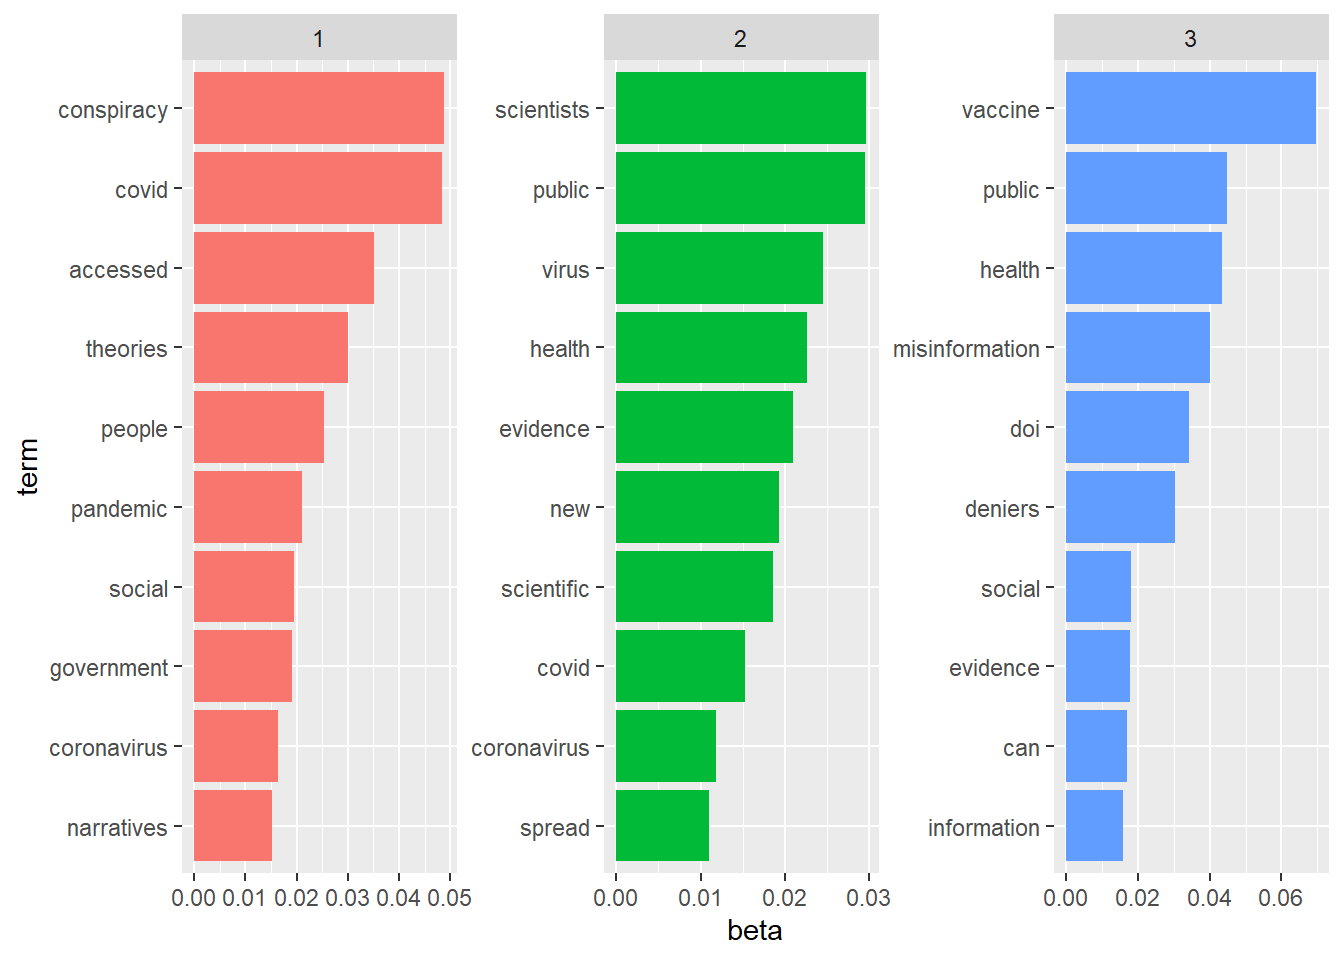
\includegraphics{book_LCC_files/figure-latex/unnamed-chunk-167-1.pdf}

Gracias a esta visualización podemos entender mejor los topics extraídos de los documentos. Las palabras más comunes en el topic 1 fueron ``conspiracy'', ``covid'', ``accessed'' y ``theories'', lo que hace pensar que lo que sugiere el documento es que el covid es una teoría conspiratoria. Por otro lado, las palabras más comunes en el topic 2 fueron ``scientists'', ``public'', ``virus'' y ``health'', lo que hace pensar que lo que sugiere el documento es que la salud pública y los científicos tuvieron relevancia con el virus, y por último, las palabras más comunes en el topic 3 fueron ``vaccine'', ``public'', ``health'' y ``misinformation'', lo que hace pensar que lo que sugiere el documento es que hay mucha desinformación acerca de las vacunas entre la gente.

\begin{Shaded}
\begin{Highlighting}[]
\NormalTok{ap\_lda\_2 }\OtherTok{\textless{}{-}} \FunctionTok{LDA}\NormalTok{(my\_tdm, }\AttributeTok{k =} \DecValTok{2}\NormalTok{, }\AttributeTok{control =} \FunctionTok{list}\NormalTok{(}\AttributeTok{seed =} \DecValTok{1234}\NormalTok{))}
\NormalTok{ap\_lda\_2}
\end{Highlighting}
\end{Shaded}

\begin{verbatim}
## A LDA_VEM topic model with 2 topics.
\end{verbatim}

\begin{Shaded}
\begin{Highlighting}[]
\NormalTok{ap\_topics\_2 }\OtherTok{\textless{}{-}} \FunctionTok{tidy}\NormalTok{(ap\_lda\_2, }\AttributeTok{matrix =} \StringTok{"beta"}\NormalTok{)}
\NormalTok{ap\_topics\_2}
\end{Highlighting}
\end{Shaded}

\begin{verbatim}
## # A tibble: 596 x 3
##    topic term          beta
##    <int> <chr>        <dbl>
##  1     1 access    0.00167 
##  2     2 access    0.00410 
##  3     1 accessed  0.0317  
##  4     2 accessed  0.00563 
##  5     1 according 0.00125 
##  6     2 according 0.000610
##  7     1 across    0.00635 
##  8     2 across    0.00128 
##  9     1 address   0.000577
## 10     2 address   0.00655 
## # ... with 586 more rows
\end{verbatim}

Como alternativa, se pueden usar los términos que tuvieron la mayor diferencia en `beta' entre los topics 1 y 2. Esto se puede estimar basándonos en el log ratio de los 2. Para restringirlo a un set de palabras muy relevantes podemos filtrar por palabras muy relativamente comunes, que son aquellas con un `beta' mayor que 1/1000 por lo menos en un topic.

\begin{Shaded}
\begin{Highlighting}[]
\NormalTok{beta\_wide }\OtherTok{\textless{}{-}}\NormalTok{ ap\_topics\_2 }\SpecialCharTok{\%\textgreater{}\%}
  \FunctionTok{mutate}\NormalTok{(}\AttributeTok{topic =} \FunctionTok{paste0}\NormalTok{(}\StringTok{"topic"}\NormalTok{, topic)) }\SpecialCharTok{\%\textgreater{}\%}
  \FunctionTok{pivot\_wider}\NormalTok{(}\AttributeTok{names\_from =}\NormalTok{ topic, }\AttributeTok{values\_from =}\NormalTok{ beta) }\SpecialCharTok{\%\textgreater{}\%} 
  \FunctionTok{filter}\NormalTok{(topic1 }\SpecialCharTok{\textgreater{}}\NormalTok{ .}\DecValTok{001} \SpecialCharTok{|}\NormalTok{ topic2 }\SpecialCharTok{\textgreater{}}\NormalTok{ .}\DecValTok{001}\NormalTok{) }\SpecialCharTok{\%\textgreater{}\%}
  \FunctionTok{mutate}\NormalTok{(}\AttributeTok{log\_ratio =} \FunctionTok{log2}\NormalTok{(topic2 }\SpecialCharTok{/}\NormalTok{ topic1))}

\NormalTok{beta\_wide}
\end{Highlighting}
\end{Shaded}

\begin{verbatim}
## # A tibble: 298 x 4
##    term        topic1   topic2 log_ratio
##    <chr>        <dbl>    <dbl>     <dbl>
##  1 access    0.00167  0.00410      1.29 
##  2 accessed  0.0317   0.00563     -2.49 
##  3 according 0.00125  0.000610    -1.04 
##  4 across    0.00635  0.00128     -2.31 
##  5 address   0.000577 0.00655      3.50 
##  6 almost    0.00271  0.000919    -1.56 
##  7 already   0.00253  0.00202     -0.326
##  8 also      0.0101   0.00398     -1.34 
##  9 although  0.00323  0.000972    -1.73 
## 10 always    0.00252  0.000378    -2.74 
## # ... with 288 more rows
\end{verbatim}

Y por último visualizamos las palabras con las diferencias más grandes observadas entre los dos topics en la siguiente gráfica:

\begin{Shaded}
\begin{Highlighting}[]
\NormalTok{beta\_wide }\SpecialCharTok{\%\textgreater{}\%}
  \FunctionTok{group\_by}\NormalTok{(}\AttributeTok{direction =}\NormalTok{ log\_ratio }\SpecialCharTok{\textgreater{}} \DecValTok{0}\NormalTok{) }\SpecialCharTok{\%\textgreater{}\%}
  \FunctionTok{slice\_max}\NormalTok{(}\FunctionTok{abs}\NormalTok{(log\_ratio), }\AttributeTok{n =} \DecValTok{10}\NormalTok{) }\SpecialCharTok{\%\textgreater{}\%} 
  \FunctionTok{ungroup}\NormalTok{() }\SpecialCharTok{\%\textgreater{}\%}
  \FunctionTok{mutate}\NormalTok{(}\AttributeTok{term =} \FunctionTok{reorder}\NormalTok{(term, log\_ratio)) }\SpecialCharTok{\%\textgreater{}\%}
  \FunctionTok{ggplot}\NormalTok{(}\FunctionTok{aes}\NormalTok{(log\_ratio, term)) }\SpecialCharTok{+}
  \FunctionTok{geom\_col}\NormalTok{() }\SpecialCharTok{+}
  \FunctionTok{labs}\NormalTok{(}\AttributeTok{x =} \StringTok{"Log2 ratio of beta in topic 2 / topic 1"}\NormalTok{, }\AttributeTok{y =} \ConstantTok{NULL}\NormalTok{)}
\end{Highlighting}
\end{Shaded}

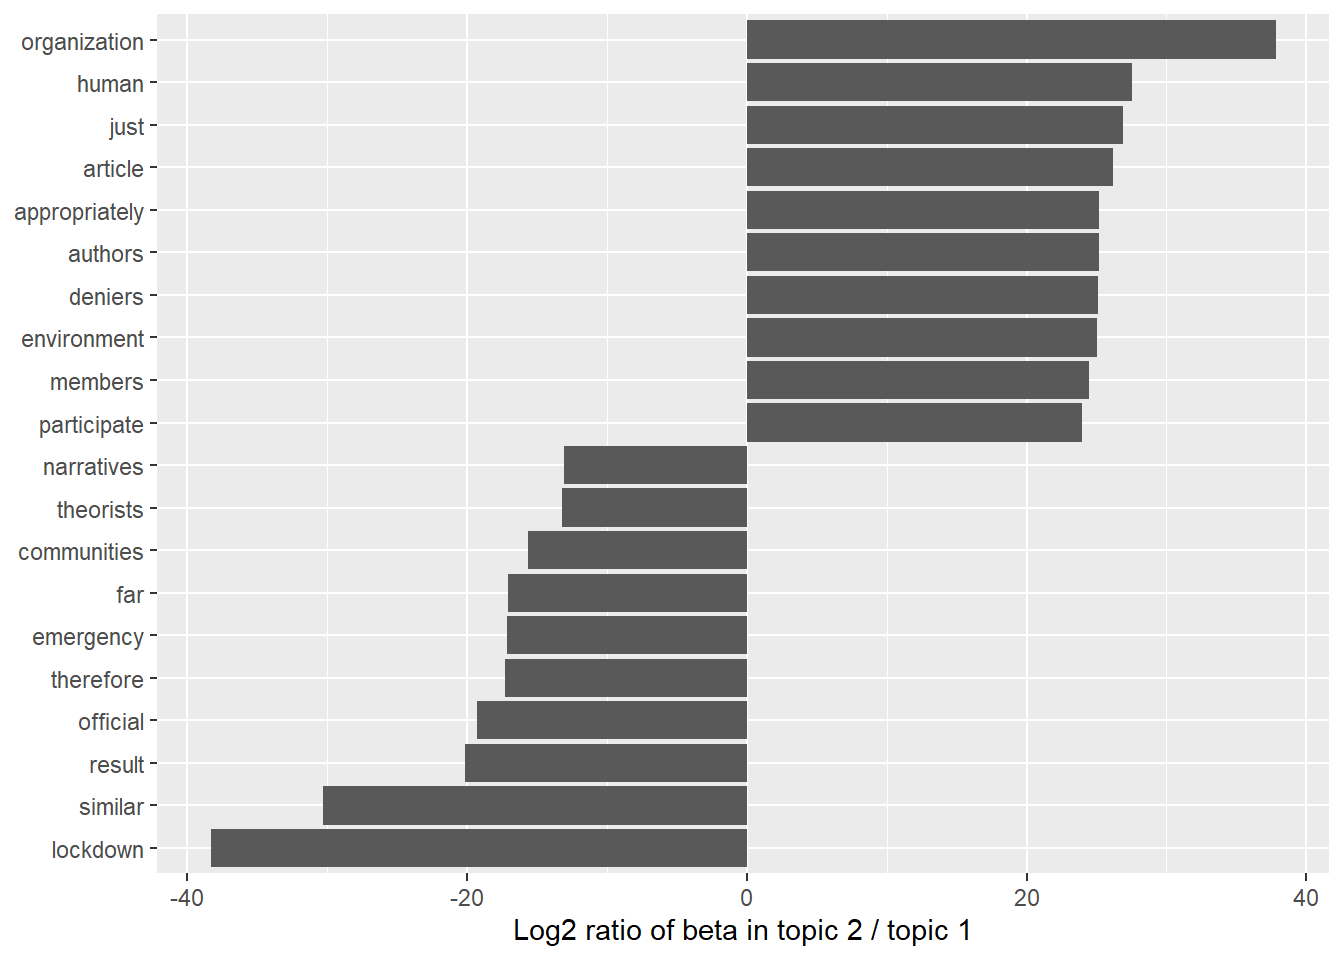
\includegraphics{book_LCC_files/figure-latex/unnamed-chunk-170-1.pdf}

\hypertarget{social-network-analysis---gameofthrones}{%
\chapter{Social Network Analysis - GameOfThrones}\label{social-network-analysis---gameofthrones}}

\begin{Shaded}
\begin{Highlighting}[]
\FunctionTok{library}\NormalTok{(tidyverse)}

\FunctionTok{library}\NormalTok{(igraph)}
\end{Highlighting}
\end{Shaded}

\begin{verbatim}
## 
## Attaching package: 'igraph'
\end{verbatim}

\begin{verbatim}
## The following object is masked from 'package:arules':
## 
##     union
\end{verbatim}

\begin{verbatim}
## The following objects are masked from 'package:lubridate':
## 
##     %--%, union
\end{verbatim}

\begin{verbatim}
## The following objects are masked from 'package:dplyr':
## 
##     as_data_frame, groups, union
\end{verbatim}

\begin{verbatim}
## The following objects are masked from 'package:purrr':
## 
##     compose, simplify
\end{verbatim}

\begin{verbatim}
## The following object is masked from 'package:tidyr':
## 
##     crossing
\end{verbatim}

\begin{verbatim}
## The following object is masked from 'package:tibble':
## 
##     as_data_frame
\end{verbatim}

\begin{verbatim}
## The following objects are masked from 'package:stats':
## 
##     decompose, spectrum
\end{verbatim}

\begin{verbatim}
## The following object is masked from 'package:base':
## 
##     union
\end{verbatim}

\begin{Shaded}
\begin{Highlighting}[]
\CommentTok{\#load("C:/Users/Guillermo/Desktop/CURSO 2020{-}2021/SEGUNDO CUATRIMESTRE/LABORATORIO DE COMPUTACION CIENTIFICA/GameOfThrones/union\_edges.RData")}
\CommentTok{\#load("C:/Users/Guillermo/Desktop/CURSO 2020{-}2021/SEGUNDO CUATRIMESTRE/LABORATORIO DE COMPUTACION CIENTIFICA/GameOfThrones/union\_characters.RData")}

\FunctionTok{load}\NormalTok{(}\StringTok{"union\_edges.RData"}\NormalTok{)}

\FunctionTok{load}\NormalTok{(}\StringTok{"union\_characters.RData"}\NormalTok{)}
\end{Highlighting}
\end{Shaded}

\begin{Shaded}
\begin{Highlighting}[]
\FunctionTok{head}\NormalTok{(union\_edges)}
\end{Highlighting}
\end{Shaded}

\begin{verbatim}
##               source            target   type   color   lty
## 1         Lysa Arryn      Robert Arryn mother #7570B3 solid
## 2       Jasper Arryn        Alys Arryn father #1B9E77 solid
## 3       Jasper Arryn         Jon Arryn father #1B9E77 solid
## 4          Jon Arryn      Robert Arryn father #1B9E77 solid
## 110 Cersei Lannister  Tommen Baratheon mother #7570B3 solid
## 210 Cersei Lannister Joffrey Baratheon mother #7570B3 solid
\end{verbatim}

\begin{Shaded}
\begin{Highlighting}[]
\FunctionTok{head}\NormalTok{(union\_characters)}
\end{Highlighting}
\end{Shaded}

\begin{verbatim}
##            name male culture          house popularity      house2   color
## 1    Alys Arryn    0    <NA>    House Arryn 0.08026756        <NA>    <NA>
## 2 Elys Waynwood    0    <NA> House Waynwood 0.07023411        <NA>    <NA>
## 3  Jasper Arryn    1    <NA>    House Arryn 0.04347826        <NA>    <NA>
## 4   Jeyne Royce    0    <NA>    House Royce 0.00000000        <NA>    <NA>
## 5     Jon Arryn    1 Valemen    House Arryn 0.83612040        <NA>    <NA>
## 6    Lysa Arryn    0    <NA>    House Tully 0.00000000 House Tully #F781BF
##    shape
## 1 circle
## 2 circle
## 3 square
## 4 circle
## 5 square
## 6 circle
\end{verbatim}

\begin{Shaded}
\begin{Highlighting}[]
\NormalTok{union\_graph }\OtherTok{\textless{}{-}} \FunctionTok{graph\_from\_data\_frame}\NormalTok{(union\_edges, }\AttributeTok{directed =} \ConstantTok{TRUE}\NormalTok{, }\AttributeTok{vertices =}\NormalTok{ union\_characters)}
\CommentTok{\# Alguna información}
\NormalTok{union\_graph }\CommentTok{\# Mirar las propiedades}
\end{Highlighting}
\end{Shaded}

\begin{verbatim}
## IGRAPH a9be701 DN-- 208 404 -- 
## + attr: name (v/c), male (v/n), culture (v/c), house (v/c), popularity
## | (v/n), house2 (v/c), color (v/c), shape (v/c), type (e/c), color
## | (e/c), lty (e/c)
## + edges from a9be701 (vertex names):
##  [1] Lysa Arryn       ->Robert Arryn       Jasper Arryn     ->Alys Arryn        
##  [3] Jasper Arryn     ->Jon Arryn          Jon Arryn        ->Robert Arryn      
##  [5] Cersei Lannister ->Tommen Baratheon   Cersei Lannister ->Joffrey Baratheon 
##  [7] Cassana Baratheon->Stannis Baratheon  Cersei Lannister ->Myrcella Baratheon
##  [9] Selyse Florent   ->Shireen Baratheon  Cassana Baratheon->Renly Baratheon   
## [11] Rhaelle Targaryen->Steffon Baratheon  Cassana Baratheon->Robert Baratheon  
## + ... omitted several edges
\end{verbatim}

\begin{Shaded}
\begin{Highlighting}[]
\FunctionTok{sort}\NormalTok{(}\FunctionTok{V}\NormalTok{(union\_graph)}\SpecialCharTok{$}\NormalTok{popularity,}\AttributeTok{decreasing =} \ConstantTok{TRUE}\NormalTok{)}\CommentTok{\# información que tenemos en los vértices}
\end{Highlighting}
\end{Shaded}

\begin{verbatim}
##   [1] 1.00000000 1.00000000 1.00000000 1.00000000 1.00000000 1.00000000
##   [7] 1.00000000 1.00000000 1.00000000 1.00000000 1.00000000 1.00000000
##  [13] 1.00000000 1.00000000 1.00000000 1.00000000 1.00000000 1.00000000
##  [19] 1.00000000 0.97993311 0.89632107 0.86956522 0.85618729 0.83612040
##  [25] 0.79933110 0.77257525 0.73913043 0.73913043 0.70903010 0.70568562
##  [31] 0.69565217 0.66555184 0.65551839 0.62207358 0.56187291 0.55852843
##  [37] 0.55183946 0.51170569 0.49832776 0.49498328 0.49498328 0.48494983
##  [43] 0.47826087 0.45819398 0.44481605 0.44147157 0.43478261 0.42474916
##  [49] 0.40133779 0.39799331 0.37792642 0.37123746 0.35451505 0.34782609
##  [55] 0.33110368 0.32775920 0.32107023 0.32107023 0.29096990 0.28762542
##  [61] 0.27090301 0.24749164 0.24414716 0.23745819 0.23745819 0.23411371
##  [67] 0.23076923 0.23076923 0.23076923 0.22742475 0.21739130 0.21739130
##  [73] 0.21739130 0.21404682 0.21070234 0.20735786 0.19063545 0.17391304
##  [79] 0.17056856 0.17056856 0.17056856 0.17056856 0.16722408 0.16387960
##  [85] 0.16387960 0.16053512 0.16053512 0.15719064 0.15384615 0.15384615
##  [91] 0.14381271 0.14046823 0.14046823 0.14046823 0.14046823 0.14046823
##  [97] 0.13712375 0.13712375 0.13712375 0.13712375 0.13712375 0.13377926
## [103] 0.13043478 0.13043478 0.13043478 0.12709030 0.12709030 0.12709030
## [109] 0.12709030 0.12040134 0.12040134 0.11705686 0.11705686 0.11371237
## [115] 0.11036789 0.10702341 0.10702341 0.10367893 0.10367893 0.10367893
## [121] 0.10367893 0.10033445 0.09030100 0.08695652 0.08361204 0.08361204
## [127] 0.08361204 0.08361204 0.08026756 0.08026756 0.08026756 0.08026756
## [133] 0.07692308 0.07692308 0.07357860 0.07357860 0.07357860 0.07023411
## [139] 0.07023411 0.07023411 0.06688963 0.06688963 0.06688963 0.06688963
## [145] 0.06354515 0.06354515 0.06354515 0.06354515 0.06020067 0.06020067
## [151] 0.06020067 0.05016722 0.05016722 0.05016722 0.04682274 0.04347826
## [157] 0.04347826 0.04013378 0.03678930 0.03344482 0.00000000 0.00000000
## [163] 0.00000000 0.00000000 0.00000000 0.00000000 0.00000000 0.00000000
## [169] 0.00000000 0.00000000 0.00000000 0.00000000 0.00000000 0.00000000
## [175] 0.00000000 0.00000000 0.00000000 0.00000000 0.00000000 0.00000000
## [181] 0.00000000 0.00000000 0.00000000 0.00000000 0.00000000 0.00000000
## [187] 0.00000000 0.00000000 0.00000000 0.00000000 0.00000000 0.00000000
## [193] 0.00000000 0.00000000 0.00000000 0.00000000 0.00000000 0.00000000
## [199] 0.00000000 0.00000000 0.00000000 0.00000000 0.00000000 0.00000000
## [205] 0.00000000 0.00000000 0.00000000 0.00000000
\end{verbatim}

\begin{Shaded}
\begin{Highlighting}[]
\FunctionTok{plot}\NormalTok{(union\_graph)}
\end{Highlighting}
\end{Shaded}

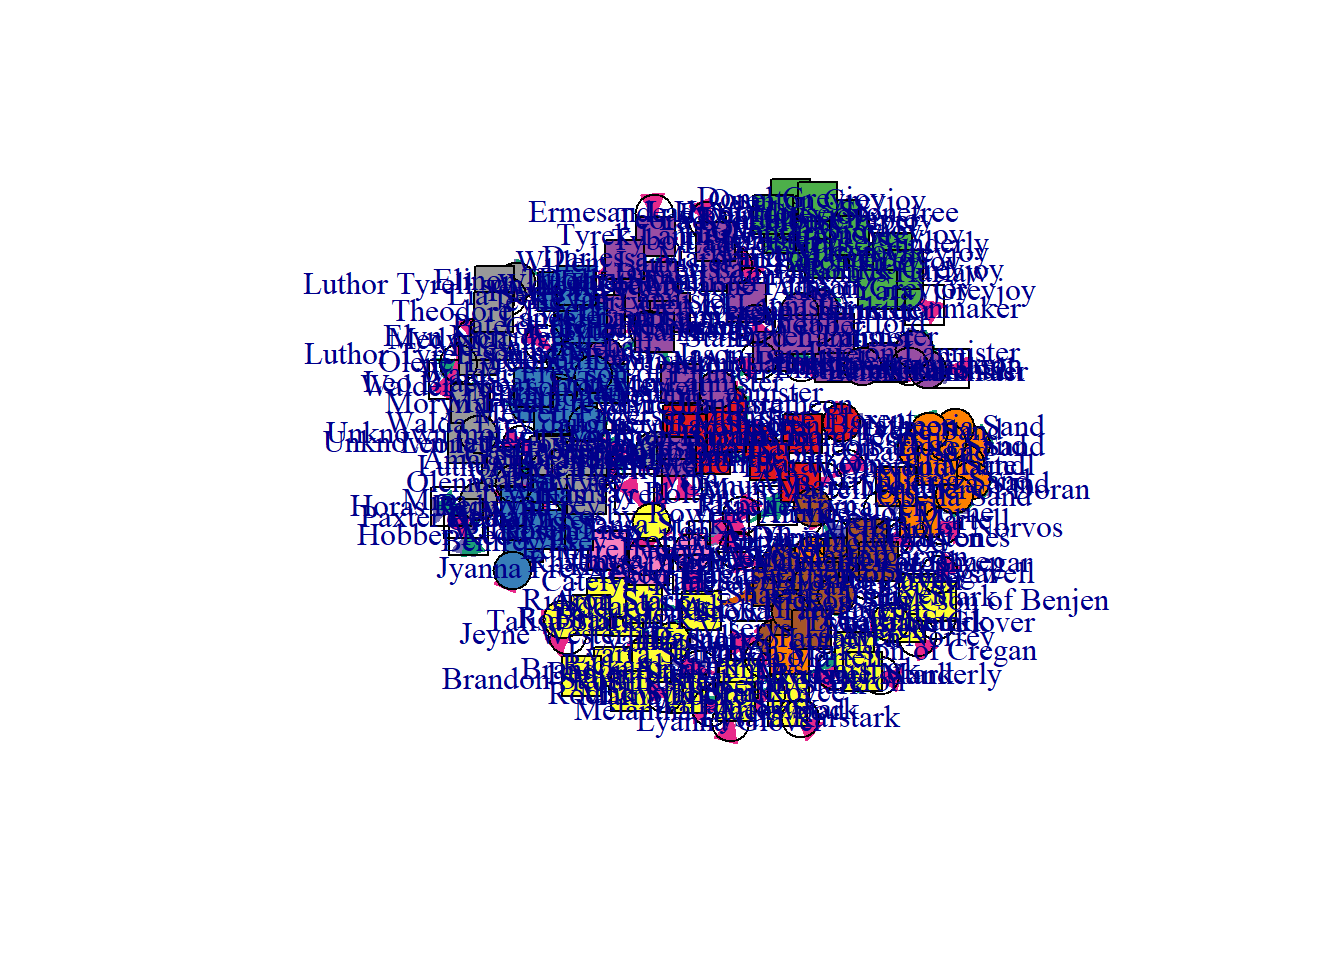
\includegraphics{book_LCC_files/figure-latex/unnamed-chunk-176-1.pdf}

¿Cuales son los personajes 10 más populares?

\begin{Shaded}
\begin{Highlighting}[]
\NormalTok{popularidad }\OtherTok{\textless{}{-}} \FunctionTok{V}\NormalTok{(union\_graph)}\SpecialCharTok{$}\NormalTok{popularity}
\NormalTok{indices }\OtherTok{\textless{}{-}} \FunctionTok{order}\NormalTok{(popularidad,}\AttributeTok{decreasing =} \ConstantTok{TRUE}\NormalTok{)}

\NormalTok{personajes\_populares }\OtherTok{\textless{}{-}} \FunctionTok{V}\NormalTok{(union\_graph)[indices]}
\NormalTok{personajes\_populares[}\DecValTok{1}\SpecialCharTok{:}\DecValTok{10}\NormalTok{]}
\end{Highlighting}
\end{Shaded}

\begin{verbatim}
## + 10/208 vertices, named, from a9be701:
##  [1] Cersei Lannister  Jaime Lannister   Joffrey Baratheon Margaery Tyrell  
##  [5] Renly Baratheon   Stannis Baratheon Tommen Baratheon  Theon Greyjoy    
##  [9] Sansa Stark       Tyrion Lannister
\end{verbatim}

Aplica al grafo page.rank. ¿En qué posición está Jon Snow según esta medida?

\begin{Shaded}
\begin{Highlighting}[]
\NormalTok{pageRankGrafo}\OtherTok{\textless{}{-}} \FunctionTok{page.rank}\NormalTok{(union\_graph)}\SpecialCharTok{$}\NormalTok{vector}
\FunctionTok{match}\NormalTok{(pageRankGrafo[}\StringTok{"Jon Snow"}\NormalTok{], pageRankGrafo)}
\end{Highlighting}
\end{Shaded}

\begin{verbatim}
## [1] 145
\end{verbatim}

Calcula el personaje que está a mayor y menor distancia de Arya Stark.

\begin{Shaded}
\begin{Highlighting}[]
\NormalTok{V }\OtherTok{\textless{}{-}} \FunctionTok{sort}\NormalTok{(}\FunctionTok{distances}\NormalTok{(union\_graph)[}\StringTok{"Arya Stark"}\NormalTok{,])}
\NormalTok{V}\SpecialCharTok{!=}\ConstantTok{Inf}
\end{Highlighting}
\end{Shaded}

\begin{verbatim}
##                            Arya Stark                         Catelyn Stark 
##                                  TRUE                                  TRUE 
##                          Eddard Stark                           Sansa Stark 
##                                  TRUE                                  TRUE 
##                            Bran Stark                              Jon Snow 
##                                  TRUE                                  TRUE 
##                          Lyarra Stark                         Rickard Stark 
##                                  TRUE                                  TRUE 
##                          Rickon Stark                            Robb Stark 
##                                  TRUE                                  TRUE 
##                          Hoster Tully                          Minisa Whent 
##                                  TRUE                                  TRUE 
##                            Lysa Arryn                          Edmure Tully 
##                                  TRUE                                  TRUE 
##                      Tyrion Lannister                     Rhaegar Targaryen 
##                                  TRUE                                  TRUE 
##                            Arya Flint                          Benjen Stark 
##                                  TRUE                                  TRUE 
##                         Brandon Stark                          Edwyle Stark 
##                                  TRUE                                  TRUE 
##                      Jeyne Westerling                          Lyanna Stark 
##                                  TRUE                                  TRUE 
##                           Marna Locke                         Ramsay Bolton 
##                                  TRUE                                  TRUE 
##                          Rodrik Stark                          Talisa Stark 
##                                  TRUE                                  TRUE 
##                             Jon Arryn                          Robert Arryn 
##                                  TRUE                                  TRUE 
##                          Roose Bolton                           Roslin Frey 
##                                  TRUE                                  TRUE 
##                      Joanna Lannister                                 Tysha 
##                                  TRUE                                  TRUE 
##                       Tywin Lannister        Aegon Targaryen son of Rhaegar 
##                                  TRUE                                  TRUE 
##                          Elia Martell Rhaenys Targaryen daughter of Rhaegar 
##                                  TRUE                                  TRUE 
##                  Brandon Stark Burner                    Melantha Blackwood 
##                                  TRUE                                  TRUE 
##             Rodrik Stark son of Beron                          Willam Stark 
##                                  TRUE                                  TRUE 
##                    Aerys II Targaryen                     Rhaella Targaryen 
##                                  TRUE                                  TRUE 
##                         Petyr Baelish                          Jasper Arryn 
##                                  TRUE                                  TRUE 
##                           Jeyne Royce                          Rowena Arryn 
##                                  TRUE                                  TRUE 
##                      Cersei Lannister                       Jaime Lannister 
##                                  TRUE                                  TRUE 
##                         Bethany Rosby        Walda Frey daughter of Merrett 
##                                  TRUE                                  TRUE 
##                           Walder Frey                       Jason Lannister 
##                                  TRUE                                  TRUE 
##                        Jeyne Marbrand                         Marla Prester 
##                                  TRUE                                  TRUE 
##                       Tytos Lannister                     Princess of Dorne 
##                                  TRUE                                  TRUE 
##                           Beron Stark                           Lorra Royce 
##                                  TRUE                                  TRUE 
##                         Lyanna Glover                    Daenerys Targaryen 
##                                  TRUE                                  TRUE 
##                Jaehaerys II Targaryen                      Shaera Targaryen 
##                                  TRUE                                  TRUE 
##                     Viserys Targaryen                            Alys Arryn 
##                                  TRUE                                  TRUE 
##                     Joffrey Baratheon                    Myrcella Baratheon 
##                                  TRUE                                  TRUE 
##                      Robert Baratheon                      Tommen Baratheon 
##                                  TRUE                                  TRUE 
##                      Amarei Crakehall                          Benfrey Frey 
##                                  TRUE                                  TRUE 
##                            Emmon Frey                       Genna Lannister 
##                                  TRUE                                  TRUE 
##                       Kevan Lannister                          Mariya Darry 
##                                  TRUE                                  TRUE 
##                          Merrett Frey                           Olyvar Frey 
##                                  TRUE                                  TRUE 
##                           Perra Royce                           Perwyn Frey 
##                                  TRUE                                  TRUE 
##                         Willamen Frey                       Alys Stackspear 
##                                  TRUE                                  TRUE 
##          Damon Lannister son of Jason                      Gerion Lannister 
##                                  TRUE                                  TRUE 
##                      Gerold Lannister                        Rohanne Webber 
##                                  TRUE                                  TRUE 
##                    Stafford Lannister                      Tygett Lannister 
##                                  TRUE                                  TRUE 
##                         Doran Martell         Mors Martell brother of Doran 
##                                  TRUE                                  TRUE 
##                        Oberyn Martell                         Alys Karstark 
##                                  TRUE                                  TRUE 
##                           Artos Stark           Brandon Stark son of Cregan 
##                                  TRUE                                  TRUE 
##                     Aegon V Targaryen                       Betha Blackwood 
##                                  TRUE                                  TRUE 
##                                 Drogo                      Hizdahr zo Loraq 
##                                  TRUE                                  TRUE 
##                         Maron Martell                         Elys Waynwood 
##                                  TRUE                                  TRUE 
##                     Cassana Baratheon                       Margaery Tyrell 
##                                  TRUE                                  TRUE 
##                     Rhaelle Targaryen                     Steffon Baratheon 
##                                  TRUE                                  TRUE 
##                           Amerei Frey                            Cleos Frey 
##                                  TRUE                                  TRUE 
##                           Dorna Swyft                           Jyanna Frey 
##                                  TRUE                                  TRUE 
##                      Lancel Lannister                           Lyonel Frey 
##                                  TRUE                                  TRUE 
##                          Marissa Frey                             Tion Frey 
##                                  TRUE                                  TRUE 
##              Walder Frey son of Emmon            Walder Frey son of Merrett 
##                                  TRUE                                  TRUE 
##                       Alysanne Farman                     Cerenna Lannister 
##                                  TRUE                                  TRUE 
##                          Cerissa Brax                      Damion Lannister 
##                                  TRUE                                  TRUE 
##                       Damon Lannister                     Darlessa Marbrand 
##                                  TRUE                                  TRUE 
##                       Daven Lannister                        Ella Lannister 
##                                  TRUE                                  TRUE 
##                       Myranda Lefford                    Myrielle Lannister 
##                                  TRUE                                  TRUE 
##                       Tyrek Lannister                      Willem Lannister 
##                                  TRUE                                  TRUE 
##                            Dorea Sand                             Elia Sand 
##                                  TRUE                                  TRUE 
##                          Ellaria Sand                           Loreza Sand 
##                                  TRUE                                  TRUE 
##                    Mellario of Norvos                          Nymeria Sand 
##                                  TRUE                                  TRUE 
##                            Obara Sand                           Obella Sand 
##                                  TRUE                                  TRUE 
##                          Sarella Sand                            Tyene Sand 
##                                  TRUE                                  TRUE 
##                          Cregan Stark                          Lynara Stark 
##                                  TRUE                                  TRUE 
##                       Lysara Karstark                         Rodwell Stark 
##                                  TRUE                                  TRUE 
##                      Duncan Targaryen                          Dyanna Dayne 
##                                  TRUE                                  TRUE 
##                    Maekar I Targaryen                      Ormund Baratheon 
##                                  TRUE                                  TRUE 
##                       Renly Baratheon                     Stannis Baratheon 
##                                  TRUE                                  TRUE 
##                           Jeyne Darry                      Melesa Crakehall 
##                                  TRUE                                  TRUE 
##                 Pate of the Blue Fork                            Tywin Frey 
##                                  TRUE                                  TRUE 
##                           Willem Frey                     Ermesande Hayford 
##                                  TRUE                                  TRUE 
##                       Lanna Lannister                      Lucion Lannister 
##                                  TRUE                                  TRUE 
##                      Shiera Crakehall                      Tybolt Lannister 
##                                  TRUE                                  TRUE 
##                           Arra Norrey                       Gilliane Glover 
##                                  TRUE                                  TRUE 
##                          Jonnel Stark                      Myriame Manderly 
##                                  TRUE                                  TRUE 
##            Rickon Stark son of Benjen                    Jenny of Oldstones 
##                                  TRUE                                  TRUE 
##                      Alerie Hightower                           Mace Tyrell 
##                                  TRUE                                  TRUE 
##                        Selyse Florent                     Shireen Baratheon 
##                                  TRUE                                  TRUE 
##                          Antario Jast                         Teora Kyndall 
##                                  TRUE                                  TRUE 
##                         Robyn Ryswell                         Garlan Tyrell 
##                                  TRUE                                  TRUE 
##                          Loras Tyrell                         Luthor Tyrell 
##                                  TRUE                                  TRUE 
##                        Olenna Redwyne                         Willas Tyrell 
##                                  TRUE                                  TRUE 
##                     Leonette Fossoway                           Mina Tyrell 
##                                  TRUE                                  TRUE 
##                 Unknown father Tyrell                 Unknown mother Tyrell 
##                                  TRUE                                  TRUE 
##                        Hobber Redwyne                         Horas Redwyne 
##                                  TRUE                                  TRUE 
##                          Moryn Tyrell                        Paxter Redwyne 
##                                  TRUE                                  TRUE 
##            Luthor Tyrell son of Moryn                         Elyn Norridge 
##                                  TRUE                                  TRUE 
##                        Medwick Tyrell                          Olene Tyrell 
##                                  TRUE                                  TRUE 
##                       Theodore Tyrell                         Elinor Tyrell 
##                                  TRUE                                  TRUE 
##                          Leo Blackbar                             Lia Serry 
##                                  TRUE                                  TRUE 
##         Luthor Tyrell son of Theodore                         Aeron Greyjoy 
##                                  TRUE                                 FALSE 
##                        Alannys Harlaw                   Asha (Yara) Greyjoy 
##                                 FALSE                                 FALSE 
##                         Balon Greyjoy                         Donel Greyjoy 
##                                 FALSE                                 FALSE 
##                        Erik Ironmaker                         Euron Greyjoy 
##                                 FALSE                                 FALSE 
##                        Harlon Greyjoy                   Lady of House Piper 
##                                 FALSE                                 FALSE 
##               Lady of House Stonetree                Lady of House Sunderly 
##                                 FALSE                                 FALSE 
##                         Maron Greyjoy                       Quellon Greyjoy 
##                                 FALSE                                 FALSE 
##                       Quenton Greyjoy                         Robin Greyjoy 
##                                 FALSE                                 FALSE 
##                        Rodrik Greyjoy                         Theon Greyjoy 
##                                 FALSE                                 FALSE 
##                       Urrigon Greyjoy                     Victarion Greyjoy 
##                                 FALSE                                 FALSE
\end{verbatim}

\begin{Shaded}
\begin{Highlighting}[]
\CommentTok{\#Mayor distancia}
\FunctionTok{max}\NormalTok{(V[V}\SpecialCharTok{!=}\ConstantTok{Inf}\NormalTok{])}
\end{Highlighting}
\end{Shaded}

\begin{verbatim}
## [1] 14
\end{verbatim}

\begin{Shaded}
\begin{Highlighting}[]
\CommentTok{\#Menor distancia}
\FunctionTok{min}\NormalTok{(V[V}\SpecialCharTok{!=}\DecValTok{0}\NormalTok{])}
\end{Highlighting}
\end{Shaded}

\begin{verbatim}
## [1] 1
\end{verbatim}

Visualizar en un plot la casa Tyrell.

\begin{Shaded}
\begin{Highlighting}[]
\NormalTok{casa\_Tyrell\_graph }\OtherTok{=}\NormalTok{ union\_graph}
\NormalTok{casa\_Tyrell\_graph }\OtherTok{\textless{}{-}} \FunctionTok{delete.vertices}\NormalTok{(casa\_Tyrell\_graph,}\FunctionTok{V}\NormalTok{(casa\_Tyrell\_graph)}\SpecialCharTok{$}\NormalTok{house}\SpecialCharTok{!=}\StringTok{"House Tyrell"}\NormalTok{)}
\FunctionTok{plot}\NormalTok{(casa\_Tyrell\_graph)}
\end{Highlighting}
\end{Shaded}

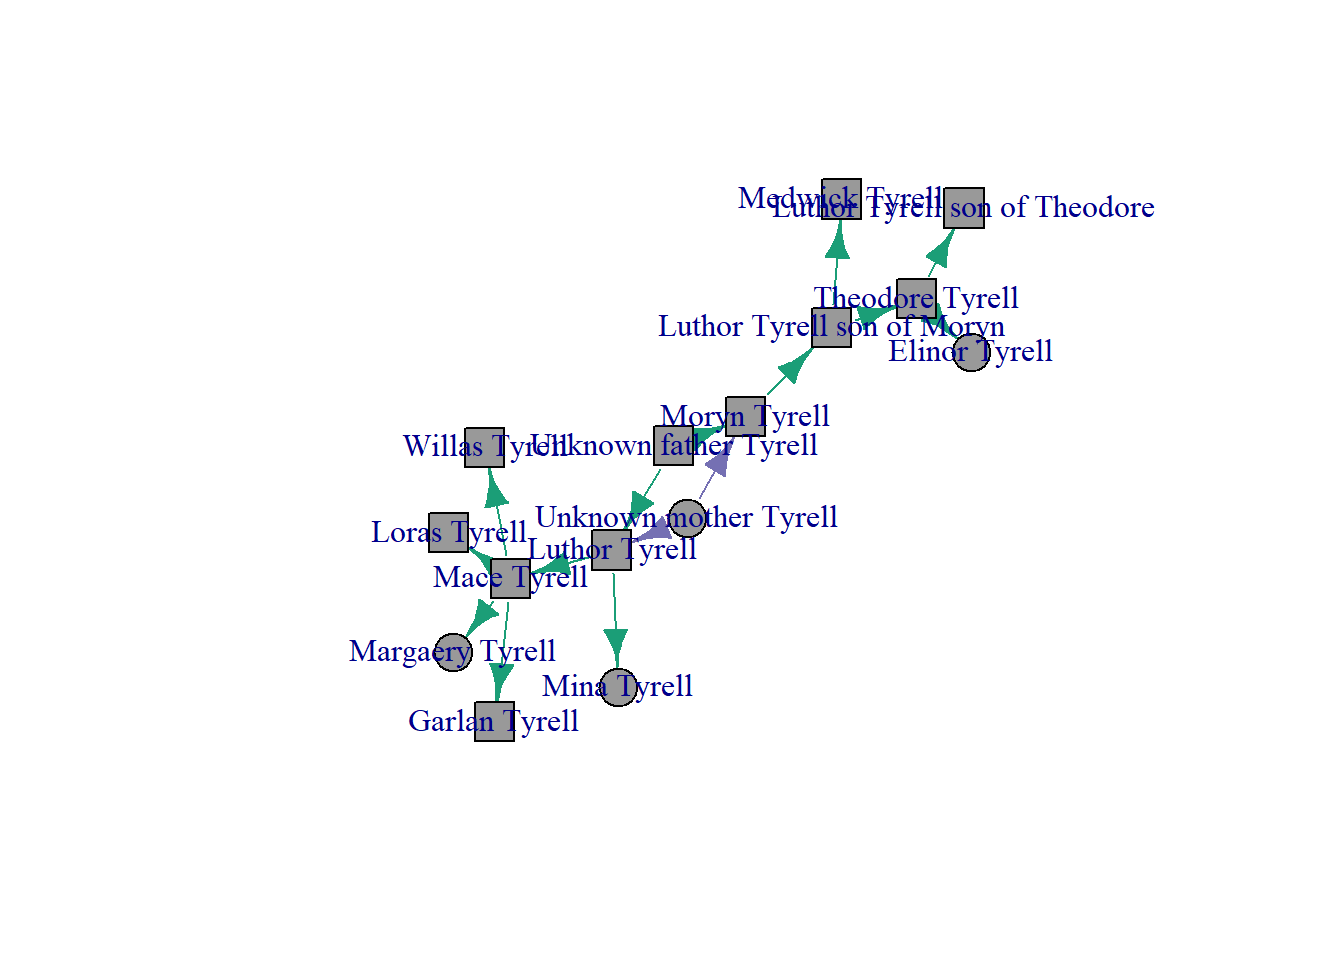
\includegraphics{book_LCC_files/figure-latex/unnamed-chunk-180-1.pdf}

Visualizar en un plot aquellos personajes que en alguno de los vértices tienen algún miembro de la casa Stark.

\begin{Shaded}
\begin{Highlighting}[]
\NormalTok{casa\_Stark\_graph }\OtherTok{=}\NormalTok{ union\_graph}
\NormalTok{casa\_Stark\_graph }\OtherTok{\textless{}{-}} \FunctionTok{delete.edges}\NormalTok{(casa\_Stark\_graph,}\FunctionTok{E}\NormalTok{(casa\_Stark\_graph)}\SpecialCharTok{$}\NormalTok{source}\SpecialCharTok{!=}\StringTok{"House Stark"} \SpecialCharTok{\&} \FunctionTok{E}\NormalTok{(casa\_Stark\_graph)}\SpecialCharTok{$}\NormalTok{target}\SpecialCharTok{!=}\StringTok{"House Stark"}\NormalTok{)}
\FunctionTok{plot}\NormalTok{(casa\_Stark\_graph)}
\end{Highlighting}
\end{Shaded}

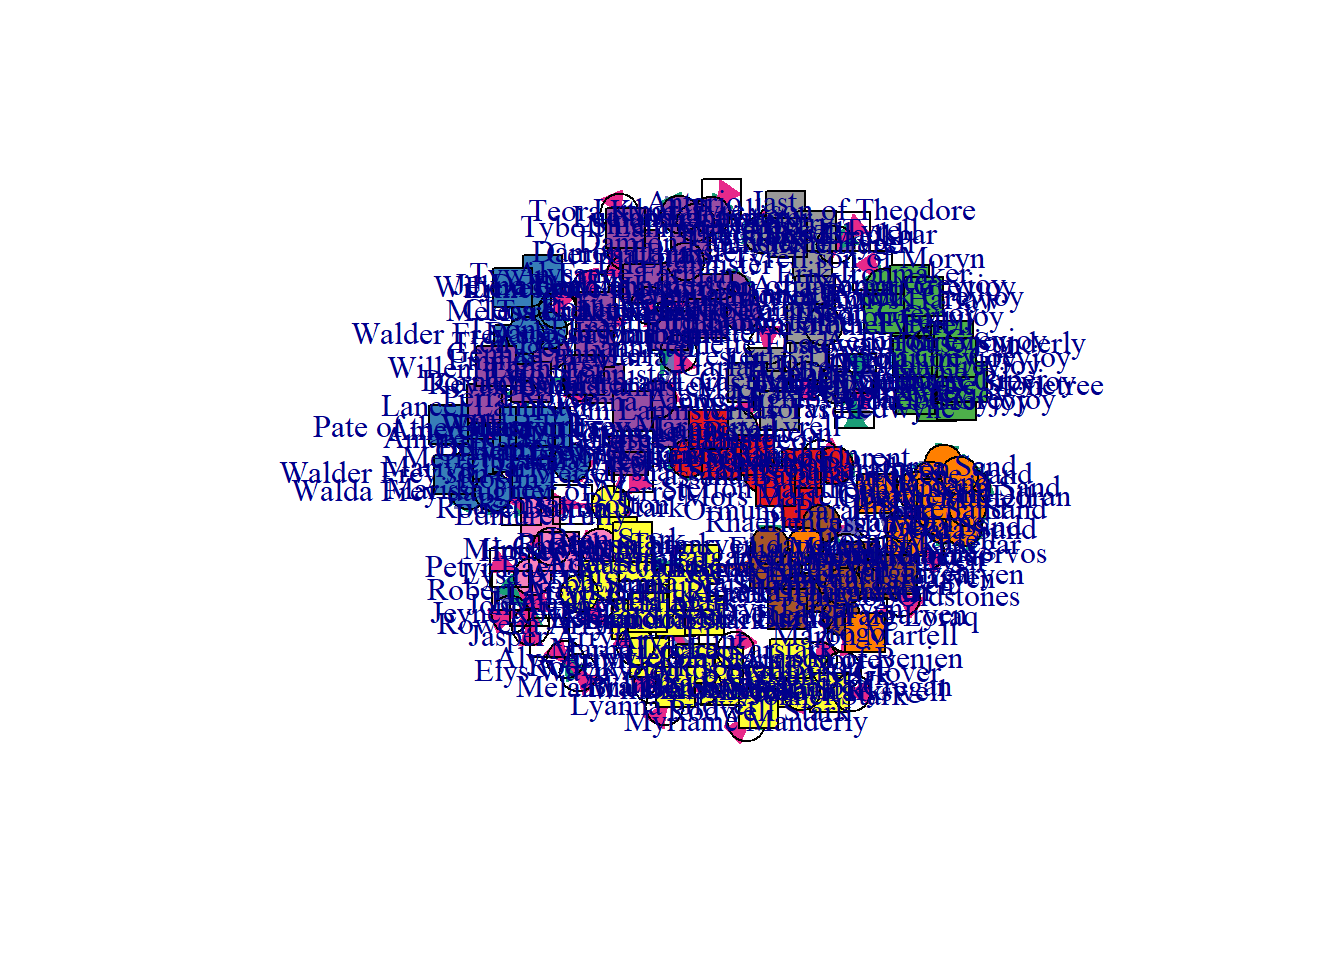
\includegraphics{book_LCC_files/figure-latex/unnamed-chunk-181-1.pdf}

Replica el análisis de Rblogger para calcular las medidas de bondad del grafo vistas en el material visto en clase. Pon algún ejemplo para cada medida.

\begin{Shaded}
\begin{Highlighting}[]
\CommentTok{\#Centrality {-}\textgreater{} Las redes con una alta \textquotesingle{}Centrality\textquotesingle{}(Importancia de los nodos en un grafo.) tienen pocos nodos con muchas conexiones; las redes con baja \textquotesingle{}Centrality\textquotesingle{} tienen muchos nodos con un numero similar de aristas.}
\CommentTok{\#Podemos calcular su \textquotesingle{}Centrality\textquotesingle{} mediante su \textquotesingle{}degree\textquotesingle{}(Número de arcos conectados a un vértice. Señala la importancia de un vértice o el nivel de actividad del vértice en la red.), \textquotesingle{}closeness\textquotesingle{}(Distancia a otros nodos. Un nodo con valor alto de este estimador es más central y puede difundir la información a muchos otros nodos.) o \textquotesingle{}eigenvector\textquotesingle{}(La medida Eigenvector Centrality se calcula como el autovalor de mayor módulo de la matriz de adyacencia que contiene los pesos.)}
\FunctionTok{centr\_degree}\NormalTok{(union\_graph, }\AttributeTok{mode =} \StringTok{"total"}\NormalTok{)}\SpecialCharTok{$}\NormalTok{centralization}
\end{Highlighting}
\end{Shaded}

\begin{verbatim}
## [1] 0.02697846
\end{verbatim}

\begin{Shaded}
\begin{Highlighting}[]
\FunctionTok{centr\_clo}\NormalTok{(union\_graph, }\AttributeTok{mode =} \StringTok{"total"}\NormalTok{)}\SpecialCharTok{$}\NormalTok{centralization}
\end{Highlighting}
\end{Shaded}

\begin{verbatim}
## Warning in centr_clo(union_graph, mode = "total"): At centrality.c:
## 2784 :closeness centrality is not well-defined for disconnected graphs
\end{verbatim}

\begin{verbatim}
## [1] 0.01414082
\end{verbatim}

\begin{Shaded}
\begin{Highlighting}[]
\FunctionTok{centr\_eigen}\NormalTok{(union\_graph, }\AttributeTok{directed =} \ConstantTok{FALSE}\NormalTok{)}\SpecialCharTok{$}\NormalTok{centralization}
\end{Highlighting}
\end{Shaded}

\begin{verbatim}
## [1] 0.9805097
\end{verbatim}

\begin{Shaded}
\begin{Highlighting}[]
\CommentTok{\#Diameter {-}\textgreater{} El camino más largo entre dos nodos}
\FunctionTok{diameter}\NormalTok{(union\_graph, }\AttributeTok{directed =} \ConstantTok{FALSE}\NormalTok{)}
\end{Highlighting}
\end{Shaded}

\begin{verbatim}
## [1] 21
\end{verbatim}

\begin{Shaded}
\begin{Highlighting}[]
\CommentTok{\#A continuación, calculamos el número de aristas entrantes y salientes de cada nodo (sumados)}

\NormalTok{union\_graph\_degree }\OtherTok{\textless{}{-}}\NormalTok{ igraph}\SpecialCharTok{::}\FunctionTok{degree}\NormalTok{(union\_graph, }\AttributeTok{mode =} \StringTok{"total"}\NormalTok{)}

\CommentTok{\#standardized by number of nodes}
\NormalTok{union\_graph\_degree\_std }\OtherTok{\textless{}{-}}\NormalTok{ union\_graph\_degree }\SpecialCharTok{/}\NormalTok{ (}\FunctionTok{vcount}\NormalTok{(union\_graph) }\SpecialCharTok{{-}} \DecValTok{1}\NormalTok{)}


\NormalTok{node\_degree }\OtherTok{\textless{}{-}} \FunctionTok{data.frame}\NormalTok{(}\AttributeTok{degree =}\NormalTok{ union\_graph\_degree,}
                          \AttributeTok{degree\_std =}\NormalTok{ union\_graph\_degree\_std) }\SpecialCharTok{\%\textgreater{}\%}
\NormalTok{  tibble}\SpecialCharTok{::}\FunctionTok{rownames\_to\_column}\NormalTok{()}

\NormalTok{union\_characters }\OtherTok{\textless{}{-}} \FunctionTok{left\_join}\NormalTok{(union\_characters, node\_degree, }\AttributeTok{by =} \FunctionTok{c}\NormalTok{(}\StringTok{"name"} \OtherTok{=} \StringTok{"rowname"}\NormalTok{))}

\NormalTok{node\_degree }\SpecialCharTok{\%\textgreater{}\%}
  \FunctionTok{arrange}\NormalTok{(}\SpecialCharTok{{-}}\NormalTok{degree) }\SpecialCharTok{\%\textgreater{}\%}
\NormalTok{  .[}\DecValTok{1}\SpecialCharTok{:}\DecValTok{10}\NormalTok{, ]}
\end{Highlighting}
\end{Shaded}

\begin{verbatim}
##            rowname degree degree_std
## 1  Quellon Greyjoy     15 0.07246377
## 2      Walder Frey     13 0.06280193
## 3   Oberyn Martell     11 0.05314010
## 4     Eddard Stark     10 0.04830918
## 5  Jason Lannister      9 0.04347826
## 6    Catelyn Stark      9 0.04347826
## 7        Jon Arryn      8 0.03864734
## 8  Margaery Tyrell      8 0.03864734
## 9       Emmon Frey      8 0.03864734
## 10 Genna Lannister      8 0.03864734
\end{verbatim}

\begin{Shaded}
\begin{Highlighting}[]
\CommentTok{\#Ahora calculamos el \textquotesingle{}Closeness\textquotesingle{} de los nodos}
\NormalTok{closeness }\OtherTok{\textless{}{-}}\NormalTok{ igraph}\SpecialCharTok{::}\FunctionTok{closeness}\NormalTok{(union\_graph, }\AttributeTok{mode =} \StringTok{"total"}\NormalTok{)}
\end{Highlighting}
\end{Shaded}

\begin{verbatim}
## Warning in igraph::closeness(union_graph, mode = "total"): At centrality.c:
## 2784 :closeness centrality is not well-defined for disconnected graphs
\end{verbatim}

\begin{Shaded}
\begin{Highlighting}[]
\CommentTok{\#standardized by number of nodes}
\NormalTok{closeness\_std }\OtherTok{\textless{}{-}}\NormalTok{ closeness }\SpecialCharTok{/}\NormalTok{ (}\FunctionTok{vcount}\NormalTok{(union\_graph) }\SpecialCharTok{{-}} \DecValTok{1}\NormalTok{)}

\NormalTok{node\_closeness }\OtherTok{\textless{}{-}} \FunctionTok{data.frame}\NormalTok{(}\AttributeTok{closeness =}\NormalTok{ closeness,}
                          \AttributeTok{closeness\_std =}\NormalTok{ closeness\_std) }\SpecialCharTok{\%\textgreater{}\%}
\NormalTok{  tibble}\SpecialCharTok{::}\FunctionTok{rownames\_to\_column}\NormalTok{()}

\NormalTok{union\_characters }\OtherTok{\textless{}{-}} \FunctionTok{left\_join}\NormalTok{(union\_characters, node\_closeness, }\AttributeTok{by =} \FunctionTok{c}\NormalTok{(}\StringTok{"name"} \OtherTok{=} \StringTok{"rowname"}\NormalTok{))}

\NormalTok{node\_closeness }\SpecialCharTok{\%\textgreater{}\%}
  \FunctionTok{arrange}\NormalTok{(}\SpecialCharTok{{-}}\NormalTok{closeness) }\SpecialCharTok{\%\textgreater{}\%}
\NormalTok{  .[}\DecValTok{1}\SpecialCharTok{:}\DecValTok{10}\NormalTok{, ]}
\end{Highlighting}
\end{Shaded}

\begin{verbatim}
##             rowname    closeness closeness_std
## 1       Sansa Stark 0.0002013288  9.726028e-07
## 2  Tyrion Lannister 0.0002012882  9.724070e-07
## 3   Tywin Lannister 0.0002011668  9.718201e-07
## 4  Joanna Lannister 0.0002005616  9.688965e-07
## 5      Eddard Stark 0.0002002804  9.675381e-07
## 6     Catelyn Stark 0.0001986492  9.596579e-07
## 7  Cersei Lannister 0.0001984915  9.588960e-07
## 8   Jaime Lannister 0.0001975894  9.545382e-07
## 9    Jeyne Marbrand 0.0001966568  9.500330e-07
## 10  Tytos Lannister 0.0001966568  9.500330e-07
\end{verbatim}

\begin{Shaded}
\begin{Highlighting}[]
\CommentTok{\#Los personajes con mayor closeness son aquellos que conectan varias historias y casas en la serie.}
\end{Highlighting}
\end{Shaded}

\begin{Shaded}
\begin{Highlighting}[]
\CommentTok{\#Betweenness {-}\textgreater{} Mide el grado en el que la información fluye a través de un vértice particular y su importancia relativa como un intermediario en la red.}

\NormalTok{betweenness }\OtherTok{\textless{}{-}}\NormalTok{ igraph}\SpecialCharTok{::}\FunctionTok{betweenness}\NormalTok{(union\_graph, }\AttributeTok{directed =} \ConstantTok{FALSE}\NormalTok{)}

\CommentTok{\# standardize by number of node pairs}
\NormalTok{betweenness\_std }\OtherTok{\textless{}{-}}\NormalTok{ betweenness }\SpecialCharTok{/}\NormalTok{ ((}\FunctionTok{vcount}\NormalTok{(union\_graph) }\SpecialCharTok{{-}} \DecValTok{1}\NormalTok{) }\SpecialCharTok{*}\NormalTok{ (}\FunctionTok{vcount}\NormalTok{(union\_graph) }\SpecialCharTok{{-}} \DecValTok{2}\NormalTok{) }\SpecialCharTok{/} \DecValTok{2}\NormalTok{)}

\NormalTok{node\_betweenness }\OtherTok{\textless{}{-}} \FunctionTok{data.frame}\NormalTok{(}\AttributeTok{betweenness =}\NormalTok{ betweenness,}
                               \AttributeTok{betweenness\_std =}\NormalTok{ betweenness\_std) }\SpecialCharTok{\%\textgreater{}\%}
\NormalTok{  tibble}\SpecialCharTok{::}\FunctionTok{rownames\_to\_column}\NormalTok{() }

\NormalTok{union\_characters }\OtherTok{\textless{}{-}} \FunctionTok{left\_join}\NormalTok{(union\_characters, node\_betweenness, }\AttributeTok{by =} \FunctionTok{c}\NormalTok{(}\StringTok{"name"} \OtherTok{=} \StringTok{"rowname"}\NormalTok{))}

\NormalTok{node\_betweenness }\SpecialCharTok{\%\textgreater{}\%}
  \FunctionTok{arrange}\NormalTok{(}\SpecialCharTok{{-}}\NormalTok{betweenness) }\SpecialCharTok{\%\textgreater{}\%}
\NormalTok{  .[}\DecValTok{1}\SpecialCharTok{:}\DecValTok{10}\NormalTok{, ]}
\end{Highlighting}
\end{Shaded}

\begin{verbatim}
##              rowname betweenness betweenness_std
## 1       Eddard Stark    6937.966       0.3254053
## 2        Sansa Stark    6197.227       0.2906630
## 3   Tyrion Lannister    5649.542       0.2649755
## 4    Tywin Lannister    5066.576       0.2376331
## 5   Joanna Lannister    4746.071       0.2226008
## 6  Rhaegar Targaryen    4295.044       0.2014466
## 7    Margaery Tyrell    4032.238       0.1891205
## 8           Jon Snow    3561.788       0.1670554
## 9        Mace Tyrell    3392.500       0.1591154
## 10   Jason Lannister    3068.500       0.1439191
\end{verbatim}

\begin{Shaded}
\begin{Highlighting}[]
\NormalTok{edge\_betweenness }\OtherTok{\textless{}{-}}\NormalTok{ igraph}\SpecialCharTok{::}\FunctionTok{edge\_betweenness}\NormalTok{(union\_graph, }\AttributeTok{directed =} \ConstantTok{FALSE}\NormalTok{)}

\FunctionTok{data.frame}\NormalTok{(}\AttributeTok{edge =} \FunctionTok{attr}\NormalTok{(}\FunctionTok{E}\NormalTok{(union\_graph), }\StringTok{"vnames"}\NormalTok{),}
           \AttributeTok{betweenness =}\NormalTok{ edge\_betweenness) }\SpecialCharTok{\%\textgreater{}\%}
\NormalTok{  tibble}\SpecialCharTok{::}\FunctionTok{rownames\_to\_column}\NormalTok{() }\SpecialCharTok{\%\textgreater{}\%}
  \FunctionTok{arrange}\NormalTok{(}\SpecialCharTok{{-}}\NormalTok{betweenness) }\SpecialCharTok{\%\textgreater{}\%}
\NormalTok{  .[}\DecValTok{1}\SpecialCharTok{:}\DecValTok{10}\NormalTok{, ]}
\end{Highlighting}
\end{Shaded}

\begin{verbatim}
##    rowname                              edge betweenness
## 1      185          Eddard Stark|Sansa Stark    4718.736
## 2      190        Rhaegar Targaryen|Jon Snow    3562.775
## 3      232       Mace Tyrell|Margaery Tyrell    3465.000
## 4      184             Eddard Stark|Jon Snow    3167.938
## 5      111  Jason Lannister|Joanna Lannister    3089.500
## 6      105 Joanna Lannister|Tyrion Lannister    3005.938
## 7      306      Sansa Stark|Tyrion Lannister    2818.271
## 8      383      Tyrion Lannister|Sansa Stark    2818.271
## 9      127  Tywin Lannister|Tyrion Lannister    2656.605
## 10     244         Luthor Tyrell|Mace Tyrell    2565.000
\end{verbatim}

Plantea en el foro de este ejercicio del CV un ejercicio a tus compañeros. Tu solución estará dentro de este ejercicio en el Book.

\begin{Shaded}
\begin{Highlighting}[]
\CommentTok{\#Visualizar en un plot aquellos personajes cuya popularidad es mayor que 0.7 y tienen definida una cultura (cultura distinta de NA)}
\NormalTok{prueba\_graph }\OtherTok{=}\NormalTok{ union\_graph}
\NormalTok{prueba\_graph }\OtherTok{\textless{}{-}} \FunctionTok{delete.vertices}\NormalTok{(prueba\_graph,}\FunctionTok{V}\NormalTok{(prueba\_graph)}\SpecialCharTok{$}\NormalTok{popularity}\SpecialCharTok{\textless{}}\FloatTok{0.7}\NormalTok{)}
\NormalTok{prueba\_graph }\OtherTok{\textless{}{-}} \FunctionTok{delete.vertices}\NormalTok{(prueba\_graph,}\FunctionTok{is.na}\NormalTok{(}\FunctionTok{V}\NormalTok{(prueba\_graph)}\SpecialCharTok{$}\NormalTok{culture))}
\FunctionTok{plot}\NormalTok{(prueba\_graph)}
\end{Highlighting}
\end{Shaded}

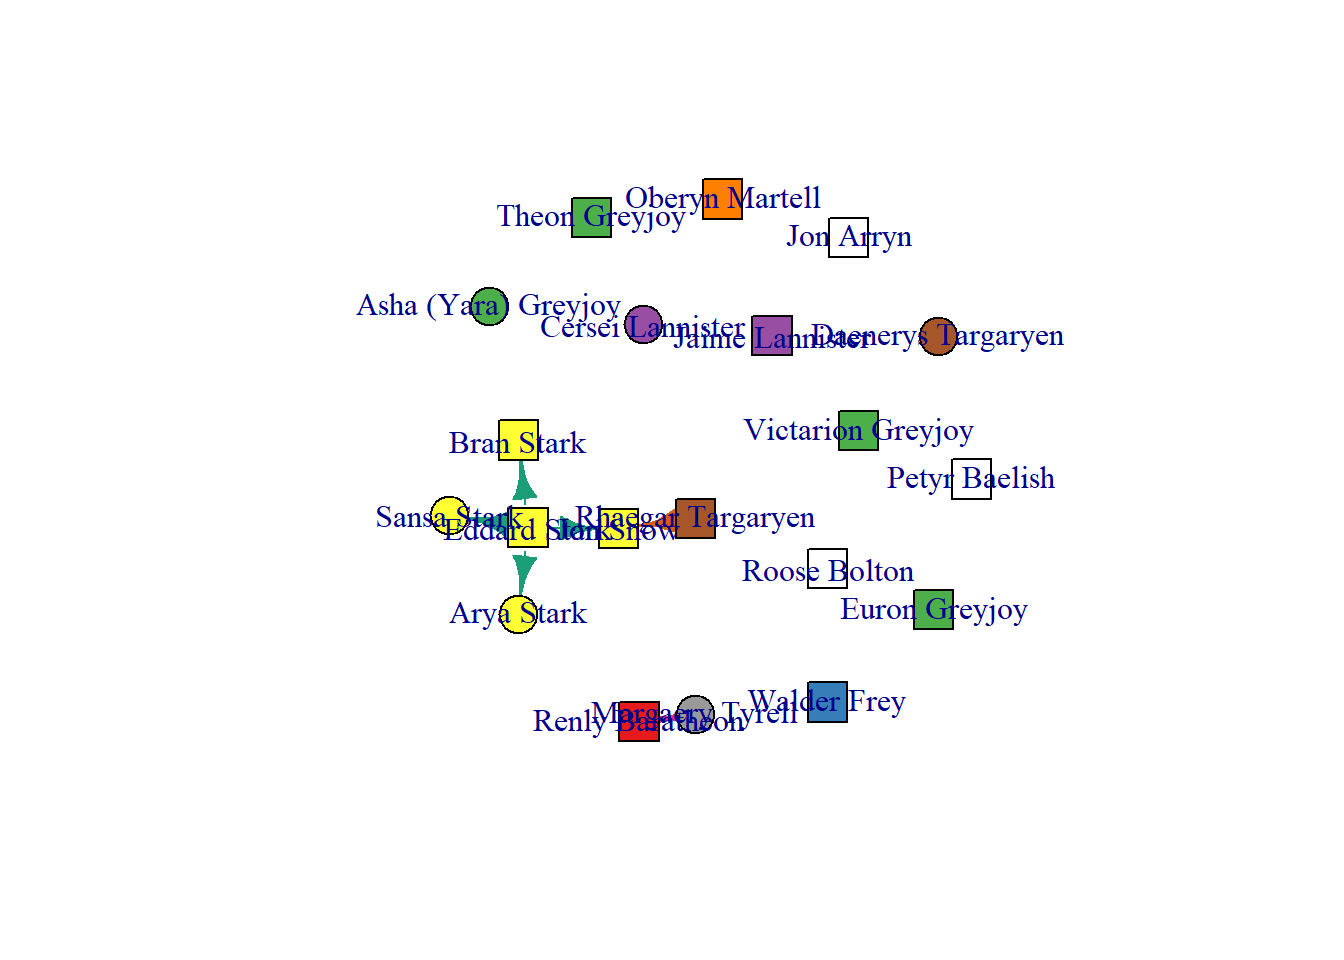
\includegraphics{book_LCC_files/figure-latex/unnamed-chunk-190-1.pdf}

Resuelve dos ejercicios planteados en el foro por tu compañeros y coloca la solución en el Book.

\begin{Shaded}
\begin{Highlighting}[]
\CommentTok{\#Muestra todos los vértices del camino entre el par de personajes más alejado sin tener en cuenta la dirección de las aristas.(Ejercicio propuesto por David Reyes Díaz)}
\FunctionTok{get\_diameter}\NormalTok{(union\_graph, }\AttributeTok{directed =} \ConstantTok{FALSE}\NormalTok{)}
\end{Highlighting}
\end{Shaded}

\begin{verbatim}
## + 22/208 vertices, named, from a9be701:
##  [1] Robyn Ryswell               Jonnel Stark               
##  [3] Cregan Stark                Brandon Stark son of Cregan
##  [5] Beron Stark                 Rodrik Stark son of Beron  
##  [7] Arya Flint                  Lyarra Stark               
##  [9] Eddard Stark                Sansa Stark                
## [11] Tyrion Lannister            Joanna Lannister           
## [13] Cersei Lannister            Joffrey Baratheon          
## [15] Margaery Tyrell             Mace Tyrell                
## [17] Luthor Tyrell               Unknown father Tyrell      
## [19] Moryn Tyrell                Luthor Tyrell son of Moryn 
## + ... omitted several vertices
\end{verbatim}

\begin{Shaded}
\begin{Highlighting}[]
\CommentTok{\#Con get\_diameter obtenemos el camino que forman los dos vertices(personajes) más alejados}

\FunctionTok{farthest\_vertices}\NormalTok{(union\_graph,}\AttributeTok{directed =} \ConstantTok{FALSE}\NormalTok{)}
\end{Highlighting}
\end{Shaded}

\begin{verbatim}
## $vertices
## + 2/208 vertices, named, from a9be701:
## [1] Robyn Ryswell Leo Blackbar 
## 
## $distance
## [1] 21
\end{verbatim}

\begin{Shaded}
\begin{Highlighting}[]
\CommentTok{\#Con farthest\_vertices obtenemos los extremos del camino calculado con get\_diameter}
\end{Highlighting}
\end{Shaded}

\begin{Shaded}
\begin{Highlighting}[]
\CommentTok{\#Numero de relaciones que hay entre la familia Lannister (Pista relaciones=arcos) (Ejercicio propuesto por Nicolás Felipe Trujillo Montero)}
\NormalTok{Lannister\_graph }\OtherTok{=}\NormalTok{ union\_graph}
\NormalTok{Lannister\_graph }\OtherTok{\textless{}{-}} \FunctionTok{delete.vertices}\NormalTok{(Lannister\_graph,}\FunctionTok{V}\NormalTok{(Lannister\_graph)}\SpecialCharTok{$}\NormalTok{house}\SpecialCharTok{!=}\StringTok{"House Lannister"}\NormalTok{)}
\FunctionTok{length}\NormalTok{(}\FunctionTok{E}\NormalTok{(Lannister\_graph))}
\end{Highlighting}
\end{Shaded}

\begin{verbatim}
## [1] 31
\end{verbatim}

  \bibliography{book.bib,packages.bib}

\end{document}
